% See "book", "report", "letter" for other types of document.

\documentclass[12pt, oneside]{article} % use larger type; default would be 10pt

\usepackage[utf8]{inputenc} % set input encoding (not needed with XeLaTeX)
\usepackage{mathptmx} % Use Times New Roman font
\usepackage{times}

%%% Examples of Article customizations
% These packages are optional, depending whether you want the features they provide.
% See the LaTeX Companion or other references for full information.

%%% PAGE DIMENSIONS %%%
\usepackage{geometry} % to change the page dimensions
\geometry{
	a4paper,
	total={21.0cm,29.7cm},
	top=2.5cm,
	bottom=2.5cm,
	right=2.5cm,
	left=3.5cm} % or letterpaper (US) or a5paper or....
% \geometry{margin=2in} % for example, change the margins to 2 inches all round
% \geometry{landscape} % set up the page for landscape
%   read geometry.pdf for detailed page layout information




%%% HEADERS & FOOTERS %%%
\usepackage{fancyhdr} % This should be set AFTER setting up the page geometry
\pagestyle{fancy} % options: empty , plain , fancy
\renewcommand{\headrulewidth}{0pt} % customize the layout...
\lhead{}\chead{}\rhead{\thepage}
\lfoot{}\cfoot{}\rfoot{}






%%% PACKAGES %%%

\usepackage{enumitem}
%\usepackage{verbatim} % adds environment for commenting out blocks of text & for better verbatim
\usepackage{pdfpages}  % to import and places other pdf file in this file
\usepackage{ragged2e} % defines new commands \centering \justify etc

\usepackage{graphicx, epstopdf} % support the \includegraphics command and options
% subfig is deliberately NOT loaded: it clashes with subcaption, and only
% subcaption's subfigure environment is used (Chapter 4 preset comparisons).
\usepackage{caption, subcaption}
% Writing Guide Ch.3: a table's title sits above the table, centered, in
% bold; a figure's title sits below the figure, in bold (figures already
% sit inside a \centering block, so their captions inherit that alignment;
% tables do not, so justification=centering is set explicitly here).
\captionsetup[table]{labelfont=bf, textfont=bf, justification=centering}
\captionsetup[figure]{labelfont=bf, textfont=bf}

\usepackage{array} % for better arrays (e.g. matrices) in maths
% Hyphenation is switched off document-wide below (\hyphenpenalty=10000),
% which suits justified body text but makes a long identifier in a narrow
% table column overflow into the margin, since it has no legal break point.
% \tabbreak restores hyphenation inside a table cell only; the \hspace{0pt}
% additionally lets the first word of a \raggedright cell hyphenate.
\newcommand{\tabbreak}{\hyphenpenalty=200\exhyphenpenalty=200\tolerance=4000\hbadness=10000\hspace{0pt}}
\usepackage{longtable} % lets a table longer than one page break across pages
                       % instead of running off the bottom; used by the data
                       % dictionary and the Chapter 5 implementation status table
\usepackage{amsmath, amssymb, amsfonts}

\usepackage{float}
\usepackage[most]{tcolorbox}
% obeyspaces: url.sty's \path (used by \tcode below) otherwise treats a
% literal space as a zero-width line-break hint rather than a printed
% character, since URLs conventionally have no real spaces in them. Plain
% inline commands like "npm run db:rebuild" do have real spaces, and
% without this option they print run together as "npmrundb:rebuild".
\usepackage[obeyspaces]{url}
\usepackage{morefloats}
\usepackage{tikz}
\usetikzlibrary{shapes, arrows, positioning}
\usepackage{pdflscape}
\usepackage{algorithm}
\usepackage{algpseudocode}
%\usepackage[nottoc,notlot,notlof]{tocbibind} % making the bibliography appears in TOC

%\usepackage[parfill]{parskip} % Activate to begin paragraphs with an empty line rather than an indent
\usepackage{indentfirst} % Activate each 1st paragraph with indent

\usepackage{setspace}
%\usepackage{times}
\usepackage{csquotes}% Recommended


\usepackage{color, colortbl}
\urlstyle{tt}
% \path{} keeps url.sty's break points after /, ., _ and - , which is what
% lets a long identifier or file path wrap inside a narrow table cell rather
% than overflowing it; the [obeyspaces] option above is what makes a literal
% space inside it print as a space rather than silently vanishing.
\newcommand{\tcode}[1]{\path{#1}}
	\definecolor{red}{rgb}{0.900, 0.200, 0.200}





%%% INDENTATION %%%

%\setlength{\parindent}{30pt} % paragraph indent size 
\setlength{\parskip}{1.3em}  % paragraph spacing
\renewcommand{\baselinestretch}{1.5}  % line spacing.. 1 for single spacing, 1.5 for one and half, 2 for double spacing





%%%% SECTION TITLE APPEARANCE %%%%

\usepackage{titlesec} % chapter heading
\usepackage{sectsty} % to renew chapter style
%\allsectionsfont{\sffamily\mdseries\upshape} % (See the fntguide.pdf for font help)
%% (This matches ConTeXt defaults)

\sectionfont{\fontsize{12}{15}\selectfont}  %% Chapter font size
\subsectionfont{\fontsize{12}{15}\selectfont}  %% Section font size
\subsubsectionfont{\fontsize{12}{15}\selectfont}  %% Subsection font size

%\titleformat{\section}{\centering}{}{1em}{}
\renewcommand{\thesection}{CHAPTER \arabic{section}:}  %% Header chapter with number
% \normalsize deliberately removed from this counter: \thesubsection is expanded
% by every \ref to a subsection as well as by the heading itself, so leaving a
% size command inside it printed cross-references at full size in the middle of
% \scriptsize table cells. Heading size is already set by \subsectionfont above.
\renewcommand{\thesubsection}{\arabic{section}.\arabic{subsection}}  %% Rename subsection with chapter number (remove perkataan Chapter)
\renewcommand{\thesubsubsection}{\arabic{section}.\arabic{subsection}.\arabic{subsubsection}}

% A local 4th-level numbered heading (e.g. 4.2.3.1 Navigation Design), used
% only inside Section 4.2.3 (User Interface Design) to match the Writing
% Guide's own worked template for that section. \secnumdepth is deliberately
% left untouched: raising it would number every \paragraph{} in the whole
% report, most of which are plain bold run-in labels never meant to carry a
% number (e.g. "ACESS Intervention:" in Chapter 2, "Domain 1" in Chapter 4).
\newcounter{uidsub}
\newcommand{\uidesignsub}[1]{%
  \stepcounter{uidsub}%
  \par\addvspace{1.3em}\noindent{\fontsize{12}{15}\selectfont\bfseries\thesubsubsection.\arabic{uidsub}\quad #1}\par\addvspace{0.3em}\nopagebreak
  \addcontentsline{toc}{subsubsection}{\protect\numberline{\thesubsubsection.\arabic{uidsub}}#1}%
}



%%% ToC (Table of Contents) APPEARANCE %%%

\usepackage[nottoc,notlof,notlot]{tocbibind} % Put the bibliography in the ToC
% The 'subfigure' option is for the obsolete subfigure/subfig packages; this
% document uses subcaption instead, and passing it here leaves \c@lotdepth
% undefined, which breaks the List of Tables on the second compilation pass.
\usepackage[titles]{tocloft} % Alter the style of the Table of Contents, List of figures and tables

\usepackage[titletoc]{appendix}
\usepackage{listings}

\renewcommand{\cftsecfont}{\rmfamily\mdseries\upshape}
\renewcommand{\cftsecpagefont}{\rmfamily\mdseries\upshape} % No bold!

\usepackage[english]{babel}
\addto\captionsenglish{
\renewcommand{\contentsname}{
\centering \normalsize TABLE OF CONTENTS   \\
\vspace{1.8cm}
\hfill PAGE \\[8mm]
}  %% To rename name of table of contents
\renewcommand{\listtablename}{
\centering \normalsize LIST OF TABLES \\
\vspace{1.8cm}
\hfill PAGE \\[8mm]
}  %% To rename list of tables
\renewcommand{\listfigurename}{
\centering \normalsize LIST OF FIGURES \\
\vspace{1.8cm}
\hfill PAGE \\[8mm]
}  %% To rename list of figures
}




%% Renaming Table and Figure Caption based on Chapter, Example, to rename from default caption, Figure 1:, to Figure 1.1:

\usepackage{chngcntr}

\counterwithin{table}{section}
\renewcommand{\thetable}{\arabic{section}.\arabic{table}}

\counterwithin{figure}{section}
\renewcommand{\thefigure}{\arabic{section}.\arabic{figure}}




\usepackage{etoolbox} %setting line spacing in TOC/LOF/T
\makeatletter
\pretocmd{\section}{\addtocontents{toc}{\protect\addvspace{-10mm}}}{}{}
\pretocmd{\subsection}{\addtocontents{toc}{\protect\addvspace{0mm}}}{}{}
\pretocmd{\subsubsection}{\addtocontents{toc}{\protect\addvspace{0mm}}}{}{}
\makeatother


%\usepackage[titles]{tocloft}
\setlength\cftbeforesecskip{2pt}  %% Set line spacing dalam ToC
\setlength\cftsecnumwidth{2.8cm}  %% Set chapter numbering width dalam ToC
\renewcommand{\cftsecleader}{\cftdotfill{\cftdotsep}}  %% Create dotted line di ToC
%\renewcommand\cftfigafterpnum{\vskip-10pt\par}
%\renewcommand\cfttabafterpnum{\vskip-10pt\par}





%%% Prevent hyphenation %%

\tolerance=1
\emergencystretch=\maxdimen
\hyphenpenalty=10000
\exhyphenpenalty=10000


\relpenalty=10000
\binoppenalty=10000




%%% BIBLIOGRAPHY / REFERENCES %%%

% apalike.bst alone only supplies author-year LABELS for the bibliography
% list; plain LaTeX's \cite still wraps them in square brackets, e.g.
% [Prensky, 2001]. The full apalike.sty package fixes that, but it also
% redefines \thebibliography from scratch using a plain-TeX-era \list call
% that conflicts with this preamble's enumitem/titlesec/tocbibind stack
% (LaTeX Error: \begin{thebibliography} ... ended by \end{thebibitemlist}).
% So only the three macros that matter are borrowed here directly, verbatim
% from apalike.sty: \cite in round parens instead of brackets (required by
% the Writing Guide's Harvard style, Chapter 3), multiple keys joined with
% "; " inside one set of parens, and no redundant [Author, Year] label
% before each reference-list entry (the year already appears in the entry
% itself, per Guide 3.6's "Author (Year). Title. Place: Publisher." format).
\makeatletter
\def\@biblabel#1{}
\def\@cite#1#2{(#1\if@tempswa , #2\fi)}
\def\@citex[#1]#2{\if@filesw\immediate\write\@auxout{\string\citation{#2}}\fi
  \def\@citea{}\@cite{\@for\@citeb:=#2\do
    {\@citea\def\@citea{; }\@ifundefined
       {b@\@citeb}{{\bf ?}\@warning
       {Citation `\@citeb' on page \thepage \space undefined}}%
{\csname b@\@citeb\endcsname}}}{#1}}
\makeatother

%\usepackage[backend=biber, style=stylename]{biblatex}
% \addbibresource{bibfile}
% \bibliographystyle{apa}

%\usepackage{natbib}
% \bibliographystyle{agsm}

%\usepackage[backend=biber, style=stylename]{\biblatex}
% \addbibresource{references}


%\usepackage[style=authoryear-ibid,backend=biber]{biblatex}
%\addbibresource{references.bib}% Syntax for version >= 1.2



%%% END Article customizations
      



%%% COVER PAGE %%%

\def \maketitleone{
\centering
\begin{titlepage}
	\bf {
	ACESS - ADAPTIVE COGNITIVE AND EDUCATIONAL \\ 
	SKILL SUPPORT
	}
	\rm
	\vskip 3in
	\bf {MUHAMMAD ALIFF BIN AFFANDI}
	\rm
	\vskip 3in
	\bf {UNIVERSITI TEKNIKAL MALAYSIA MELAKA}
	
	
\end{titlepage}

\thispagestyle{empty}

\newpage
}   


%%% END OF COVER PAGE %%%
      
         
         
%%% The "real" document content comes below...         
         
          


\begin{document}

\pagenumbering{gobble}
\newgeometry{top=5.5cm, bottom=3.5cm, right=2.5cm, left=3.5cm}
\maketitleone

\restoregeometry

\pagenumbering{roman}
\setcounter{page}{1}
\justifying


%%% FRONT MATTER %%%

\begin{center}

\vfill \null
\vspace{1cm}
{ACESS - ADAPTIVE COGNITIVE AND EDUCATIONAL SKILL SUPPORT}

\vskip 1.6in
{MUHAMMAD ALIFF BIN AFFANDI}

\vskip 1.6in
This report is submitted in partial fulfillment of the requirements for the \\
Bachelor of Computer Science (Software Development) with Honours.


\vskip 1.6in
FACULTY OF INFORMATION AND COMMUNICATION TECHNOLOGY \\
UNIVERSITI TEKNIKAL MALAYSIA MELAKA
	
\vspace{2mm}	
2026

\end{center}

\newpage

%%--------DECLARATION PAGE---------%%

\begin{center}

\vfill\null
\phantomsection
\addcontentsline{toc}{section}{DECLARATION}
\textbf{DECLARATION}

\vspace{1.5cm}
I hereby declare that this project entitled \\
ACESS - ADAPTIVE COGNITIVE AND EDUCATIONAL SKILL SUPPORT \\
is written by me and is my own effort and that no part has been plagiarized without citations.

\vspace{1.5cm}
\noindent
STUDENT \; : \underline{\hspace{8cm}} \, Date :  \underline{\hspace{2.1cm}} \\[-2mm]
(MUHAMMAD ALIFF BIN AFFANDI) \hspace{1.2cm}

\vspace{4cm}
\noindent
I hereby declare that I have read this project report and found this project report is sufficient in term of the scope and quality for the award of Bachelor of Computer Science (Software Development) with Honours.

\vspace{1.5cm}
\noindent
SUPERVISOR \; : \underline{\hspace{8cm}} \, Date :  \underline{\hspace{2.1cm}} \\[-2mm]
(TS. DR. ZURAINI BINTI OTHMAN) \hspace{0.6cm}

\end{center}

\vfill \null

\newpage

%%--------DEDICATION PAGE---------%%

\begin{center}
\phantomsection
\addcontentsline{toc}{section}{DEDICATION}
\textbf{DEDICATION}
\end{center}

\vspace{1cm}
To my beloved parents, whose endless sacrifices and unwavering faith have been my foundation through every challenge. To Ts. Dr. Zuraini Binti Othman, whose mentorship and invaluable guidance shaped not only this research but also my growth as a researcher and software developer. To all neurodivergent learners who navigate a world not yet built for them, may ACESS serve as a small step toward a future where educational platforms adapt to every mind rather than demanding that every mind adapt to them.

\vfill \null

\newpage

%%--------ACKNOWLEDGEMENT PAGE---------%%

\begin{center}
\phantomsection
\addcontentsline{toc}{section}{ACKNOWLEDGEMENT}
\textbf{ACKNOWLEDGEMENT}
\end{center}

\vspace{1cm}
I would like to express my deepest gratitude to my supervisor, Ts. Dr. Zuraini Binti Othman, for her continuous guidance, patience, and insightful feedback throughout the development of this project. Her expertise in software engineering and dedication to accessibility has been instrumental in shaping the ACESS platform into a functional and meaningful system.

My heartfelt thanks go to my family and friends, who offered unwavering emotional and moral support during the challenging moments of this journey. Their encouragement was a constant source of motivation during late nights and difficult debugging sessions.

\vfill \null

\newpage

%%--------ABSTRACT PAGE---------%%

\begin{center}
\vfill \null
\phantomsection
\addcontentsline{toc}{section}{ABSTRACT}
\textbf{ABSTRACT}
\end{center}

\vspace{1cm}

\begin{spacing}{1.1}
Traditional e-learning platforms are commonly designed using a one-size-fits-all approach, creating accessibility challenges for neurodivergent learners, particularly those with Dyslexia, Attention Deficit Hyperactivity Disorder (ADHD), and Autism Spectrum Disorder (ASD). Existing learning management systems often provide limited support for these diverse cognitive needs, resulting in increased cognitive load and reduced learning effectiveness. This project presents the design and development of the Adaptive Cognitive and Educational Skill Support (ACESS) platform, a web-based learning management system that incorporates adaptive accessibility features to support learners with different cognitive profiles. The project adopts the Agile Scrum methodology, involving iterative planning, analysis, design, and development activities across six sprints, and is implemented using Next.js, Supabase, PostgreSQL, and Tailwind CSS. Key features include configurable accessibility presets for Dyslexia, ADHD and Autism, a distraction-free reading interface, an adaptive content recommendation engine, an authoring-time accessibility compliance auditor, an AI-assisted lesson summary and question-answering assistant, embedded H5P interactive content, and educator analytics, achievements, leaderboard ranking, and certificate generation for monitoring learner progress. The platform targets WCAG 2.2 Level AA conformance, though this has not yet been independently verified through formal audit or assistive-technology testing. The developed system was evaluated through structured walkthroughs guided by task scenarios for each learner profile, complemented by an expert review conducted against WCAG 2.2 success criteria to assess usability, accessibility, and alignment with the needs of neurodivergent learners. The outcomes of this project demonstrate the feasibility of integrating accessibility and adaptive learning mechanisms into a single platform, providing a foundation for a more inclusive digital learning environment for neurodivergent learners.
\end{spacing}

\vfill \null

\newpage

\begin{center}
\vfill \null
\phantomsection
\addcontentsline{toc}{section}{ABSTRAK}
\textbf{ABSTRAK}
\end{center}

\vspace{1cm}

\begin{spacing}{1.1}
Platform e-pembelajaran tradisional sering direka menggunakan pendekatan satu-saiz-untuk-semua, yang menimbulkan cabaran kebolehcapaian bagi pelajar neurodivergen, khususnya mereka yang mengalami Disleksia, Attention Deficit Hyperactivity Disorder (ADHD), dan Autism Spectrum Disorder (ASD). Sistem pengurusan pembelajaran sedia ada sering memberikan sokongan terhad terhadap keperluan kognitif yang pelbagai ini, sekali gus meningkatkan beban kognitif dan mengurangkan keberkesanan pembelajaran. Projek ini membentangkan reka bentuk dan pembangunan platform Adaptive Cognitive and Educational Skill Support (ACESS), sebuah sistem pengurusan pembelajaran berasaskan web yang menggabungkan ciri kebolehcapaian adaptif bagi menyokong pelajar dengan profil kognitif yang berbeza. Projek ini menggunakan metodologi Agile Scrum, melibatkan aktiviti perancangan, analisis, reka bentuk dan pembangunan secara berulang merentasi enam sprint, dan dibangunkan menggunakan Next.js, Supabase, PostgreSQL, dan Tailwind CSS. Ciri utama termasuk praset kebolehcapaian boleh konfigurasi bagi Disleksia, ADHD dan Autisme, antara muka bacaan bebas gangguan, enjin pengesyoran kandungan adaptif, pengaudit pematuhan kebolehcapaian semasa penulisan kandungan, pembantu ringkasan pelajaran dan soal jawab berasaskan AI, kandungan interaktif H5P terbenam, serta analitik pendidik, pencapaian, kedudukan papan pendahulu, dan penjanaan sijil bagi memantau kemajuan pelajar. Platform ini menyasarkan pematuhan WCAG 2.2 Peringkat AA, walaupun perkara ini belum disahkan secara bebas melalui audit formal atau pengujian teknologi bantuan. Sistem yang dibangunkan ini dinilai melalui huraian berstruktur berpandukan senario tugasan bagi setiap profil pelajar, disokong oleh penilaian pakar berdasarkan kriteria kejayaan WCAG 2.2 untuk menilai kebolehgunaan, kebolehcapaian, dan keselarasan dengan keperluan pelajar neurodivergen. Hasil projek ini menunjukkan kebolehlaksanaan menggabungkan mekanisme kebolehcapaian dan pembelajaran adaptif dalam satu platform, seterusnya menyediakan asas bagi persekitaran pembelajaran digital yang lebih inklusif untuk pelajar neurodivergen.
\end{spacing}

\vfill \null

\newpage

%%% --------------------------- %%%

\vfill \null
\phantomsection
\addcontentsline{toc}{section}{TABLE OF CONTENTS}
\tableofcontents
\newpage

\vfill \null 
\phantomsection
\addcontentsline{toc}{section}{LIST OF TABLES}
{%
\let\oldnumberline\numberline%
\renewcommand{\numberline}{\tablename~\oldnumberline}%
\raggedright%
\listoftables%
}
\newpage

\vfill \null
\phantomsection
\addcontentsline{toc}{section}{LIST OF FIGURES}
{%
\let\oldnumberline\numberline%
\renewcommand{\numberline}{\figurename~\oldnumberline}%
\listoffigures%
}
\newpage

\vfill \null
\phantomsection
\addcontentsline{toc}{section}{LIST OF ABBREVIATIONS}
\begin{center}
\textbf{LIST OF ABBREVIATIONS}
\end{center}
\vspace{2cm}

\noindent
\begin{tabular}{>{\raggedright\arraybackslash\tabbreak}p{2.27cm} >{\centering\arraybackslash\tabbreak}m{0.45cm} >{\raggedright\arraybackslash\tabbreak}p{11.0cm}}
ACESS & - & Adaptive Cognitive and Educational Skill Support \\
ADHD & - & Attention Deficit Hyperactivity Disorder \\
API & - & Application Programming Interface \\
ASD & - & Autism Spectrum Disorder \\
BDA & - & British Dyslexia Association \\
COGA & - & Cognitive and Learning Disabilities Accessibility \\
CSS & - & Cascading Style Sheets \\
DDL & - & Data Definition Language \\
ERD & - & Entity Relationship Diagram \\
H5P & - & HTML5 Package (Interactive Content Format) \\
HTML & - & Hypertext Markup Language \\
JSON & - & JavaScript Object Notation \\
JWT & - & JSON Web Token \\
LMS & - & Learning Management System \\
OOAD & - & Object-Oriented Analysis and Design \\
PDF & - & Portable Document Format \\
PostgREST & - & REST API Server for PostgreSQL \\
PostgreSQL & - & Object-Relational Database Management System \\
PSM & - & Projek Sarjana Muda \\
RBAC & - & Role-Based Access Control \\
React & - & JavaScript Library for Building User Interfaces \\
RLS & - & Row-Level Security \\
RPC & - & Remote Procedure Call \\
SSR & - & Server-Side Rendering \\
Supabase & - & Open-Source Backend-as-a-Service \\
Tailwind & - & Utility-First CSS Framework \\
Tiptap & - & Headless Rich-Text Editor \\
TTS & - & Text-to-Speech \\
UDL & - & Universal Design for Learning \\
UI & - & User Interface \\
URL & - & Uniform Resource Locator \\
Vercel & - & Cloud Platform for Frontend Deployment \\
WAI & - & Web Accessibility Initiative \\
WCAG & - & Web Content Accessibility Guidelines \\
\end{tabular}

\vfill \null
\newpage

%%% MAIN MATTER %%%

\clearpage
\pagenumbering{arabic}
\setcounter{page}{1}

\setlength{\parindent}{30pt}


%==========================================================%
%==========================================================%

\newpage
\vfill \null
\thispagestyle{empty}
\begin{center}
\section{INTRODUCTION}
\end{center}
\vspace{2cm}

\subsection{Background of Study}

Teaching today is delivered through a mixture of face-to-face classes and online platforms \cite{prensky2001digital}. Digital tools have become a routine part of instruction, yet the platforms that carry the content are usually built around a single, fixed way of presenting information. This creates difficulties for neurodivergent learners, particularly those with Dyslexia, Attention Deficit Hyperactivity Disorder (ADHD) and Autism Spectrum Disorder (ASD). Whether a lesson is delivered in a classroom or online, the tools used to present it rarely offer the flexibility that different cognitive profiles require.

Most Learning Management Systems (LMS) follow a one-size-fits-all design. They present dense blocks of text, deep navigation menus and rigid assessment formats. For a neurodivergent learner these standard interfaces become barriers rather than aids. Learners with Dyslexia may struggle with the default typography and line spacing \cite{franceschini_dyslexia}, while learners with ADHD may find a cluttered dashboard and an unstructured learning path difficult to work through \cite{barkley1997adhd}.

There is therefore a need for a learning platform in which adaptation is built in rather than added on. The Adaptive Cognitive and Educational Skill Support (ACESS) platform is proposed to address this need. ACESS adjusts its interface and the way it presents content according to the accessibility preferences a learner selects. Through adjustable typography, distraction-reduced layouts and rule-based content recommendations, the platform aims to make learning material easier to work with for learners with different cognitive needs.

\subsection{Problem Statement}

Although a wide range of educational technology is available, cognitive accessibility barriers remain. The central problem addressed by this project is that current educational platforms are not designed to support learners with cognitive disabilities. The specific problems identified are as follows.

\begin{enumerate}
    \item Most e-learning platforms are not designed for learners with disabilities. Their presentation formats place a heavy load on cognitive and sensory processing, which contributes to higher dropout. Reported figures indicate that only 46\% of neurodivergent learners completed online courses compared with 74\% of their neurotypical peers \cite{spencer2022neurodiversity}, and that up to 35\% of learners with ADHD leave e-learning programmes within the first semester because of poor accessibility design \cite{burl2024neurodiversent}.
    \item Learners with disabilities lack platforms that adapt to their individual learning pace and present content in a format they can process comfortably.
    \item Employers and support organisations have no reliable way to verify the skills gained by these learners, because progress tracking and accessible certification are not provided.
    \item Educators have no single platform in which they can monitor learner progress, identify learners who need additional support, and manage accessible learning materials.
\end{enumerate}

\subsection{Objectives}

This project aims to achieve the following objectives.

\begin{enumerate}
    \item To analyse the accessibility requirements, learning challenges and content delivery needs of learners with Dyslexia, ADHD and Autism Spectrum Disorder through a literature review and a comparative study of existing e-learning platforms and accessibility standards.
    \item To develop a functional accessible web-based e-learning platform that provides rule-based adaptive content delivery, built-in text-to-speech support, adjustable accessibility settings, structured lesson and quiz management, and role-based user management for learners, educators and administrators.
    \item To implement a certificate generation module and an educator analytics dashboard that provide verifiable records of course completion and support the monitoring of individual learner progress.
    \item To evaluate the functional correctness, usability and accessibility of the developed platform through functional test cases, structured walkthroughs and expert review.
\end{enumerate}

\subsection{Scope}

The scope of the project defines the intended users of the platform and the functional modules that make up the system. ACESS is intended as a supporting tool for both classroom-based and online learning.

\subsubsection{Target Users}
\begin{itemize}
    \item \textbf{Learners.} The primary users of the learning content. The interface is designed for neurodivergent learners, although the same features remain useful to any learner.
    \item \textbf{Educators.} The authors of the courses, who require structured tools to write accessible content, manage media and monitor learner progress.
    \item \textbf{Administrators.} The operators of the platform, responsible for user and role management, course moderation and platform-level oversight.
\end{itemize}

\subsubsection{Core System Modules}
The platform is organised into the following modules.

\begin{itemize}
    \item \textbf{Authentication and Profile Module.} Manages registration, login, email verification, password reset, profile management and role-based access control for the three user roles.
    \item \textbf{Accessibility and Personalisation Module.} Stores each learner's accessibility preferences and applies them across the whole platform. It provides control over typeface, text size, spacing, background tint, distraction-free reading, motion and text-to-speech, and applies the settings without requiring the learner to reconfigure them for each course.
    \item \textbf{Course Authoring Module.} Allows educators to build courses with chapters and milestones, write lessons in a rich-text editor, embed video with time-coded questions, create interactive activities, keep a version history of each lesson, and configure quizzes, certificates and achievements.
    \item \textbf{Accessibility Compliance Module.} Checks each lesson and course against a fixed set of rules drawn from WCAG~2.2, W3C cognitive accessibility guidance and the British Dyslexia Association Style Guide, selected according to the accessibility focus declared for the course. It reports each unmet rule, names the standard the rule comes from, and offers a direct route to the fix. The result advises the educator and does not prevent publication.
    \item \textbf{Adaptive Learning Module.} Manages course enrolment, lesson progression and the rule-based recommendation engine, which suggests revision, next-lesson or advanced content according to the learner's quiz results and progress.
    \item \textbf{Assessment Module.} Delivers timed and untimed quizzes, supports multiple attempts, grades answers automatically, allows answers to be reviewed, and evaluates the result against the pass threshold set by the educator.
    \item \textbf{Analytics Module.} Records engagement measures such as time spent on a lesson, completion rate and quiz scores, and presents them to educators as per-course and per-learner views and to administrators as platform-wide views.
    \item \textbf{Certificate and Achievement Module.} Generates a personalised completion certificate in PDF form and awards badges when a learner meets the criteria defined for a course.
    \item \textbf{Interactive Content Module.} Supports five activity types (flashcards, drag-and-drop, fill-in-the-blanks, memory game and timeline), time-coded video questions, embedded H5P content, and an optional assistant that produces a plain-language lesson summary and answers questions about the lesson currently open.
    \item \textbf{Communication and Notification Module.} Manages lesson discussion threads, a contact form, and notifications raised automatically on enrolment, lesson progress, quiz attempts, new lessons and course publication.
    \item \textbf{Localisation Module.} Presents the interface in English or Bahasa Melayu, switchable by the learner and saved to the learner's profile.
\end{itemize}

\subsection{Significance of Project}

The significance of ACESS lies in moving the responsibility for accessibility from the learner to the system. Instead of expecting a learner to install browser extensions or work around an unsuitable interface, the platform applies the learner's stated preferences automatically, so that attention can be spent on the learning material itself.

For learners, the platform provides a predictable and adjustable environment that reduces reading effort and visual distraction. For educators, it provides authoring tools that make accessibility problems visible while a lesson is being written, together with analytics on learner engagement. For the faculty and for future work in this area, the project demonstrates how accessibility features can be built into the architecture of a learning platform rather than added to it afterwards.

\subsection{Expected Output}

The following outputs are expected on completion of the project.

\begin{itemize}
    \item \textbf{Adaptive web application.} A working web-based learning management system that adjusts its presentation according to the accessibility settings of the signed-in learner.
    \item \textbf{Role-based dashboards.} Three separate interfaces for learners, educators and administrators, each with its own navigation and permissions.
    \item \textbf{Accessibility settings and presets.} Three accessibility presets (Dyslexia, ADHD and Autism) together with individual controls for typeface, text size, line and word spacing, background tint, reading width, layout, motion, read-aloud and executive-function supports. A preset shows what it will change before it is applied, and every value it sets remains adjustable afterwards.
    \item \textbf{Adaptive recommendation engine.} A rule-based engine that reads quiz results and progress and produces lesson recommendations with a stated reason for each.
    \item \textbf{Course authoring tools.} A rich-text lesson editor with media upload, five interactive activity builders, in-video question authoring and version snapshots for recovery.
    \item \textbf{Accessibility compliance checker.} A checker that scores each lesson and course against a fixed rule set, reports the measured value behind each unmet rule, and points to where it can be corrected.
    \item \textbf{Quiz and assessment system.} Timed and untimed quizzes with automatic grading, attempt management and answer review.
    \item \textbf{Analytics dashboards.} Engagement and progress visualisations for educators at course and learner level, and for administrators at platform level.
    \item \textbf{Certificate and achievement system.} Automatic PDF certificate generation on course completion, with public verification, and a badge system for learner milestones.
    \item \textbf{Notification system.} Notifications raised automatically for enrolment, quiz results, new lessons and course publication.
\end{itemize}

\subsection{Conclusion}

This chapter has established the context of the ACESS project. It identified the accessibility barriers present in current educational platforms, stated the problems the project addresses, and set out the objectives, scope, significance and expected outputs of the system. The next chapter reviews the relevant literature and standards, compares four established learning management systems against the needs of neurodivergent learners, and describes the methodology, requirements and schedule adopted for the project.


%==========================================================%

\newpage
\vfill \null
\thispagestyle{empty}
\begin{center}
\section{LITERATURE REVIEW AND PROJECT METHODOLOGY}
\end{center}
\vspace{2cm}

\subsection{Introduction}

This chapter presents the academic and technical basis of the ACESS platform. It reviews current research on cognitive accessibility in digital learning, examines the frameworks that guide accessible design, and compares four widely used learning management systems against the needs of neurodivergent learners. The chapter then describes the project methodology, the software and hardware requirements, and the project schedule.

\subsection{Theoretical Frameworks for Cognitive Accessibility}

The design of ACESS rests on two established frameworks: the Universal Design for Learning (UDL) guidelines \cite{udl_guidelines} and the Web Content Accessibility Guidelines (WCAG) 2.2 \cite{wcag22}.

\subsubsection{Universal Design for Learning}
Universal Design for Learning is a framework developed by CAST \cite{udl_guidelines} for designing instruction that works for the widest possible range of learners. It rests on three principles, each of which is reflected in a corresponding feature of ACESS.

\begin{itemize}
    \item \textbf{Multiple means of engagement.} Learners differ in what motivates them, and an unstructured environment is particularly difficult for learners with ADHD \cite{barkley1997adhd}. ACESS addresses this through achievement badges and through lessons that are presented in sections rather than as a single long page.
    \item \textbf{Multiple means of representation.} Learners differ in how they take in information. A learner with Dyslexia may find spoken material easier than printed material. ACESS addresses this through built-in text-to-speech and through learner control over typeface, text size, spacing and background tint, including the Atkinson Hyperlegible typeface \cite{atkinson2021atkinson}.
    \item \textbf{Multiple means of action and expression.} Learners differ in how they demonstrate understanding. ACESS addresses this through several question formats and through quizzes that are not terminated automatically by a timer, which reduces time pressure during assessment.
\end{itemize}

\subsubsection{Web Content Accessibility Guidelines 2.2}
\label{sec:wcag}
While UDL provides the pedagogical framework, WCAG~2.2 \cite{wcag22} provides measurable technical criteria. ACESS targets Level~AA, together with four Level~AAA criteria that are particularly relevant to reading, attention and sensory differences: 1.4.8 Visual Presentation, 2.2.6 Timeouts, 2.3.3 Animation from Interactions, and 3.2.5 Change on Request. This is stated as a design target and not as a conformance claim, because no independent audit has been carried out against the platform. The accessibility statement published on the platform records this limitation, and Chapter~4 maps each targeted criterion to the ACESS feature that addresses it.

Because the barriers this project addresses are cognitive rather than purely perceptual, WCAG alone is not sufficient. ACESS therefore also draws on the W3C guidance \emph{Making Content Usable for People with Cognitive and Learning Disabilities} \cite{wcag_cognitive}, which sets out design objectives such as breaking content into manageable sections, reducing memory load and stating expectations before a task begins, and on the British Dyslexia Association Style Guide \cite{bda_style_guide}, which supplies the typographic and readability thresholds used by the platform's accessibility compliance checker. The criteria addressed most directly by ACESS are the following.

\begin{itemize}
    \item \textbf{1.4.8 Visual Presentation (AAA).} Line length is limited by a reading width expressed in characters rather than pixels, so that it stays within a comfortable range as the learner changes text size.
    \item \textbf{1.4.12 Text Spacing (AA).} Line height, word spacing and text size are set by the learner and take effect across lesson content immediately, without reloading the page.
    \item \textbf{2.2.1 Timing Adjustable (A) and 2.2.6 Timeouts (AAA).} A quiz time limit set by an educator is displayed to the learner, and the session timeout is announced by a warning thirty seconds before it takes effect.
    \item \textbf{2.3.3 Animation from Interactions (AAA).} A single motion setting reduces or removes transitions and animation across the interface.
    \item \textbf{3.2.5 Change on Request (AAA).} Applying an accessibility preset first shows the learner which settings will change and what each will change to. Text-to-speech never starts on its own.
\end{itemize}

\subsection{Neurodivergent Profiles and Interface Interventions}

Understanding the specific difficulties faced by the target learners is necessary before interface decisions can be justified. This section summarises the three profiles the platform is designed around and the response ACESS makes to each.

\subsubsection{Attention Deficit Hyperactivity Disorder}
ADHD is associated with difficulties in executive function \cite{zelazo2003executive}, affecting working memory, task initiation and sustained attention \cite{barkley1997adhd}. In a digital environment, a busy screen forces the eye to move constantly between competing elements, which accelerates fatigue \cite{munoz2003saccadic}.

The response in ACESS is a distraction-free reading mode that hides the navigation sidebar and notification area while a lesson is open, combined with a limited reading width. The width is expressed in character units rather than pixels, so it remains comfortable as the learner changes text size: 72 characters by default and 66 characters under the ADHD preset. The reading width is retained while the navigation is hidden rather than released by it. The ADHD preset also displays a persistent bar carrying the current task, an auto-save indicator and a task checklist, so that a learner who is interrupted can return to the lesson without having to work out where they were. These features are described in Chapter~4.

\subsubsection{Dyslexia}
Dyslexia involves difficulty with accurate or fluent word recognition and with spelling and decoding \cite{rello2013effect}. Research indicates that typographic adjustment can improve reading speed and comprehension \cite{franceschini_dyslexia}.

The response in ACESS is to give the learner direct control over presentation rather than relying on browser zoom. Selecting the Dyslexia preset sets the typeface to Atkinson Hyperlegible \cite{atkinson2021atkinson} (OpenDyslexic \cite{opendyslexic} is also available), raises the base text size to 19\,px, sets line spacing to 1.7, sets word spacing to 0.16\,em, which is the value required by WCAG 1.4.12, narrows the reading width to 62 characters in line with the 50 to 70 character range recommended by the British Dyslexia Association \cite{bda_style_guide}, applies a cream background to reduce glare, and enables both text-to-speech and a reading spotlight that dims the paragraphs the learner is not currently reading \cite{batanero2014accessibility}. The full set of values is given in Chapter~4.

\subsubsection{Autism Spectrum Disorder}
Learners on the autism spectrum generally work best in structured and predictable environments, and unexpected visual or auditory stimuli can cause significant distress \cite{lawson2011autism}.

ACESS responds to this from two directions. For the learner, the Autism preset keeps the reading column at the same width in every course so that pages do not change shape between lessons, removes motion, reduces colour saturation, and displays a visual schedule that lists the phases of a lesson before the learner begins, together with step-by-step guidance that always explains why a control is unavailable rather than simply disabling it. Media never plays automatically and text-to-speech never starts on its own. For the educator, the accessibility compliance checker described in Section~\ref{sec:a11y-audit} examines the draft lesson for the barriers this profile is most sensitive to: figurative language, missing learning objectives, a missing plain-language summary, and structural inconsistency with the other lessons in the same course.

\subsection{Comparative Analysis of Existing LMS Platforms}

To establish the need for ACESS, four established platforms were reviewed: Moodle \cite{moodle_software}, Canvas LMS \cite{canvas_lms}, Blackboard Learn \cite{blackboard_learn} and Google Classroom \cite{google_classroom}.

One distinction must be made before the comparison, because it determines whether the comparison is fair. A capability may be present in three different ways: \textbf{native}, meaning it is part of the product's own interface and available to every learner; \textbf{plugin}, meaning it is available only after an institution's administrator installs and configures an additional component; or \textbf{external}, meaning it is not provided by the platform and must be obtained from the operating system, the browser or separate assistive software. The comparison in Table~\ref{tab:lms_comparison} is expressed in these terms rather than as a simple yes or no, because a plugin that a learner cannot install for themselves is not equivalent to a setting the learner controls. All four platforms are mature products with established accessibility programmes; the gap identified here is specifically in learner-controlled cognitive adaptation, not in accessibility in general.

\subsubsection{Moodle}
Moodle is an open-source learning platform with wide adoption and a modular architecture \cite{moodle_architecture}. It maintains an accessibility programme and publishes its conformance work \cite{moodle_accessibility}, and its editor includes an accessibility checker that flags problems such as missing image alternative text and low contrast while an educator writes \cite{moodle_atto_a11y}. Institution-wide auditing is available through the Brickfield Accessibility Toolkit \cite{moodle_accessibility_toolkit}.

The limitation relative to this project is that the accessibility effort is directed at the correctness of authored content and at screen-reader and keyboard operability rather than at cognitive load. A learner cannot select a profile that changes typography, reading width, pacing and task scaffolding together; the nearest equivalents are administrator-selected themes and third-party blocks. Adaptive remediation depends on an educator having written conditional activity rules in advance, and no rule-based engine proposes revision content from assessment results on its own.

\subsubsection{Canvas LMS}
Canvas presents a card-based interface and publishes accessibility conformance documentation, including a Voluntary Product Accessibility Template \cite{canvas_accessibility,canvas_lms}. Its editor includes an accessibility checker that an educator can run before publishing \cite{canvas_a11y_checker}, and Microsoft Immersive Reader, which provides read-aloud, line focus and adjustable text spacing, can be integrated into Canvas pages, although it must be enabled by the institution and is invoked one page at a time rather than applied as a persistent learner setting \cite{canvas_immersive_reader}.

The limitation relative to this project is that the cognitive supports are delivered through an embedded third-party reader rather than as platform settings, so they do not persist as a learner preference across the product and do not extend to quizzes or interactive activities. Course progression remains linear unless an educator builds mastery paths manually.

\subsubsection{Blackboard Learn}
Blackboard Learn is an enterprise platform whose accessibility strategy centres on Anthology Ally, which scores uploaded course materials, gives educators remediation guidance, and generates alternative formats such as audio, ePub and tagged PDF for learners to download \cite{blackboard_ally}. Blackboard also provides a native Achievements tool for badges and certificates \cite{blackboard_achievements}.

The limitation relative to this project is that Ally operates on files rather than on the running interface. It can convert a handout into an audio file, but it does not change the typography, spacing, reading width or motion behaviour of the platform the learner is working in, and the alternative-format model moves the learner out of the course and onto a downloaded document.

\subsubsection{Google Classroom}
Google Classroom is a lightweight coordination layer over Google Workspace and inherits that ecosystem's accessibility features, including screen-reader support, keyboard navigation, and the read-aloud and dictation tools built into Google Docs and Chrome \cite{google_classroom_accessibility,google_classroom}.

The limitation relative to this project is that these supports belong to the surrounding Workspace tools rather than to Classroom. Classroom itself provides no accessibility profiles, no lesson-level engagement data and no recommendation logic; it is a system for distributing and collecting assignments rather than for supporting the learning process.

\subsection{Comparison Matrix}

Table~\ref{tab:lms_comparison} summarises the four platforms against ACESS using the native, plugin and external distinction described above. Each entry states how a capability is delivered rather than claiming that a platform is incapable of it.

{
\renewcommand{\arraystretch}{1.25}
\setstretch{1.05}
\footnotesize
\begin{longtable}{|>{\raggedright\arraybackslash\tabbreak}p{2.35cm}|>{\raggedright\arraybackslash\tabbreak}p{1.85cm}|>{\raggedright\arraybackslash\tabbreak}p{1.85cm}|>{\raggedright\arraybackslash\tabbreak}p{1.85cm}|>{\raggedright\arraybackslash\tabbreak}p{1.85cm}|>{\raggedright\arraybackslash\tabbreak}p{2.17cm}|}
\caption{LMS Accessibility Capability Comparison}
\label{tab:lms_comparison}\\
\hline
\textbf{Capability} & \textbf{Moodle} & \textbf{Canvas} & \textbf{Blackboard} & \textbf{Google Classroom} & \textbf{ACESS} \\
\hline \hline
\endfirsthead
\multicolumn{6}{l}{\footnotesize\itshape Table~\ref{tab:lms_comparison} continued from the previous page}\\
\hline
\textbf{Capability} & \textbf{Moodle} & \textbf{Canvas} & \textbf{Blackboard} & \textbf{Google Classroom} & \textbf{ACESS} \\
\hline \hline
\endhead
\hline
\multicolumn{6}{r}{\footnotesize\itshape continued on the next page}\\
\endfoot
\endlastfoot
Read-aloud of lesson text &
Plugin &
Plugin: per page \cite{canvas_immersive_reader} &
Plugin: audio alt-format \cite{blackboard_ally} &
External: Workspace \cite{google_classroom_accessibility} &
\textbf{Native}, learner setting \\ \hline
Learner-selectable dyslexia typeface and spacing &
Plugin / theme \cite{moodle_accessibility} &
Plugin: per page \cite{canvas_immersive_reader} &
External &
External &
\textbf{Native}, persistent \\ \hline
One preset changing typography, layout and pacing together &
Not provided &
Not provided &
Not provided &
Not provided &
\textbf{Native}: three presets \\ \hline
Distraction-reduced view with bounded line length &
Theme-dependent &
Not provided &
Not provided &
Minimal UI by design &
\textbf{Native}, width-bounded \\ \hline
Automatic remedial recommendation from assessment &
Educator-authored rules &
Educator-authored paths &
Educator-authored rules &
Not provided &
\textbf{Native}, rule-based \\ \hline
Authoring-time accessibility checker &
Native, editor \cite{moodle_atto_a11y} &
Native, editor \cite{canvas_a11y_checker} &
Native, file-level \cite{blackboard_ally} &
Not provided &
\textbf{Native}, profile-aware \\ \hline
Achievements and badges &
Native &
Native / add-on &
Native \cite{blackboard_achievements} &
Not provided &
\textbf{Native} \\ \hline
Lesson-level engagement data &
Native &
Native &
Native &
Limited &
\textbf{Native} \\ \hline
Reduced-motion control &
External: OS &
External: OS &
External: OS &
External: OS &
\textbf{Native} setting \\ \hline
Published WCAG position &
Documented \cite{moodle_accessibility} &
VPAT published \cite{canvas_accessibility} &
Documented \cite{blackboard_ally} &
Documented \cite{google_classroom_accessibility} &
Targeted, not audited \\ \hline
\end{longtable}
}

Three points should be made about Table~\ref{tab:lms_comparison}. First, the ACESS column is not a claim of superiority in accessibility overall. Moodle, Canvas and Blackboard all publish conformance documentation and maintain accessibility teams, whereas ACESS has not been independently audited, which is why its entry in the final row reads ``targeted, not audited''. On the available evidence those three platforms hold a stronger verified accessibility position than ACESS.

Second, ``not provided'' means the capability was not found in the vendor's current documentation for the base product. It does not mean that no third party offers it; the plugin ecosystems are large, and an institution with sufficient resources can close several of these gaps.

Third, the row that carries the argument of this project is the third one. Every platform reviewed can enlarge text, and three of the four can read text aloud. What none of them offers is a single learner-controlled preset that changes typography, reading width, content structure, pacing and task scaffolding together, without administrator involvement. That is the gap ACESS is designed to fill, and Section~\ref{sec:a11y-design} documents both what the platform does in that space and what it does not yet do.

\subsubsection{Alternative Approaches and Justification}

Several alternative technical approaches were considered before the final architecture was selected.

\begin{itemize}
    \item \textbf{Monolithic architecture against a decoupled client and server.} A single traditional server-rendered application would have been simpler to deploy. A decoupled front end \cite{nextjs_ssr} with a managed backend service \cite{supabase_docs} was chosen instead because it allows the accessibility settings to be applied on the client without reloading the page, which is necessary for the immediate feedback described in Chapter~3.
    \item \textbf{Runtime styling libraries against a utility-first framework.} Styling libraries that compute styles at runtime were considered but rejected because of their processing cost on lower-specification devices. Tailwind CSS \cite{tailwind_docs} was selected because it produces a small stylesheet and supports instant theme switching through CSS custom properties.
    \item \textbf{Document database against a relational database.} A document database would have offered a more flexible schema. A relational database was chosen because enrolments, progress records and quiz attempts depend on referential integrity, and because the recommendation engine reads across several related entities \cite{supabase_rls}.
    \item \textbf{Central state management against the framework's own context mechanism.} A dedicated state management library was considered but judged unnecessary for a single set of accessibility settings. The framework's built-in context mechanism \cite{react_docs} was used instead, which keeps the settings logic small and directly connected to the styling layer.
\end{itemize}

\subsection{Project Methodology}

The project was developed using the Agile Scrum methodology \cite{schwaber1995scrum}, an iterative framework based on short development cycles, regular review and adaptive planning. Scrum was preferred to a sequential model such as Waterfall because designing for cognitive accessibility is an empirical activity: assumptions about whether a particular interface change actually helps must be checked by using the interface, and cannot safely be deferred to the end of development.

Development was organised into six sprints of two weeks each.

\begin{itemize}
    \item \textbf{Sprint 0: requirements and setup.} Definition of the product backlog from WCAG~2.2 and UDL, creation of the project structure, and initial database schema design.
    \item \textbf{Sprints 1 and 2: core architecture.} User authentication, database schema and security policies, and role-based route protection.
    \item \textbf{Sprints 3 and 4: feature development.} The educator authoring interface (lesson editor, course creation, quiz builder) and the learner experience (enrolment, lesson viewing, progress tracking).
    \item \textbf{Sprints 5 and 6: adaptive features and refinement.} The rule-based recommendation engine, the accessibility personalisation engine, analytics dashboards, certificate generation and notifications.
\end{itemize}

Each sprint ended with a review and a retrospective. The activities carried out in each sprint are reflected in the analysis and design work reported in Chapters~3 and~4.

\subsection{Project Requirements}
\label{sec:proj-requirements}

\subsubsection{Software Requirements}

The following software was used to develop and deploy the ACESS platform.

\begin{itemize}
    \item \textbf{Visual Studio Code.} Primary code editor.
    \item \textbf{Node.js.} Runtime for the development server and the build toolchain.
    \item \textbf{Git and GitHub.} Source control, with the repository connected to the deployment platform.
    \item \textbf{Supabase CLI \cite{supabase_cli}.} Runs the complete backend stack locally, applies database changes and rebuilds the database from scratch for development and verification.
    \item \textbf{Docker Desktop \cite{docker_docs}.} Container runtime hosting the local backend stack, so that the database, authentication and storage layers can be rebuilt on the development machine without affecting the hosted project.
    \item \textbf{Vercel \cite{vercel_docs}.} Hosting platform for the deployed application, with automatic deployment from the GitHub repository.
    \item \textbf{Next.js \cite{nextjs_ssr}.} React framework providing server-side rendering, routing and request-level route protection \cite{nextjs_middleware}.
    \item \textbf{TypeScript \cite{typescript_docs}.} Used throughout the codebase for compile-time type checking.
    \item \textbf{Tailwind CSS \cite{tailwind_docs}.} Styling framework, used to apply the accessibility settings through CSS custom properties.
    \item \textbf{Supabase and PostgreSQL \cite{supabase_docs,postgresql_docs}.} Managed relational database with row-level security, token-based authentication \cite{supabase_auth}, object storage and an automatically generated data interface \cite{postgrest_docs}.
    \item \textbf{Framer Motion \cite{framer_motion_docs}.} Animation library, used for interface transitions that respect the learner's motion setting.
    \item \textbf{Tiptap \cite{tiptap_docs}.} Rich-text editor used in the educator authoring workflow.
    \item \textbf{Recharts \cite{recharts_docs}.} Charting library used for the analytics dashboards.
    \item \textbf{jsPDF \cite{jspdf_docs}.} PDF generation library used for completion certificates and administrator reports, paired with a QR-code generator that encodes each certificate's public verification address.
    \item \textbf{Google Gemini API \cite{gemini_api}.} Generative model service used for two optional and clearly labelled learner features: a plain-language lesson summary and a lesson-scoped question-answering assistant. No assessment is graded by a model.
    \item \textbf{Web Speech API \cite{webspeech_api}.} The browser's own speech synthesis interface, used for the read-aloud control. Using the browser rather than a network service keeps lesson text on the learner's device and avoids a per-request cost.
    \item \textbf{DOMPurify \cite{dompurify}.} Sanitiser applied to authored lesson content before it is displayed, which prevents harmful markup from being stored and rendered.
    \item \textbf{dnd kit \cite{dndkit}.} Drag-and-drop toolkit used by the interactive activities, and the component that makes drag-and-drop activities operable from the keyboard.
    \item \textbf{Nodemailer and Resend.} Mail services used for password recovery and notification messages.
    \item \textbf{Figma \cite{figma_software}.} Design tool used to prototype interface layouts before implementation.
\end{itemize}

\subsubsection{Hardware Requirements}

\begin{itemize}
    \item \textbf{Development workstation.} A personal computer with at least 8\,GB of memory, a multi-core processor and a solid-state drive, sufficient to run the development server and the local database stack together.
    \item \textbf{Display.} A monitor with a resolution of at least 1920 by 1080 pixels, needed to check responsive layouts and the effect of each accessibility preset.
    \item \textbf{Network connectivity.} A stable broadband connection for access to the hosted database, the deployment platform and the source repository.
    \item \textbf{Server infrastructure.} Cloud infrastructure provided by the hosting and database services, which removes the need for dedicated server hardware.
\end{itemize}

\subsubsection{Other Requirements}

\begin{itemize}
    \item \textbf{Hosted database account.} A cloud-hosted project for the production database, authentication and file storage. A separate local stack is used for schema development and verification, so that operations such as a complete database rebuild are never carried out against the hosted project.
    \item \textbf{Generative model API key.} Required only for the optional lesson summary and lesson assistant features. The platform continues to work without it.
    \item \textbf{GitHub account.} Repository hosting and the source of automated deployment.
    \item \textbf{Deployment platform account.} Linked to the repository for automated builds and hosting.
    \item \textbf{Mail service.} Used for password reset and account verification messages.
    \item \textbf{Web browser.} A current version of Chrome, Firefox or Edge for development and testing.
\end{itemize}

\subsection{Project Schedule and Milestones}

The project was carried out over six sprints of two weeks each. Table~\ref{tab:project_schedule} lists the focus and deliverables of each sprint, and Figure~\ref{fig:gantt} presents the overall schedule across fourteen weeks.

{
\renewcommand{\arraystretch}{1.3}
\setstretch{1.05}
\footnotesize
\begin{longtable}{|c|l|p{7cm}|}
\caption{Project Schedule and Milestones}
\label{tab:project_schedule}\\
\hline
\textbf{Sprint} & \textbf{Focus Area} & \textbf{Key Deliverables} \\ \hline \hline
\endfirsthead
\multicolumn{3}{l}{\footnotesize\itshape Table~\ref{tab:project_schedule} continued from the previous page}\\
\hline
\textbf{Sprint} & \textbf{Focus Area} & \textbf{Key Deliverables} \\ \hline \hline
\endhead
\hline
\multicolumn{3}{r}{\footnotesize\itshape continued on the next page}\\
\endfoot
\endlastfoot
0 & Requirements and setup & Product backlog, project structure, database schema design \\ \hline
1 & Core authentication & Registration and login, role-based route protection, email verification \\ \hline
2 & Database and security & Row-level security policies, storage configuration, data dictionary \\ \hline
3 & Educator authoring & Course creation, lesson editor, quiz builder, media upload \\ \hline
4 & Learner experience & Enrolment, lesson viewer, progress tracking, distraction-free mode \\ \hline
5 & Adaptive features and analytics & Recommendation engine, accessibility presets, analytics dashboards, certificates, notifications \\ \hline
\end{longtable}
}

\begin{figure}[H]
\centering
\footnotesize
\begin{tabular}{|>{\raggedright\arraybackslash\tabbreak}p{3.2cm}|*{14}{c|}}
\hline
\textbf{Phase} & \textbf{1} & \textbf{2} & \textbf{3} & \textbf{4} & \textbf{5} & \textbf{6} & \textbf{7} & \textbf{8} & \textbf{9} & \textbf{10} & \textbf{11} & \textbf{12} & \textbf{13} & \textbf{14} \\ \hline
\hline
Requirements Gathering & \cellcolor{blue!40} & \cellcolor{blue!40} & & & & & & & & & & & & \\ \hline
System Design & & \cellcolor{blue!40} & \cellcolor{blue!40} & \cellcolor{blue!40} & & & & & & & & & & \\ \hline
Core Architecture & & & & \cellcolor{green!40} & \cellcolor{green!40} & \cellcolor{green!40} & \cellcolor{green!40} & & & & & & & \\ \hline
Feature Development & & & & & & & \cellcolor{green!40} & \cellcolor{green!40} & \cellcolor{green!40} & \cellcolor{green!40} & & & & \\ \hline
Advanced Features & & & & & & & & & & \cellcolor{green!40} & \cellcolor{green!40} & \cellcolor{green!40} & & \\ \hline
Testing \& Refinement & & & & & & & & & & & & \cellcolor{orange!40} & \cellcolor{orange!40} & \\ \hline
Documentation \& Deployment & & & & & & & & & & & & & \cellcolor{orange!40} & \cellcolor{orange!40} \\ \hline
\end{tabular}
\caption{Gantt Chart of the ACESS Development Schedule}
\label{fig:gantt}
\end{figure}

\subsection{Summary}

This chapter has shown that existing learning management systems provide capable administrative and content-hosting features but do not address the cognitive requirements of neurodivergent learners. Where cognitive supports exist, they are typically delivered through plugins, embedded third-party readers or downloadable alternative formats rather than as settings the learner controls, and none of the four platforms reviewed offers a single preset that changes typography, layout and pacing together. The frameworks reviewed here, UDL and WCAG~2.2 supplemented by cognitive accessibility guidance and dyslexia-specific typographic recommendations, provide the basis for the design that follows. The methodology, requirements and schedule set out in this chapter define how that design was carried out. The next chapter analyses the problem in more detail and states the data, functional and non-functional requirements of the system.

%==========================================================%

\newpage
\vfill \null
\thispagestyle{empty}
\begin{center}
\section{SYSTEM ANALYSIS}
\end{center}
\vspace{2cm}

\subsection{Introduction}

This chapter translates the findings of the literature review into software engineering specifications. It begins with an analysis of the problems observed in existing educational platforms, then states the data, functional, non-functional and other requirements of the system, and finally presents the system architecture and the division of the platform into modules.

\subsection{Problem Analysis}

Chapter~2 established the general limitations of Moodle, Canvas, Blackboard Learn and Google Classroom. This section examines the operational problems that follow from those limitations and that directly shaped the design of ACESS.

\subsubsection{Current System Scenario}

Existing learning management systems present the same interface to every learner regardless of cognitive profile. A neurodivergent learner who needs a different presentation must obtain it elsewhere, through a browser extension for read-aloud, a separate tool for changing typography, or by manually closing interface elements that are in the way. The responsibility for accessibility therefore rests with the learner rather than with the system.

The flow of activity in these platforms is also linear: a learner enrols, receives content, is assessed, and completes the course. There is no feedback path by which a poor assessment result changes what the learner is offered next. If a learner performs badly on a quiz, the next topic is presented as though nothing had happened.

\begin{figure}[H]
\centering
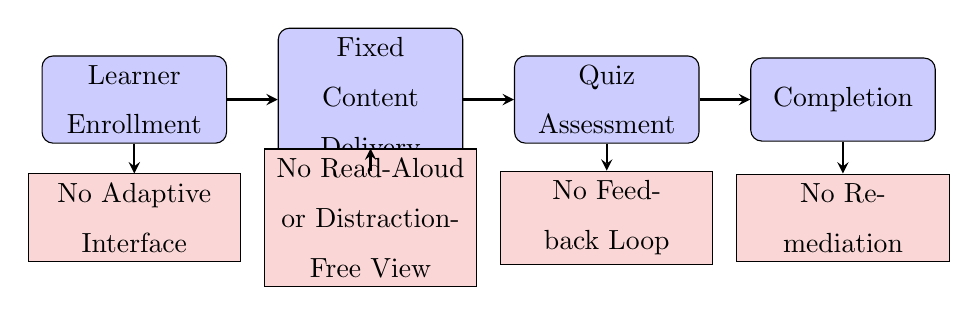
\begin{tikzpicture}[node distance=1.5cm, auto]
    \tikzstyle{block} = [rectangle, draw, fill=blue!20, text width=6em, text centered, rounded corners, minimum height=3em]
    \tikzstyle{problem} = [rectangle, draw, fill=red!20, text width=7em, text centered, minimum height=2.5em]
    \tikzstyle{arrow} = [thick,->,>=stealth]

    \node [block] (enroll) {Learner Enrollment};
    \node [block, right of=enroll, node distance=3cm] (content) {Fixed Content Delivery};
    \node [block, right of=content, node distance=3cm] (assess) {Quiz Assessment};
    \node [block, right of=assess, node distance=3cm] (complete) {Completion};

    \node [problem, below of=enroll, node distance=1.5cm] (p1) {No Adaptive Interface};
    \node [problem, below of=content, node distance=1.5cm] (p2) {No Read-Aloud or Distraction-Free View};
    \node [problem, below of=assess, node distance=1.5cm] (p3) {No Feedback Loop};
    \node [problem, below of=complete, node distance=1.5cm] (p4) {No Remediation};

    \draw [arrow] (enroll) -- (content);
    \draw [arrow] (content) -- (assess);
    \draw [arrow] (assess) -- (complete);
    \draw [arrow] (enroll) -- (p1);
    \draw [arrow] (content) -- (p2);
    \draw [arrow] (assess) -- (p3);
    \draw [arrow] (complete) -- (p4);
\end{tikzpicture}
\caption{Current System Problem Analysis Diagram}
\label{fig:problem_analysis}
\end{figure}

\subsubsection{Detailed Problem Breakdown}

Figure~\ref{fig:problem_analysis} shows this linear flow together with the point at which each barrier arises. The problems stated in Chapter~1 are analysed below in more detail.

\begin{enumerate}
    \item \textbf{Fixed typography and layout.} Standard platforms use a fixed presentation that does not respond to individual needs. Learners with Dyslexia benefit from wider letter spacing, line spacing of roughly 1.5 to 1.8, and a typeface designed to reduce confusion between similar letter shapes such as `b' and `d' \cite{atkinson2021atkinson,batanero2014accessibility}. Without these adjustments, reading is slower and fatigue accumulates, which contributes to lessons being abandoned.
    \item \textbf{Cognitive overload from navigation.} Established platforms present deeply nested menus together with dashboards showing calendars, announcements, grades and messages at the same time. For learners with ADHD \cite{barkley1997adhd} this competition for attention makes it difficult to stay with a single learning objective, and without a distraction-free mode the learner must remove the surrounding elements manually.
    \item \textbf{No adaptive remediation.} Existing assessment features record a score but do not act on it. When a learner fails a foundational topic, no revision content is recommended and no adjustment is made to the learning path. This assumes that all learners are equally ready to progress, which is particularly unsuitable for learners who need repeated exposure to a topic.
\end{enumerate}

\subsection{Requirement Analysis}

\subsubsection{Data Requirement}

ACESS requires a relational data model covering users, courses, lessons, assessments, progress and accessibility preferences. The categories of data the system must store and process are as follows.

\begin{itemize}
    \item \textbf{User data.} Account credentials, profile information such as name, avatar and role, and notification preferences. Access to user data is restricted by role.
    \item \textbf{Accessibility data.} Each learner's accessibility settings: the active preset, typeface, text size, line and word spacing, background tint, theme, layout and structure mode, motion level, read-aloud and caption settings, and the executive-function supports such as the task checklist, visual schedule, step-by-step guidance, progress timeline and auto-save indicator. These settings must persist between sessions and apply throughout the platform. They are held as a single structured document attached to the learner's profile rather than as separate columns, because the list of settings changes far more often than the rest of the schema and because every part of the system reads the settings as a whole. The trade-off this represents is discussed in Section~\ref{sec:data-dict}.
    \item \textbf{Curriculum data.} The course, chapter and lesson hierarchy, with lesson content, video references, transcripts, and metadata such as difficulty level, estimated duration and prerequisite relationships.
    \item \textbf{Assessment data.} Quiz configuration such as time limit, pass threshold and maximum attempts; questions and answer options with the correct option marked; and each learner's attempts, answers and scores.
    \item \textbf{Progress data.} Whether a lesson has been viewed and completed, the time spent on it, the state of each enrolment, and the history of quiz attempts and their outcomes.
    \item \textbf{Content and achievement data.} Interactive activity definitions, certificate records with a unique reference code, and achievement definitions with each learner's progress towards them.
    \item \textbf{Notification and communication data.} Notifications raised on enrolment, quiz attempts, new lessons and course publication, together with lesson discussion threads and contact form submissions.
\end{itemize}

The complete database schema and data dictionary are presented in Section~\ref{sec:data-dict}.

\subsubsection{Functional Requirement}

Functional requirements define what the system must do. They are grouped below by user role. Figure~\ref{fig:usecase_diagram} shows the interaction between the three actors and the functions of the system, and Tables~\ref{tab:fr_student} to~\ref{tab:fr_admin} state each requirement together with its inputs and outputs.

\begin{figure}[H]
\centering
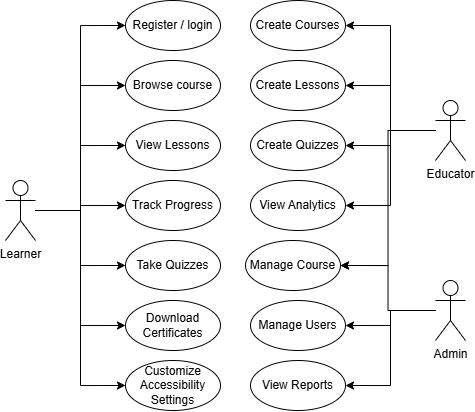
\includegraphics[width=0.8\textwidth,height=0.88\textheight,keepaspectratio]{Diagram/Figure 3.2 Use Case Diagram for ACESS Platform.png}
\caption{Use Case Diagram for the ACESS Platform}
\label{fig:usecase_diagram}
\end{figure}

\paragraph{Learner functions}

{
\renewcommand{\arraystretch}{1.2}
\setstretch{1.05}
\footnotesize
\begin{longtable}{|>{\raggedright\arraybackslash\tabbreak}p{2.09cm}|>{\raggedright\arraybackslash\tabbreak}p{2.92cm}|>{\centering\arraybackslash\tabbreak}p{1.5cm}|>{\raggedright\arraybackslash\tabbreak}p{2.09cm}|>{\raggedright\arraybackslash\tabbreak}p{3.76cm}|}
\caption{Functional Requirements of the Learner Module}
\label{tab:fr_student}\\
\hline
\textbf{Req ID} & \textbf{Description} & \textbf{Actor} & \textbf{Inputs} & \textbf{Outputs} \\ \hline \hline
\endfirsthead
\multicolumn{5}{l}{\footnotesize\itshape Table~\ref{tab:fr_student} continued from the previous page}\\
\hline
\textbf{Req ID} & \textbf{Description} & \textbf{Actor} & \textbf{Inputs} & \textbf{Outputs} \\ \hline \hline
\endhead
\hline
\multicolumn{5}{r}{\footnotesize\itshape continued on the next page}\\
\endfoot
\endlastfoot
FR-STU-01 & Registration and secure login. & Learner & Email, password & An authenticated session, and a new account and profile created automatically with the role fixed to learner. \\ \hline
FR-STU-02 & Selection of an accessibility preset or an individual setting. & Learner & Preset choice or setting value & A preview of the changes, followed by the saved settings and an immediate change to the interface without reloading the page. \\ \hline
FR-STU-03 & Course discovery and enrolment. & Learner & Course selection & A new enrolment record, and a notification to the educator who owns the course. \\ \hline
FR-STU-04 & Lesson viewing with adaptive presentation. & Learner & Navigation to a lesson & The lesson rendered at the learner's reading width, layout and typography, with navigation hidden if distraction-free mode is active. \\ \hline
FR-STU-05 & In-video questions. & Learner & Video playback reaching a stored timestamp & Playback is paused and the question is displayed over the video. \\ \hline
FR-STU-06 & Quiz attempt. & Learner & Selected answer options & The attempt is graded on the server and recorded. The correct answers are not sent to the browser before submission. \\ \hline
FR-STU-07 & Progress recording. & Learner & Time spent on the lesson page & The time spent, view count and viewed and completed status are updated. \\ \hline
FR-STU-08 & Achievement earning. & Learner & Course progress reaching a threshold & The system derives completion and records the earned achievements. A learner cannot award an achievement directly. \\ \hline
FR-STU-09 & Certificate claim and download. & Learner & Course completion & Eligibility is checked, a reference code and public verification address are issued, and the certificate is produced as a PDF. \\ \hline
FR-STU-10 & Read-aloud playback. & Learner & Selection of the Listen control & The lesson text is spoken at the learner's chosen rate. Playback never starts automatically. \\ \hline
FR-STU-11 & Adaptive recommendations. & Learner & Quiz results, viewing history, saved courses & Revision, next-lesson, near-completion and cross-course recommendations, each with the reason it was given. \\ \hline
FR-STU-12 & Saved courses and lesson discussion. & Learner & Save action, comment text & The course is added to the learner's saved list, and the comment is added to the lesson discussion thread. \\ \hline
FR-STU-13 & Lesson assistant. & Learner & A question about the lesson currently open & An answer limited to the content of that lesson, together with a stored plain-language summary of the lesson. \\ \hline
FR-STU-14 & Interface language switch. & Learner & English or Bahasa Melayu & The interface text changes immediately and the choice is saved to the learner's profile. \\ \hline
\end{longtable}
}

\paragraph{Educator functions}

Requirement FR-EDU-05 has no equivalent in the platforms surveyed in Chapter~2, and its design is described in Section~\ref{sec:a11y-audit}.

{
\renewcommand{\arraystretch}{1.2}
\setstretch{1.05}
\footnotesize
\begin{longtable}{|>{\raggedright\arraybackslash\tabbreak}p{2.09cm}|>{\raggedright\arraybackslash\tabbreak}p{2.92cm}|>{\centering\arraybackslash\tabbreak}p{1.5cm}|>{\raggedright\arraybackslash\tabbreak}p{2.09cm}|>{\raggedright\arraybackslash\tabbreak}p{3.76cm}|}
\caption{Functional Requirements of the Educator Module}
\label{tab:fr_educator}\\
\hline
\textbf{Req ID} & \textbf{Description} & \textbf{Actor} & \textbf{Inputs} & \textbf{Outputs} \\ \hline \hline
\endfirsthead
\multicolumn{5}{l}{\footnotesize\itshape Table~\ref{tab:fr_educator} continued from the previous page}\\
\hline
\textbf{Req ID} & \textbf{Description} & \textbf{Actor} & \textbf{Inputs} & \textbf{Outputs} \\ \hline \hline
\endhead
\hline
\multicolumn{5}{r}{\footnotesize\itshape continued on the next page}\\
\endfoot
\endlastfoot
FR-EDU-01 & Course creation and editing. & Educator & Title, metadata, difficulty, accessibility focus & A new or updated course, restricted to courses the educator owns. \\ \hline
FR-EDU-02 & Lesson authoring. & Educator & Rich text, headings, images, tables, links & Sanitised lesson content saved to the lesson, with a snapshot added to the version history. \\ \hline
FR-EDU-03 & Quiz and activity creation. & Educator & Question text, options, correct option, activity settings & Stored questions and options, and stored interactive activity definitions. \\ \hline
FR-EDU-04 & Asset management. & Educator & Image, document and media files & Files uploaded to course storage and recorded against the course. Instructional video is embedded from an external host rather than uploaded. \\ \hline
FR-EDU-05 & Accessibility compliance check. & Educator & The lesson draft currently open and the course accessibility focus & A score out of 100, a list of the standards met and unmet, the source of each rule, the editor tab that corrects it, and a one-click fix where one is available. The check is re-run as the lesson is written. \\ \hline
FR-EDU-06 & Learner monitoring and analytics. & Educator & Course or learner selection & Charts of progress and quiz performance, with flagging of learners at risk. \\ \hline
FR-EDU-07 & Achievement and milestone configuration. & Educator & Requirement type and threshold & Stored achievement and milestone definitions for the course. \\ \hline
FR-EDU-08 & Certificate issue and revocation. & Educator & Learner selection, revocation reason & A new or updated certificate record. A revoked certificate keeps its reference code so that verification reports the revocation rather than reporting the certificate as unknown. \\ \hline
FR-EDU-09 & Preview as a learner. & Educator & Course or lesson selection & The learner view is rendered without creating an enrolment or a progress record. \\ \hline
FR-EDU-10 & Lesson version history. & Educator & Version selection & A previous version of the lesson content is restored. \\ \hline
\end{longtable}
}

\paragraph{Administrator functions}

{
\renewcommand{\arraystretch}{1.2}
\setstretch{1.05}
\footnotesize
\begin{longtable}{|>{\raggedright\arraybackslash\tabbreak}p{2.09cm}|>{\raggedright\arraybackslash\tabbreak}p{2.92cm}|>{\centering\arraybackslash\tabbreak}p{1.5cm}|>{\raggedright\arraybackslash\tabbreak}p{2.09cm}|>{\raggedright\arraybackslash\tabbreak}p{3.76cm}|}
\caption{Functional Requirements of the Administrator Module}
\label{tab:fr_admin}\\
\hline
\textbf{Req ID} & \textbf{Description} & \textbf{Actor} & \textbf{Inputs} & \textbf{Outputs} \\ \hline \hline
\endfirsthead
\multicolumn{5}{l}{\footnotesize\itshape Table~\ref{tab:fr_admin} continued from the previous page}\\
\hline
\textbf{Req ID} & \textbf{Description} & \textbf{Actor} & \textbf{Inputs} & \textbf{Outputs} \\ \hline \hline
\endhead
\hline
\multicolumn{5}{r}{\footnotesize\itshape continued on the next page}\\
\endfoot
\endlastfoot
FR-ADM-01 & User role management. & Administrator & Target user, new role & The role is updated in both the user record and the authentication account, so that routing and database policies agree. A database guard prevents the same change being made from an ordinary session. \\ \hline
FR-ADM-02 & Course moderation. & Administrator & Approve or reject & The course status moves from pending review to published, or back to draft, and the educator is notified. \\ \hline
FR-ADM-03 & Educator application review. & Administrator & Decision and reviewer notes & The application is updated, and an approved applicant is promoted to the educator role in both the user record and the authentication account. \\ \hline
FR-ADM-04 & Official course creation. & Administrator & Course metadata & A course marked as administered by the platform, which the learner catalogue presents as an official course. \\ \hline
FR-ADM-05 & Platform analytics. & Administrator & Date range & Aggregated registrations, enrolments, completion, learning time, and figures on accessibility preset adoption and feature use. \\ \hline
FR-ADM-06 & Report generation. & Administrator & Report type and date range & A PDF report covering platform, course, learner or content coverage. \\ \hline
FR-ADM-07 & Certificate oversight. & Administrator & Search or filter & Read access to all issued certificates, including revocation status. \\ \hline
FR-ADM-08 & Enquiry handling. & Administrator & Message status change & The status of a contact form message is updated between unread, read and replied. \\ \hline
\end{longtable}
}

\subsubsection{Non-Functional Requirement}
\label{sec:nfr}

Non-functional requirements state the quality attributes the platform must satisfy.

\paragraph{Performance}
\begin{itemize}
    \item \textbf{Page response time.} Movement between pages within the application should complete within 300\,ms, so that navigation does not itself interrupt concentration.
    \item \textbf{Course loading.} Course data should be retrieved within 800\,ms on a broadband connection.
    \item \textbf{Accessibility setting response.} A change to any accessibility setting must be visible without reloading the page. This is the strictest performance requirement in the system, because a learner adjusting spacing or text size is judging the result as it changes and cannot do so if the change is delayed.
    \item \textbf{Video loading.} Instructional video is embedded from an external host rather than served by the platform, so playback start depends on that host and no target is stated for it here.
    \item \textbf{Concurrency.} The database must sustain a realistic worst-case burst of simultaneous activity for a deployment of this size without a sharp increase in response time. Chapter~6 reports load tests against this requirement.
\end{itemize}

\paragraph{Security}
\begin{itemize}
    \item \textbf{Authentication.} All sessions are secured by signed tokens held in cookies that the browser's scripts cannot read \cite{supabase_auth}, with a fifteen-minute inactivity timeout announced thirty seconds before it takes effect.
    \item \textbf{Authorisation.} Every non-public page is checked against the role held in the session before the page is rendered. This layer controls which interface a user reaches and is deliberately not treated as the security boundary; the authoritative check is repeated inside the database by row-level security policies and inside privileged server routes. Section~\ref{sec:phys-db} describes this two-layer arrangement.
    \item \textbf{Database protection.} Row-level security must be enabled on every table in the application schema, so that data isolation holds at the database itself regardless of which client issues a query. The platform currently has all 36 tables protected by 88 policies, confirmed by an executable check rather than by inspection.
    \item \textbf{Privilege guards.} Three database guards prevent a learner from forging an outcome even with a valid session: one rejects any attempt by a client to change a privileged account field, one rejects any attempt to mark a course complete outside the normal completion process, and one rejects any attempt to write a quiz score directly instead of through the grading function.
    \item \textbf{Input handling.} Authored lesson content is sanitised before it is displayed \cite{dompurify}, which is the platform's principal defence against harmful scripts stored in lesson content. All database access is parameterised, so query text is never assembled from user input. Field validation is performed in the interface and enforced again by constraints in the database.
\end{itemize}

\paragraph{Accessibility}
\begin{itemize}
    \item \textbf{WCAG target.} The platform targets WCAG~2.2 Level~AA \cite{wcag22} together with four Level~AAA criteria (1.4.8, 2.2.6, 2.3.3 and 3.2.5). Body text contrast must meet or exceed 4.5:1. This is a design target rather than an audited result, as discussed in Section~\ref{sec:a11y-design}.
    \item \textbf{Dyslexia support.} The platform must provide the Atkinson Hyperlegible \cite{atkinson2021atkinson} and OpenDyslexic \cite{opendyslexic} typefaces, line spacing adjustable between 1.0 and 3.0, and word spacing reaching at least the 0.16\,em value required by WCAG 1.4.12.
    \item \textbf{Reading width.} Lesson text must be limited by a width expressed in character units, so that line length stays within a comfortable range as text size changes: 72 characters by default, 62 under the Dyslexia preset and 66 under the ADHD preset. The limit must be retained when navigation is hidden.
    \item \textbf{ADHD and Autism support.} A single motion setting must reduce or remove animation across the interface. No media may play automatically, and read-aloud must never begin without an explicit action by the learner.
    \item \textbf{Screen reader compatibility.} Interface components must expose the correct accessible names and states, navigation must be built from real links rather than click handlers, and every interactive activity must be operable from the keyboard. It should be noted that no assistive technology testing has been carried out against this build, so this requirement is currently satisfied by construction and code review only.
\end{itemize}

\paragraph{Usability}
\begin{itemize}
    \item \textbf{Consistent navigation.} The navigation structure must remain the same across all pages of a role, so that the interface stays predictable.
    \item \textbf{Error prevention.} Destructive actions, such as an educator deleting a course, must require an explicit confirmation step.
\end{itemize}

\paragraph{Reliability}
\begin{itemize}
    \item \textbf{Data integrity.} The schema must enforce referential integrity so that records cannot be left orphaned, for example a progress record without a valid enrolment.
    \item \textbf{Backup and reproducibility.} The hosted database relies on the provider's managed backup. Independently of that, the whole schema must be reconstructible from version-controlled definitions and the demonstration dataset from a repeatable script, so that a complete working database can be rebuilt from the project repository alone.
\end{itemize}

\paragraph{Maintainability and scalability}
\begin{itemize}
    \item \textbf{Modular architecture.} The codebase must separate data retrieval from interactive presentation, so that each part can be changed independently.
    \item \textbf{Normalisation.} The schema must follow Third Normal Form, other than the deliberate exceptions documented in Section~\ref{sec:data-dict}, so that data is not duplicated as the number of courses and learners grows.
\end{itemize}

\subsubsection{Other Requirements}

The software and hardware listed in Section~\ref{sec:proj-requirements} were selected for the following reasons.

\begin{itemize}
    \item \textbf{Next.js and React \cite{nextjs_ssr}.} Rendering pages on the server reduces the amount of code the browser must process before a page becomes usable, which supports the page-load requirement above. The framework also provides a single place to check a user's role before a protected page is rendered \cite{nextjs_middleware}.
    \item \textbf{Supabase and PostgreSQL \cite{supabase_docs}.} Row-level security \cite{supabase_rls} enforces data isolation inside the database rather than only in application code, so progress and assessment data remain separated per learner regardless of how a query reaches the database.
    \item \textbf{Tailwind CSS \cite{tailwind_docs}.} The framework applies the accessibility settings through CSS custom properties, which allows typography and colour to change immediately without re-rendering the page.
    \item \textbf{TypeScript \cite{typescript_docs}.} Type checking across the codebase reduces the risk of errors in critical paths such as quiz scoring and the application of accessibility settings.
    \item \textbf{Vercel \cite{vercel_docs}.} Deployment close to the user keeps page transitions fast, which supports the performance requirements stated above.
\end{itemize}

\subsection{System Architecture}

ACESS uses a decoupled client and server architecture in which the browser communicates with a managed database service through a generated data interface, with a small number of server routes reserved for privileged operations.

\subsubsection{Context Diagram}
The context diagram gives the highest-level view of the system, showing its boundary and the external parties and services it interacts with.

\begin{figure}[H]
\centering
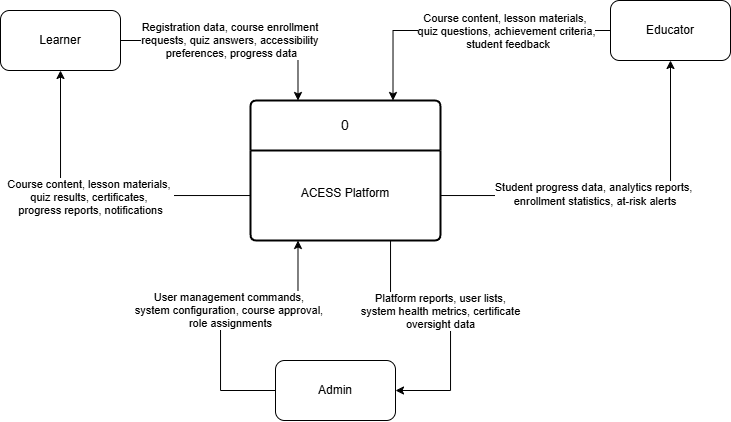
\includegraphics[width=0.8\textwidth,height=0.88\textheight,keepaspectratio]{Diagram/Figure 3.3 Context Diagram.png}
\caption{Context Diagram}
\label{fig:context_diagram}
\end{figure}

As shown in Figure~\ref{fig:context_diagram}, ACESS is the central processing system. The three human actors are the learner, who consumes content and generates progress data; the educator, who authors content and configures assessments; and the administrator, who oversees the platform. Four external services sit on the system boundary: a mail provider for password recovery and notification messages; an external video host from which instructional video is embedded rather than uploaded; a generative model service used only for the optional lesson summary and lesson assistant; and the browser's own speech synthesis engine \cite{webspeech_api}, which performs read-aloud on the learner's own device. The last of these is a deliberate choice: it avoids a per-request cost and means that lesson text does not have to leave the device in order to be read aloud.

\subsubsection{System Architecture Diagram}

\begin{figure}[H]
\centering
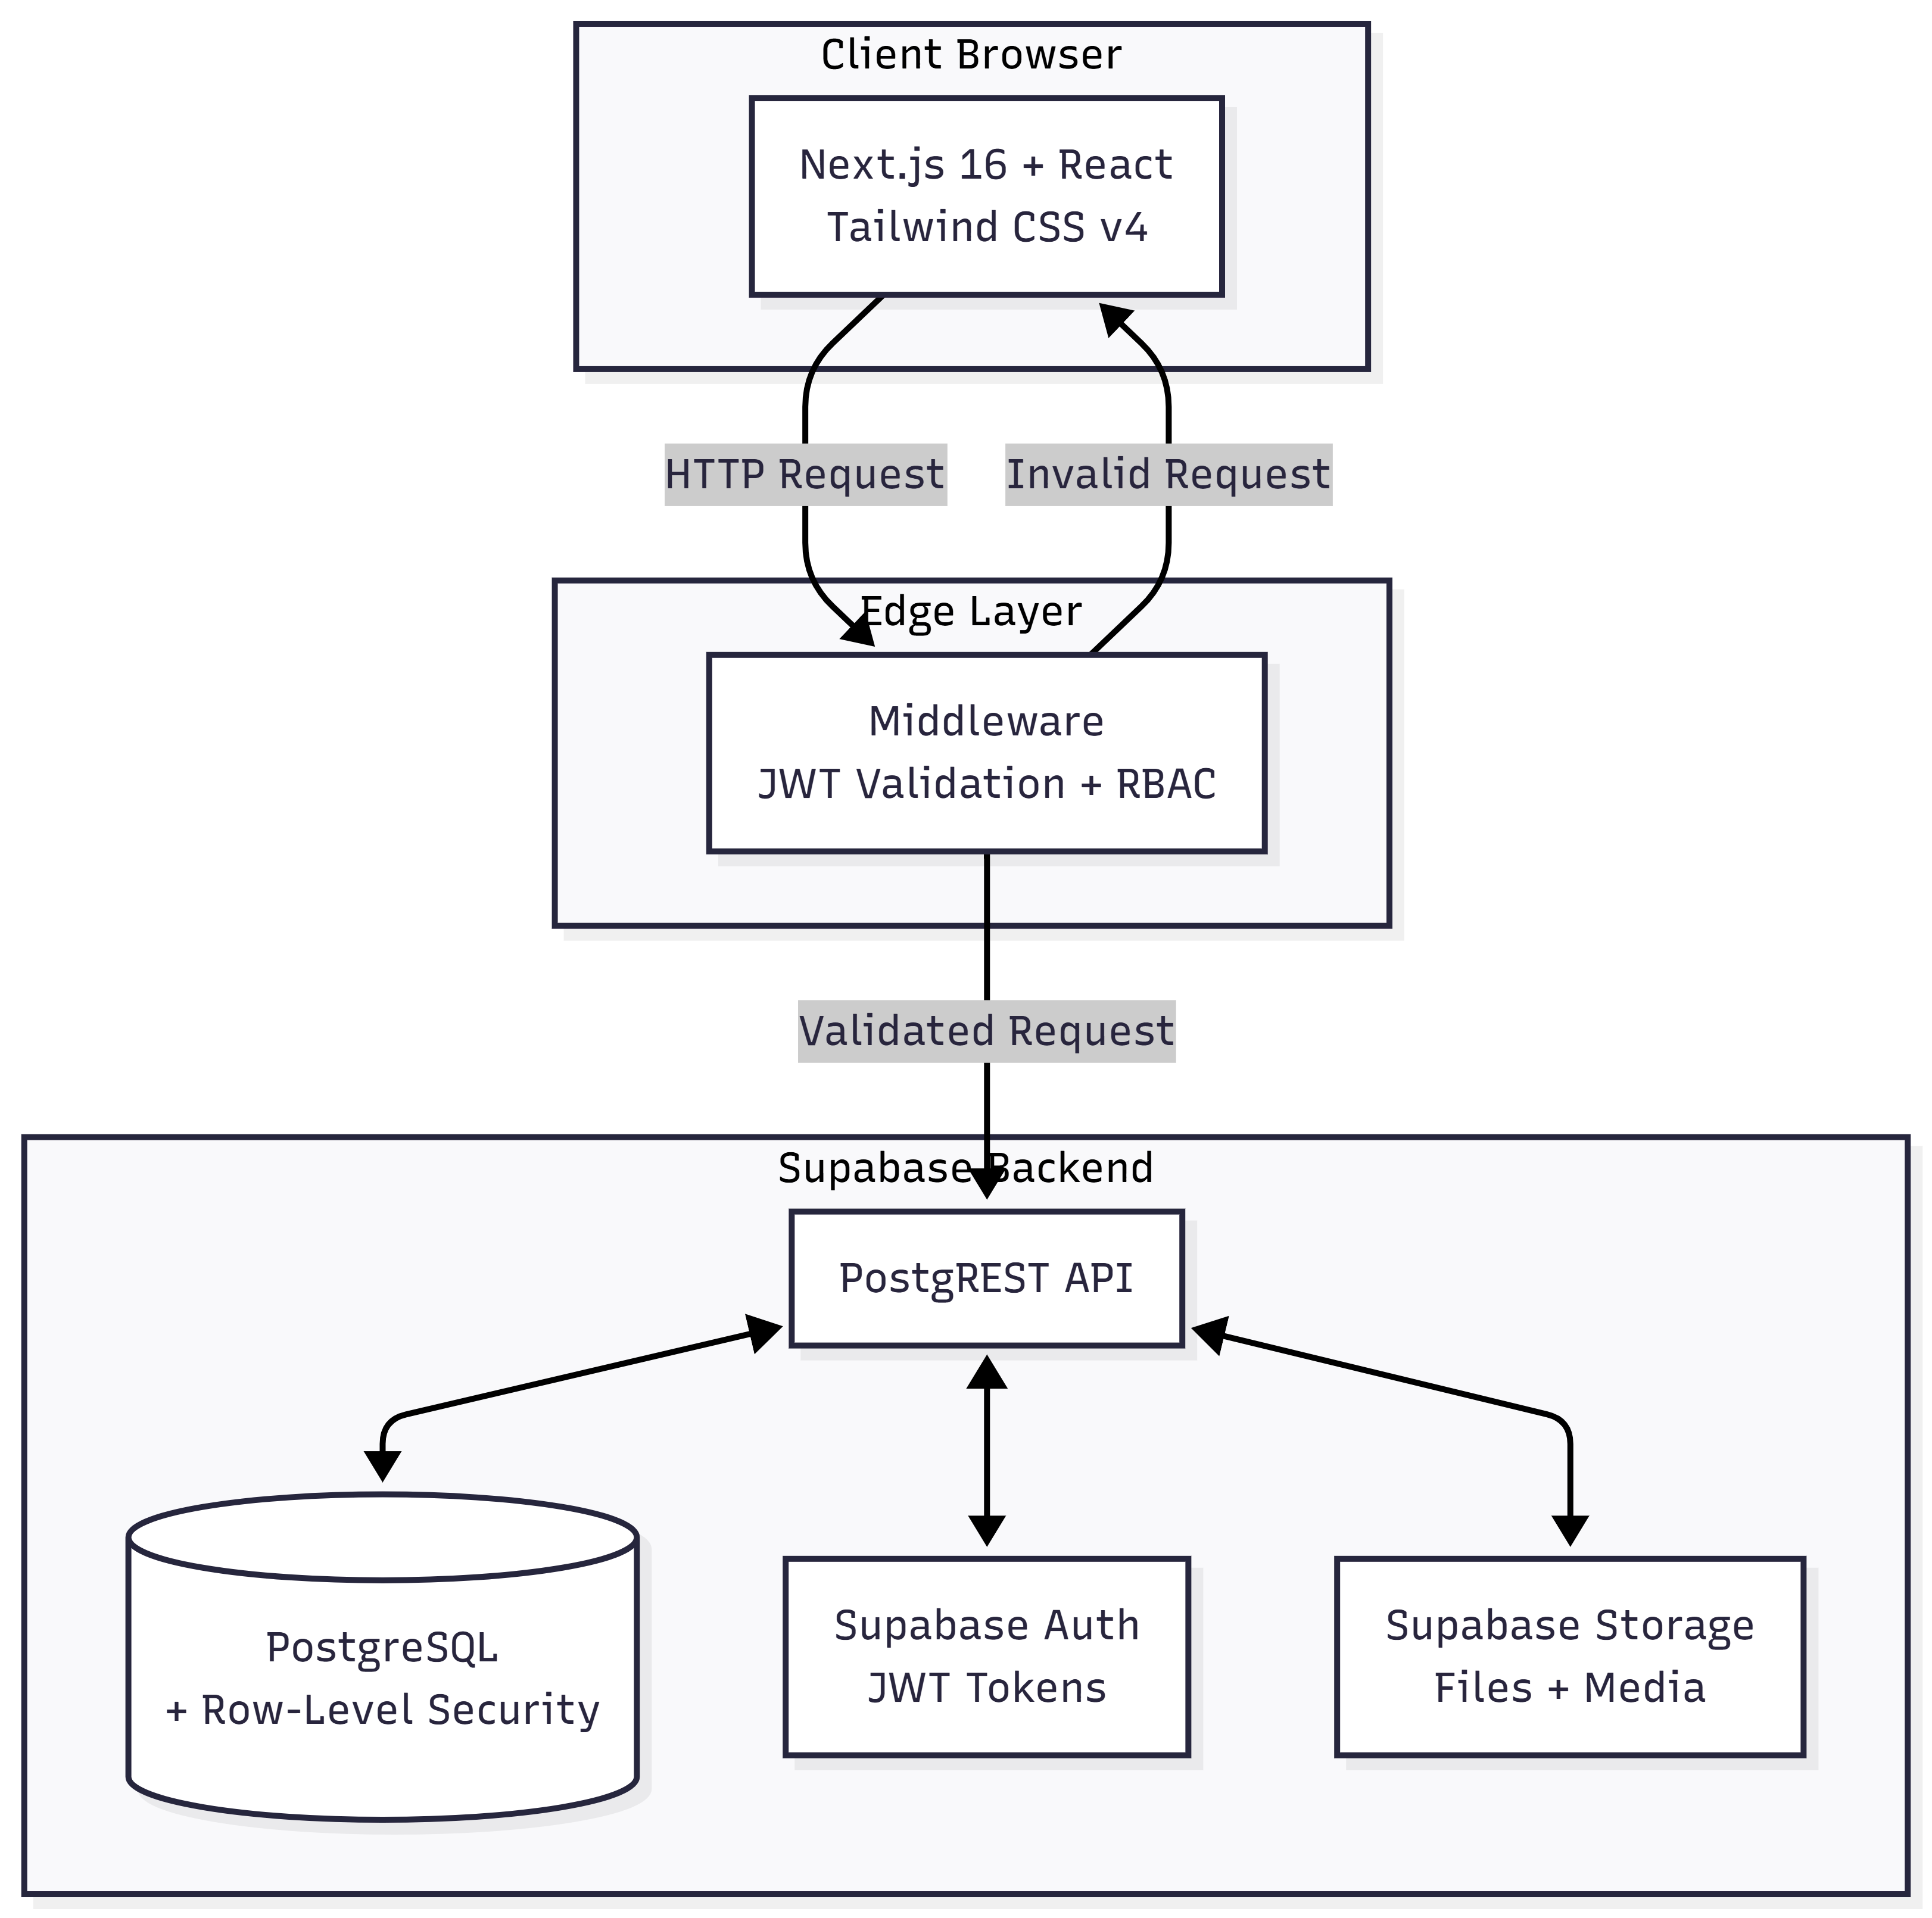
\includegraphics[width=0.8\textwidth,height=0.88\textheight,keepaspectratio]{Diagram/Figure 3.4 System Architecture Diagram.png}
\caption{System Architecture Diagram}
\label{fig:system_architecture}
\end{figure}

Figure~\ref{fig:system_architecture} shows the three tiers of the architecture.

\begin{itemize}
    \item \textbf{Presentation tier.} The interface is built with the Next.js App Router. Data retrieval is performed on the server so that less code has to be sent to the browser, and interactive behaviour such as the lesson editor and the quiz interface runs on the client. Styling is applied through CSS custom properties, which is what allows the accessibility settings to take effect immediately.
    \item \textbf{Route protection layer.} A request check runs before every non-public page. It validates the session, refuses suspended or deleted accounts, and admits the learner, educator or administrator area according to the role held in the session. It reads the role from the session rather than from the database in order to avoid a database query on every request. The authoritative role check is repeated in the database and in privileged server routes, so this layer decides which interface a user sees rather than which data they may reach.
    \item \textbf{Data tier.} A managed PostgreSQL database is exposed over a generated data interface \cite{postgrest_docs}. Security is written into the schema itself: 88 row-level security policies across all 36 tables, three guards that prevent privilege and outcome forgery, and two operations that must not be decided by the client, quiz grading and course completion, implemented as trusted database functions rather than as browser logic.
    \item \textbf{Storage tier.} Three storage areas hold uploaded files: course assets such as lesson media and thumbnails, educator-supplied certificate designs, and profile pictures. All three are readable by address because the application renders those addresses directly in the page, while write access is restricted by policy, and a learner may write only within a folder belonging to their own account. Instructional video is not stored here, and completion certificates are produced in the browser at the moment of download rather than stored as files.
\end{itemize}

\subsubsection{Deployment Diagram}

\begin{figure}[H]
\centering
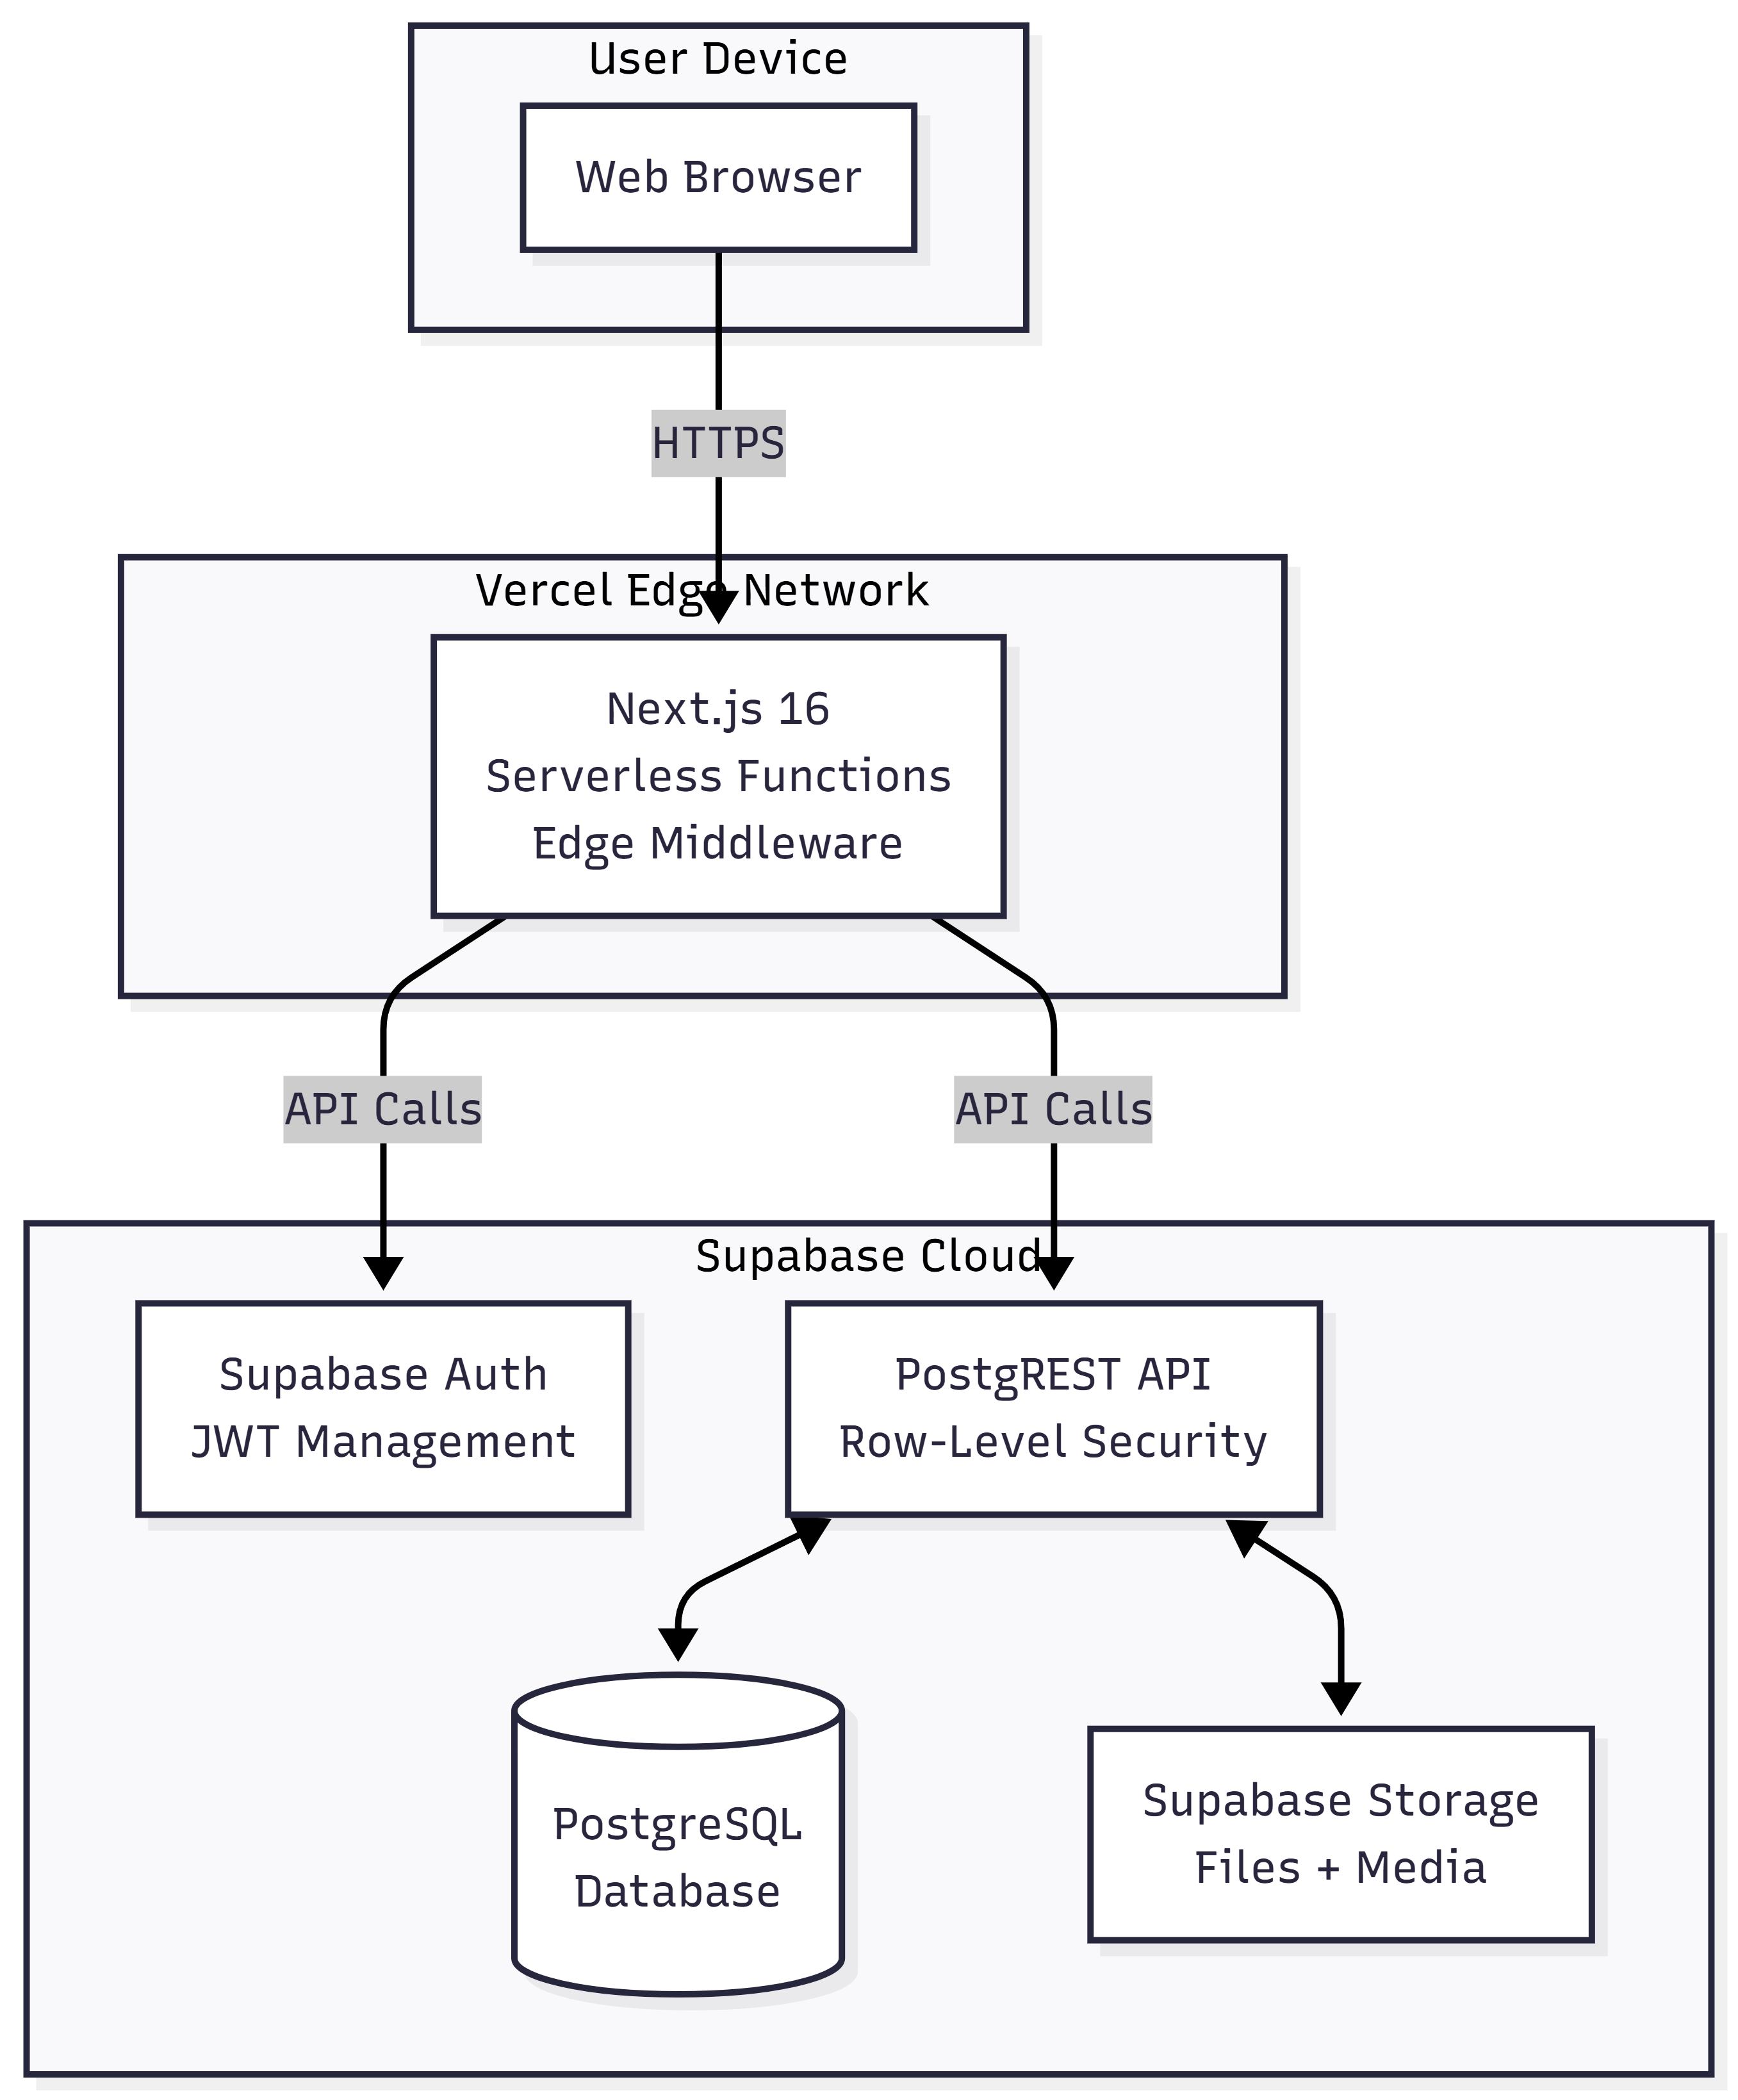
\includegraphics[width=0.8\textwidth,height=0.88\textheight,keepaspectratio]{Diagram/Figure 3.5 Deployment Diagram.png}
\caption{Deployment Diagram}
\label{fig:deployment_diagram}
\end{figure}

Figure~\ref{fig:deployment_diagram} shows how the components are distributed. The application is deployed to a serverless hosting platform \cite{vercel_docs}, which rebuilds it from the source repository on each release. The backend runs on managed cloud infrastructure and exposes the schema through a generated data interface \cite{postgrest_docs} used both by the browser, under row-level security, and by the server routes. Four operations, namely account provisioning, role changes, recommendation generation and certificate issue, require privileges the learner does not have and are therefore implemented as server routes rather than as calls from the browser.

A second, complete copy of the same backend runs locally in containers for development, comprising the database, the authentication service, the data interface, storage and the administration console. Because the schema is defined entirely by version-controlled definitions, this local environment can be rebuilt from empty on demand, which is what makes the database evidence presented in Section~\ref{sec:phys-db} reproducible rather than a description of a single mutable instance.

\subsection{Module Design}

The system is divided into the following modules.

\begin{itemize}
    \item \textbf{Learner module.} Course discovery, enrolment, lesson viewing, quiz attempts and progress.
    \item \textbf{Educator module.} Course and lesson authoring, the lesson editor, quiz and activity creation, and media upload.
    \item \textbf{Administrator module.} User and role management, course moderation, educator application review, platform analytics and reporting.
    \item \textbf{Accessibility module.} Loads the learner's stored settings, resolves any conflicts between them, and applies the result to the whole interface, from which typography, colour, reading width and motion behaviour are derived.
    \item \textbf{Accessibility compliance module.} A checking engine shared by two views: the lesson editor, which re-runs it on the draft as it is written, and the course-level report, which runs the same rules against saved lessons. Because the engine has no side effects and produces the same result for the same input, the two views always agree.
    \item \textbf{Interactive activity module.} Five activity types together with in-video questions and embedded H5P content. Quiz assessment is handled separately and is graded in the database rather than in this module.
    \item \textbf{Analytics module.} Aggregates lesson progress, quiz attempts and accessibility usage into charts, giving educators a course-level view and administrators a platform-level view, including which accessibility features are actually being used.
\end{itemize}

\subsection{Summary}

This chapter has analysed the specifications required to build the ACESS platform. It examined the problems in existing educational systems in detail, stated the data, functional, non-functional and other requirements, presented the system architecture through context, architecture and deployment diagrams, and described the division of the platform into modules. The next chapter translates these requirements into a system design, covering the behaviour of each role, the user interface, the database model, the accessibility design and the physical implementation of the database.

%==========================================================%

\newpage
\vfill \null
\thispagestyle{empty}
\begin{center}
\section{SYSTEM DESIGN}
\end{center}
\vspace{2cm}

\subsection{Introduction}

This chapter translates the requirements established in Chapter~3 into a system design. It follows the order set out in the writing guide. The high-level design is presented first, covering the behaviour of each role, the interactions between the system components, the user interface, and the conceptual and logical database model. The accessibility design, which is the substantive contribution of this project, follows. The data dictionary is then presented, and the chapter closes with the detailed design of the software components and the physical database.

Two features of this chapter should be noted. First, the figures are evidence rather than illustration: the interface figures are screenshots of the running system taken against a database that can be rebuilt from the project repository, and the entity relationship diagrams are generated from that database's own catalogue rather than drawn by hand. Second, Section~\ref{sec:a11y-design} states both what the accessibility implementation does and what it does not do, because an accessibility design that reports only its successes would be of limited value to a reader trying to judge it.

\subsection{High-Level Design}

\subsubsection{Behavioural Design}

Activity diagrams model the workflow of each role.

\paragraph{Learner workflow}

\begin{figure}[H]
\centering
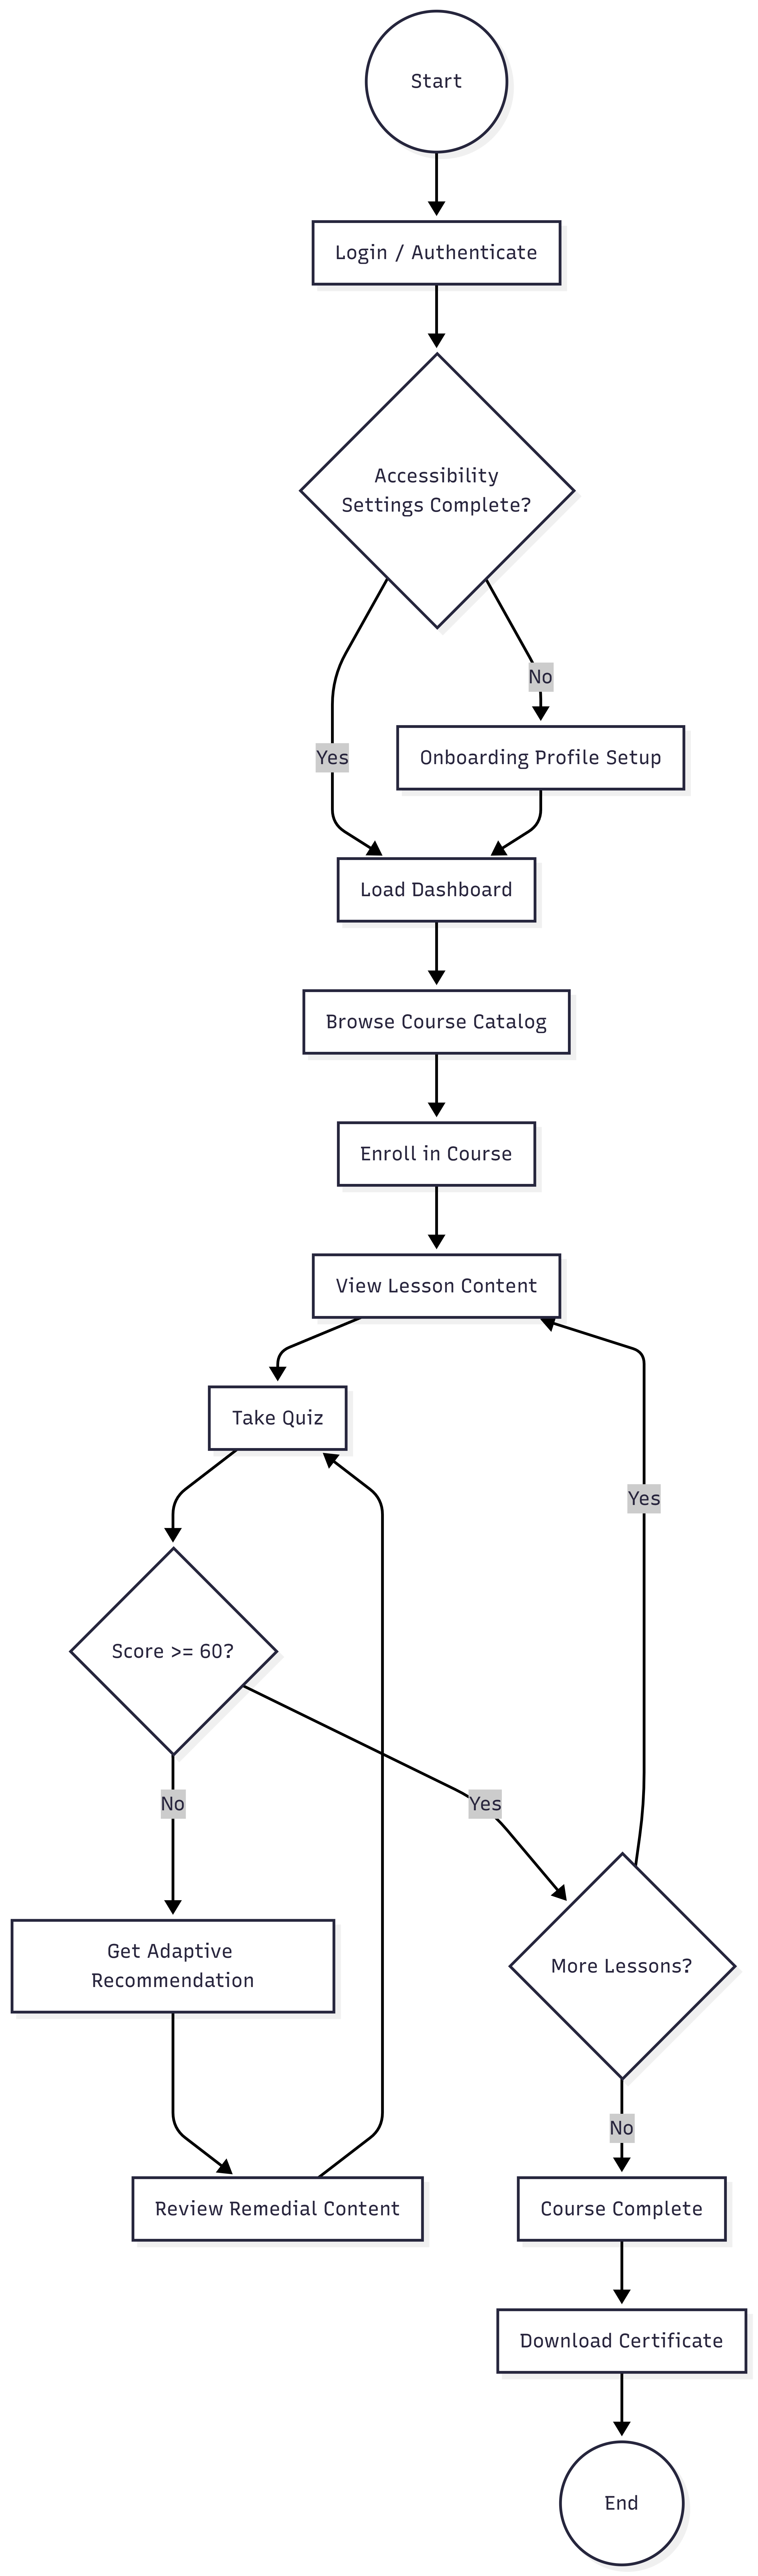
\includegraphics[width=0.55\textwidth,height=0.88\textheight,keepaspectratio]{Diagram/Figure 4.1 Student Activity Diagram.png}
\caption{Learner Activity Diagram}
\label{fig:act_student}
\end{figure}

Figure~\ref{fig:act_student} shows the learner workflow. After the learner signs in, the accessibility module loads the stored settings and applies them before the first page is drawn, so that the learner does not briefly see an unstyled page followed by a correction. A learner with no stored settings is offered a short onboarding step but is not prevented from continuing without it, because an accessibility profile is an aid rather than a requirement.

The main loop consists of browsing the catalogue, enrolling in a course and working through its lessons in order, with progress updated as each lesson is opened and completed. The branch of interest occurs after a quiz. The attempt is graded by the database rather than by the browser. If the score falls below the pass threshold, the recommendation engine records a revision recommendation naming the lesson and the score that produced it. The recommendation is shown prominently but does not lock the learner out of the next lesson, because forcing remediation would turn a support into a penalty for a learner who is already struggling.

\paragraph{Educator workflow}

\begin{figure}[H]
\centering
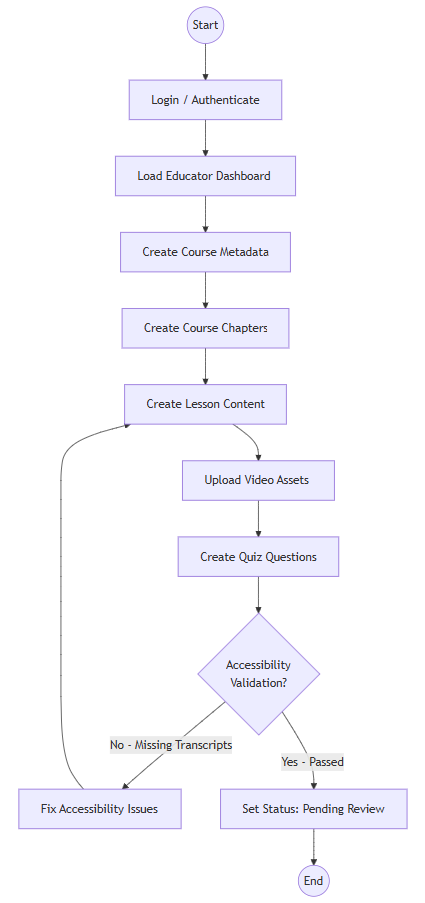
\includegraphics[width=0.75\textwidth,height=0.88\textheight,keepaspectratio]{Diagram/Figure 4.2 Educator Activity Diagram.png}
\caption{Educator Activity Diagram}
\label{fig:act_educator}
\end{figure}

Figure~\ref{fig:act_educator} shows the educator's authoring workflow. It begins with course metadata and, optionally, the chapter structure, and includes one decision that affects everything after it: the primary accessibility focus of the course. That choice determines which rule set the accessibility compliance checker applies to every lesson in the course, so that an educator writing for learners with Dyslexia is checked on sentence length and readability while one writing for autistic learners is checked on figurative language and stated learning objectives.

The educator then enters a content loop of drafting lesson text, embedding media, building activities and writing quiz questions. The compliance checker re-evaluates the draft as it is written, so the accessibility score shown in the editor changes while the lesson is being composed rather than appearing only at the end. When the educator submits the course, its status moves to pending review for administrator moderation. The accessibility check is not a gate in that path: a lesson with unmet standards can still be saved and published, and the panel states this explicitly. The reasoning is given in Section~\ref{sec:a11y-audit}.

\paragraph{Administrator workflow}

\begin{figure}[H]
\centering
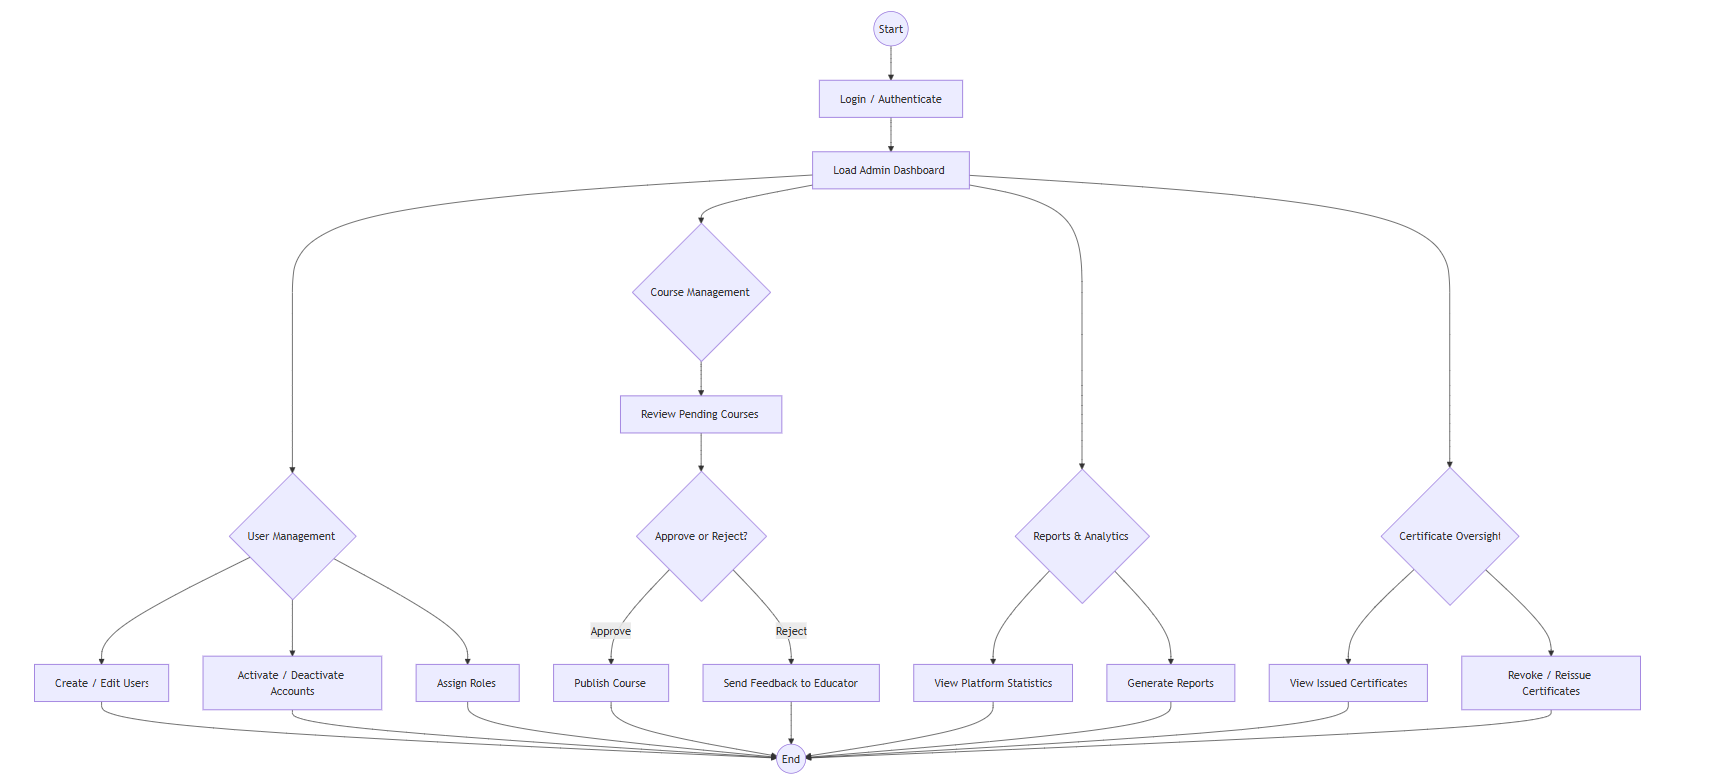
\includegraphics[width=0.75\textwidth,height=0.88\textheight,keepaspectratio]{Diagram/Figure 4.3 Administrator Activity Diagram.png}
\caption{Administrator Activity Diagram}
\label{fig:act_admin}
\end{figure}

The administrator workflow in Figure~\ref{fig:act_admin} is mainly reactive. The administrator monitors two queues: courses awaiting review and applications from users wishing to become educators. When a course enters pending review, the administrator evaluates it, including its course-level accessibility report, and approval publishes the course and notifies the educator. Approving an educator application promotes the applicant, updating both the user record and the authentication account so that the two remain consistent. The remaining administrator activities are oversight rather than moderation: reviewing platform analytics, generating reports, managing user status and handling enquiries submitted through the contact form.

\subsubsection{Interaction Design}

Sequence diagrams show how the components interact over time for four important use cases. One convention runs through all four: an operation drawn as reaching the database directly is one the browser issues under the learner's own session and therefore under row-level security, while an operation drawn as passing through a server route is one that requires privileges the learner does not have. Which of the two is used is a security decision rather than an implementation detail, so the diagrams distinguish them.

\paragraph{Course enrolment}

\begin{figure}[H]
\centering
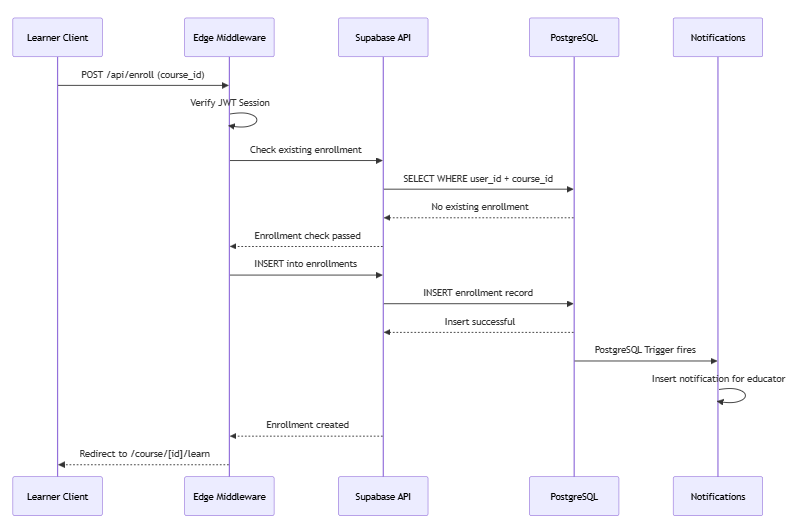
\includegraphics[width=0.75\textwidth,height=0.88\textheight,keepaspectratio]{Diagram/Figure 4.4 Course Enrollment Sequence Diagram.png}
\caption{Course Enrolment Sequence Diagram}
\label{fig:seq_enrollment}
\end{figure}

Figure~\ref{fig:seq_enrollment} shows the enrolment transaction and illustrates how much of the correctness in this architecture is carried by the database rather than by application code.

\begin{enumerate}
    \item The learner selects Enrol on a course page. The request is issued directly to the database under the learner's own session and is therefore evaluated by the database's own access policies.
    \item The insert policy on the enrolment table admits the record only if the learner identified on it is the caller, so a learner cannot enrol anybody else. No application check is required, and none can be bypassed.
    \item A uniqueness rule on the learner and course together prevents a duplicate enrolment. Enrolling again reactivates the existing record instead, which preserves the learner's earlier progress.
    \item A database trigger creates a notification addressed to the educator who owns the course.
    \item The browser returns to the course page, which now shows the lesson roadmap rather than the enrolment prompt.
\end{enumerate}

\paragraph{Lesson viewing and progress}

\begin{figure}[H]
\centering
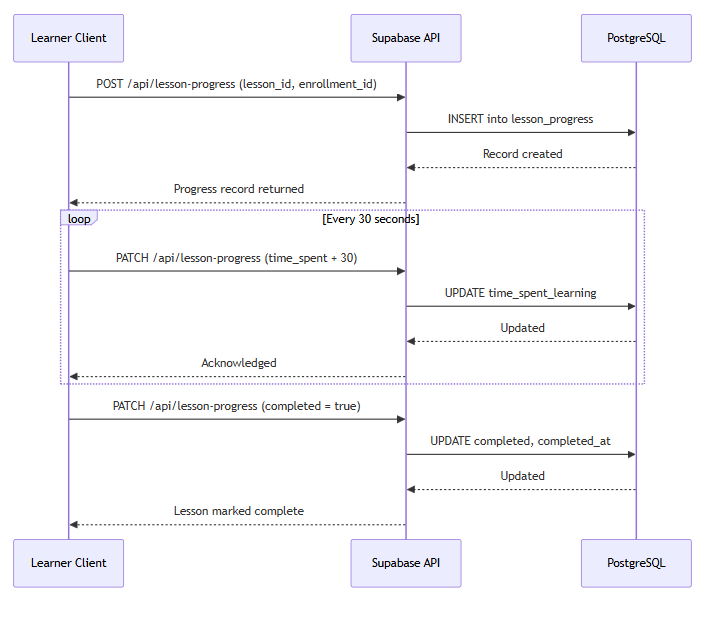
\includegraphics[width=0.75\textwidth,height=0.88\textheight,keepaspectratio]{Diagram/Figure 4.5 Lesson Learning Sequence Diagram.png}
\caption{Lesson Learning Sequence Diagram}
\label{fig:seq_lesson}
\end{figure}

Figure~\ref{fig:seq_lesson} shows how lesson progress is recorded. Opening a lesson creates or updates the learner's progress record, marking the lesson viewed, increasing the view count and recording when it was first opened. While the lesson stays open, the elapsed time is added to that record at intervals rather than only when the page is closed, so that a browser closed abruptly still leaves an accurate record up to the last interval.

Completion is recorded separately from viewing, and the two are kept consistent by a database rule that rejects any progress record marked complete but not viewed. The distinction matters to the recommendation engine, which decides what a learner should do next from completion rather than from viewing; using viewing instead would skip every lesson the learner had merely glanced at.

\paragraph{Quiz attempt and adaptive recommendation}

\begin{figure}[H]
\centering
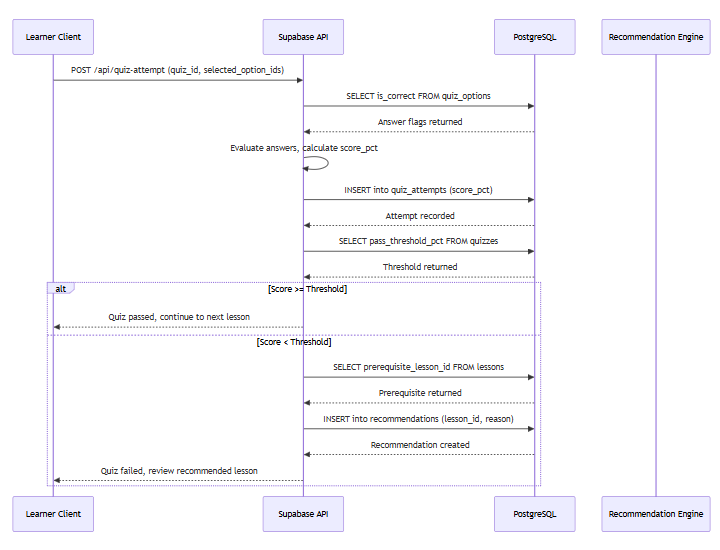
\includegraphics[width=0.75\textwidth,height=0.88\textheight,keepaspectratio]{Diagram/Figure 4.6 Quiz Attempt Sequence Diagram.png}
\caption{Quiz Attempt Sequence Diagram}
\label{fig:seq_quiz}
\end{figure}

Figure~\ref{fig:seq_quiz} shows the most security-sensitive interaction in the system.

\begin{enumerate}
    \item While the learner is answering, the browser reads the answer options through a restricted view that withholds which option is correct for any quiz the learner has not yet submitted. The answer key is therefore not present in the browser at all rather than merely hidden from view.
    \item On submission the browser calls a trusted database function with the quiz identifier and the selected options. It does not calculate a score and does not write the attempt record itself; a database guard would reject such a write.
    \item The function checks that the caller is authenticated and enrolled in the course, and refuses the attempt if the quiz's attempt limit has been reached.
    \item It grades each answer against the stored correct option, records the attempt and its answers, and evaluates the result against the pass threshold. It returns the score, the pass decision and the threshold used, so that the interface can explain the result rather than only report it.
    \item A database trigger raises a notification for the educator.
    \item The answer key becomes readable to that learner for that quiz, which is what allows the review screen to show which answers were wrong.
    \item The recommendation engine records a revision recommendation for the lesson, carrying the score that produced it as its stated reason.
\end{enumerate}

\paragraph{Course creation and media upload}

\begin{figure}[H]
\centering
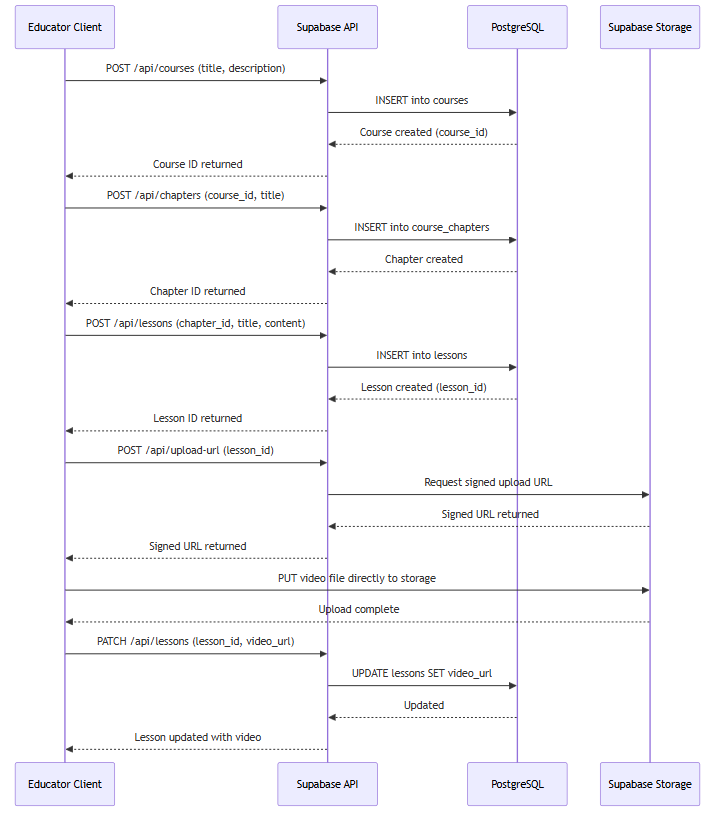
\includegraphics[width=0.75\textwidth,height=0.88\textheight,keepaspectratio]{Diagram/Figure 4.7 Course Creation Sequence Diagram.png}
\caption{Course Creation Sequence Diagram}
\label{fig:seq_course_creation}
\end{figure}

Figure~\ref{fig:seq_course_creation} shows the authoring pipeline. Lesson text is composed in the rich-text editor, sanitised and saved to the lesson, with a snapshot added to the version history so that an edit can be undone later. Images and documents are uploaded from the browser directly into cloud storage, so that a large file does not have to pass through the application server, and the resulting address is recorded against the course.

Instructional video is handled differently. It is embedded from an external host by address rather than uploaded, so the lesson holds only a reference to a resource the platform does not store or serve. Throughout this pipeline the accessibility compliance checker re-runs on every change, so the accessibility consequence of an edit, such as adding a video without a transcript, is visible at the moment the edit is made rather than at publication.

\subsubsection{User Interface Design}
\label{sec:ui-design}
\setcounter{uidsub}{0}

The interface is organised into three role-specific shells, each with its own navigation, input surfaces and outputs. Every figure in this section is a screenshot of the running system taken against the reproducible demonstration database described in Section~\ref{sec:phys-db}.

\uidesignsub{Navigation Design}

Navigation follows a role-based shell pattern. The area of the site a user reaches determines the shell, and a server-side check refuses a shell the signed-in role is not entitled to before the page is rendered.

\begin{itemize}
    \item \textbf{Public navigation.} Visitors who are not signed in can reach the landing page, login, sign-up, password recovery, the contact form, the educator application form and the published accessibility statement. Certificate verification is also public, so that a third party can check a certificate without an account.
    \item \textbf{Learner shell.} A sidebar carries Dashboard, My Courses, Progress, Achievements and Certificates, and Accessibility. A top bar holds the notification indicator and the profile menu. Two properties of this sidebar are deliberate. Every item is a real hyperlink rather than a click handler, so that a screen reader announces navigation as navigation and the browser's own behaviour such as opening a link in a new tab continues to work. The sidebar also responds to the accessibility preset: the Dyslexia preset widens it and enlarges its text, and the distraction-free presets remove it entirely while a lesson is open.
    \item \textbf{Educator shell.} A sidebar carries Dashboard, Courses, Educator Ranking, Analytics, Learner Progress and Certificates. Inside a course, a tab bar provides Overview, Lessons, Assets, Learners, Certificates, Achievements and Settings.
    \item \textbf{Administrator shell.} A sidebar carries Dashboard, User Management, Course Management, Educator Applications, Feedback, Certificates, Analytics and Reports.
\end{itemize}

Figure~\ref{fig:ui_learner_dashboard} shows the learner dashboard with no accessibility preset applied, and Figure~\ref{fig:ui_edu_workspace} shows the corresponding educator course workspace with the tab bar, the ordered lesson list and the per-lesson authoring controls.

\begin{figure}[htbp]
\centering
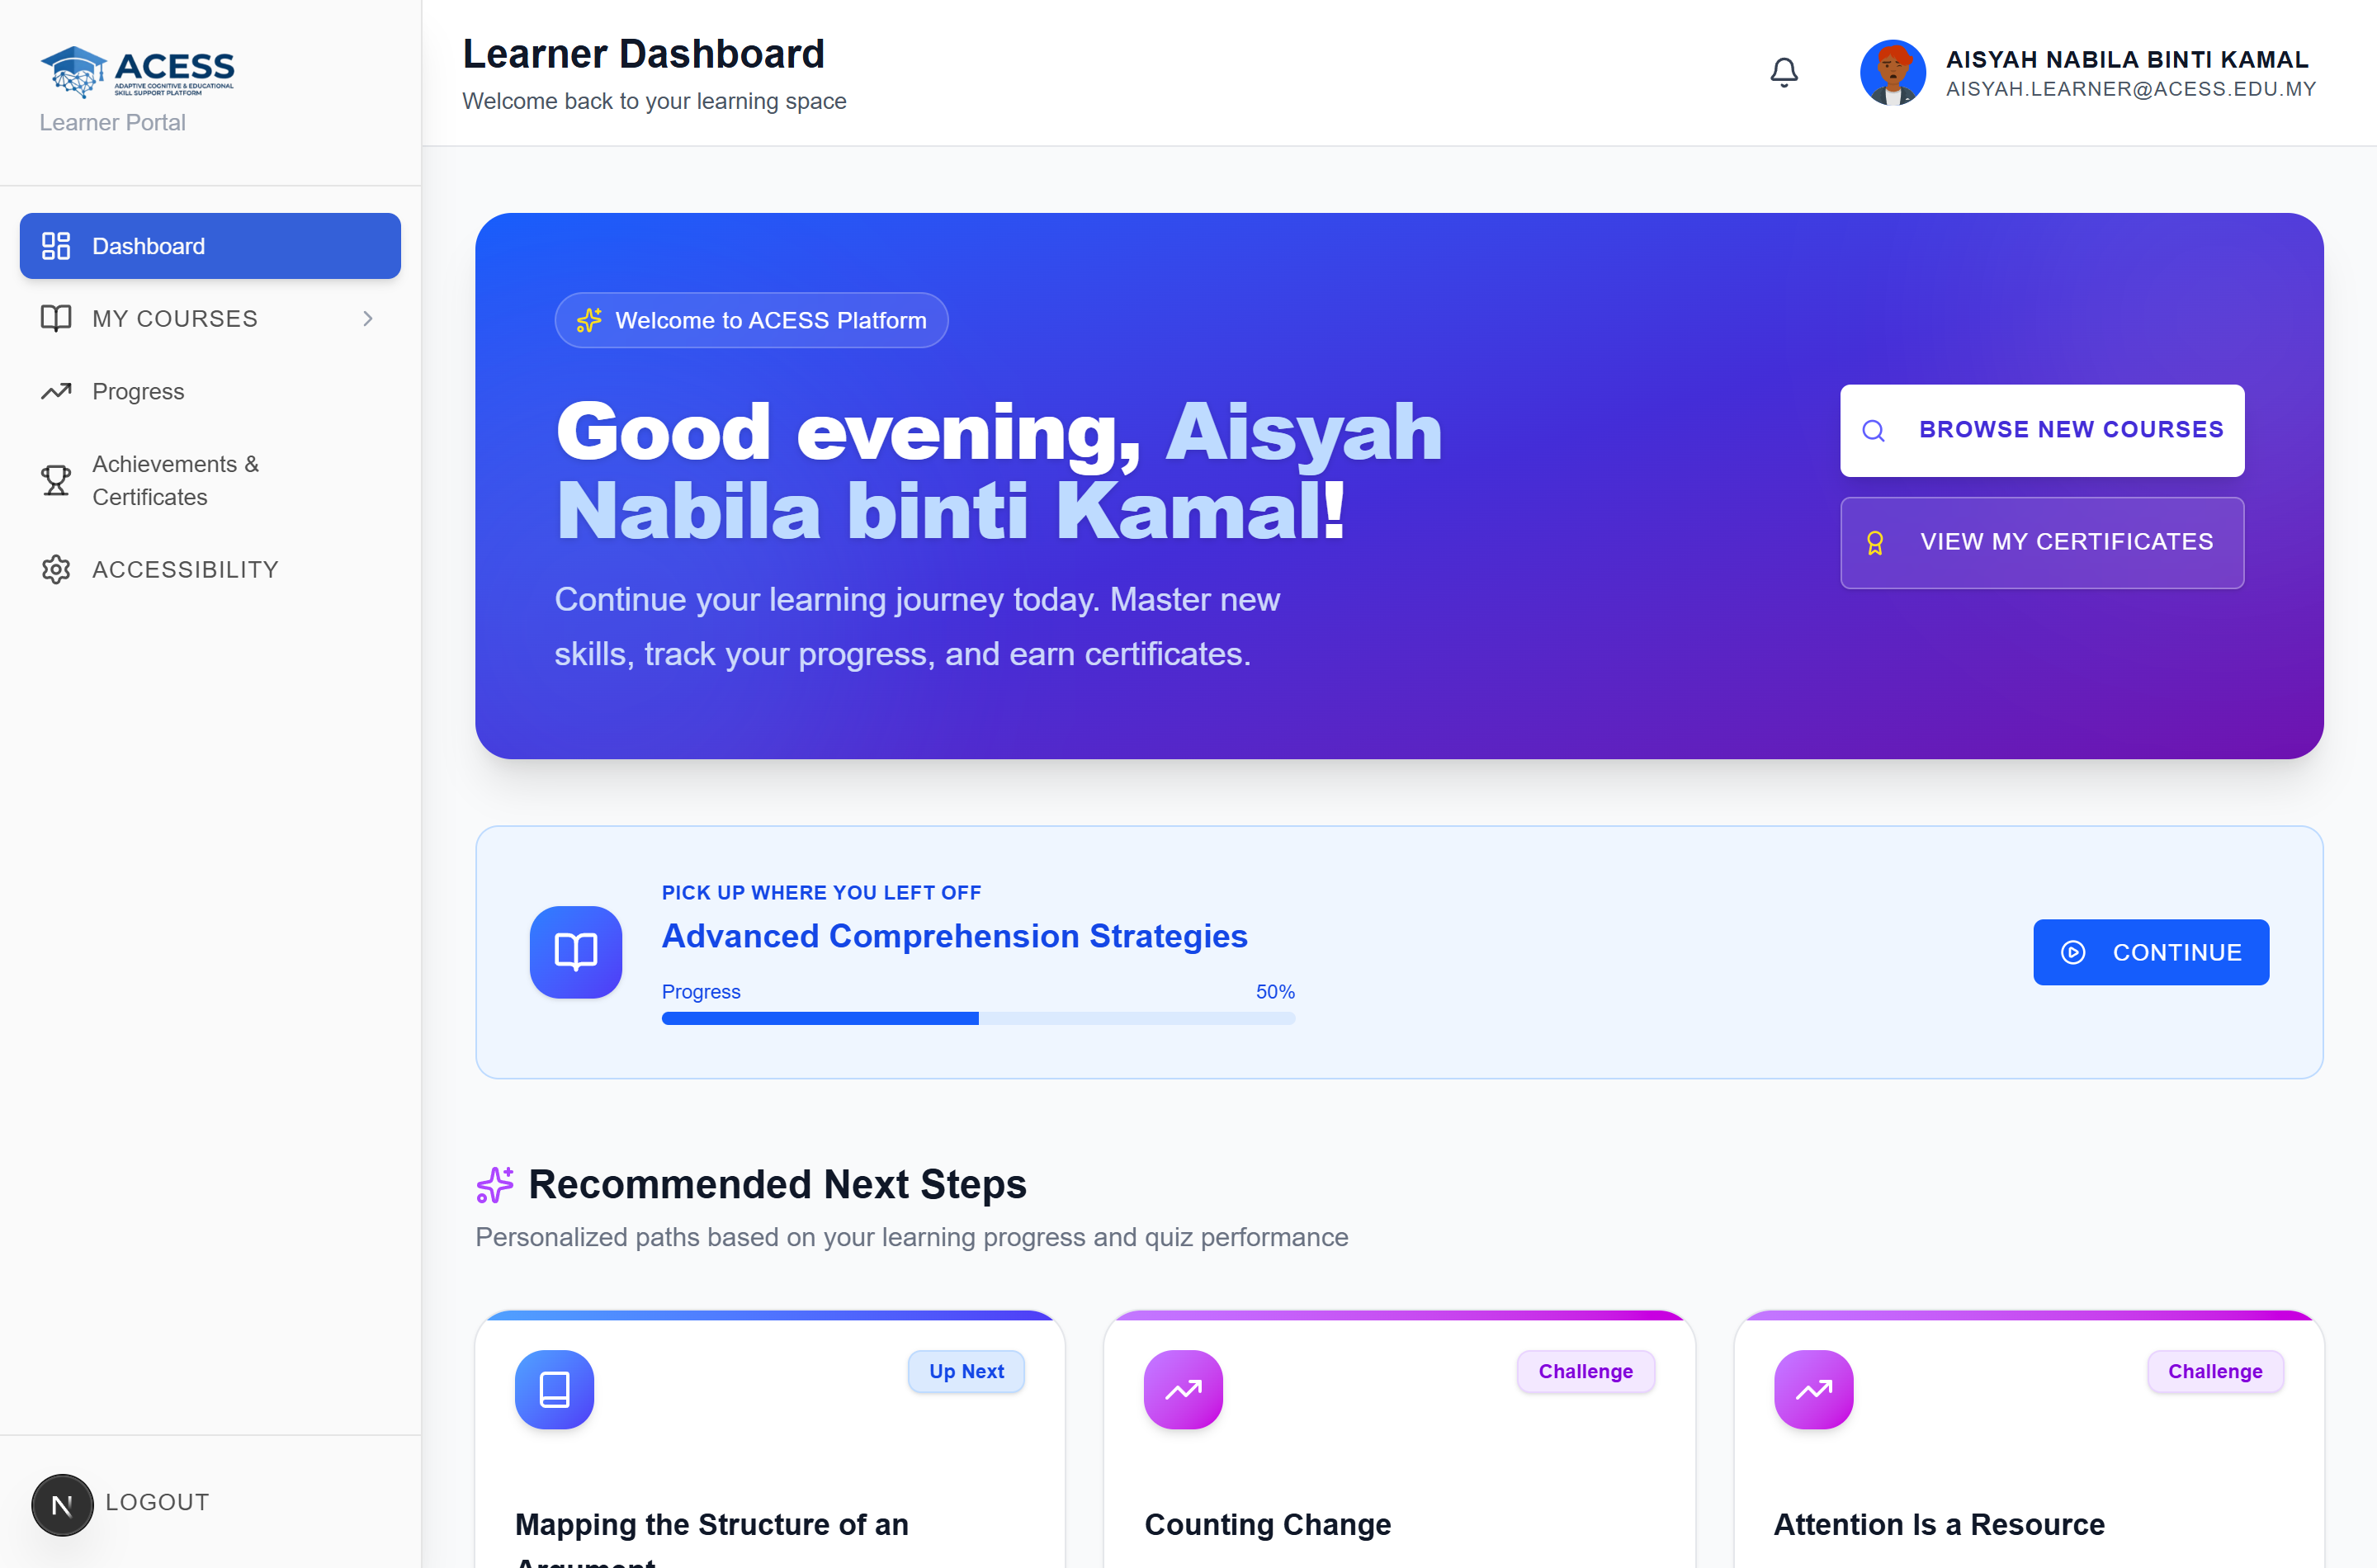
\includegraphics[width=0.92\textwidth]{Screenshots/dashboard-none.png}
\caption{Learner Dashboard in the Default State}
\label{fig:ui_learner_dashboard}
\end{figure}

\begin{figure}[htbp]
\centering
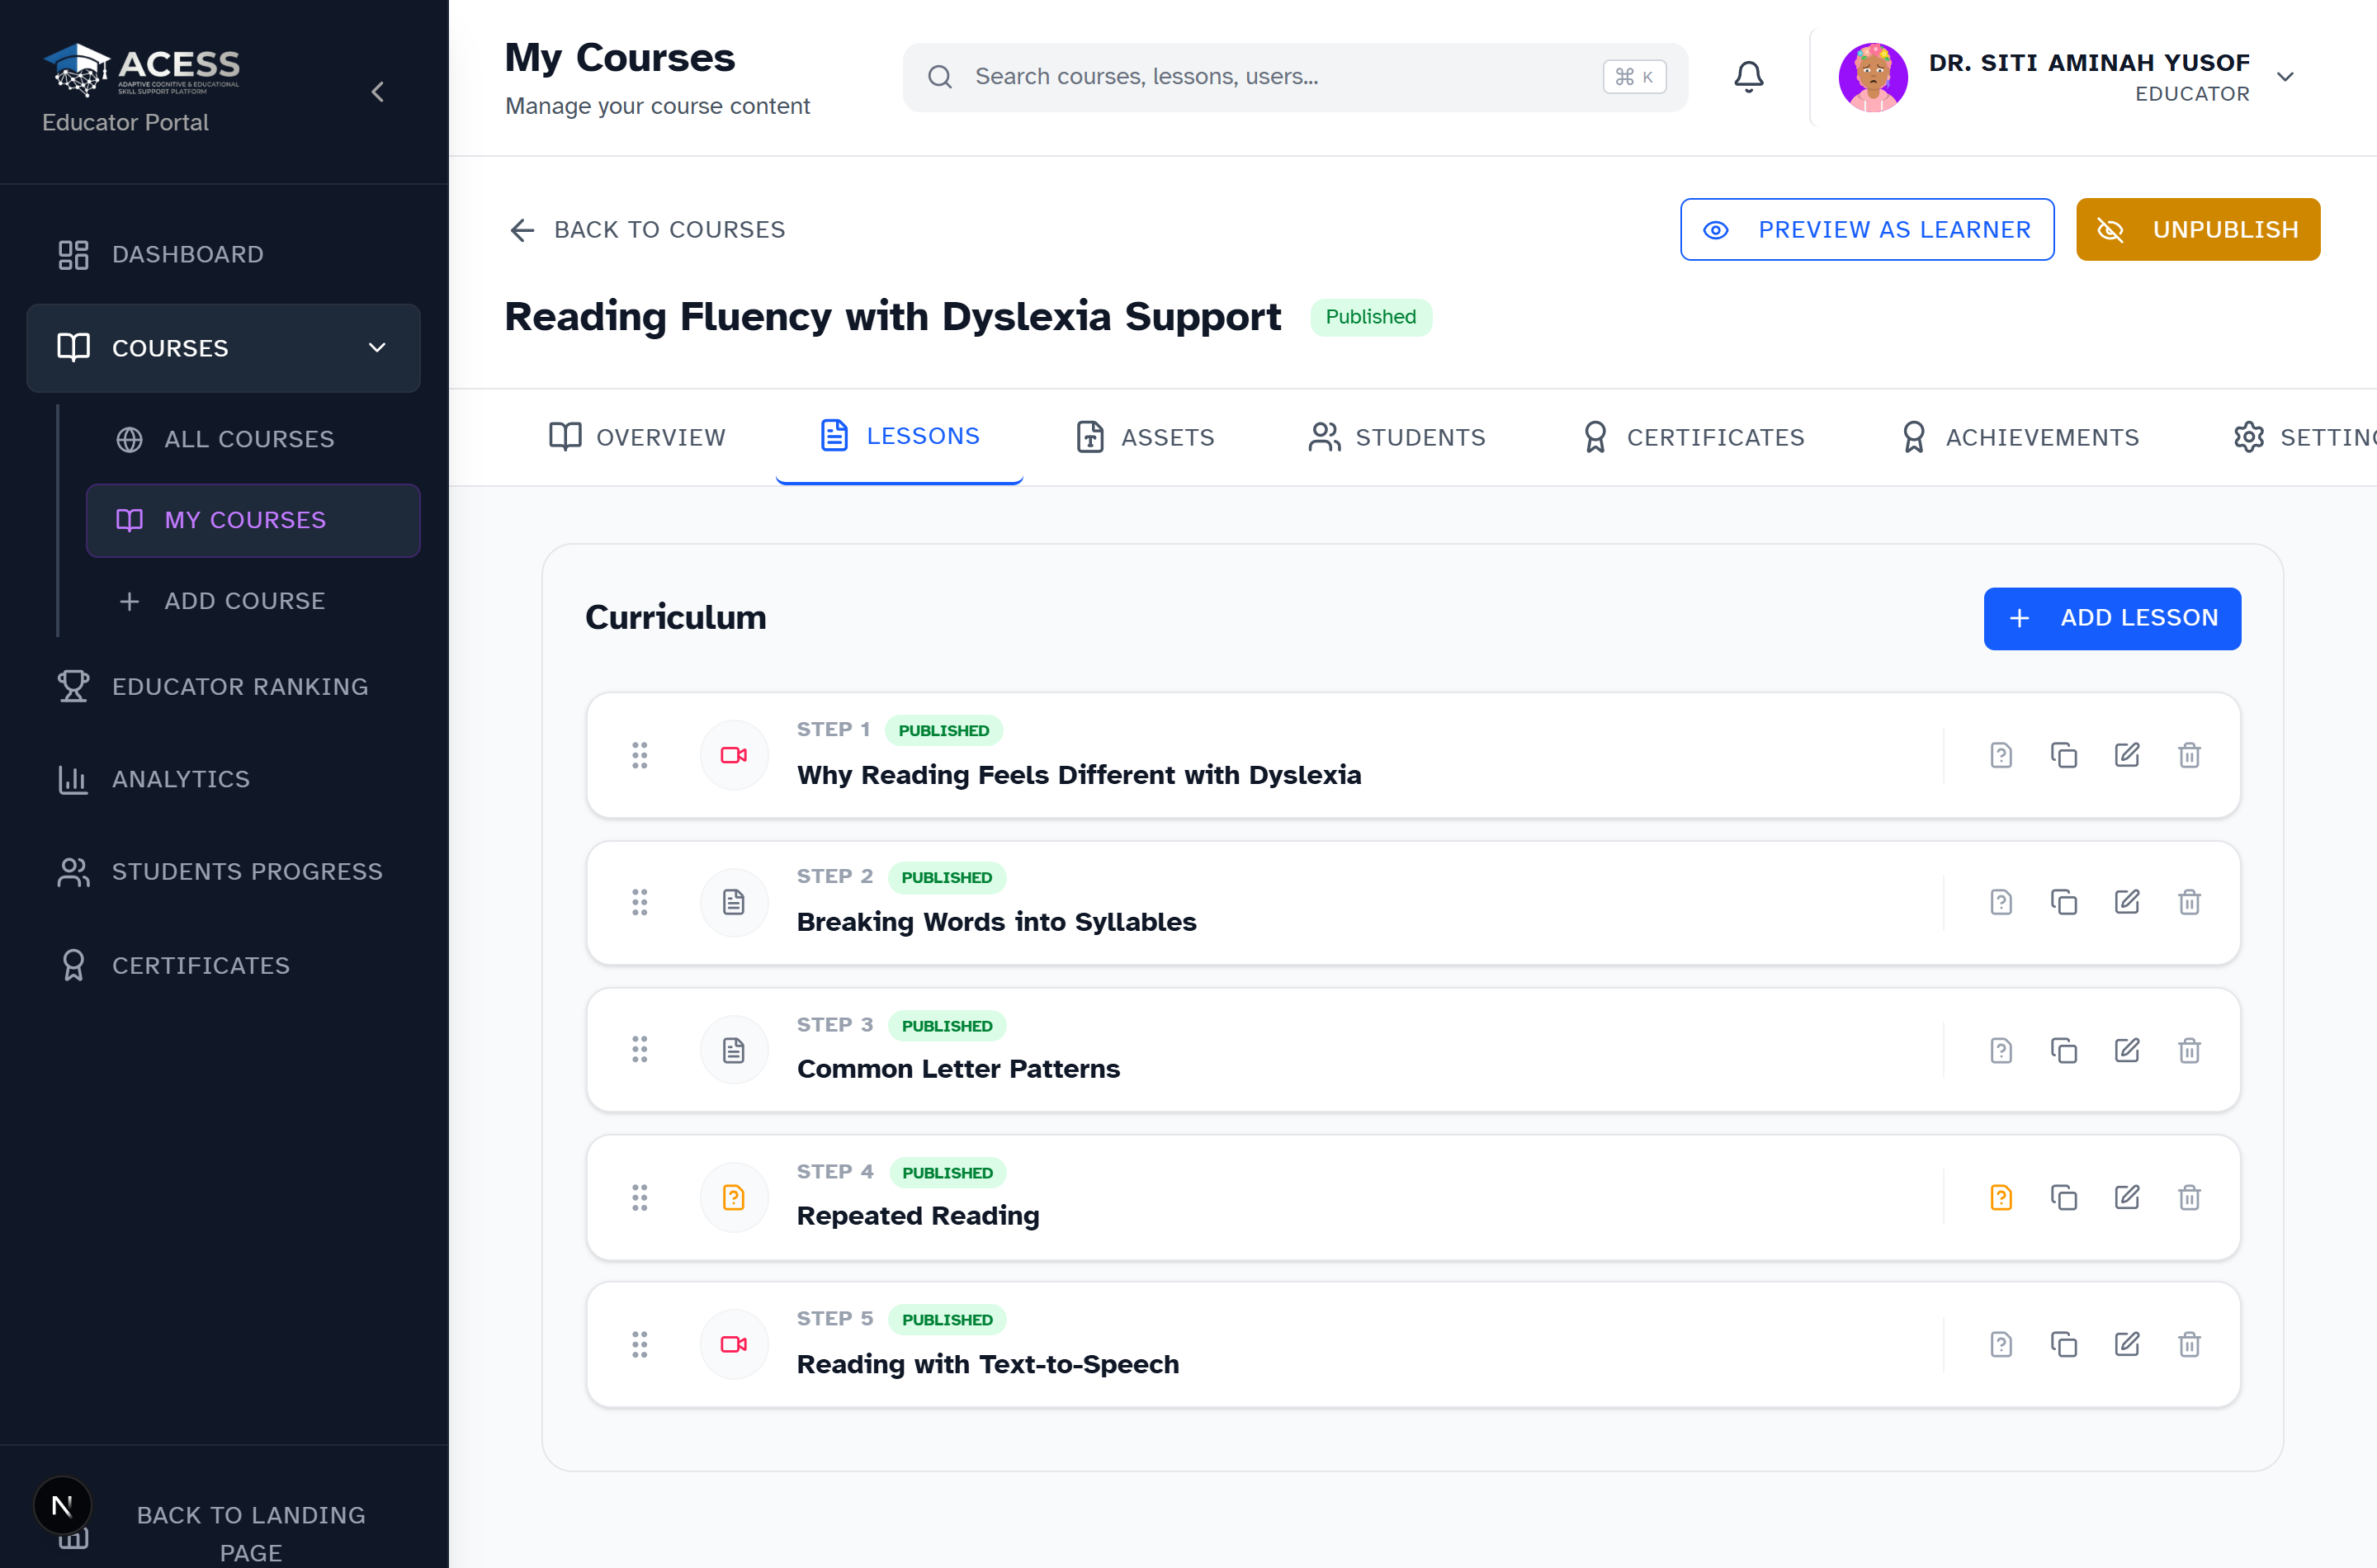
\includegraphics[width=0.92\textwidth]{Screenshots/educator-course-workspace.png}
\caption{Educator Course Workspace, Lessons Tab}
\label{fig:ui_edu_workspace}
\end{figure}

\uidesignsub{Input Design}

The input surfaces of the system are grouped below by the role that uses them.

\begin{itemize}
    \item \textbf{Public input.} A visitor supplies an email address and password at sign-up, and a category, subject and message on the contact form. A requested role is never accepted from the sign-up request itself: self-registration is always fixed to the learner role by the database.
    \item \textbf{Learner input.} A learner selects a course to enrol in, adjusts accessibility settings such as text size and line spacing from the accessibility panel shown in Figure~\ref{fig:ui_a11y_modal}, answers quiz questions as shown in Figure~\ref{fig:ui_quiz}, and uploads a profile picture.
    \item \textbf{Educator input.} An educator supplies course metadata such as title, address, difficulty and status, writes lesson content in the rich-text editor, sets the order and layout of each lesson, and creates quiz questions and their answer options.
    \item \textbf{Administrator input.} An administrator sets a user's role, decides whether a submitted course is approved or rejected, and selects the date range for a platform report.
\end{itemize}

Table~\ref{tab:input_validation} states the validation rule applied to each significant field and the layer at which it is enforced. The distinction matters, because a rule enforced only in the browser is a convenience, whereas a rule enforced by a database constraint or an access policy cannot be bypassed by a crafted request.

{
\renewcommand{\arraystretch}{1.2}
\setstretch{1.05}
\footnotesize
\begin{longtable}{|>{\raggedright\arraybackslash\tabbreak}p{2.43cm}|>{\raggedright\arraybackslash\tabbreak}p{2.89cm}|>{\raggedright\arraybackslash\tabbreak}p{4.29cm}|>{\raggedright\arraybackslash\tabbreak}p{3.17cm}|}
\caption{Input Validation Rules}
\label{tab:input_validation}\\
\hline
\textbf{Screen} & \textbf{Field} & \textbf{Validation rule} & \textbf{Enforced at} \\
\hline \hline
\endfirsthead
\multicolumn{4}{l}{\footnotesize\itshape Table~\ref{tab:input_validation} continued from the previous page}\\
\hline
\textbf{Screen} & \textbf{Field} & \textbf{Validation rule} & \textbf{Enforced at} \\
\hline \hline
\endhead
\hline
\multicolumn{4}{r}{\footnotesize\itshape continued on the next page}\\
\endfoot
\endlastfoot
Sign up & Email & Well-formed address, must be unique & Browser, then authentication service \\ \hline
Sign up & Password & Minimum length and complexity & Browser, then authentication service \\ \hline
Sign up & Role & Always learner, not accepted from the request & Database trigger \\ \hline
Course form & Title & Required, must not be blank & Browser and database \\ \hline
Course form & Address & Unique across all courses & Database constraint \\ \hline
Course form & Difficulty & One of beginner, intermediate or advanced & Database constraint \\ \hline
Course form & Status & One of draft, pending review, published or archived & Database constraint \\ \hline
Lesson editor & Rich text & Sanitised before display, disallowed markup removed & Browser sanitiser \\ \hline
Lesson editor & Sequence order & Integer greater than zero & Database constraint \\ \hline
Lesson editor & Lesson layout & One of the five permitted layouts & Database constraint \\ \hline
Quiz builder & Pass threshold & Integer between 0 and 100 & Database constraint \\ \hline
Quiz builder & Answer options & At least two options, exactly one correct & Browser \\ \hline
Quiz attempt & Selected options & Graded on the server, answer key not sent early & Database function and view \\ \hline
Accessibility panel & Text size & Between 12 and 24\,px & Browser \\ \hline
Accessibility panel & Line spacing & Between 1.0 and 3.0 & Browser \\ \hline
Enrolment & Course reference & A learner may only enrol themselves & Access policy \\ \hline
Enrolment & Status & One of active, completed or dropped; completion cannot be set by the browser & Database constraint and guard \\ \hline
Contact form & Category & One of five permitted categories & Database constraint \\ \hline
Profile picture & File location & Must sit inside the uploader's own folder & Storage policy \\ \hline
\end{longtable}
}

The most important input surface in the system is the accessibility panel shown in Figure~\ref{fig:ui_a11y_modal}. It presents four preset buttons above five grouped tabs (Reading, Focus, Sensory, Supports and Profile), and every control is saved to the learner's settings and takes effect without reloading the page.

\begin{figure}[htbp]
\centering
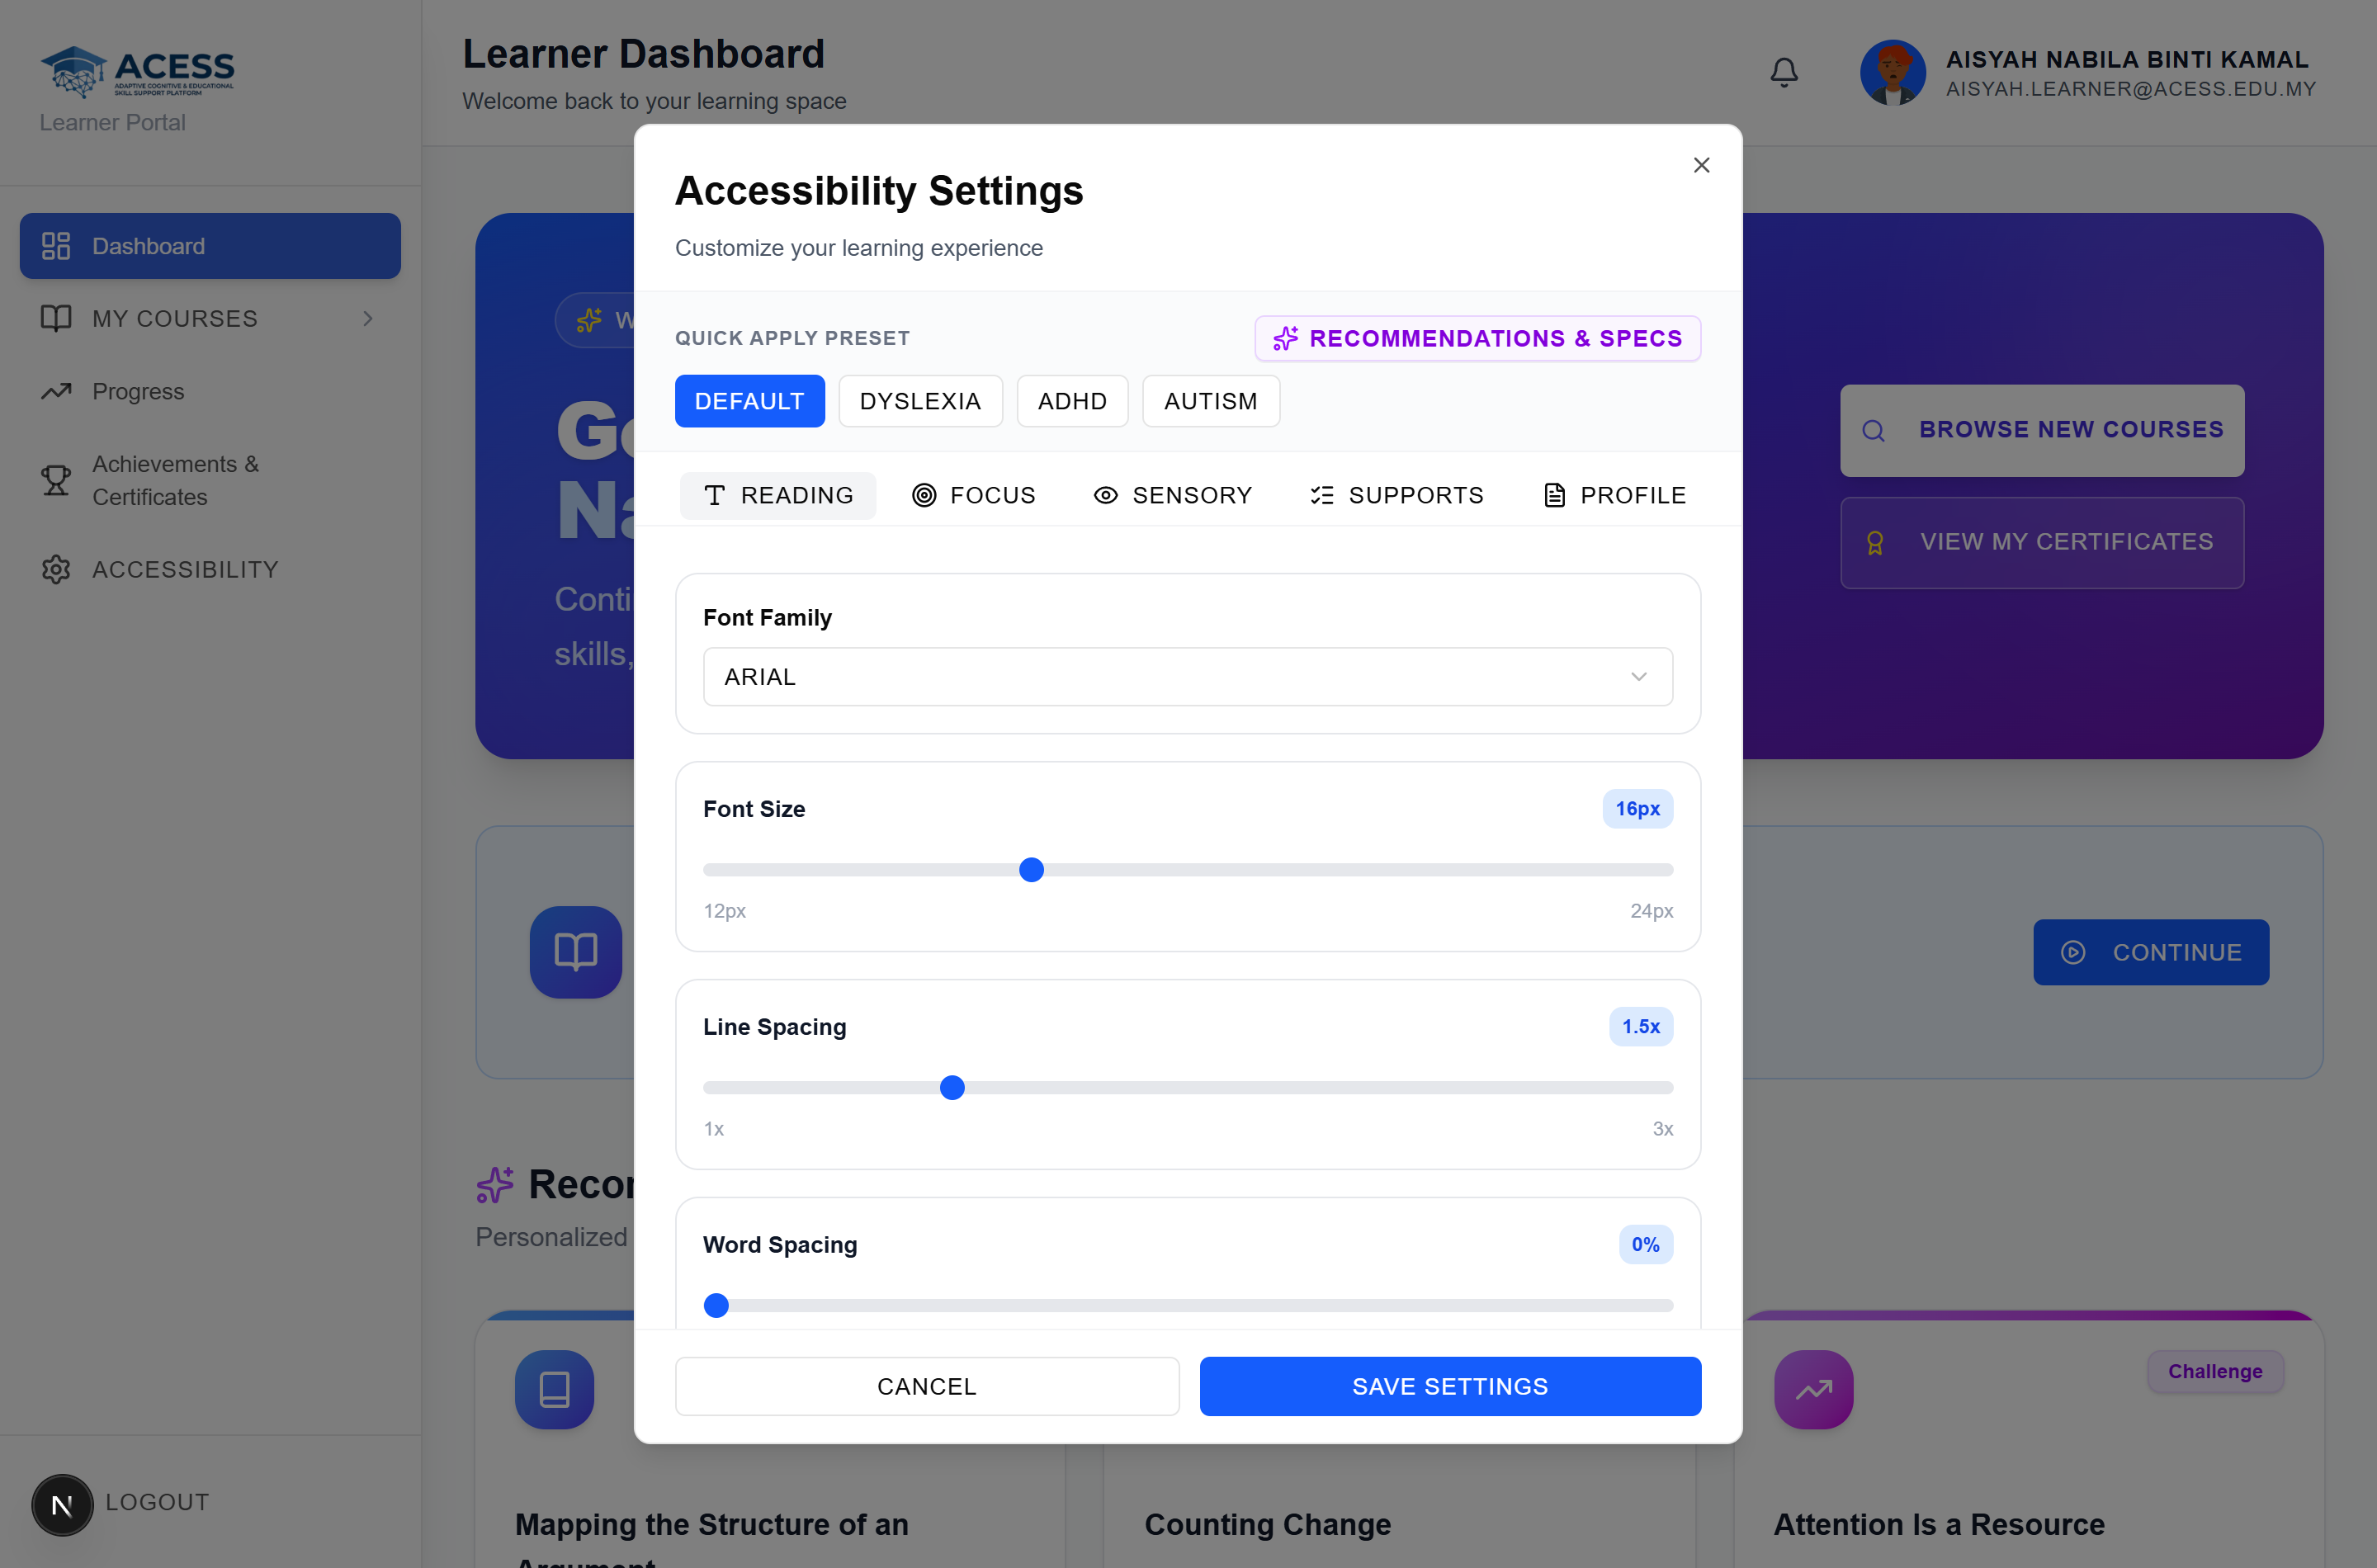
\includegraphics[width=0.92\textwidth]{Screenshots/a11y-settings-modal.png}
\caption{Accessibility Settings Panel, Reading Group}
\label{fig:ui_a11y_modal}
\end{figure}

The second significant input surface is the quiz shown in Figure~\ref{fig:ui_quiz}. Its design carries three accessibility decisions: questions are presented one per screen regardless of the lesson's own layout setting, a time limit set by the educator is displayed to the learner, and the conditions of the attempt are stated before it begins rather than discovered during it.

\begin{figure}[htbp]
\centering
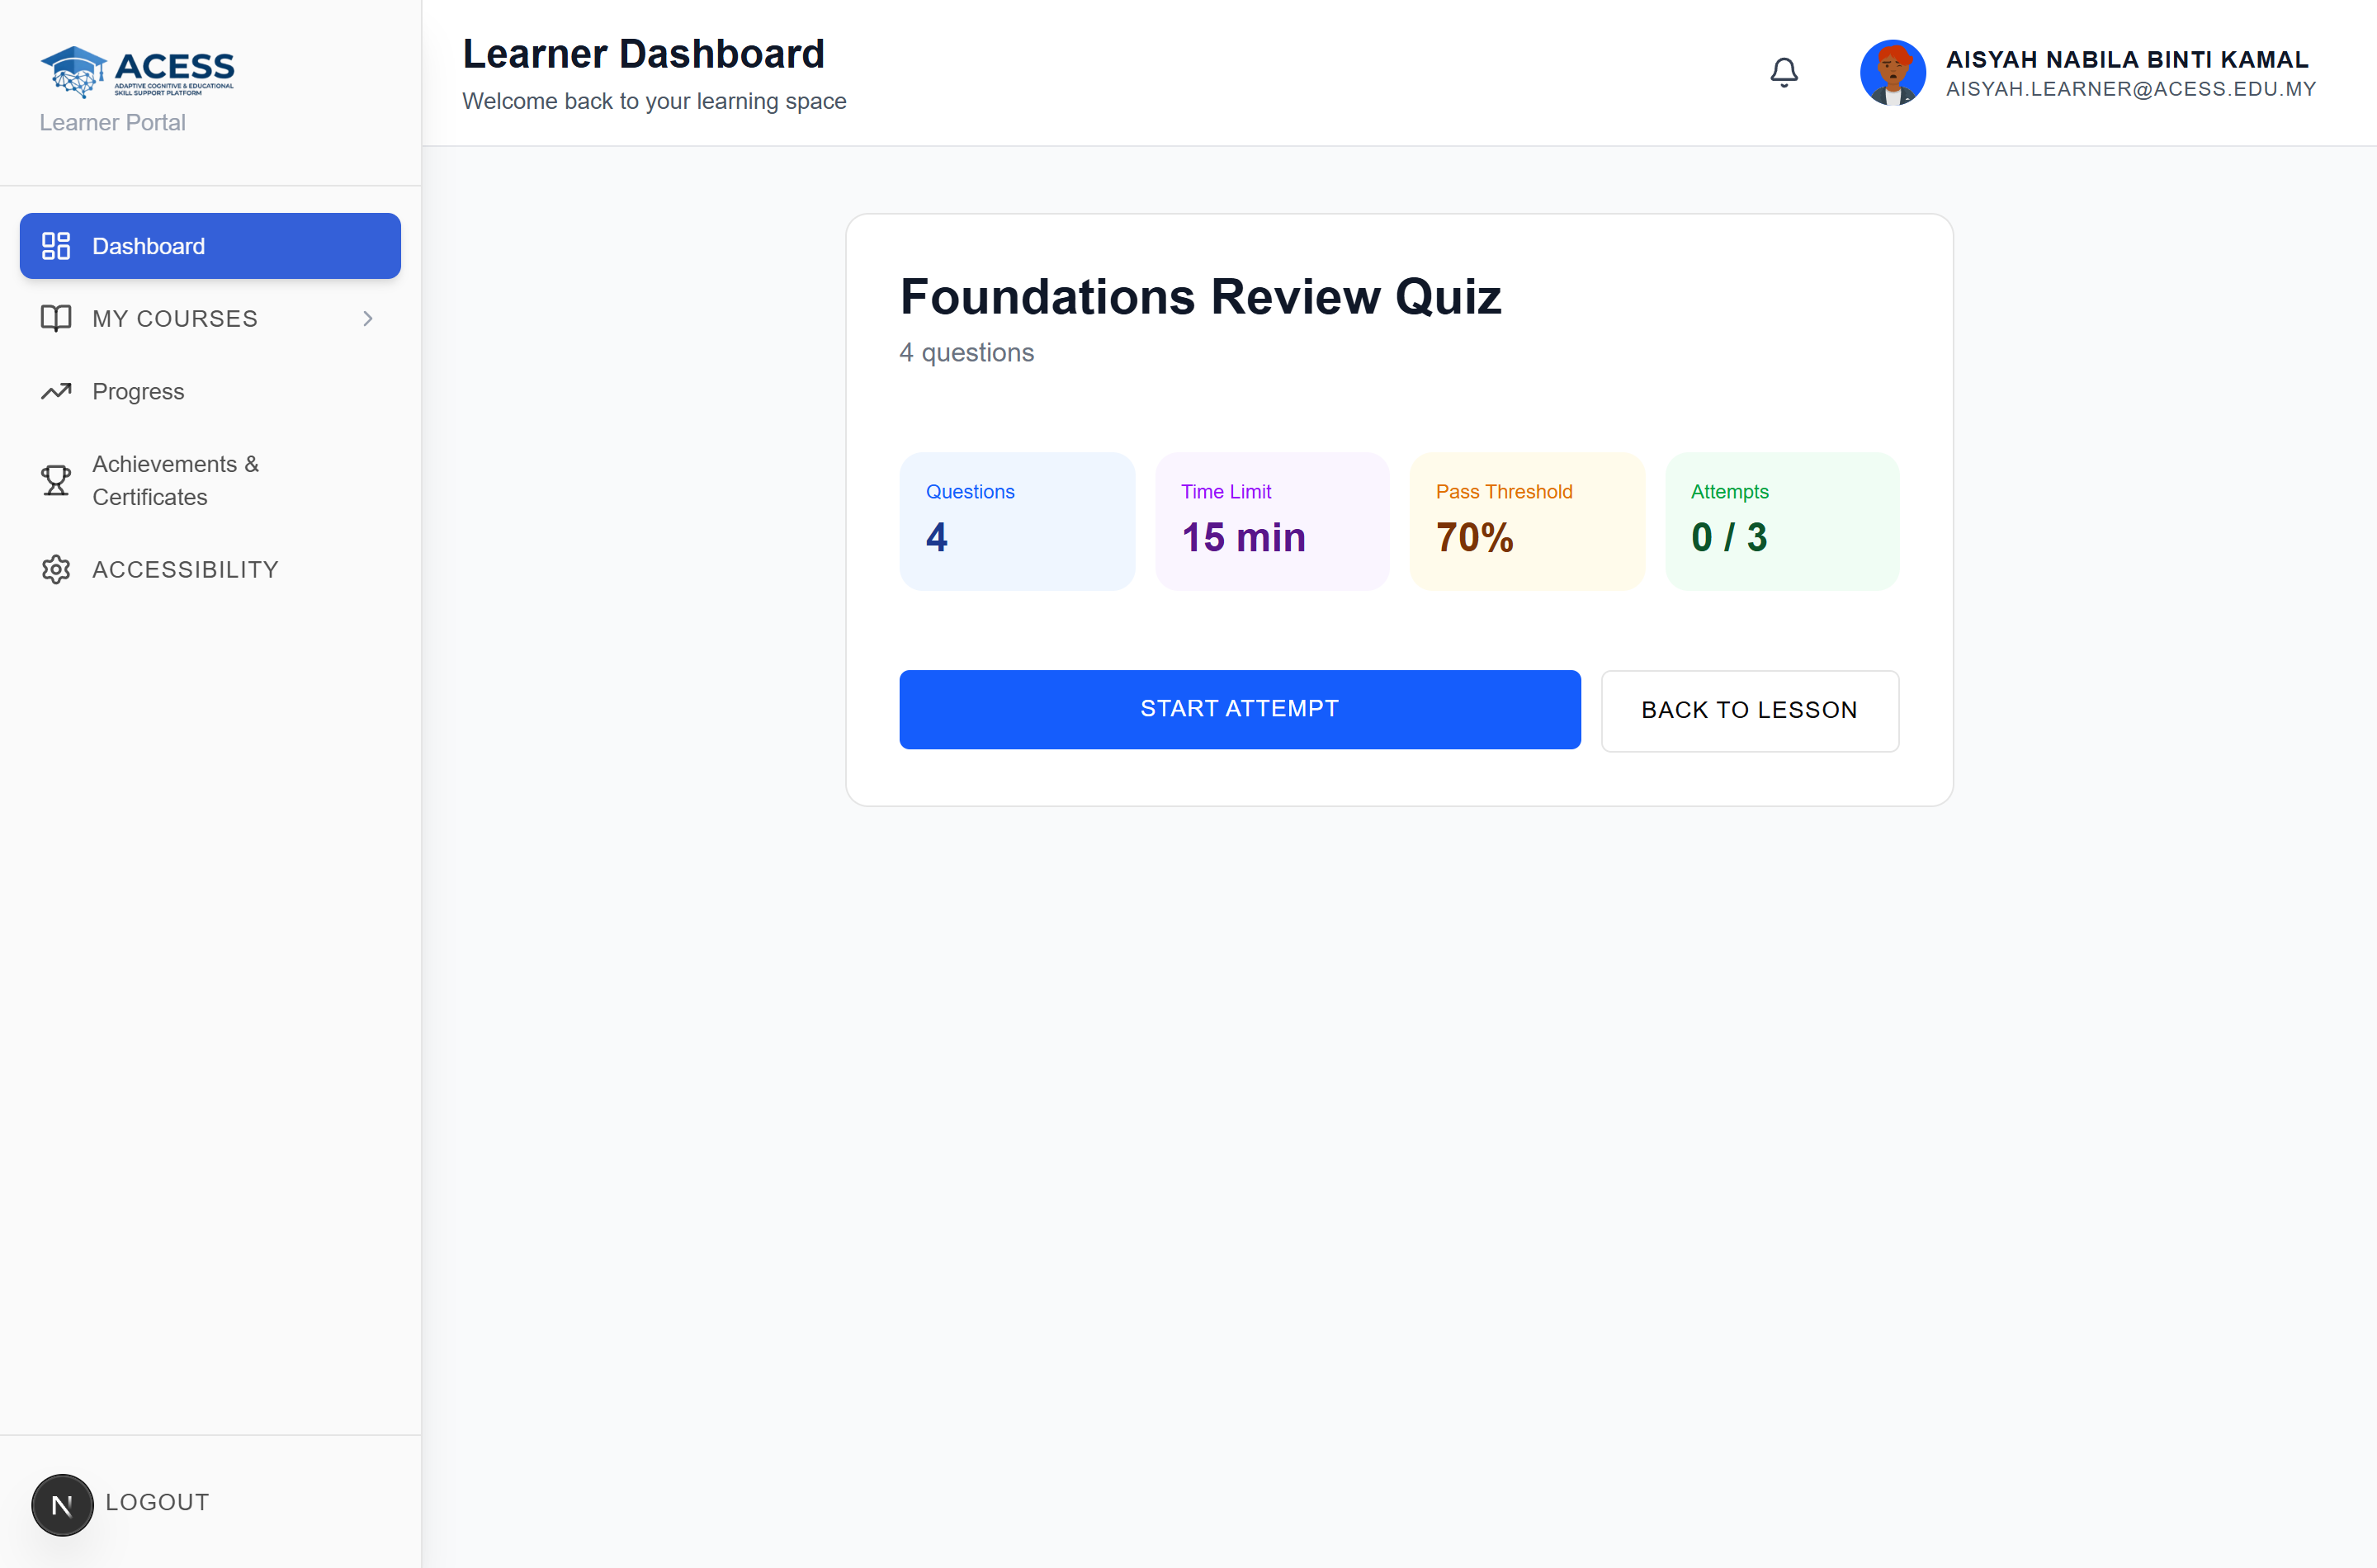
\includegraphics[width=0.92\textwidth]{Screenshots/learner-quiz.png}
\caption{Quiz Interface}
\label{fig:ui_quiz}
\end{figure}

\uidesignsub{Output Design}

Outputs fall into three classes: screen output produced on demand, document output produced on demand, and output raised automatically by an event. Table~\ref{tab:output_design} classifies every output by its basis, its audience and its content.

\begin{table}[H]
\caption{System Outputs}
\label{tab:output_design}
\vspace{-4mm}
\begin{center}
\renewcommand{\arraystretch}{1.2}
\setstretch{1.05}
\footnotesize
\begin{tabular}{|>{\raggedright\arraybackslash\tabbreak}p{3.32cm}|>{\raggedright\arraybackslash\tabbreak}p{1.99cm}|>{\raggedright\arraybackslash\tabbreak}p{2.0cm}|>{\raggedright\arraybackslash\tabbreak}p{5.59cm}|}
\hline
\textbf{Output} & \textbf{Basis} & \textbf{Audience} & \textbf{Content} \\
\hline \hline
Learner progress page & On demand & Learner & Course completion, lessons completed, study time, quiz history, visit history \\ \hline
Course analytics & On demand & Educator & Enrolment and completion trends, per-lesson completion, quiz score distribution, at-risk flags \\ \hline
Platform analytics & On demand & Administrator & Registrations, enrolments, learning time, accessibility feature use and preset adoption \\ \hline
Accessibility compliance report & Continuous & Educator & Per-lesson and per-course score, unmet rules, the source of each rule \\ \hline
Administrator report (PDF) & On demand & Administrator & Platform, course, learner or content-coverage report over a chosen date range \\ \hline
Completion certificate (PDF) & Event & Learner & Learner name, course, completion date, reference code, verification QR code \\ \hline
Certificate verification page & On demand & Public & Validity, issue date and revocation status for a reference code \\ \hline
Notifications & Event & All roles & Enrolment, lesson progress, quiz attempt, lesson added, course published \\ \hline
Achievement award & Event & Learner & Badge unlocked when a course achievement requirement is met \\ \hline
\end{tabular}
\end{center}
\end{table}

Figure~\ref{fig:ui_learner_progress} shows the learner progress page, with completion, study time and quiz history for the signed-in learner, and Figure~\ref{fig:ui_admin_analytics} shows the administrator equivalent with platform-level summary tiles and the registration trend. Both use the same charting library, so that a chart carries the same visual conventions wherever it appears.

\begin{figure}[htbp]
\centering
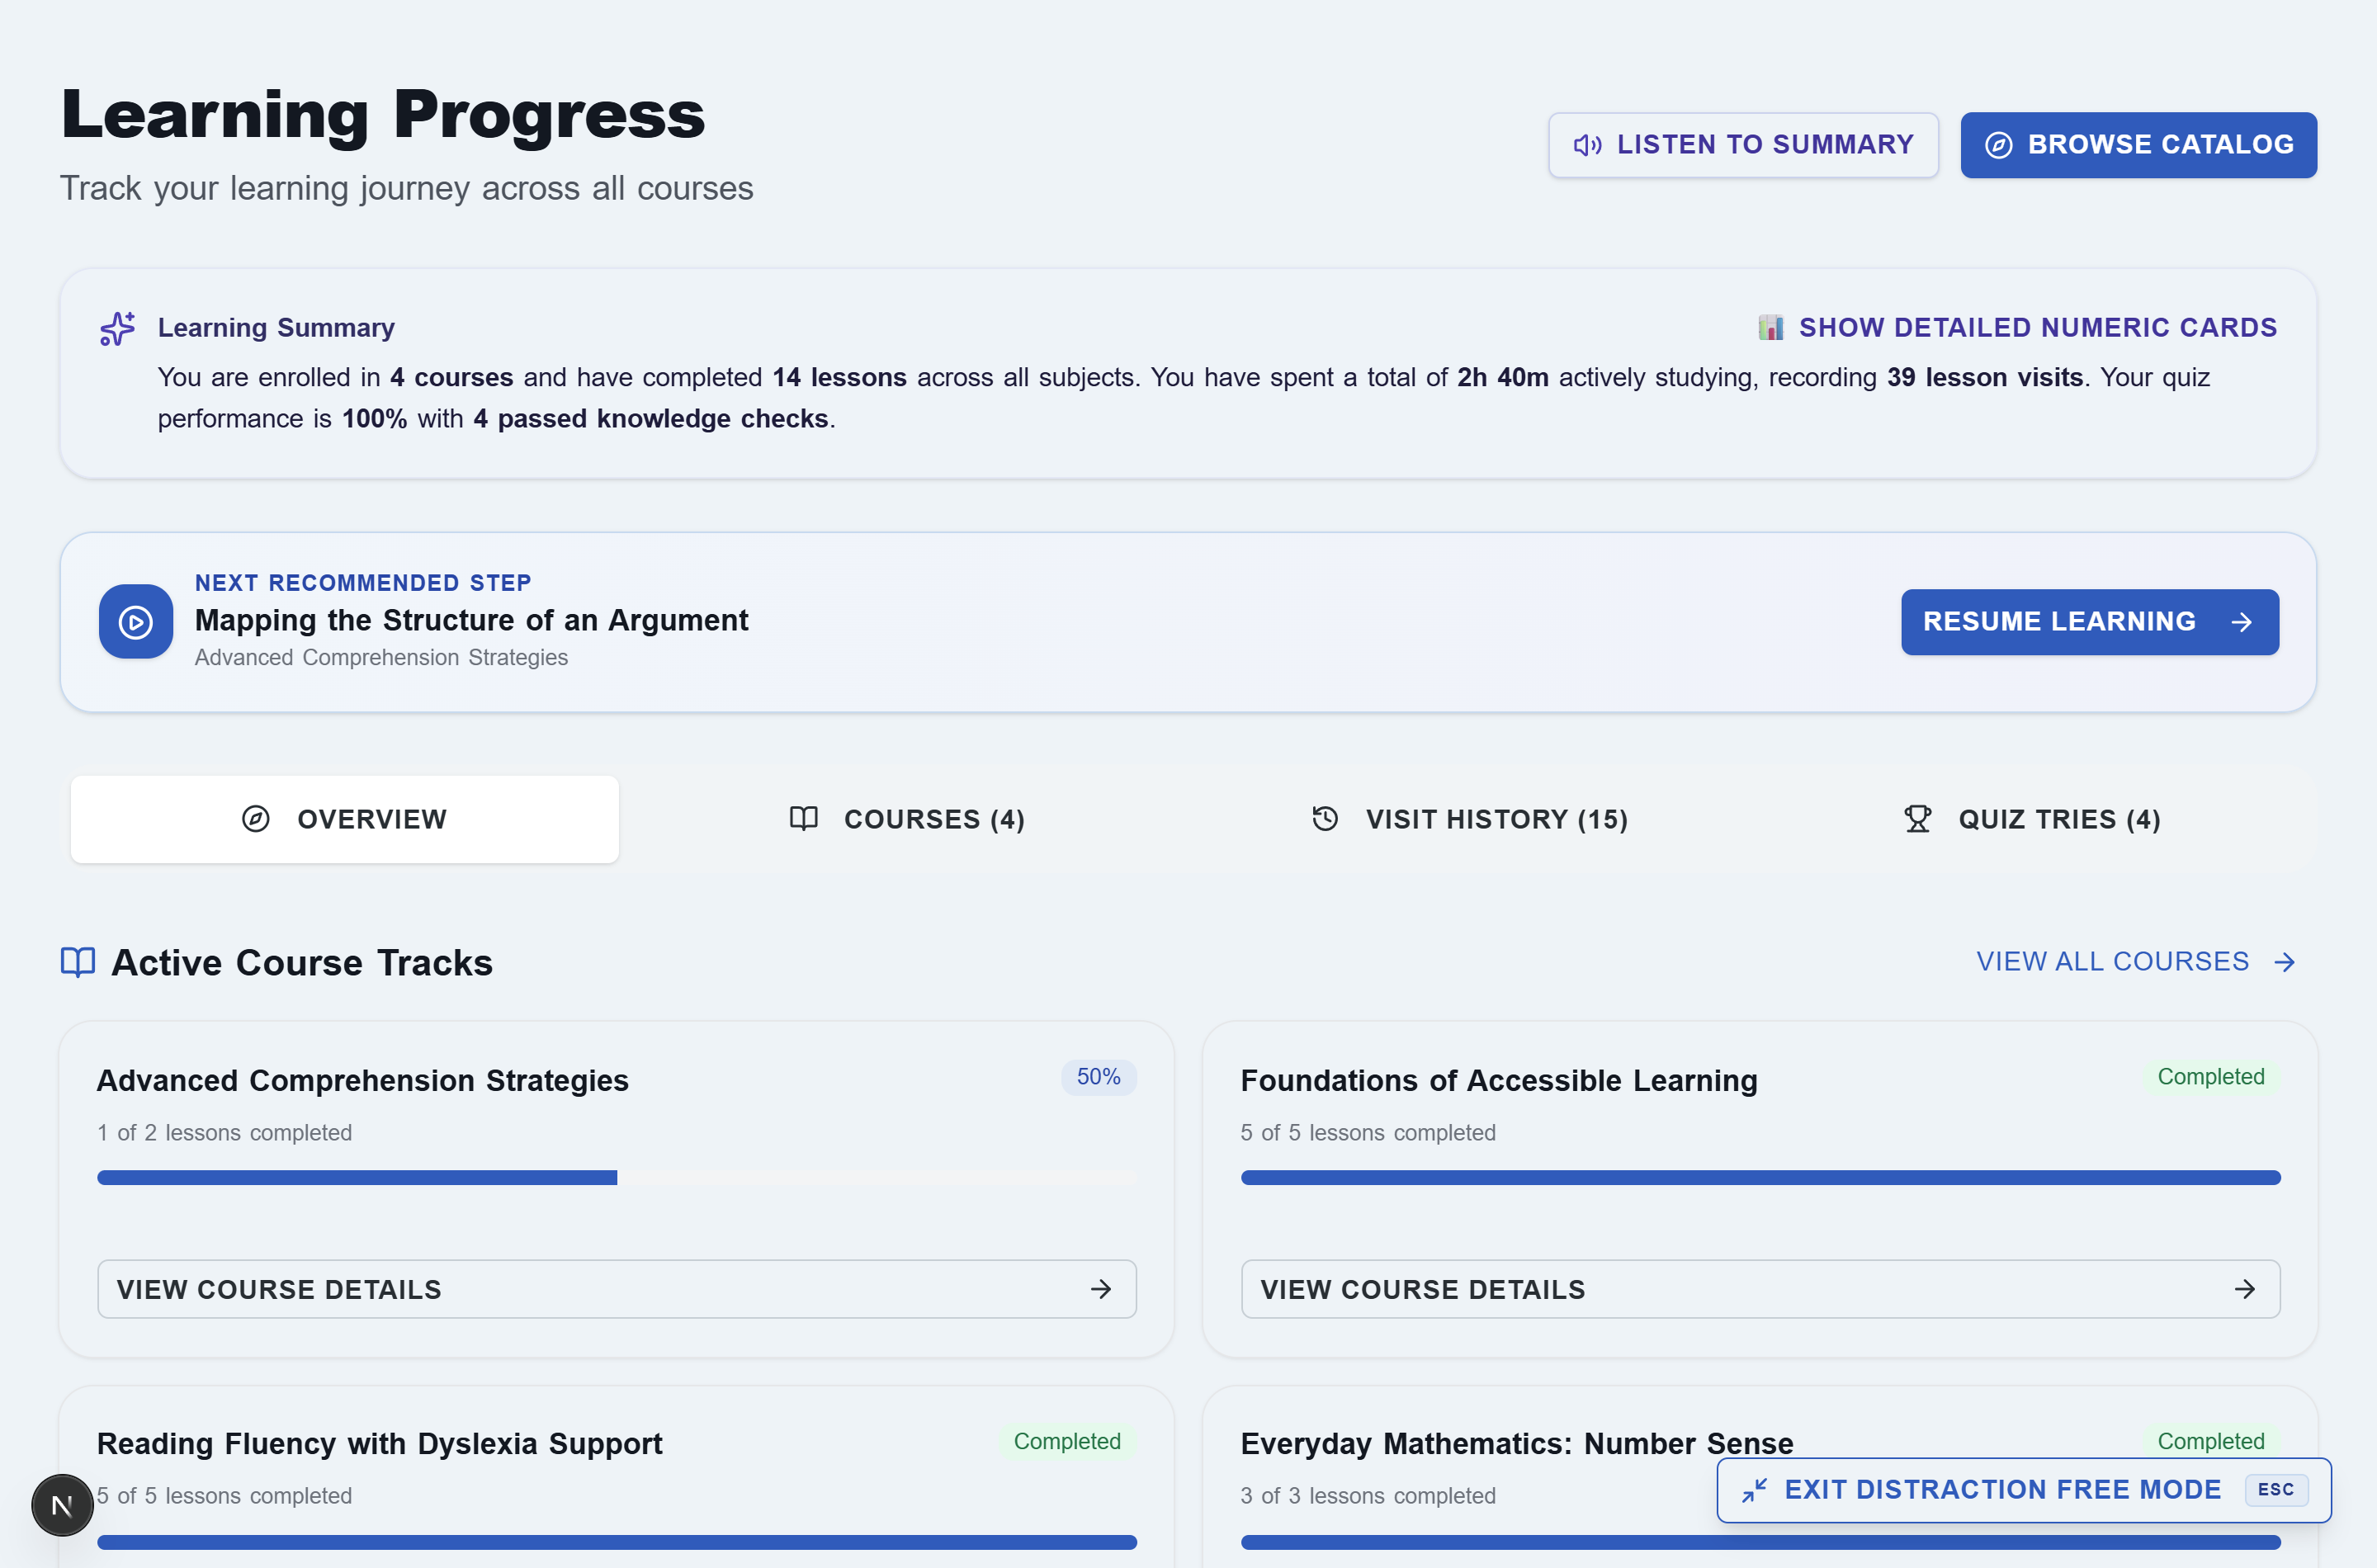
\includegraphics[width=0.92\textwidth]{Screenshots/learner-progress.png}
\caption{Learner Progress Page}
\label{fig:ui_learner_progress}
\end{figure}

\begin{figure}[htbp]
\centering
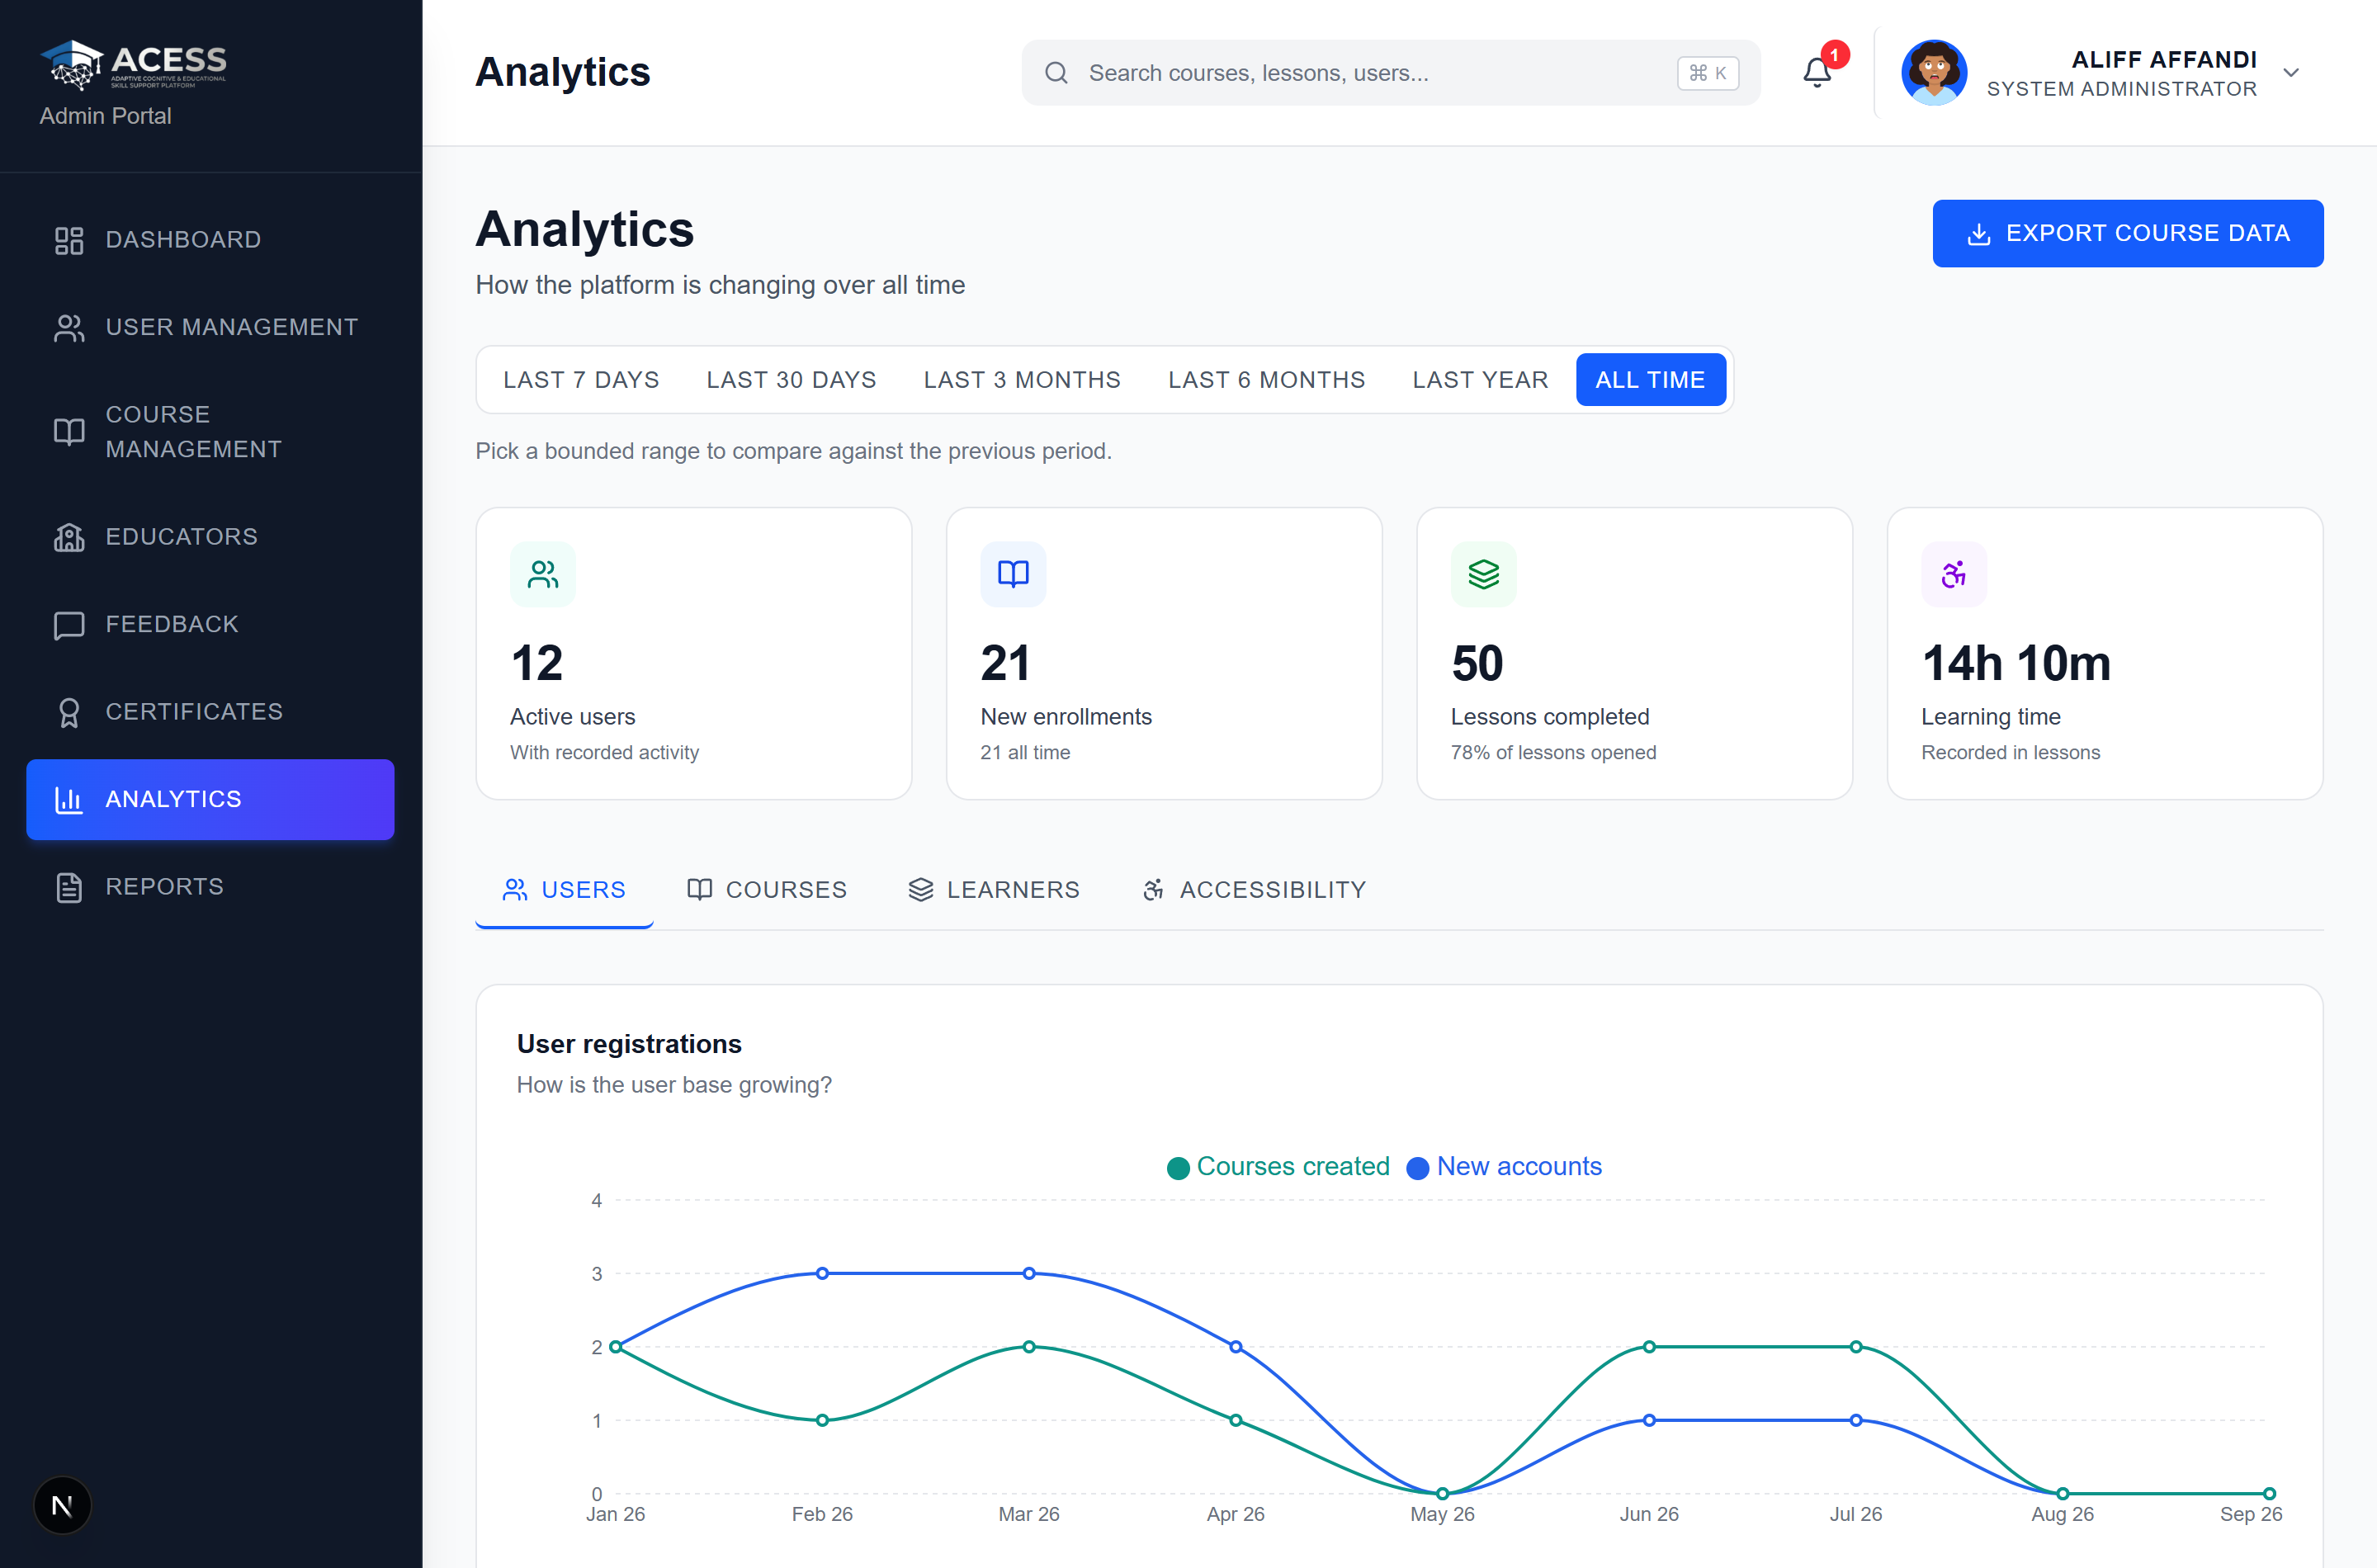
\includegraphics[width=0.92\textwidth]{Screenshots/admin-analytics.png}
\caption{Administrator Analytics Dashboard}
\label{fig:ui_admin_analytics}
\end{figure}

One output deserves separate mention because it is unusual in a learning platform. The administrator analytics view includes an Accessibility tab, shown in Figure~\ref{fig:ui_admin_a11y}, which reports which accessibility features are actually being used and which presets learners actually select. Accessibility features are often built and then never measured; this view exists so that the question of whether they are used has an answer.

\begin{figure}[htbp]
\centering
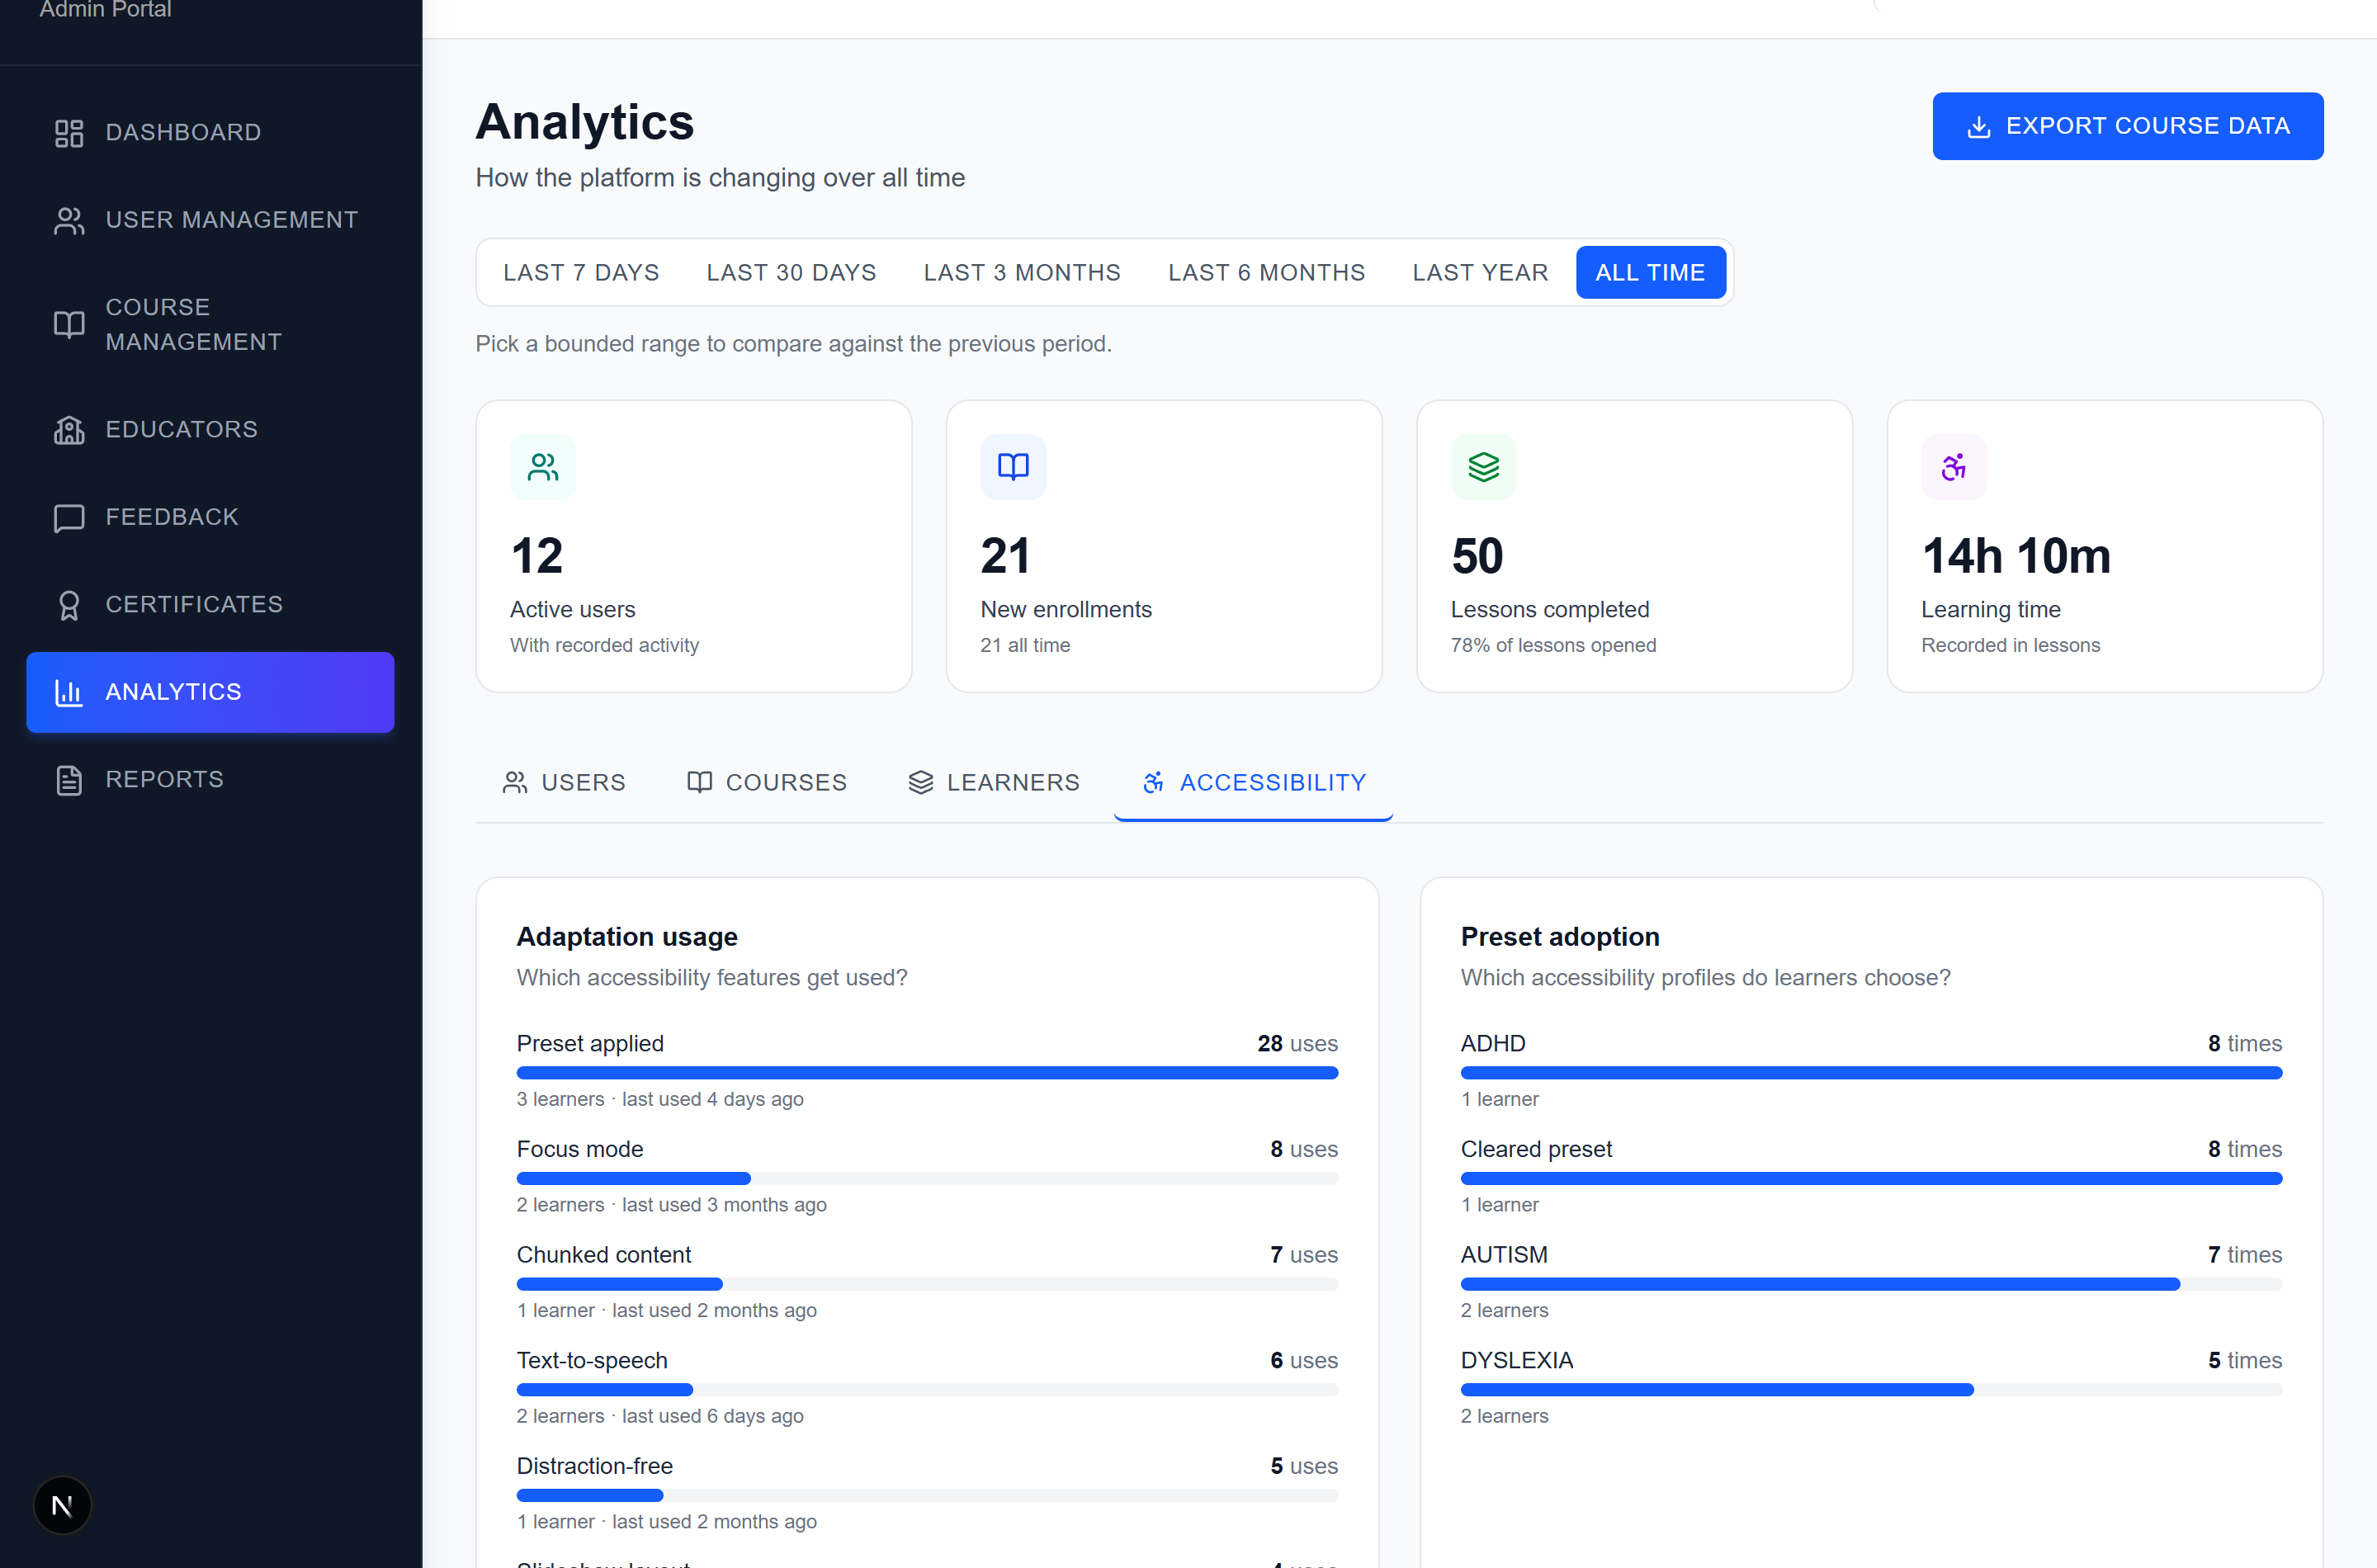
\includegraphics[width=0.92\textwidth]{Screenshots/admin-analytics-accessibility.png}
\caption{Accessibility Analytics}
\label{fig:ui_admin_a11y}
\end{figure}

\subsubsection{Conceptual and Logical Database Design}
\label{sec:erd}

The ACESS data model is a normalised relational schema implemented on PostgreSQL. It comprises 36 tables, one view, 370 columns, 57 foreign keys, 33 value constraints, 20 uniqueness constraints, 115 indexes, 20 functions, 15 triggers and 88 access policies. These figures were obtained by querying the system catalogue of a database rebuilt from the project's own schema definitions rather than estimated, and the same query can be re-run to confirm them.

The entity relationship diagrams in this section were generated from that live schema by a script in the project repository rather than drawn by hand, so that a diagram in this report cannot fall out of step with the database it describes. Because thirty-six entities cannot be shown legibly on a single portrait page, the model is presented as three domain diagrams followed by the complete schema in landscape orientation.

\paragraph{Business rules governing the relationships}

The following rules were derived from the operational requirements of the platform, and they are what the foreign keys, uniqueness rules and deletion rules in the schema encode.

\begin{enumerate}
    \item \textbf{One account has one profile.} Every account has exactly one extended profile, which is removed automatically when the account is removed.
    \item \textbf{A course must have an owner, and that owner cannot be removed.} Deleting the educator who owns a course is refused. This is the only such restriction in the schema, and it exists so that removing an account cannot silently destroy courses other people are enrolled in.
    \item \textbf{A learner enrols in a course at most once.} A uniqueness rule over the learner and course pair enforces this. Enrolling again reactivates the existing enrolment rather than creating a second one, which keeps the learner's progress history continuous.
    \item \textbf{All learning activity belongs to the enrolment.} Progress, quiz attempts, checkpoints, recommendations and certificates all reference the enrolment rather than the learner directly, so that the enrolment is the single unit of participation and withdrawing a learner from one course affects nothing else.
    \item \textbf{A lesson belongs to exactly one course and optionally to one chapter.} The course link is required; the chapter link is optional, because chapter organisation is a feature an educator may or may not use.
    \item \textbf{A lesson may declare one prerequisite lesson.} If that prerequisite is later removed, the requirement is cleared rather than leaving the dependent lesson unusable.
    \item \textbf{Assessment is strictly hierarchical.} A lesson has at most one quiz, a quiz has many questions, and a question has many answer options of which exactly one is correct. An attempt records one answer per question, and an option referenced by a submitted attempt cannot be deleted.
    \item \textbf{One certificate per enrolment.} A revoked certificate keeps its record and its reference code, with its status changed to revoked, and a constraint requires a revoked record to carry a revocation date while an issued one does not. This is what allows public verification to report that a certificate was revoked rather than that it does not exist.
    \item \textbf{An achievement is earned once per learner per course.} The record links the learner, the achievement definition and the course, and records are created only by the platform's own derivation logic.
    \item \textbf{Comments form a thread.} A comment may reference another comment as its parent, which gives one level of reply nesting.
    \item \textbf{Accessibility settings belong to the learner, not to an enrolment.} A learner's presentation preferences follow them across every course, so they are stored on the learner's profile.
\end{enumerate}

\paragraph{Domain 1: identity, access and platform}

Figure~\ref{fig:erd_identity} shows the identity domain. It holds the account record, the extended profile carrying accessibility and notification preferences, the educator application workflow, referral codes, notifications, reusable accessibility content templates, and the records of which accessibility features are actually used. Every entity in this domain references the account record directly, which is why its access policies are the simplest in the schema.

\begin{figure}[htbp]
\centering
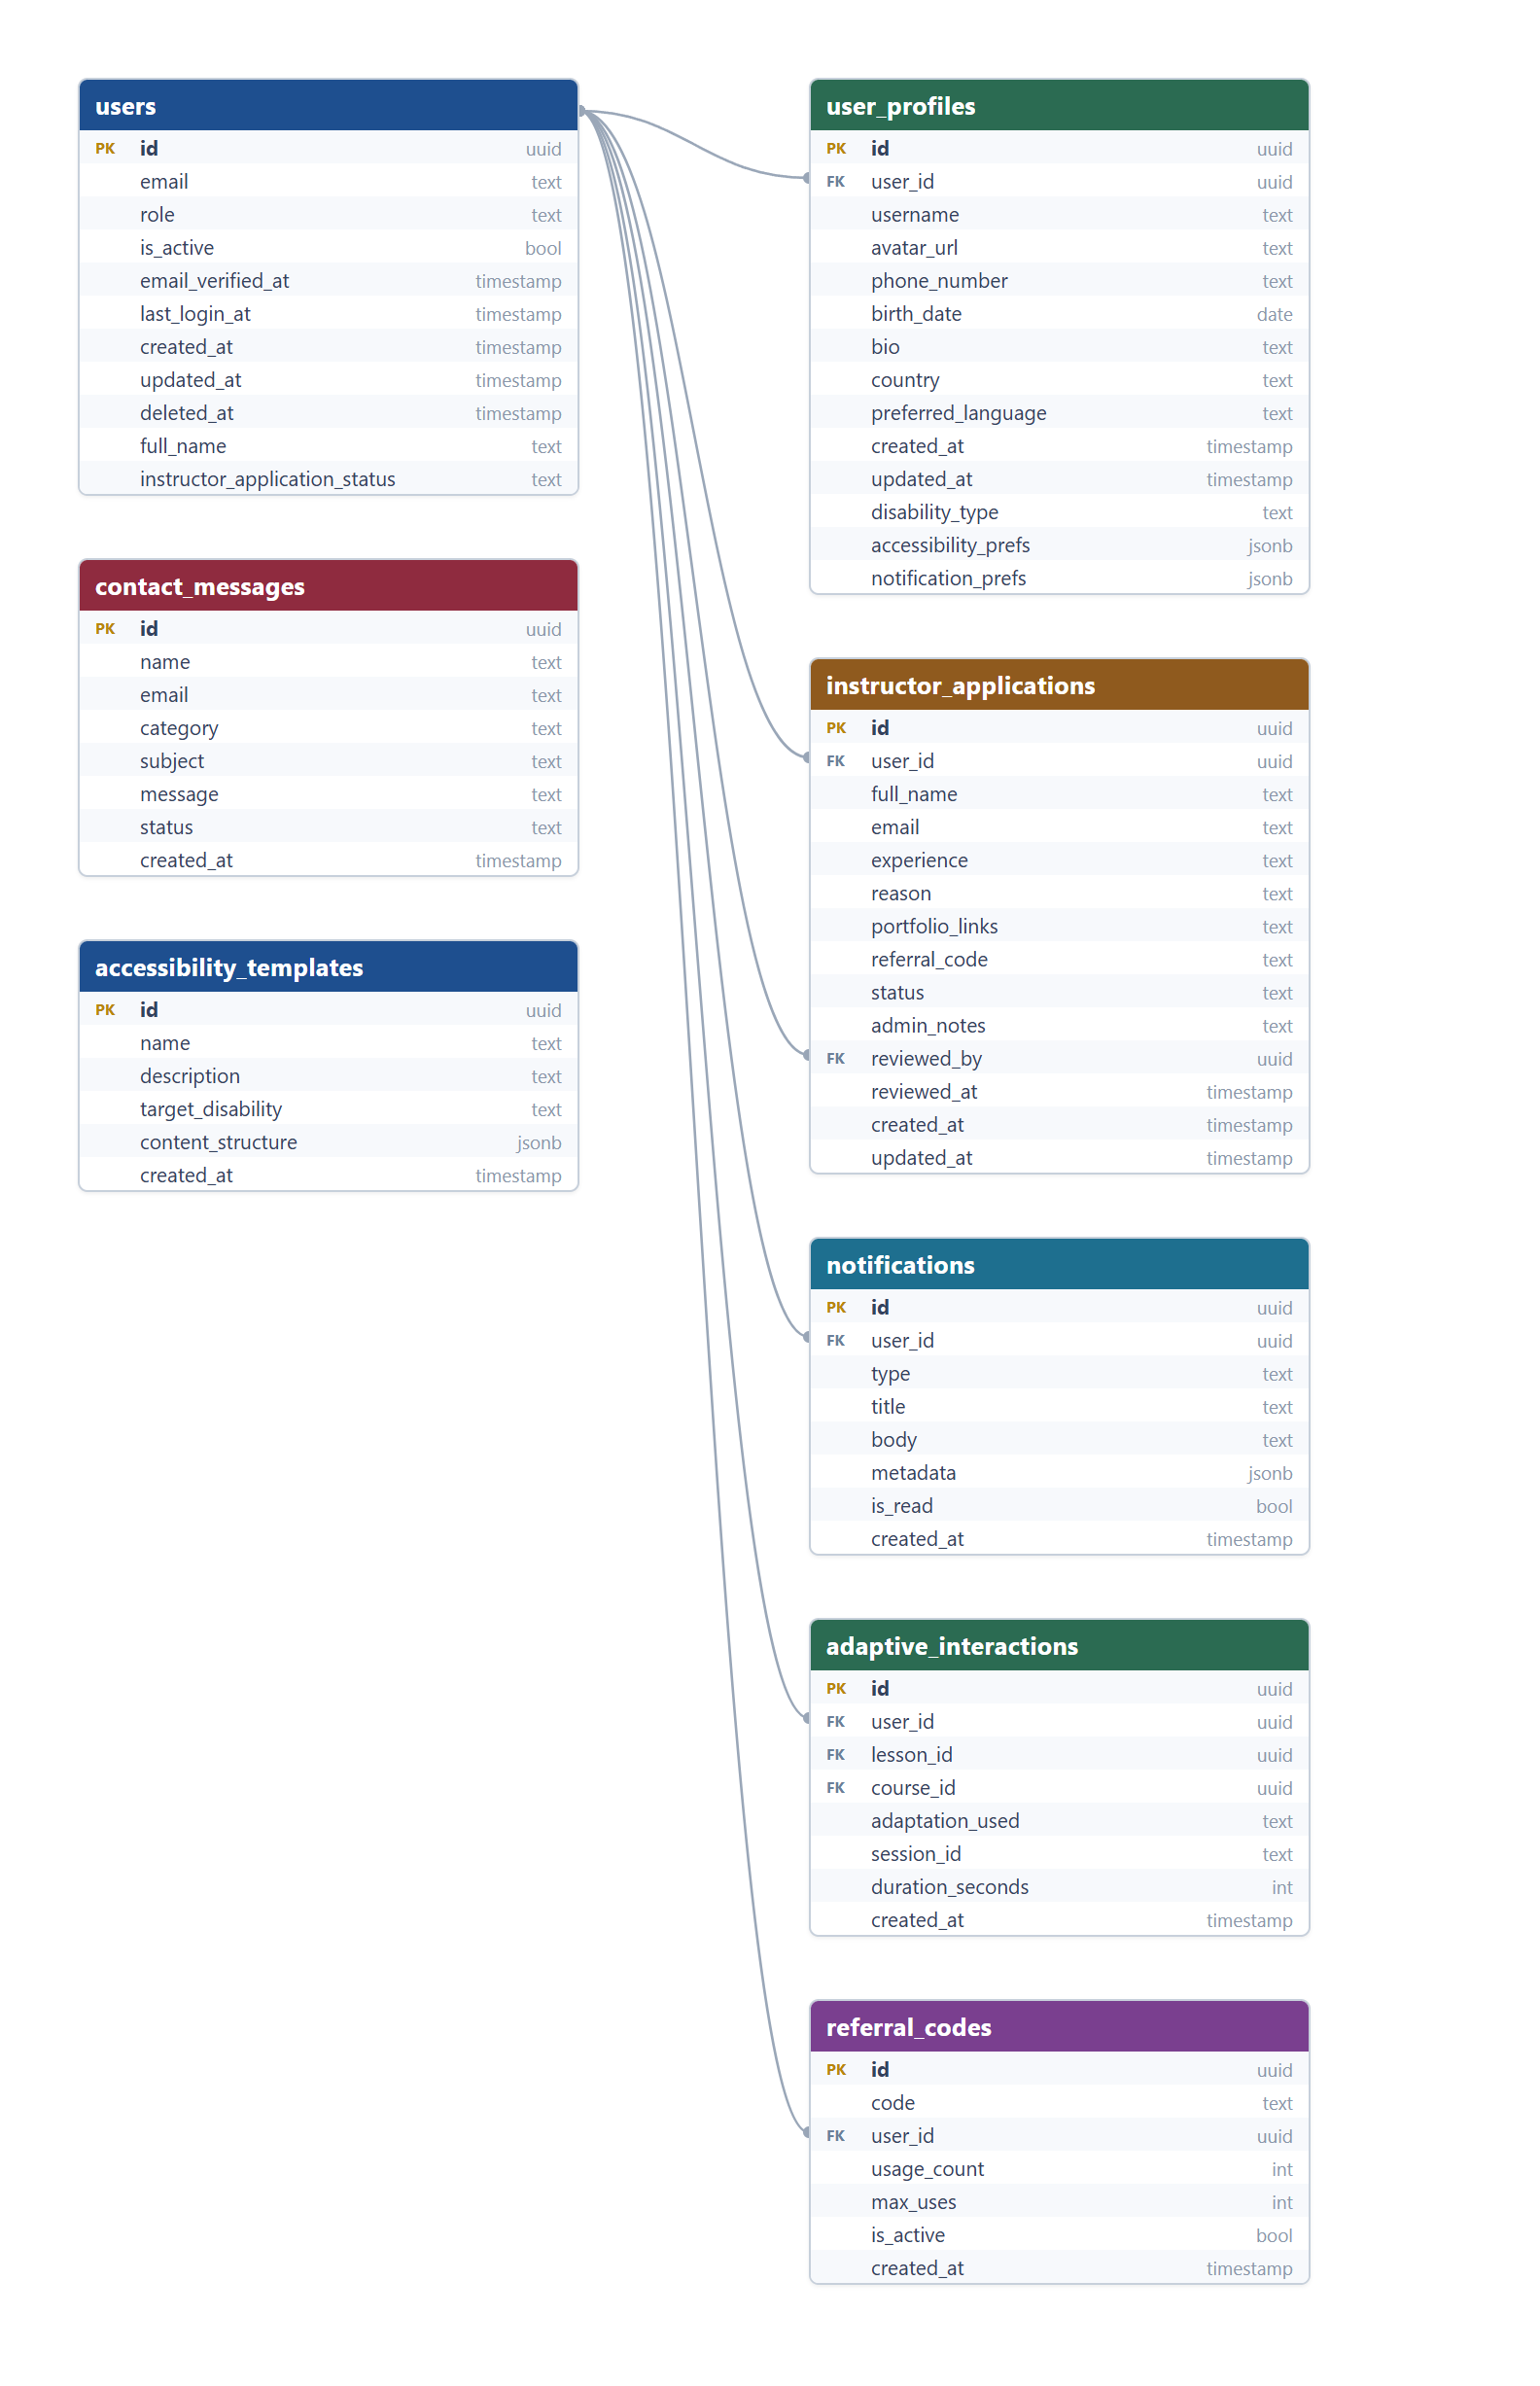
\includegraphics[width=\textwidth,height=0.84\textheight,keepaspectratio]{Diagram/ERD-1-identity.png}
\caption{Identity, Access and Platform Entity Relationship Diagram}
\label{fig:erd_identity}
\end{figure}

\paragraph{Domain 2: curriculum and content}

Figure~\ref{fig:erd_curriculum} shows the curriculum domain. It holds the course, chapter and lesson hierarchy, the artefacts attached to a lesson (interactive activities, in-video questions, embedded content, checkpoints, stored lesson summaries and discussion threads), and the supporting infrastructure of templates, version snapshots and uploaded media. Everything in this domain is authored by an educator.

\begin{figure}[htbp]
\centering
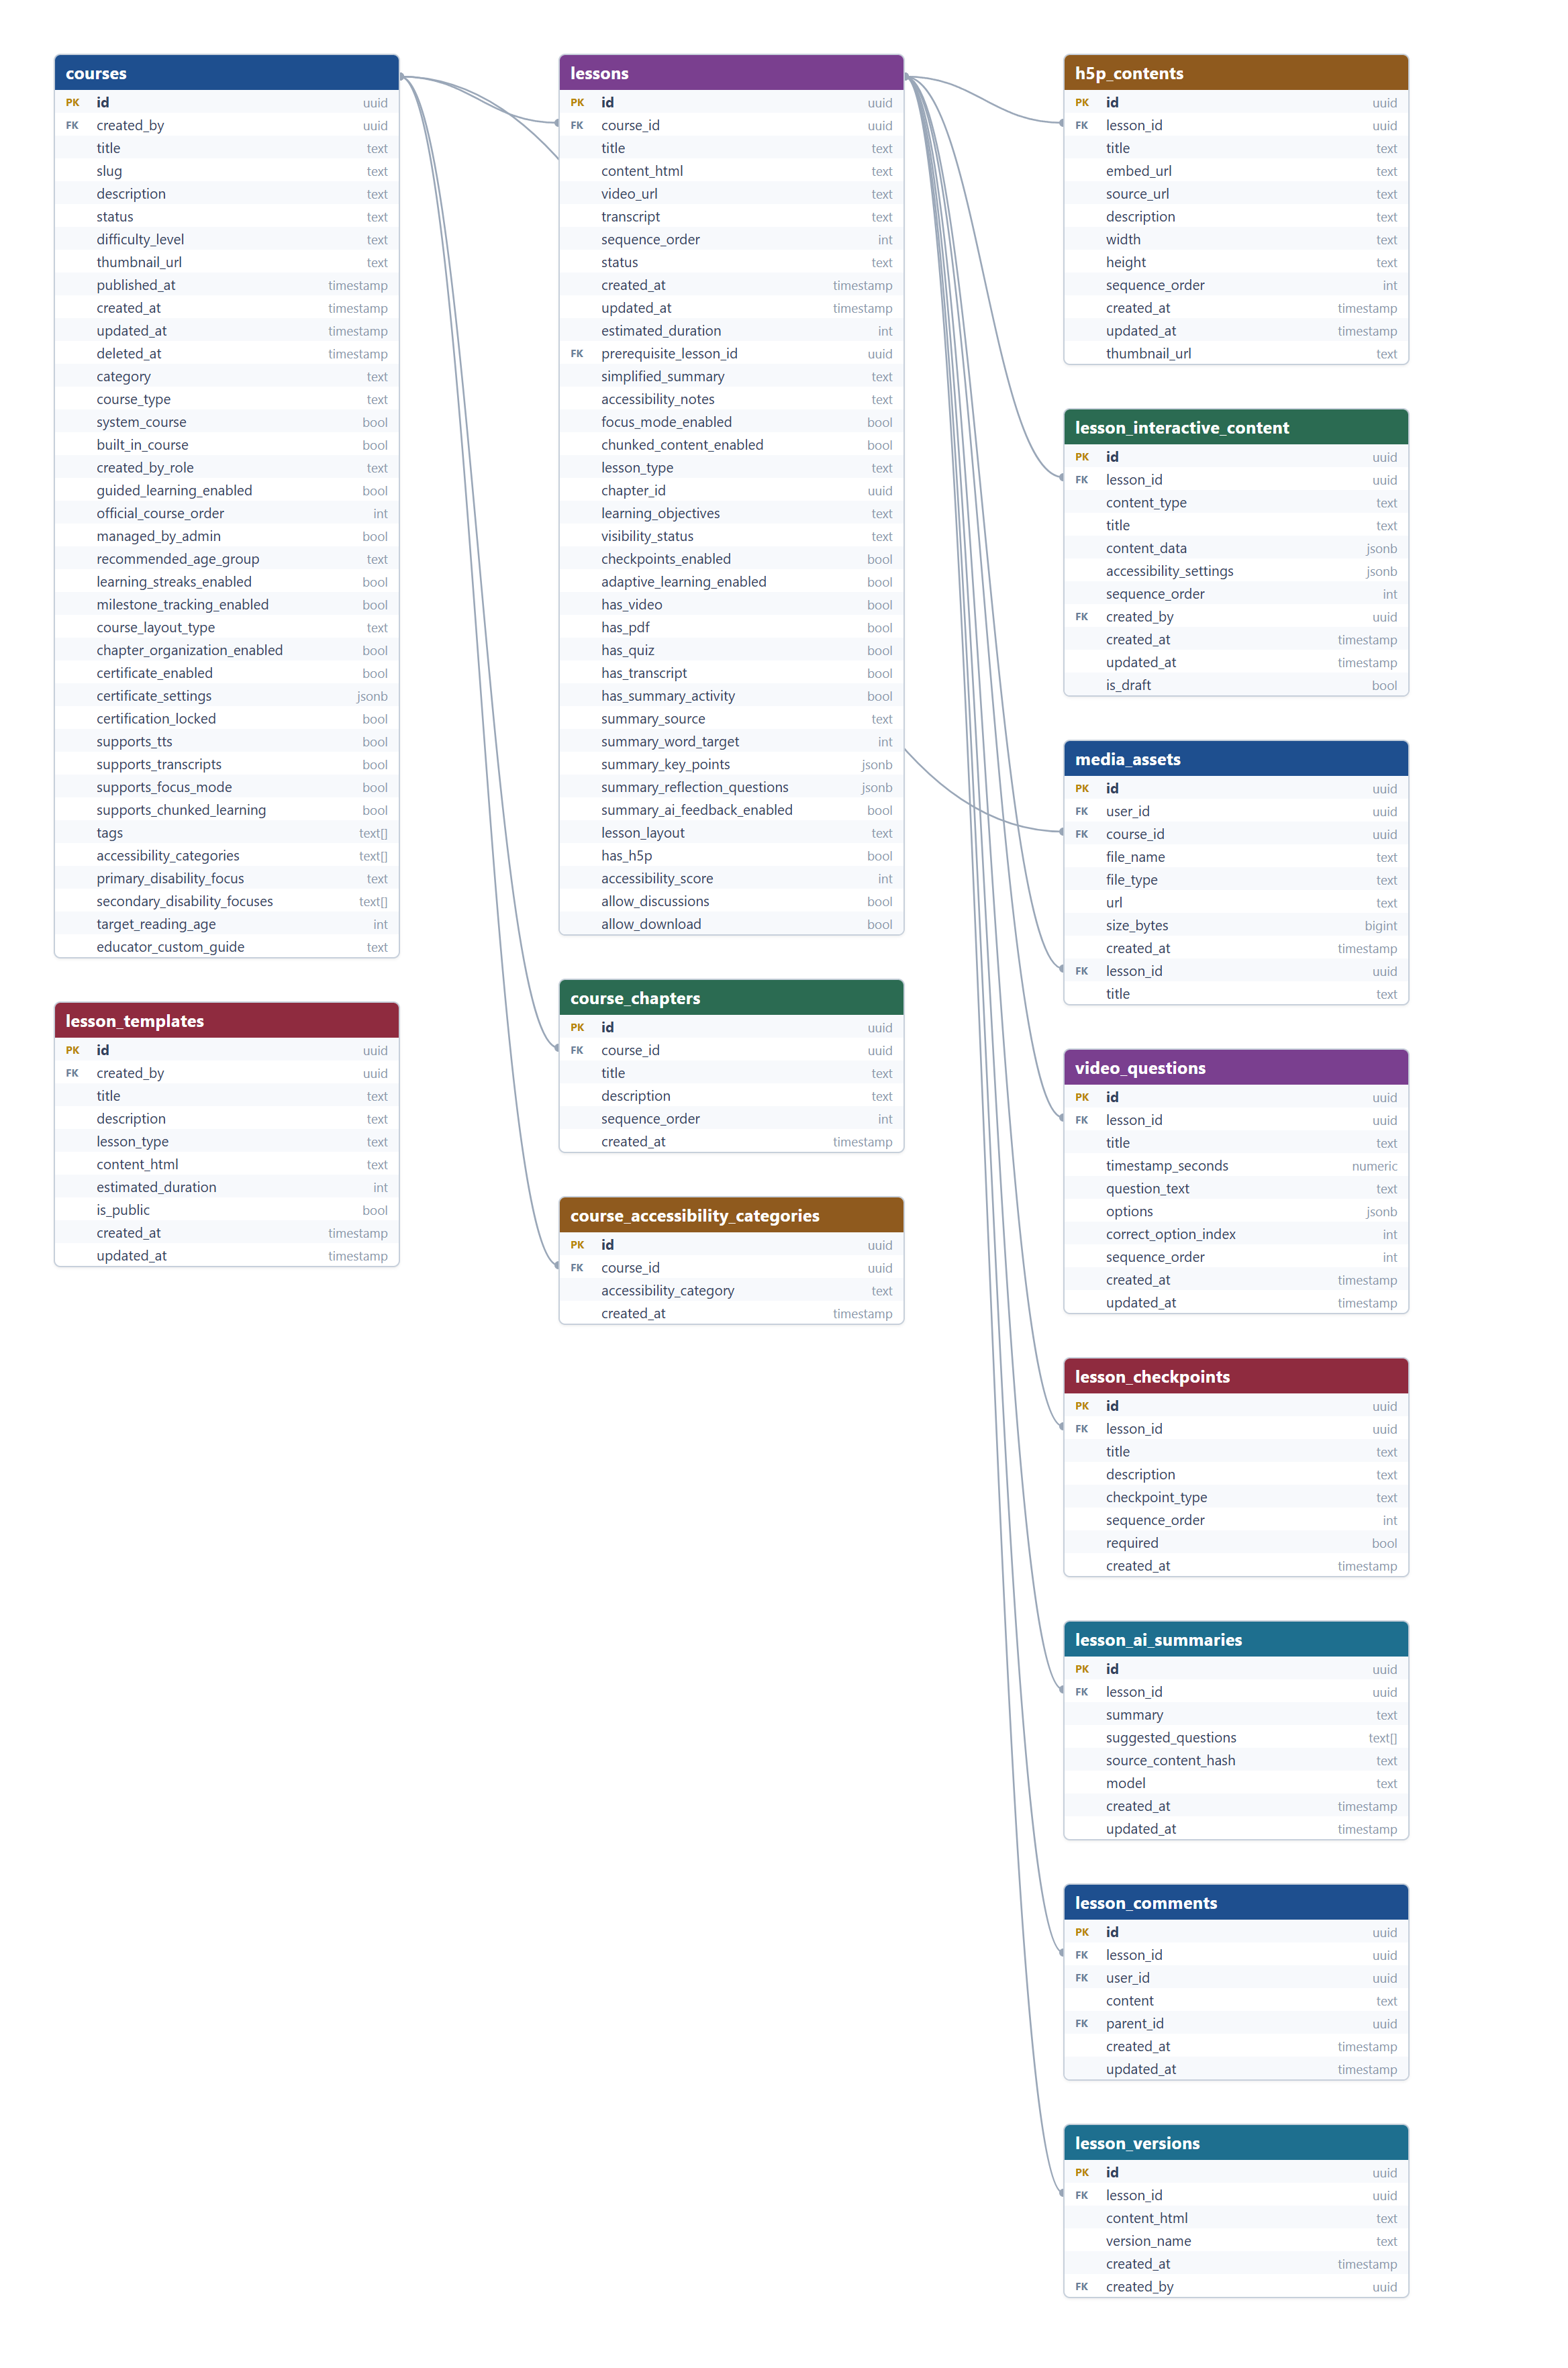
\includegraphics[width=\textwidth,height=0.84\textheight,keepaspectratio]{Diagram/ERD-2-curriculum.png}
\caption{Curriculum and Content Entity Relationship Diagram}
\label{fig:erd_curriculum}
\end{figure}

\paragraph{Domain 3: assessment, learning record and recognition}

Figure~\ref{fig:erd_assessment} shows the assessment and learning record domain, which holds everything generated by a learner: the enrolment itself, per-lesson progress, quiz attempts and answers, checkpoint and activity responses, generated recommendations, saved courses, and the recognition records of achievements, milestones and certificates. The convergence of these entities on the enrolment is what business rule~4 above describes.

\begin{figure}[htbp]
\centering
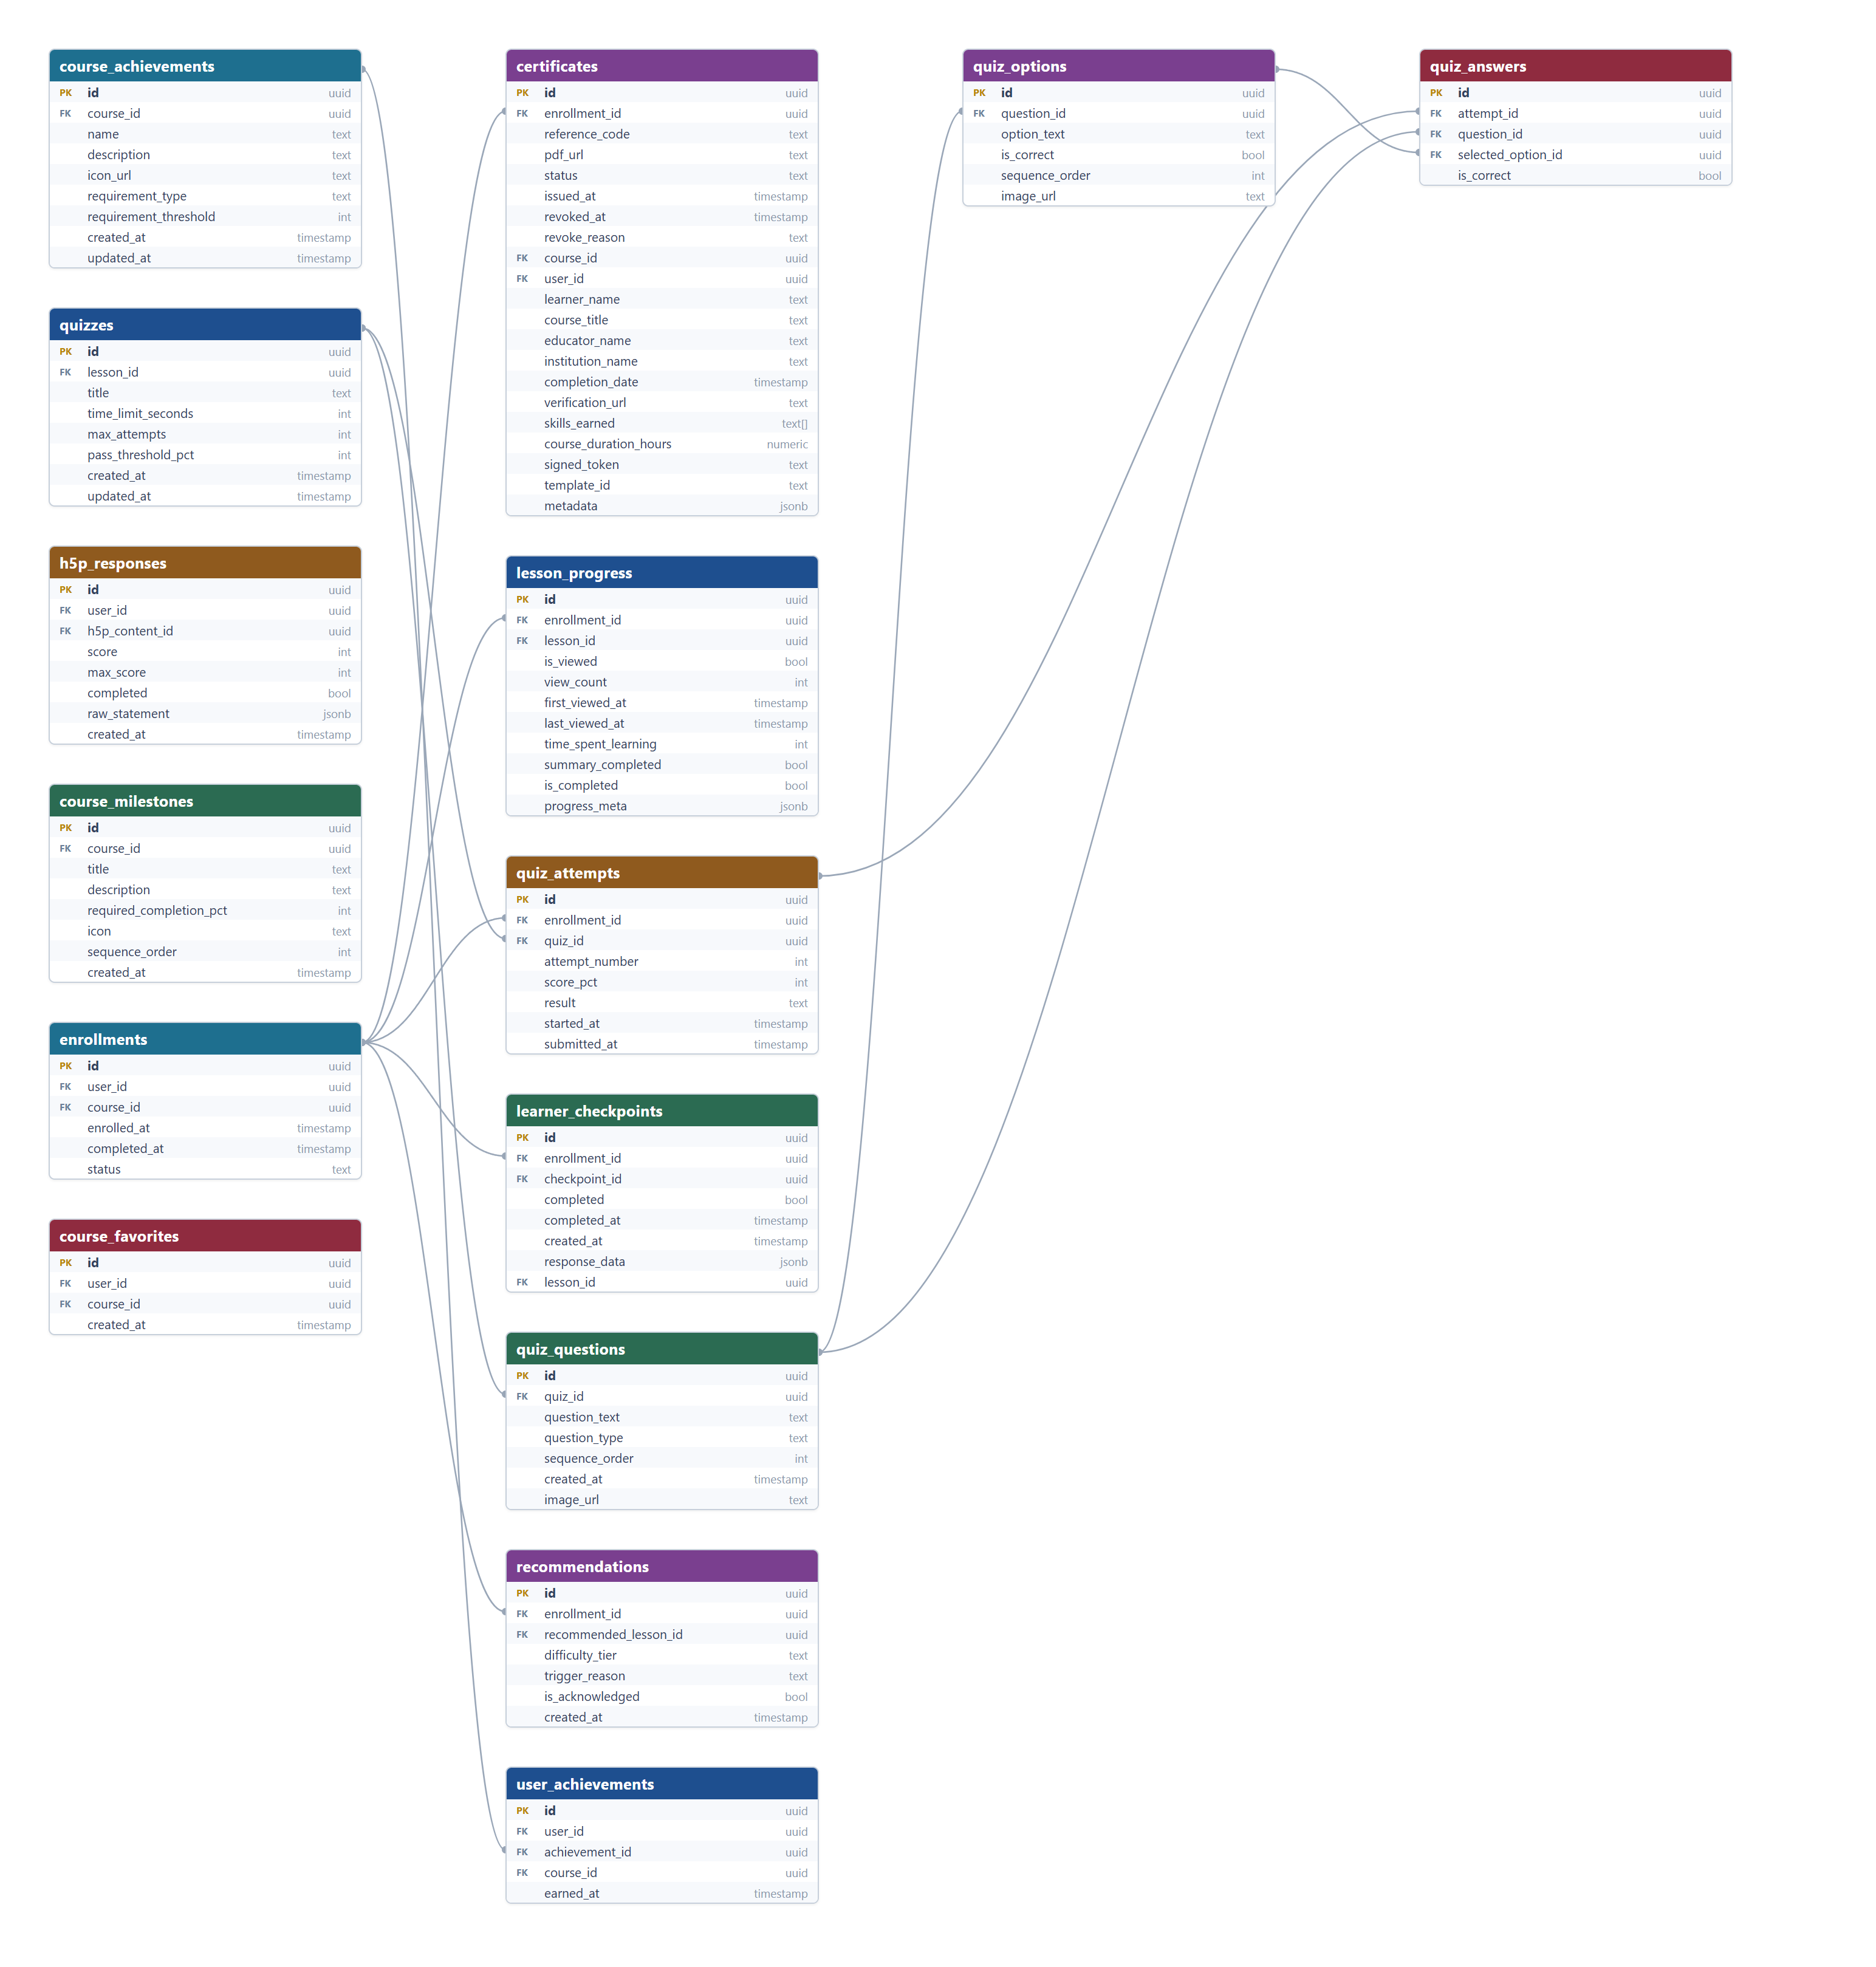
\includegraphics[width=\textwidth,height=0.84\textheight,keepaspectratio]{Diagram/ERD-3-assessment.png}
\caption{Assessment, Learning Record and Recognition Entity Relationship Diagram}
\label{fig:erd_assessment}
\end{figure}

\begin{landscape}
\begin{figure}[H]
\centering
% Explicit dimensions rather than \textwidth/\textheight: inside the rotated
% frame those two no longer correspond to the physical page edges.
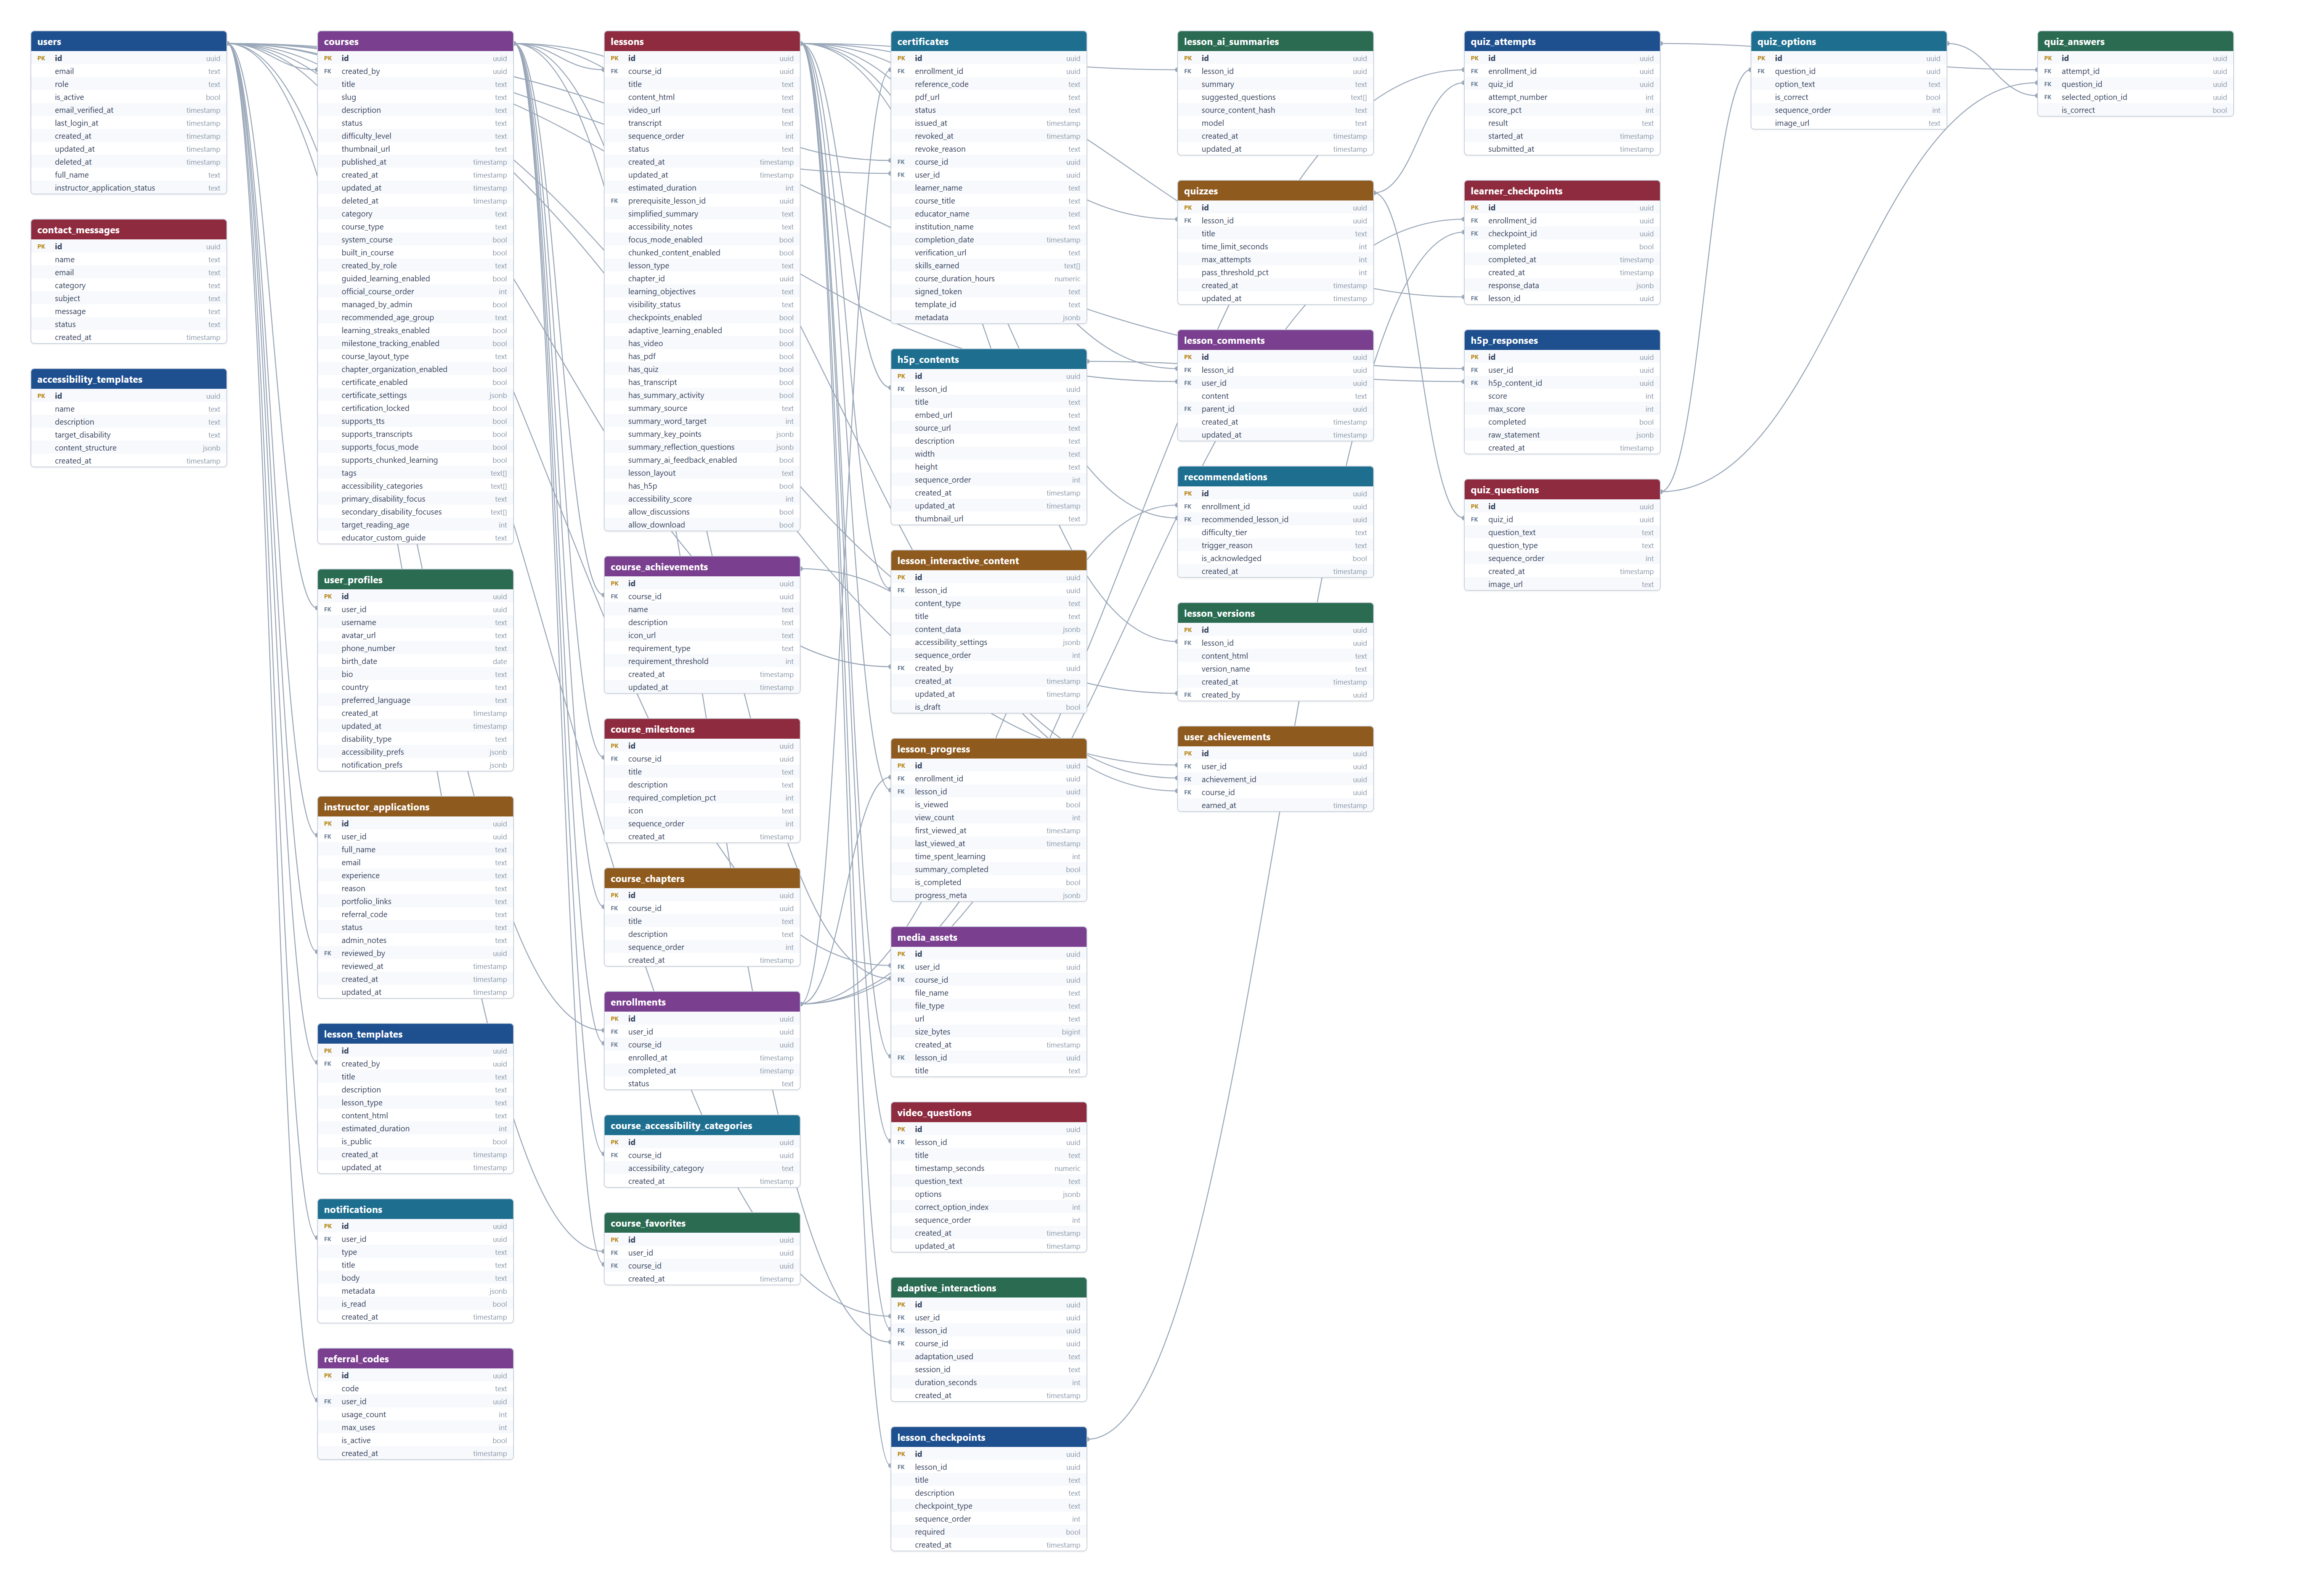
\includegraphics[width=20cm,height=13.3cm,keepaspectratio]{Diagram/ERD-0-overview.png}
\caption{Complete ACESS Entity Relationship Diagram}
\label{fig:erd}
\end{figure}
\end{landscape}

Figure~\ref{fig:erd} presents the full model of all 36 tables and 57 foreign keys. The account record acts as the identity hub and the enrolment as the participation hub: nearly every record generated by a learner reaches the account record through an enrolment rather than directly, which is what allows most access policies to be expressed as a single relationship check.

\subsection{Accessibility Design}
\label{sec:a11y-design}

\subsubsection{Design approach and standards baseline}

Accessibility in ACESS is treated as a design constraint that the rest of the system is arranged around rather than as a settings panel added to a finished product. Three commitments follow from that position, and they explain most of the design decisions in this section.

The first is that a control must do what its label says. During development several settings were found to have no effect: a word-spacing control that a stylesheet rule silently overrode, a line-spacing control that changed the settings preview but not the lesson itself, and a simplified reading mode that could not be reached from anywhere in the interface. Each of these appeared to work and did not. They were corrected, and the platform now maintains an explicit catalogue of every learner-facing setting, checked automatically, under the rule that a setting which is not in the catalogue does not exist. Two settings that still do not fully match their labels are recorded as known gaps in Section~\ref{sec:a11y-gaps} rather than presented as working.

The second is that the standards baseline has to be wider than WCAG. WCAG~2.2 is necessary but was not written primarily for cognitive difference: it can establish that contrast is insufficient, but not that a paragraph is too long for a learner to re-enter after being interrupted. ACESS therefore works from three sources together: WCAG~2.2 \cite{wcag22} for testable technical criteria, the W3C guidance on making content usable for people with cognitive and learning disabilities \cite{wcag_cognitive} for cognitive design objectives, and the British Dyslexia Association Style Guide \cite{bda_style_guide} for typographic and readability thresholds.

The third is that the claim must not exceed the evidence. ACESS targets WCAG~2.2 Level~AA together with four Level~AAA criteria. It has not been independently audited, has not been tested with a screen reader or other assistive technology, and has not been tested with neurodivergent learners. That statement is published on the platform's own accessibility statement page, where a prospective learner can read it, and it is repeated in Section~\ref{sec:a11y-gaps}.

\subsubsection{Mapping of standards to implementation}

Table~\ref{tab:wcag_map} maps each addressed criterion to the ACESS feature that addresses it, the learner profile it primarily serves, and the part of the system in which it is implemented. The final column names the figure in this report that shows it, where one exists.

{
\renewcommand{\arraystretch}{1.15}
\setstretch{1.05}
\scriptsize
\begin{longtable}{|>{\raggedright\arraybackslash\tabbreak}p{2.0cm}|>{\raggedright\arraybackslash\tabbreak}p{4.0cm}|>{\raggedright\arraybackslash\tabbreak}p{1.3cm}|>{\raggedright\arraybackslash\tabbreak}p{3.2cm}|>{\raggedright\arraybackslash\tabbreak}p{1.75cm}|}
\caption{Mapping of Accessibility Criteria to ACESS Features}
\label{tab:wcag_map}\\
\hline
\textbf{Criterion} & \textbf{ACESS feature addressing it} & \textbf{Profile served} & \textbf{Implemented in} & \textbf{Evidence} \\
\hline \hline
\endfirsthead
\multicolumn{5}{l}{\footnotesize\itshape Table~\ref{tab:wcag_map} continued from the previous page}\\
\hline
\textbf{Criterion} & \textbf{ACESS feature addressing it} & \textbf{Profile served} & \textbf{Implemented in} & \textbf{Evidence} \\
\hline \hline
\endhead
\hline
\multicolumn{5}{r}{\footnotesize\itshape continued on the next page}\\
\endfoot
\endlastfoot
1.1.1 Non-text Content (A) & The compliance checker requires alternative text on every image and provides a field to supply it & All & Compliance checker & Fig.~\ref{fig:ui_edu_a11y} \\ \hline
1.2.1 Video-only (A) & A lesson containing video but no transcript is reported as a required failure & All & Compliance checker, lesson record & Fig.~\ref{fig:ui_edu_a11y} \\ \hline
1.2.2 Captions (A) & Captions are shown on video by default when the learner enables the setting & Hearing, slower processing & Accessibility module & Fig.~\ref{fig:ui_a11y_modal} \\ \hline
1.3.1 Info and Relationships (A) & The checker rejects empty paragraphs used as spacing and requires real headings & All & Compliance checker & Fig.~\ref{fig:ui_edu_a11y} \\ \hline
1.4.4 Resize Text (AA) & Text size adjustable between 12 and 24\,px, applied without reloading the page & Dyslexia & Accessibility module & Fig.~\ref{fig:ui_a11y_modal} \\ \hline
1.4.5 Images of Text (AA) & The checker requires body content to be real text so that read-aloud can reach it & Dyslexia & Compliance checker & Fig.~\ref{fig:ui_edu_a11y} \\ \hline
1.4.8 Visual Presentation (AAA) & Reading width bounded in character units (72 default, 62 Dyslexia, 66 ADHD) and retained when navigation is hidden & Dyslexia, ADHD & Stylesheet & Fig.~\ref{fig:preset_dyslexia} \\ \hline
1.4.12 Text Spacing (AA) & Line spacing between 1.0 and 3.0 and word spacing up to 0.2\,em, both learner-set, with the Dyslexia preset at the required 0.16\,em & Dyslexia & Accessibility module & Fig.~\ref{fig:preset_dyslexia} \\ \hline
2.2.1 Timing Adjustable (A) & A quiz time limit set by an educator is displayed to the learner & ADHD, Autism & Quiz interface & Fig.~\ref{fig:ui_quiz} \\ \hline
2.2.4 Interruptions (AAA) & Distraction-free mode removes navigation and notification elements during a lesson & ADHD & Stylesheet, lesson view & Fig.~\ref{fig:preset_adhd} \\ \hline
2.2.6 Timeouts (AAA) & A fifteen-minute inactivity timeout announced by a warning thirty seconds beforehand & All & Session timeout component & N/A \\ \hline
2.3.3 Animation (AAA) & One motion control (normal, low or none) reduces or removes animation across the site & Autism, ADHD & Accessibility module & Fig.~\ref{fig:ui_a11y_modal} \\ \hline
2.4.4 Link Purpose (A) & The checker flags link text that does not describe its destination & All & Compliance checker & Fig.~\ref{fig:ui_edu_a11y} \\ \hline
2.4.6 Headings and Labels (AA) & The checker requires headings once a lesson passes 200 words & All & Compliance checker & Fig.~\ref{fig:ui_edu_a11y} \\ \hline
3.1.5 Reading Level (AAA) & The checker computes a Flesch--Kincaid grade level and compares it with the course's target reading age \cite{kincaid1975derivation} & Dyslexia & Compliance checker & Fig.~\ref{fig:ui_edu_a11y} \\ \hline
3.2.3 Consistent Navigation (AA) & Identical shell and navigation order on every page of a role, and the checker verifies structural consistency between lessons of one course & Autism & Navigation, compliance checker & Fig.~\ref{fig:ui_learner_dashboard} \\ \hline
3.2.5 Change on Request (AAA) & A preset shows exactly what it will change before applying it, read-aloud never starts by itself, and no media plays automatically & All & Preset preview dialog & Fig.~\ref{fig:preset_diff} \\ \hline
4.1.2 Name, Role, Value (A) & Navigation built from real links carrying current-page state, and icon-only controls given accessible names and states & All & Navigation and lesson header & Fig.~\ref{fig:ui_learner_dashboard} \\ \hline
W3C cognitive guidance, objectives 3--5 & Content presented in sections, per-section time estimates, visual schedule and step-by-step guidance & ADHD, Autism & Visual schedule and guidance components & Fig.~\ref{fig:preset_autism} \\ \hline
\end{longtable}
}

Table~\ref{tab:wcag_map} makes one structural point worth drawing out. The criteria divide into two groups according to who can satisfy them. Presentation criteria such as 1.4.4, 1.4.8, 1.4.12, 2.3.3, 2.2.6 and 3.2.5 are satisfied by the platform once, for every learner. Content criteria such as 1.1.1, 1.2.1, 1.3.1, 2.4.4, 2.4.6 and 3.1.5 cannot be satisfied by the platform at all, because they are properties of what an educator writes. A platform can only make the requirement visible at the moment of writing, which is what the accessibility compliance checker described in Section~\ref{sec:a11y-audit} exists to do.

\subsubsection{The three learner profiles}

Table~\ref{tab:profiles} states, for each of the three profiles the platform is designed around, the accessibility needs it addresses and the support ACESS provides. Every entry in the third column corresponds to a feature that is implemented.

{
\renewcommand{\arraystretch}{1.15}
\setstretch{1.05}
\scriptsize
\begin{longtable}{|>{\raggedright\arraybackslash\tabbreak}p{1.51cm}|>{\raggedright\arraybackslash\tabbreak}p{5.0cm}|>{\raggedright\arraybackslash\tabbreak}p{6.99cm}|}
\caption{Learner Profiles and the Support Provided by ACESS}
\label{tab:profiles}\\
\hline
\textbf{Profile} & \textbf{Main accessibility needs} & \textbf{ACESS support} \\
\hline \hline
\endfirsthead
\multicolumn{3}{l}{\footnotesize\itshape Table~\ref{tab:profiles} continued from the previous page}\\
\hline
\textbf{Profile} & \textbf{Main accessibility needs} & \textbf{ACESS support} \\
\hline \hline
\endhead
\hline
\multicolumn{3}{r}{\footnotesize\itshape continued on the next page}\\
\endfoot
\endlastfoot
Dyslexia &
\begin{tabular}[t]{@{}p{4.7cm}@{}}
\textbullet\ Reduced decoding effort \\
\textbullet\ Reduced visual crowding between letters, words and lines \\
\textbullet\ A reliable way to keep one's place in a long passage \\
\textbullet\ An alternative to reading \\
\textbullet\ Reduced glare over long sessions
\end{tabular} &
\begin{tabular}[t]{@{}p{6.7cm}@{}}
\textbullet\ Atkinson Hyperlegible or OpenDyslexic typeface, 19\,px base size, 1.7 line spacing \\
\textbullet\ Word spacing at the 0.16\,em value required by WCAG \\
\textbullet\ Reading width narrowed to 62 characters, within the 50 to 70 range recommended by the BDA \\
\textbullet\ Cream background, and a reading spotlight that dims all but the current paragraph \\
\textbullet\ Read-aloud with adjustable rate and a click-to-read-from-here control \\
\textbullet\ A reading toolbar carrying size, spacing, tint and spotlight controls without leaving the lesson \\
\textbullet\ Italic text rendered as bold, and text never justified \\
\textbullet\ Content presented one section at a time, on a single-column dashboard \\
\textbullet\ The compliance checker verifies sentence length and readability against the course's target reading age
\end{tabular} \\ \hline
ADHD &
\begin{tabular}[t]{@{}p{4.7cm}@{}}
\textbullet\ Sustained attention is costly \\
\textbullet\ Starting a task is difficult \\
\textbullet\ An interruption destroys one's place \\
\textbullet\ Passive reading is poorly retained \\
\textbullet\ Competing on-screen elements all draw attention equally
\end{tabular} &
\begin{tabular}[t]{@{}p{6.7cm}@{}}
\textbullet\ Distraction-free mode hiding the sidebar and notification area \\
\textbullet\ Reading width held at 66 characters, including while navigation is hidden \\
\textbullet\ A persistent bar carrying the current task and its progress \\
\textbullet\ A task checklist and a progress timeline \\
\textbullet\ An auto-save indicator, so that leaving the page carries no risk \\
\textbullet\ Reading spotlight \\
\textbullet\ Content divided into sections with a reading-time estimate for each \\
\textbullet\ The compliance checker caps a lesson at 20 minutes and an unbroken block at 150 words, expects a section break roughly every 400 words, expects video under six minutes or in-video questions, and requires at least one activity in every lesson
\end{tabular} \\ \hline
Autism &
\begin{tabular}[t]{@{}p{4.7cm}@{}}
\textbullet\ Uncertainty about what is coming is itself a barrier \\
\textbullet\ Sensory input can overload \\
\textbullet\ Figurative language must be decoded before the content can be \\
\textbullet\ Inconsistent structure has to be relearned each time
\end{tabular} &
\begin{tabular}[t]{@{}p{6.7cm}@{}}
\textbullet\ A visual schedule listing every phase of the lesson, with progress, before the learner starts \\
\textbullet\ Step-by-step guidance that states why a control is unavailable rather than only disabling it \\
\textbullet\ Checklist structure mode, which states expectations before each task \\
\textbullet\ Motion removed, colour saturation reduced, pale blue background \\
\textbullet\ Reading width fixed at the same value for every course, so pages do not change shape between lessons \\
\textbullet\ No automatic playback anywhere \\
\textbullet\ The compliance checker looks for figurative language, requires at least two stated learning objectives and a plain-language summary, and verifies structural consistency with the other lessons of the same course
\end{tabular} \\ \hline
\end{longtable}
}

\subsubsection{Preset composition}
\label{sec:preset-values}

An accessibility preset is not simply a theme. It is a single decision by the learner that sets nineteen individual values at once, covering typography, colour, layout, pacing and executive-function support. Table~\ref{tab:preset_effects} gives the exact values, taken from the platform's own preset definitions. Every one of these settings remains individually adjustable afterwards, so choosing a preset is a starting point rather than a mode the learner is locked into.

{
\renewcommand{\arraystretch}{1.18}
\setstretch{1.05}
\scriptsize
\begin{longtable}{|>{\raggedright\arraybackslash\tabbreak}p{3.08cm}|>{\raggedright\arraybackslash\tabbreak}p{2.24cm}|>{\raggedright\arraybackslash\tabbreak}p{2.24cm}|>{\raggedright\arraybackslash\tabbreak}p{2.24cm}|>{\raggedright\arraybackslash\tabbreak}p{2.24cm}|}
\caption{Accessibility Preset Values}
\label{tab:preset_effects}\\
\hline
\textbf{Setting} & \textbf{Default} & \textbf{Dyslexia} & \textbf{ADHD} & \textbf{Autism} \\
\hline \hline
\endfirsthead
\multicolumn{5}{l}{\footnotesize\itshape Table~\ref{tab:preset_effects} continued from the previous page}\\
\hline
\textbf{Setting} & \textbf{Default} & \textbf{Dyslexia} & \textbf{ADHD} & \textbf{Autism} \\
\hline \hline
\endhead
\hline
\multicolumn{5}{r}{\footnotesize\itshape continued on the next page}\\
\endfoot
\endlastfoot
Typeface & Arial & Atkinson Hyperlegible & Arial & Arial \\ \hline
Base text size & 16\,px & \textbf{19\,px} & \textbf{18\,px} & \textbf{18\,px} \\ \hline
Line spacing & 1.5 & \textbf{1.7} & \textbf{1.6} & \textbf{1.6} \\ \hline
Word spacing & 0\,\% (0\,em) & \textbf{40\,\% (0.16\,em)} & \textbf{20\,\% (0.08\,em)} & \textbf{20\,\% (0.08\,em)} \\ \hline
Reading width & 72 characters & \textbf{62 characters} & \textbf{66 characters} & 72 characters \\ \hline
Background tint & White & \textbf{Cream} & \textbf{Grey} & \textbf{Pale blue} \\ \hline
Reading spotlight & Off & \textbf{On} & \textbf{On} & Off \\ \hline
Distraction-free mode & Off & Off & \textbf{On} & \textbf{On} \\ \hline
Layout mode & Slide & \textbf{One section at a time} & \textbf{One section at a time} & \textbf{Scroll} \\ \hline
Structure mode & Full schedule & Full schedule & \textbf{Minimal} & \textbf{Checklist} \\ \hline
Motion level & Normal & \textbf{Low} & \textbf{Low} & \textbf{None} \\ \hline
Muted colours & Off & Off & Off & \textbf{On} \\ \hline
Read-aloud & Off & \textbf{On} & Off & Off \\ \hline
Task checklist & Off & Off & \textbf{On} & Off \\ \hline
Visual schedule & Off & Off & Off & \textbf{On} \\ \hline
Step-by-step guidance & Off & Off & Off & \textbf{On} \\ \hline
Progress timeline & Off & Off & \textbf{On} & \textbf{On} \\ \hline
Auto-save indicator & Off & \textbf{On} & \textbf{On} & \textbf{On} \\ \hline
Lesson divided into sections & Off & \textbf{On} & \textbf{On} & \textbf{On} \\ \hline
\end{longtable}
}

Applying a preset is itself an accessibility decision and is handled as one. Figure~\ref{fig:preset_diff} shows the dialog that appears before a preset takes effect. It lists every value that will change and what it will change to, offers an explanation for each, and states that any of the values can be adjusted afterwards. This is the platform's implementation of WCAG 3.2.5, and it exists because an interface that rearranges itself without warning is precisely the kind of unpredictability the Autism preset is intended to remove.

\begin{figure}[htbp]
\centering
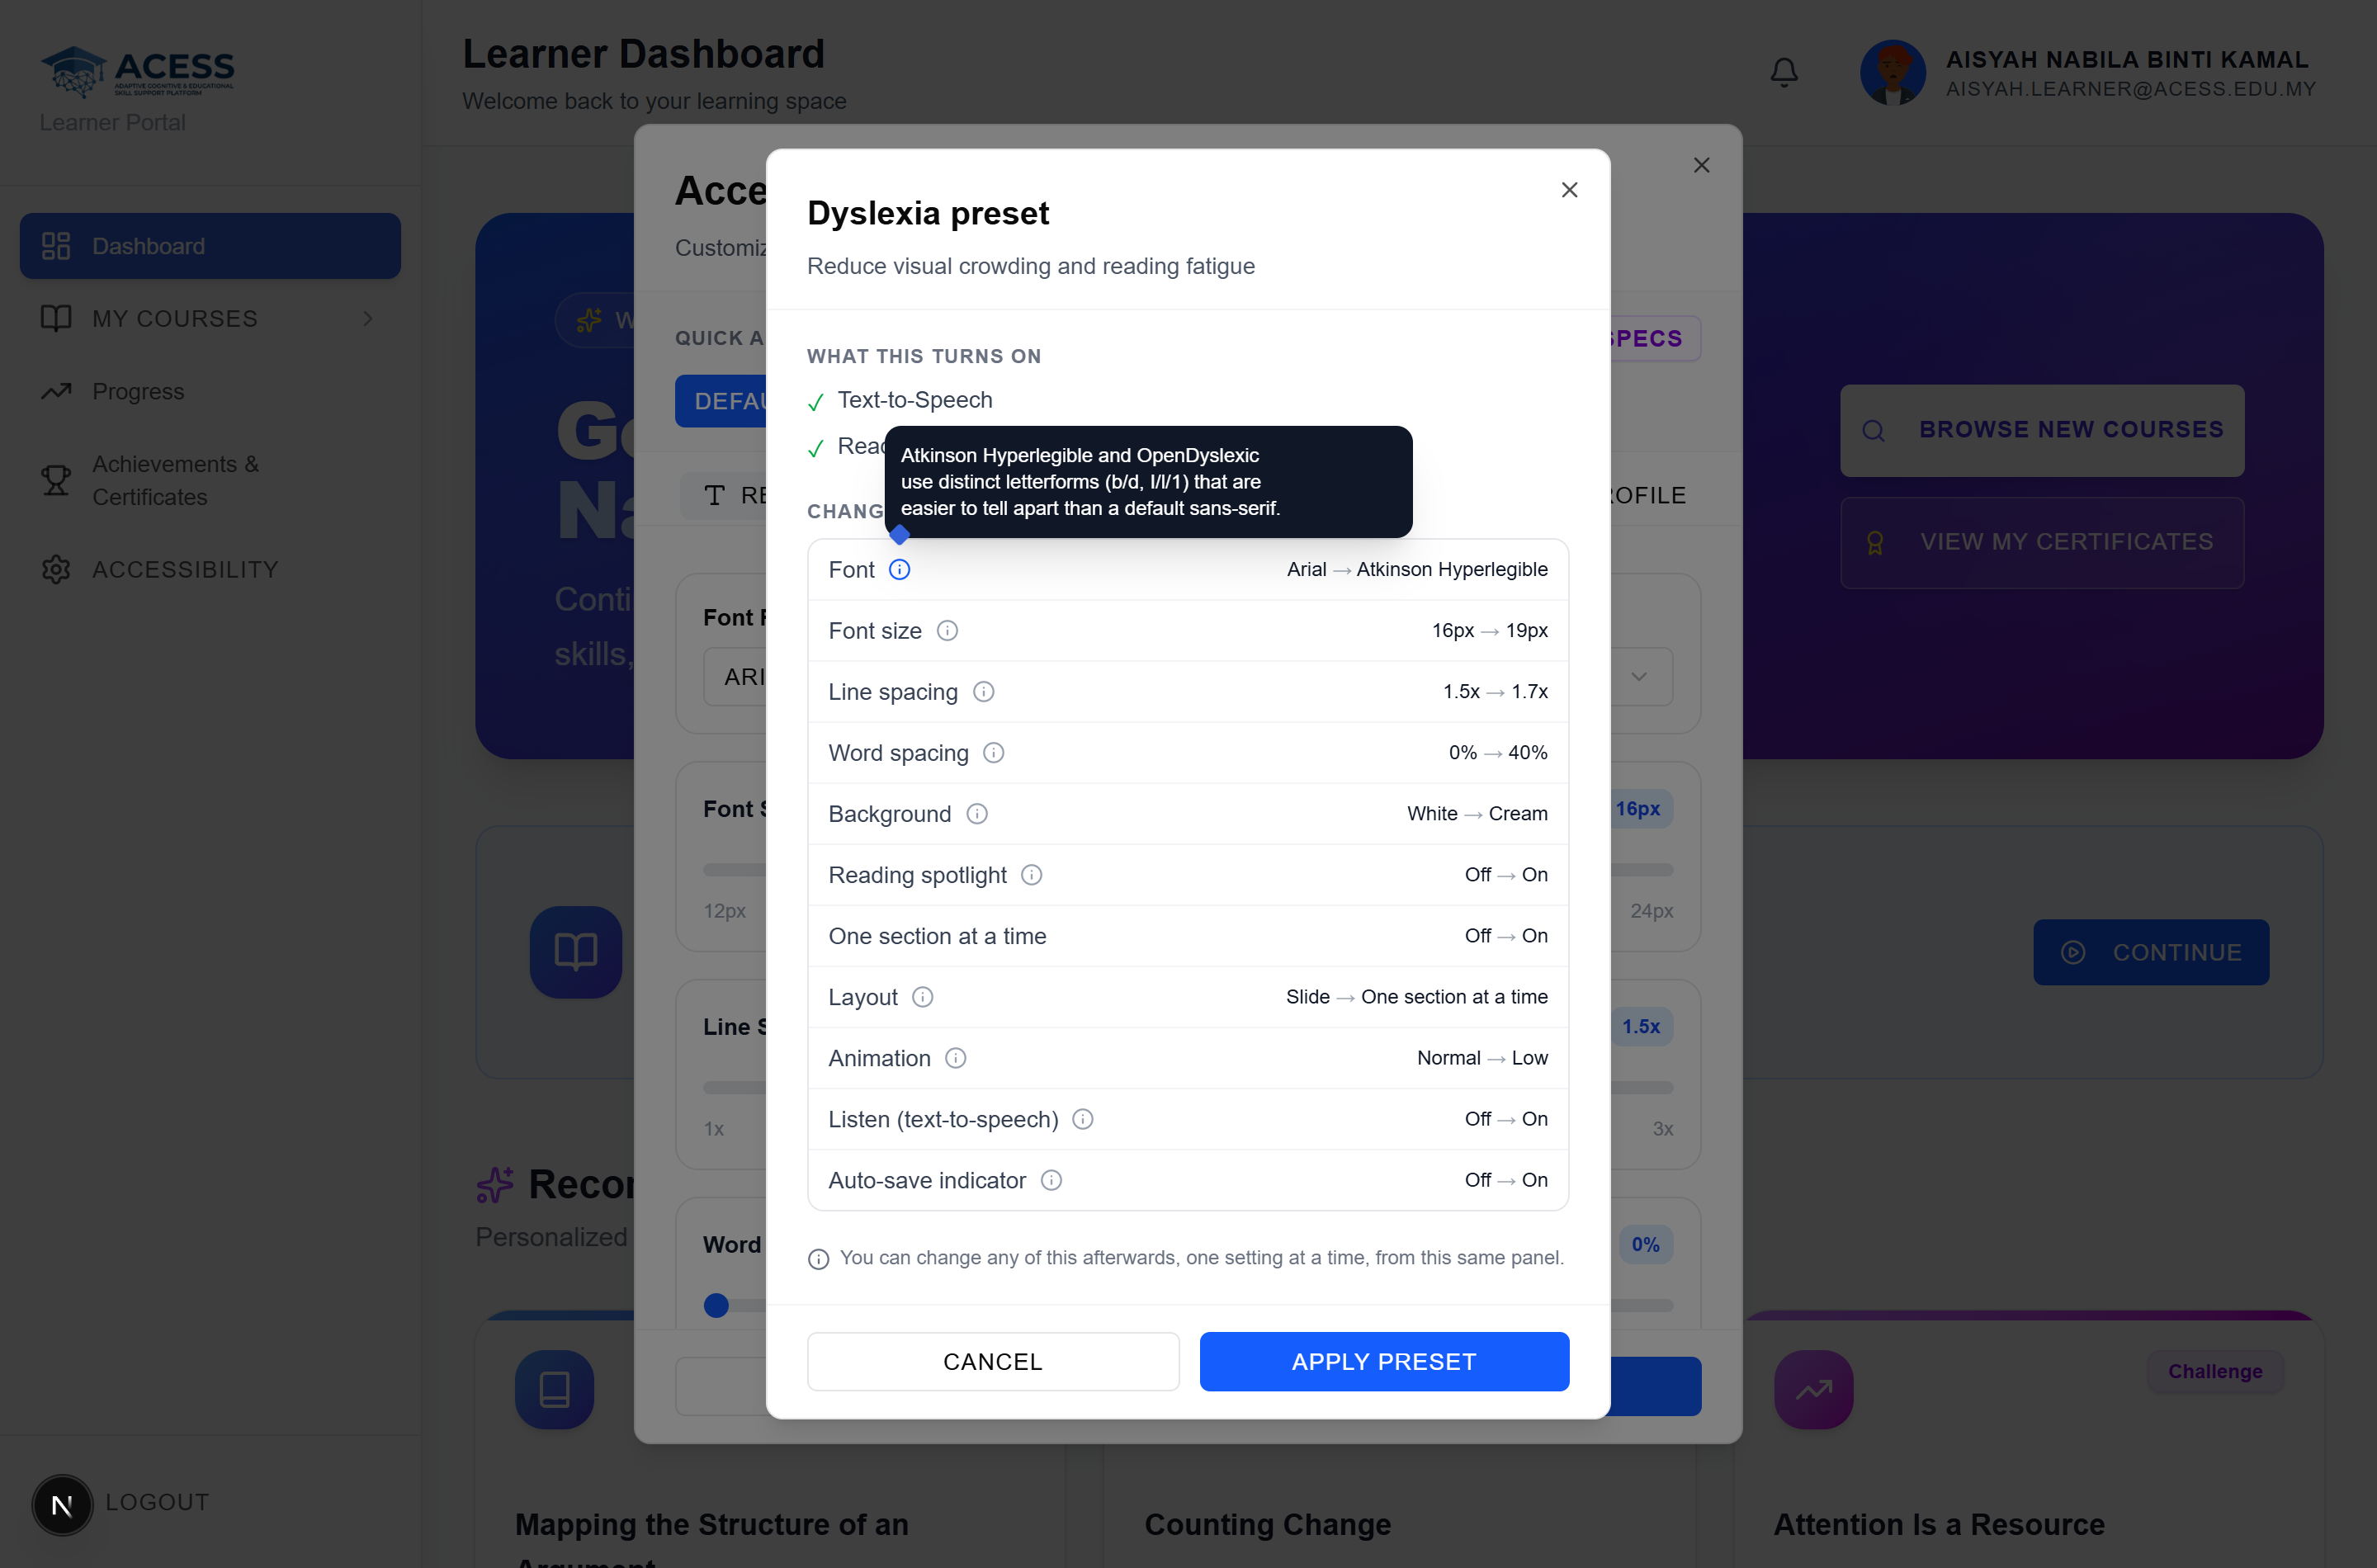
\includegraphics[width=0.86\textwidth]{Screenshots/a11y-preset-details.png}
\caption{Preset Preview Dialog}
\label{fig:preset_diff}
\end{figure}

\subsubsection{Effect of the presets on the lesson interface}

Figures~\ref{fig:preset_dyslexia} to \ref{fig:preset_autism} show the same lesson, viewed by the same learner account at the same window size, with only the accessibility preset changed between captures. The preset values in each case were applied by the platform itself and match Table~\ref{tab:preset_effects}, so the comparison shows what a learner selecting that preset actually receives.

\begin{figure}[htbp]
\centering
\begin{subfigure}{0.9\textwidth}
\centering
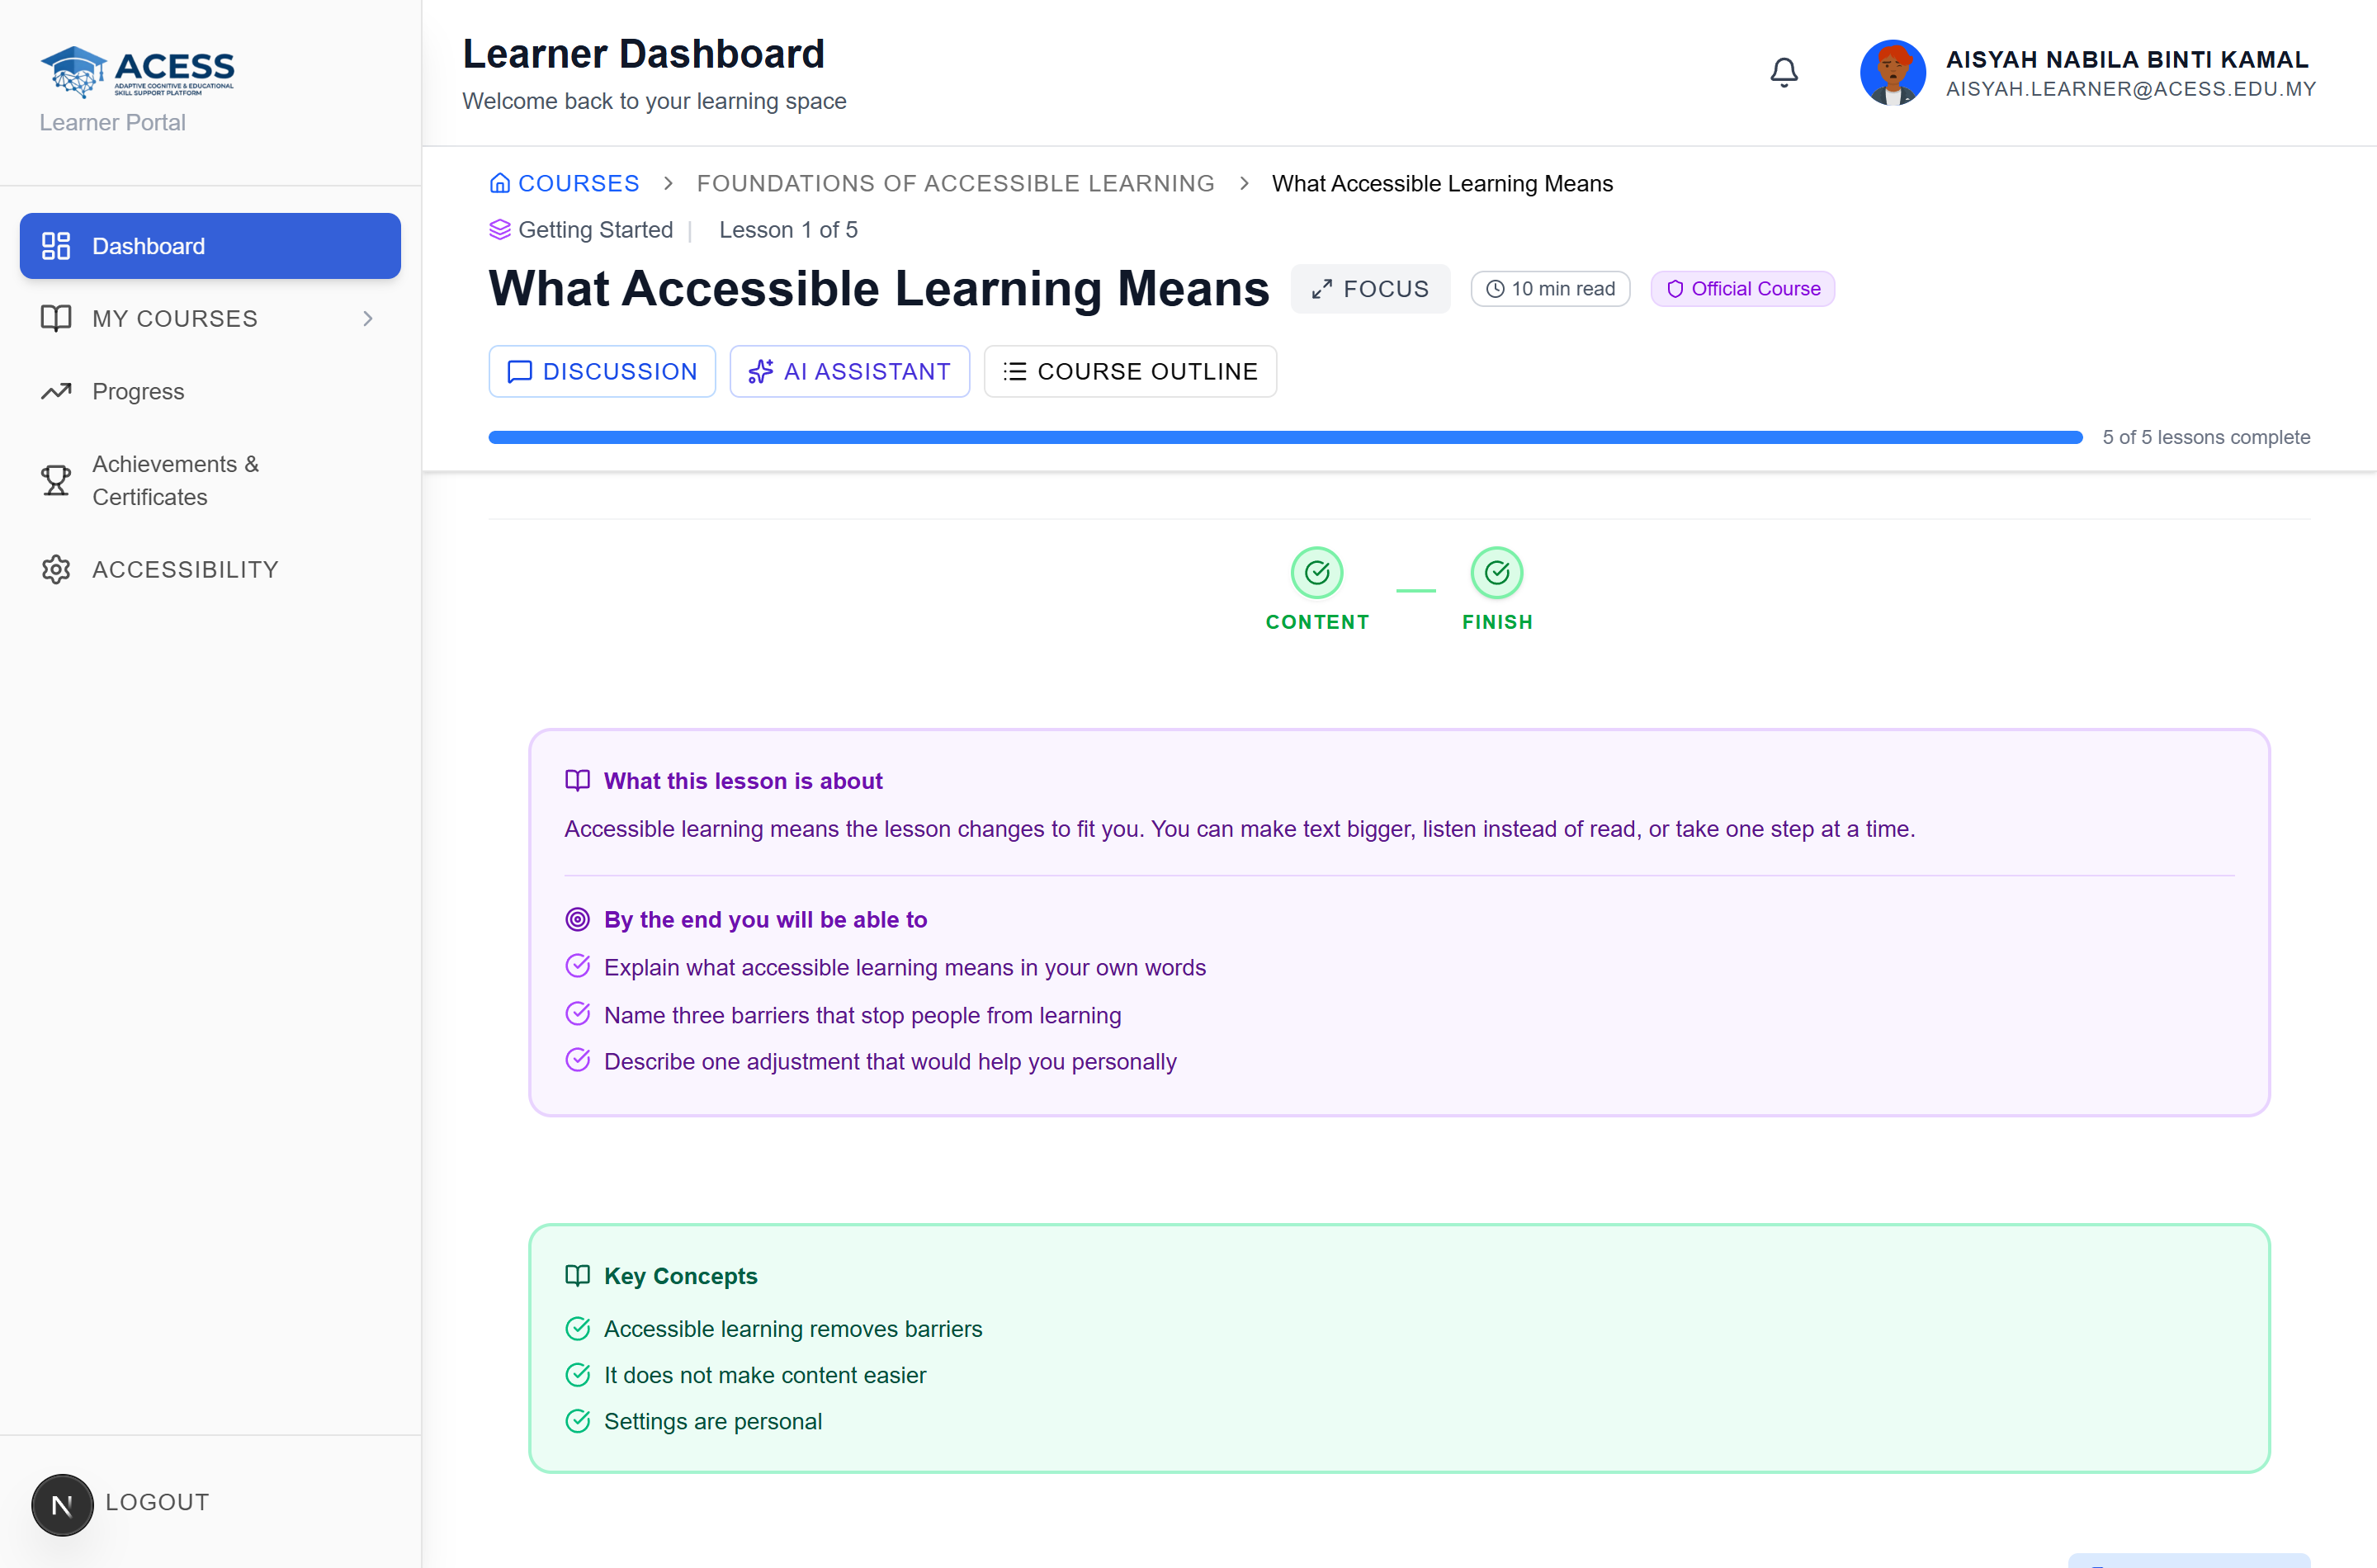
\includegraphics[width=\textwidth]{Screenshots/lesson-none.png}
\caption{Default}
\end{subfigure}

\vspace{4mm}
\begin{subfigure}{0.9\textwidth}
\centering
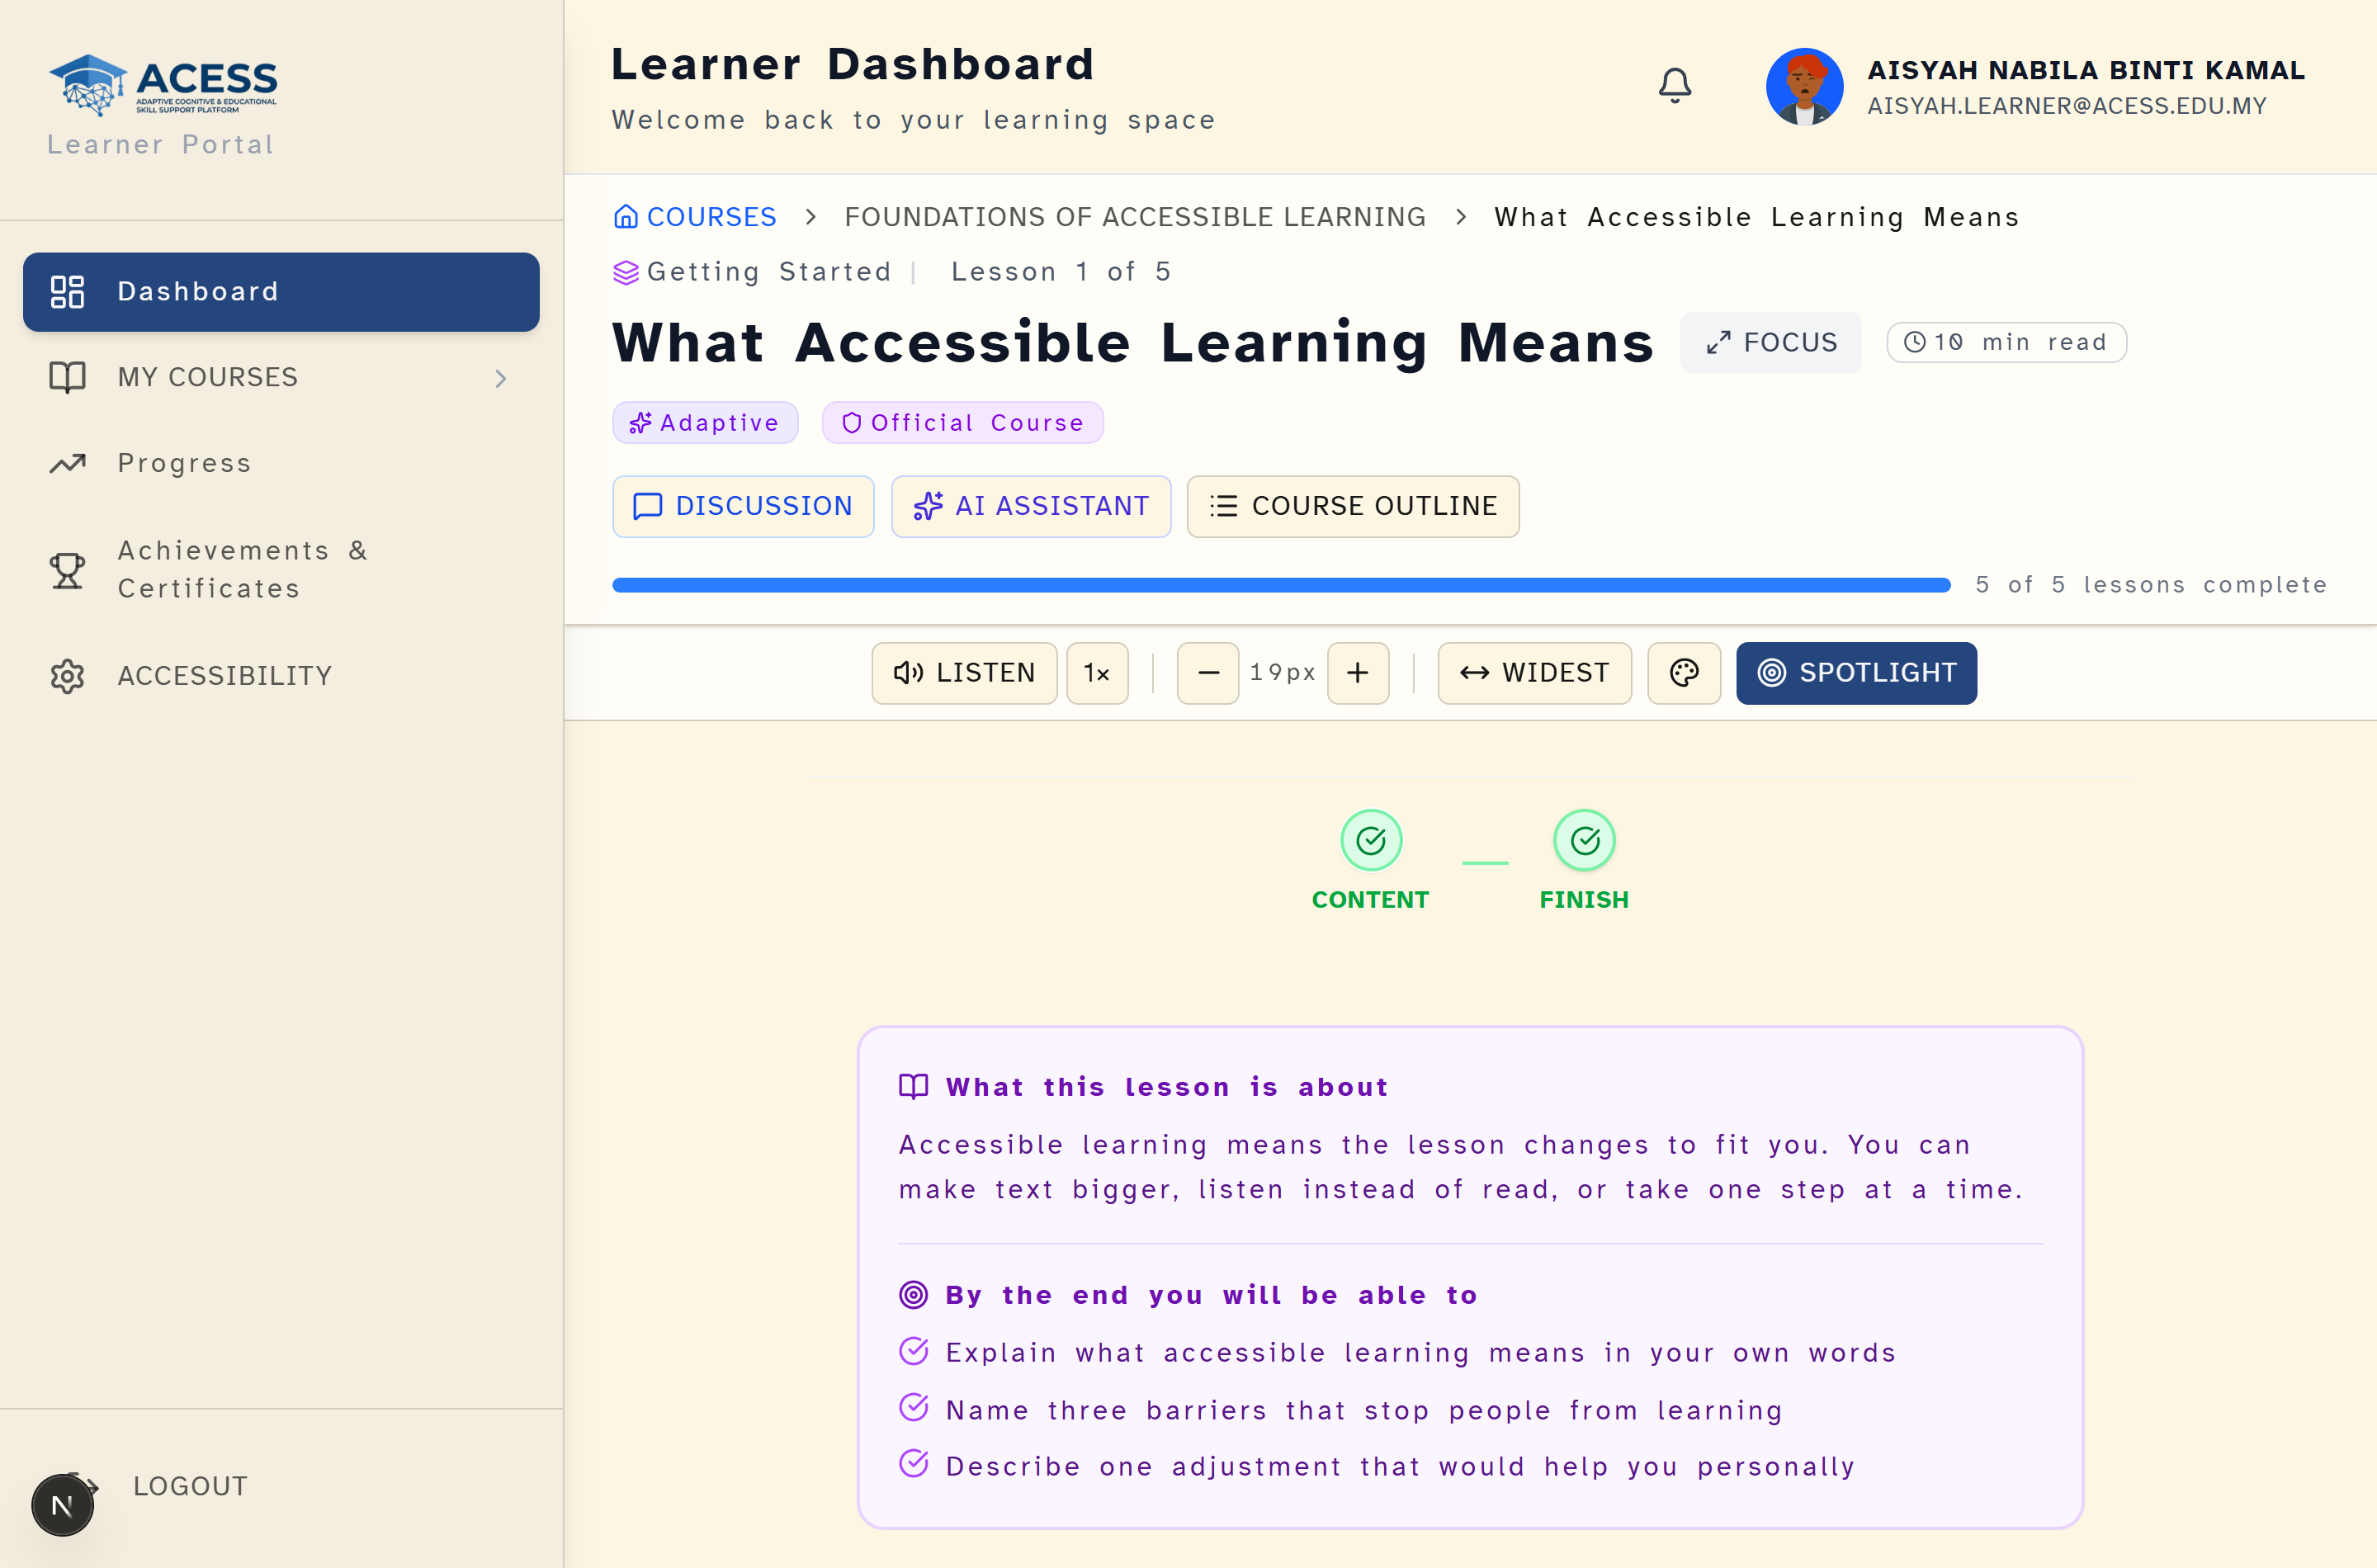
\includegraphics[width=\textwidth]{Screenshots/lesson-dyslexia.png}
\caption{Dyslexia preset}
\end{subfigure}
\caption{Lesson Interface: Default Compared with the Dyslexia Preset}
\label{fig:preset_dyslexia}
\end{figure}

Figure~\ref{fig:preset_dyslexia} shows the changes most readers would expect from an accessibility feature, namely typography and colour, together with two that are easy to miss. The reading column has narrowed rather than widened, because the limit is expressed in characters and the characters have become larger. A toolbar has also appeared below the lesson header carrying Listen, size, spacing, tint and spotlight controls, so that the learner can adjust the presentation without leaving the lesson to find a settings panel. Requiring a learner to navigate away in order to make reading easier would itself be a barrier.

\begin{figure}[htbp]
\centering
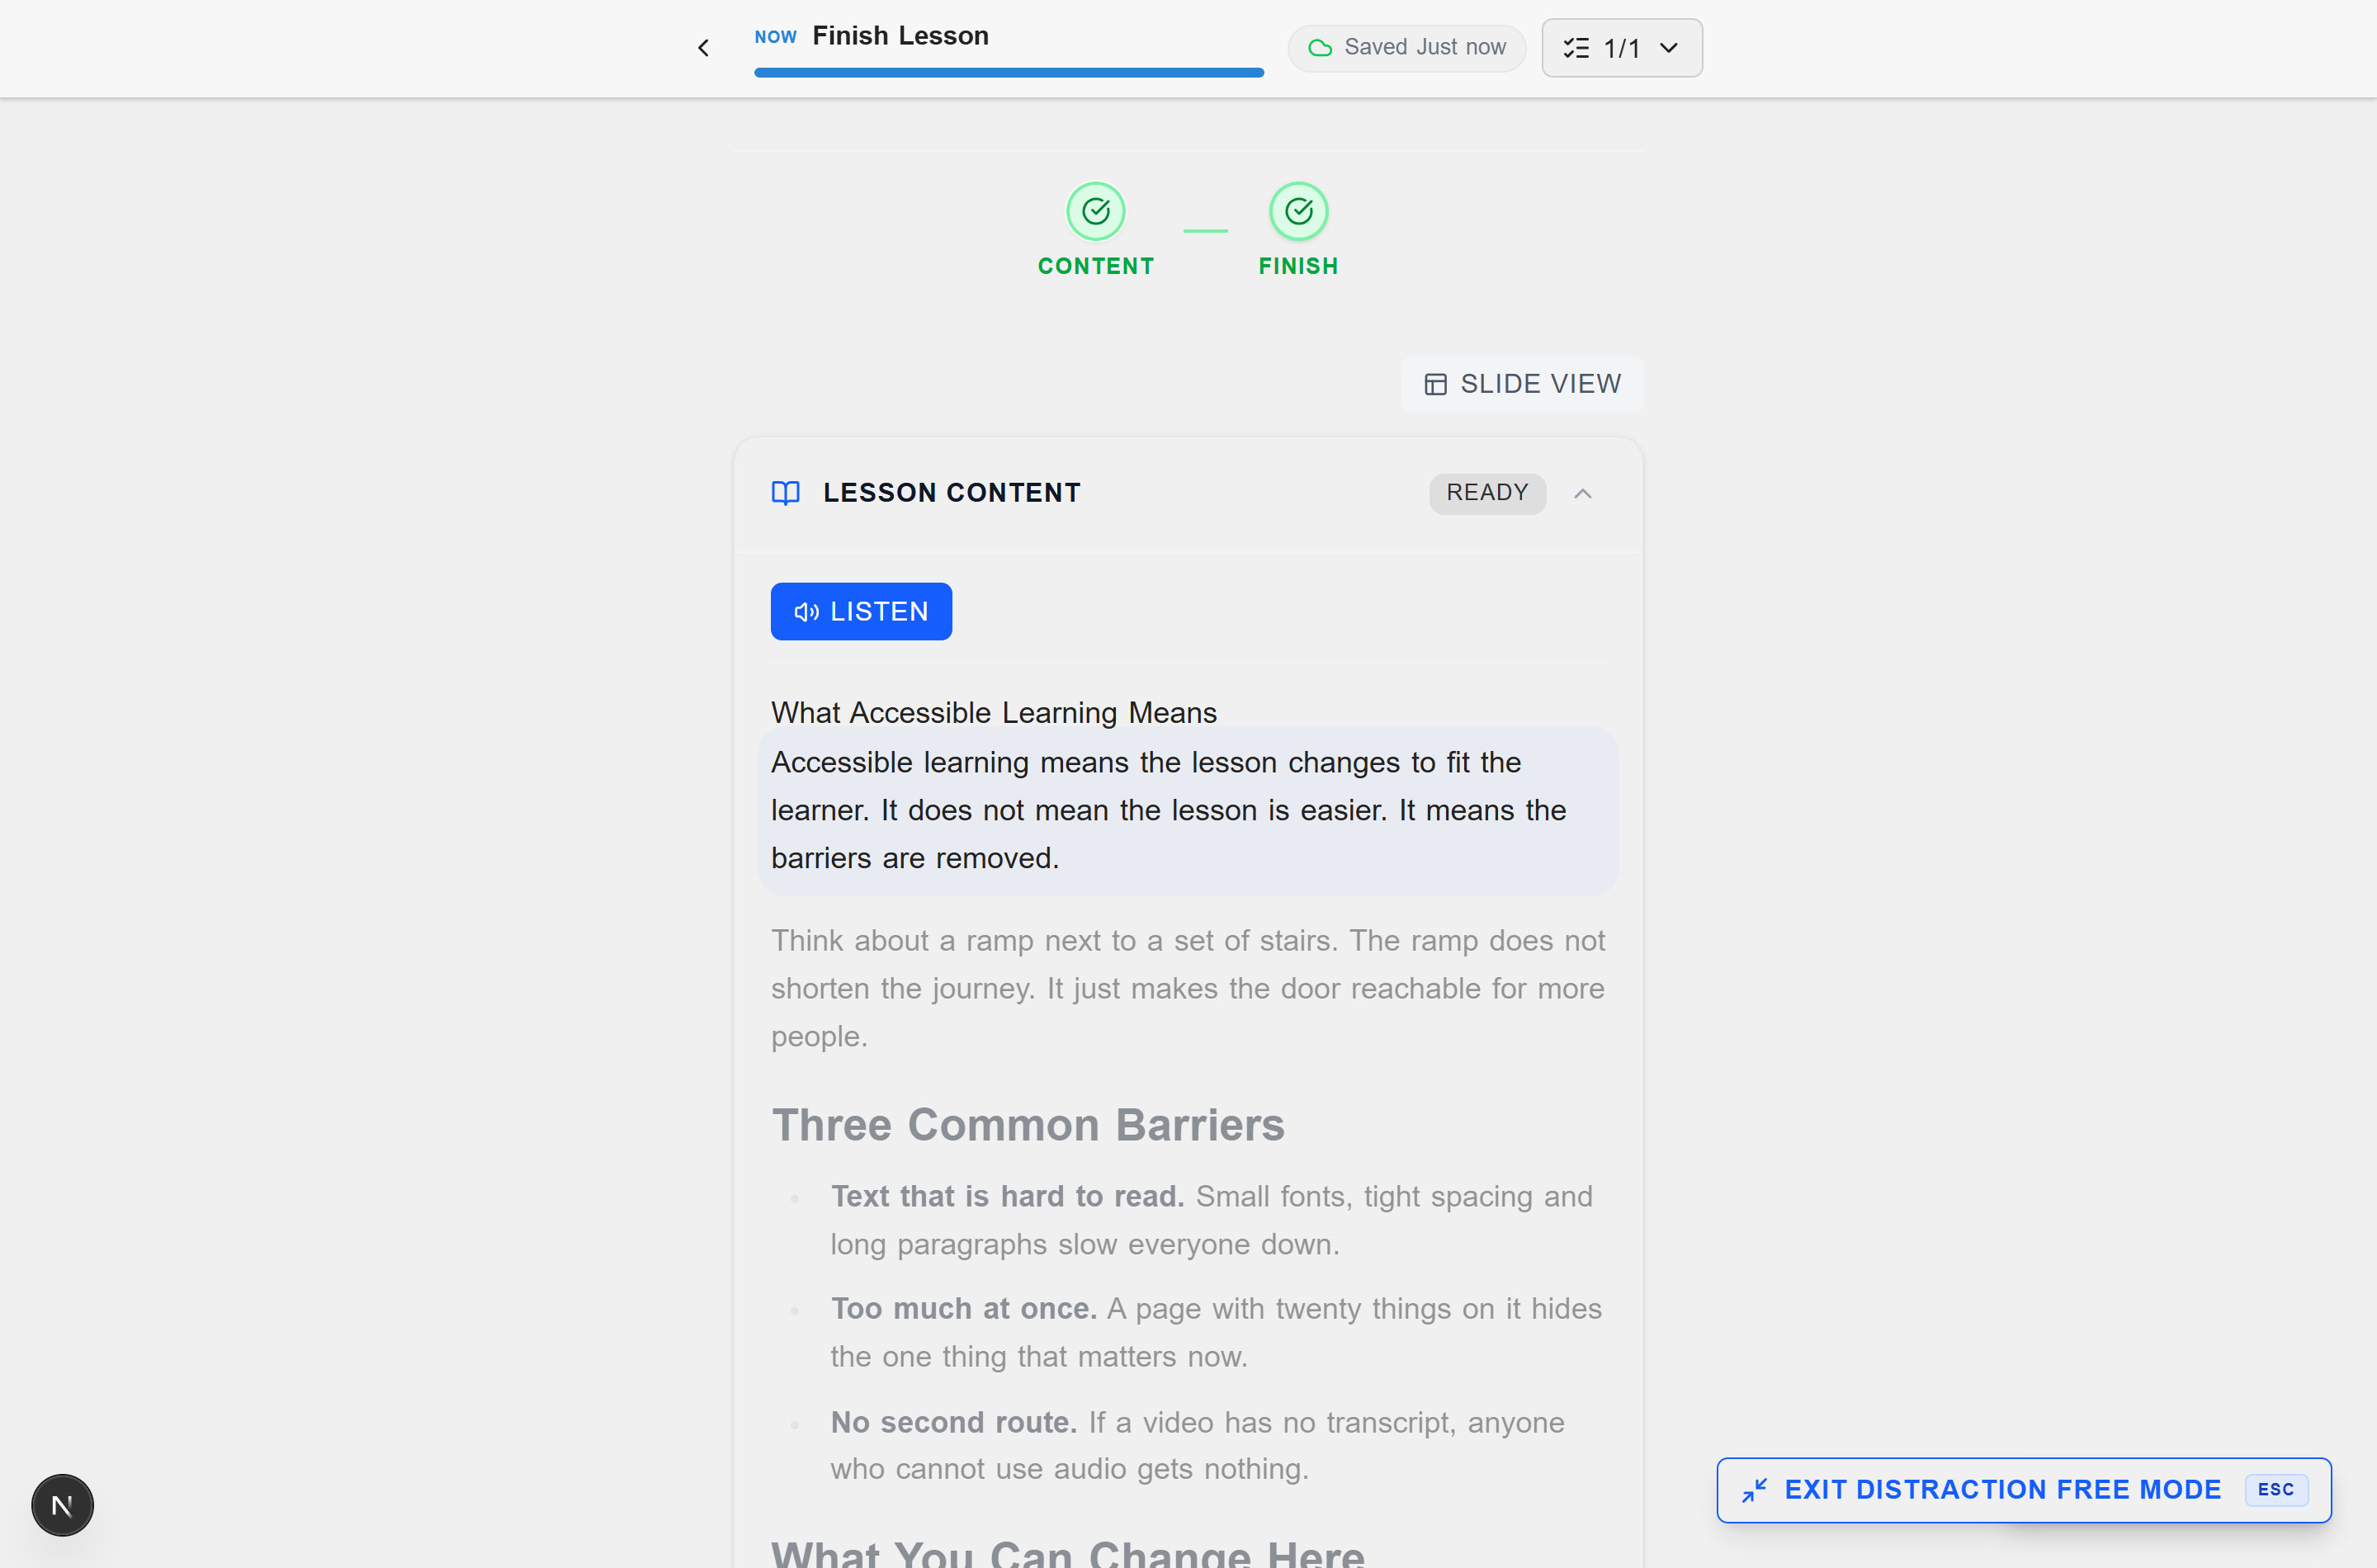
\includegraphics[width=0.92\textwidth]{Screenshots/lesson-adhd.png}
\caption{Lesson Interface Under the ADHD Preset}
\label{fig:preset_adhd}
\end{figure}

Figure~\ref{fig:preset_adhd} illustrates the difference between hiding elements and supporting attention. The sidebar and notification area are removed, a persistent bar carries the current task together with an auto-save indicator, and the reading spotlight dims every paragraph except the one in focus. Everything competing for attention has gone, but the reading column has not expanded to fill the space and remains bounded at 66 characters. An exit control in the lower right, and the keyboard shortcut it advertises, ensure that the mode is never a trap.

\begin{figure}[htbp]
\centering
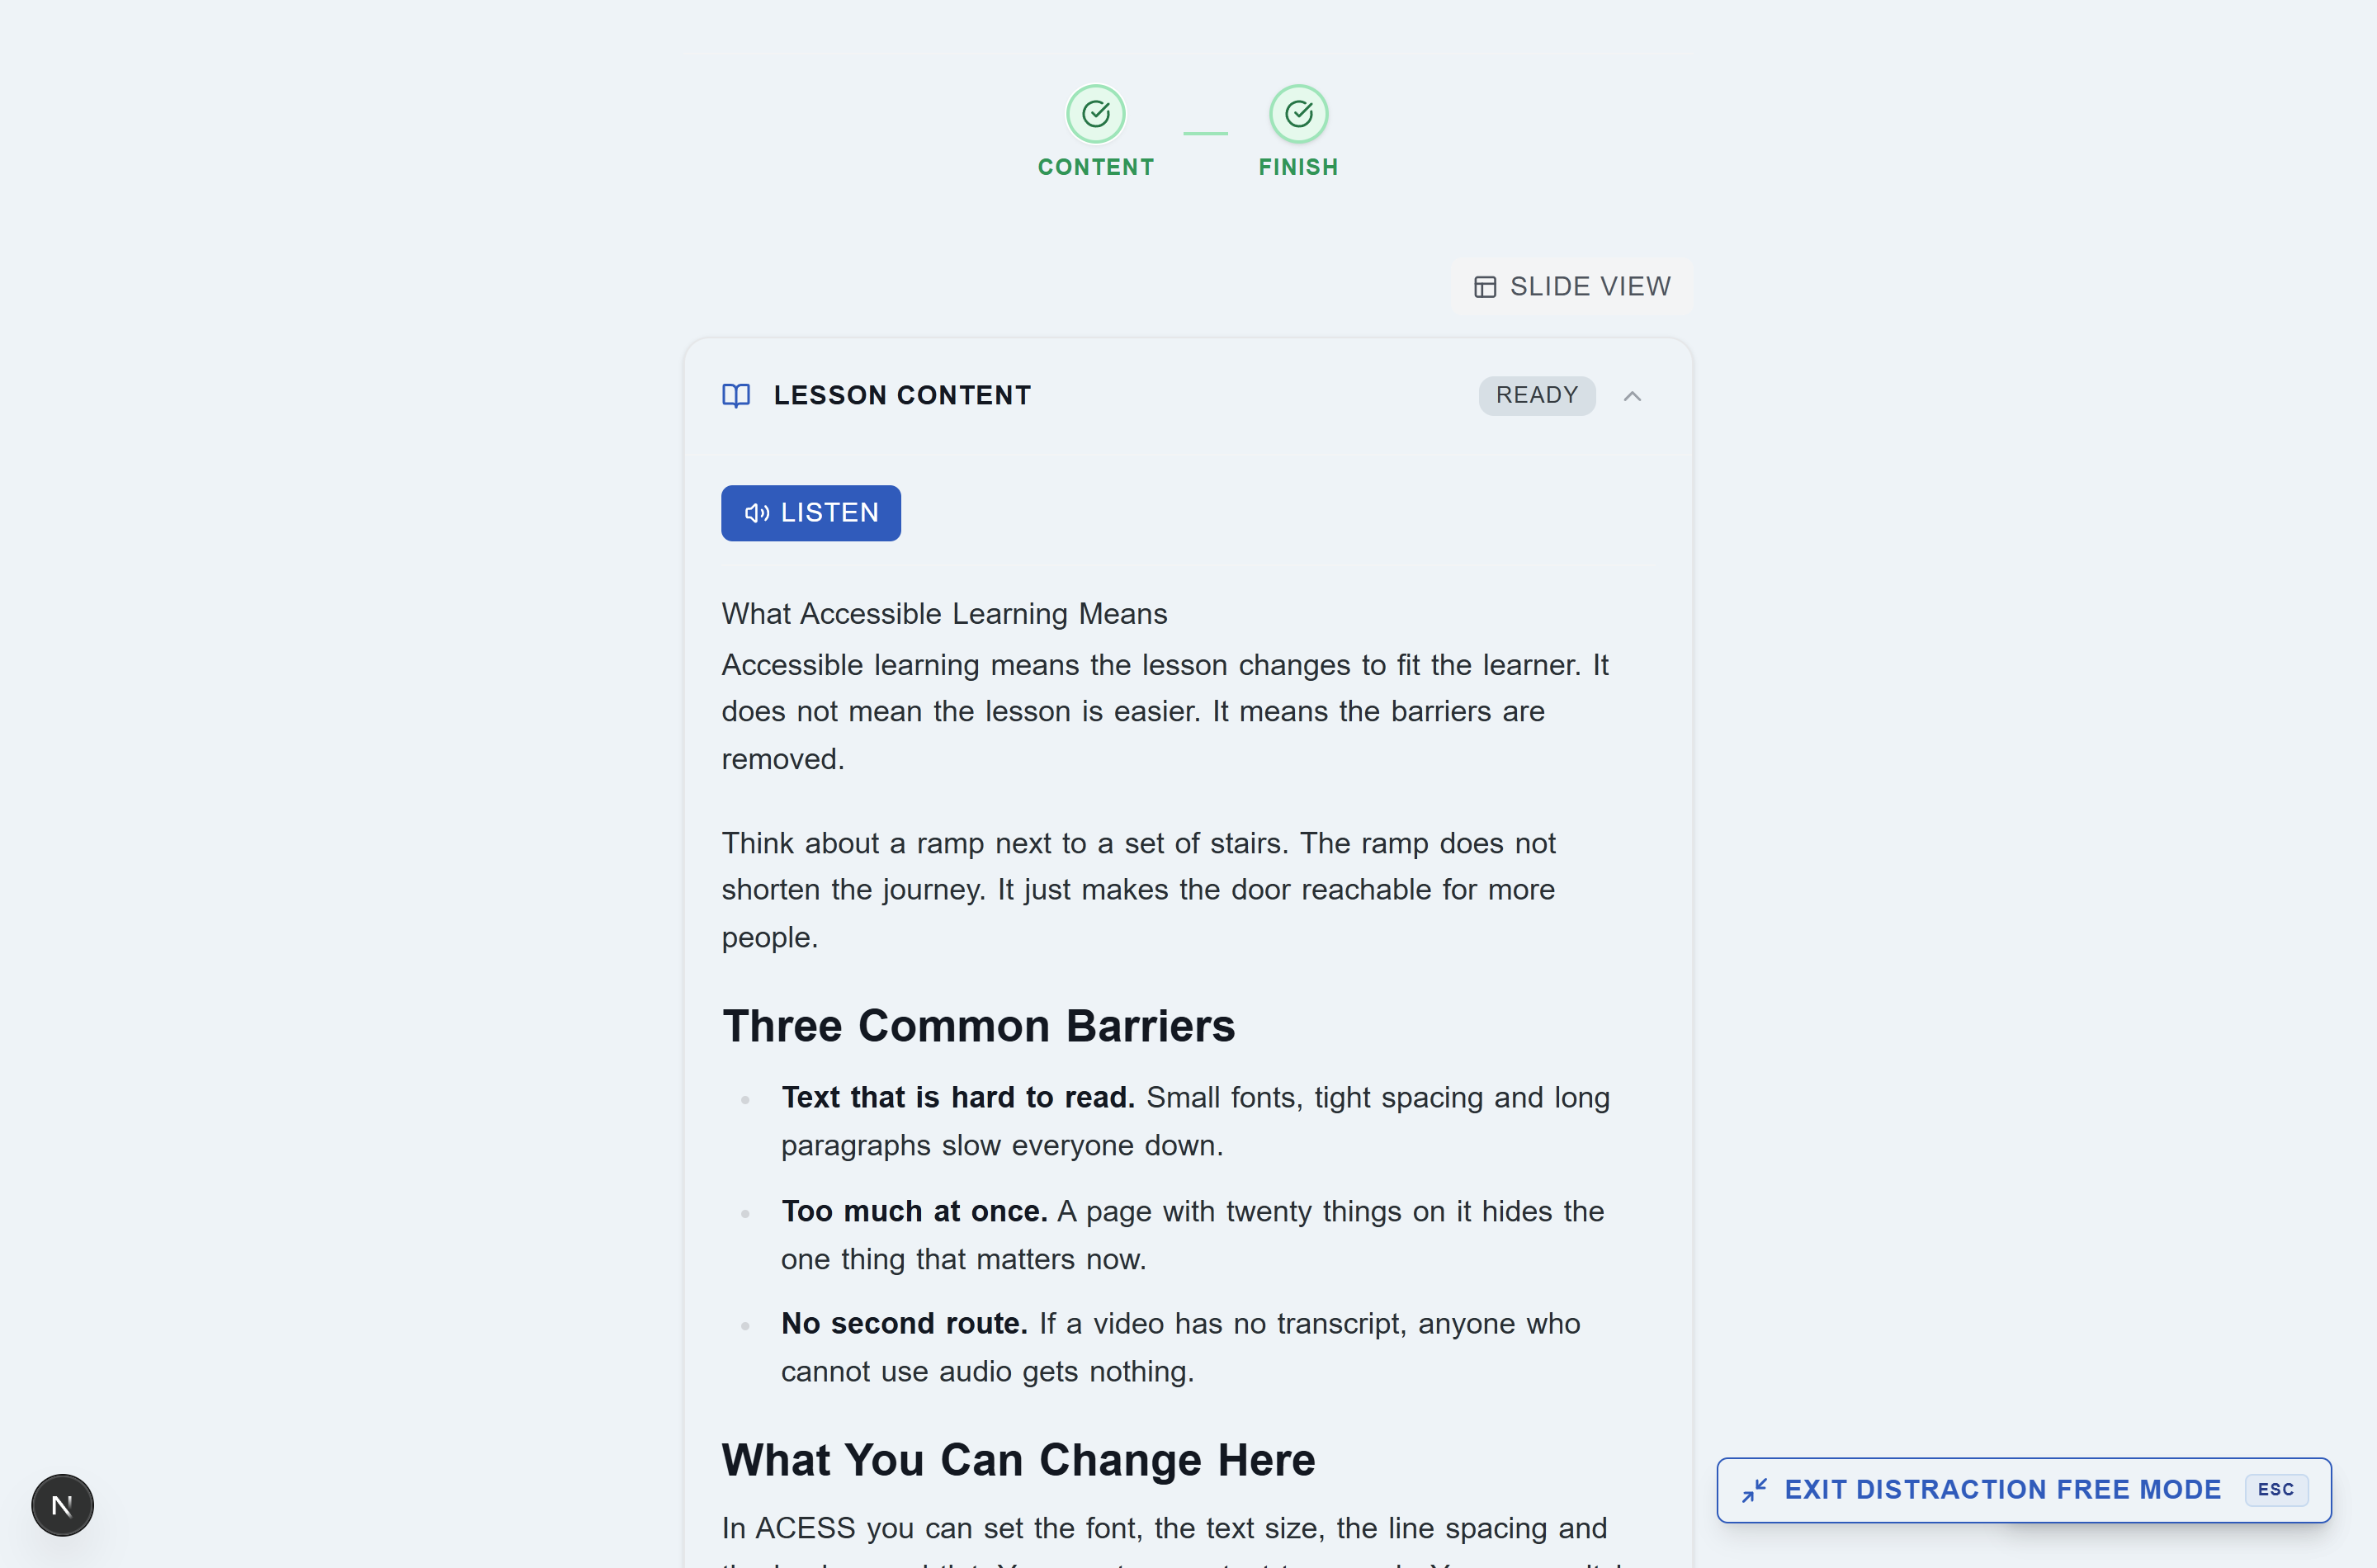
\includegraphics[width=0.92\textwidth]{Screenshots/lesson-autism.png}
\caption{Lesson Interface Under the Autism Preset}
\label{fig:preset_autism}
\end{figure}

Figure~\ref{fig:preset_autism} shows the least visually dramatic and most structurally significant of the three, with its pale blue background, reduced colour saturation and motion removed. The substantive change is that the phases of the lesson are shown as an explicit sequence above the content, which tells the learner what the lesson consists of and how far through it they are before they begin. The reading width is deliberately not narrowed here: unlike Dyslexia, where a narrow measure assists decoding, the need addressed by this profile is predictability, and keeping the default width means the page does not change shape when the learner moves between courses.

Figure~\ref{fig:ui_lesson_dyslexia} shows the effect at dashboard rather than lesson level, where the Dyslexia preset replaces the multi-column card grid of Figure~\ref{fig:ui_learner_dashboard} with a single-column list and enlarges the navigation.

\begin{figure}[htbp]
\centering
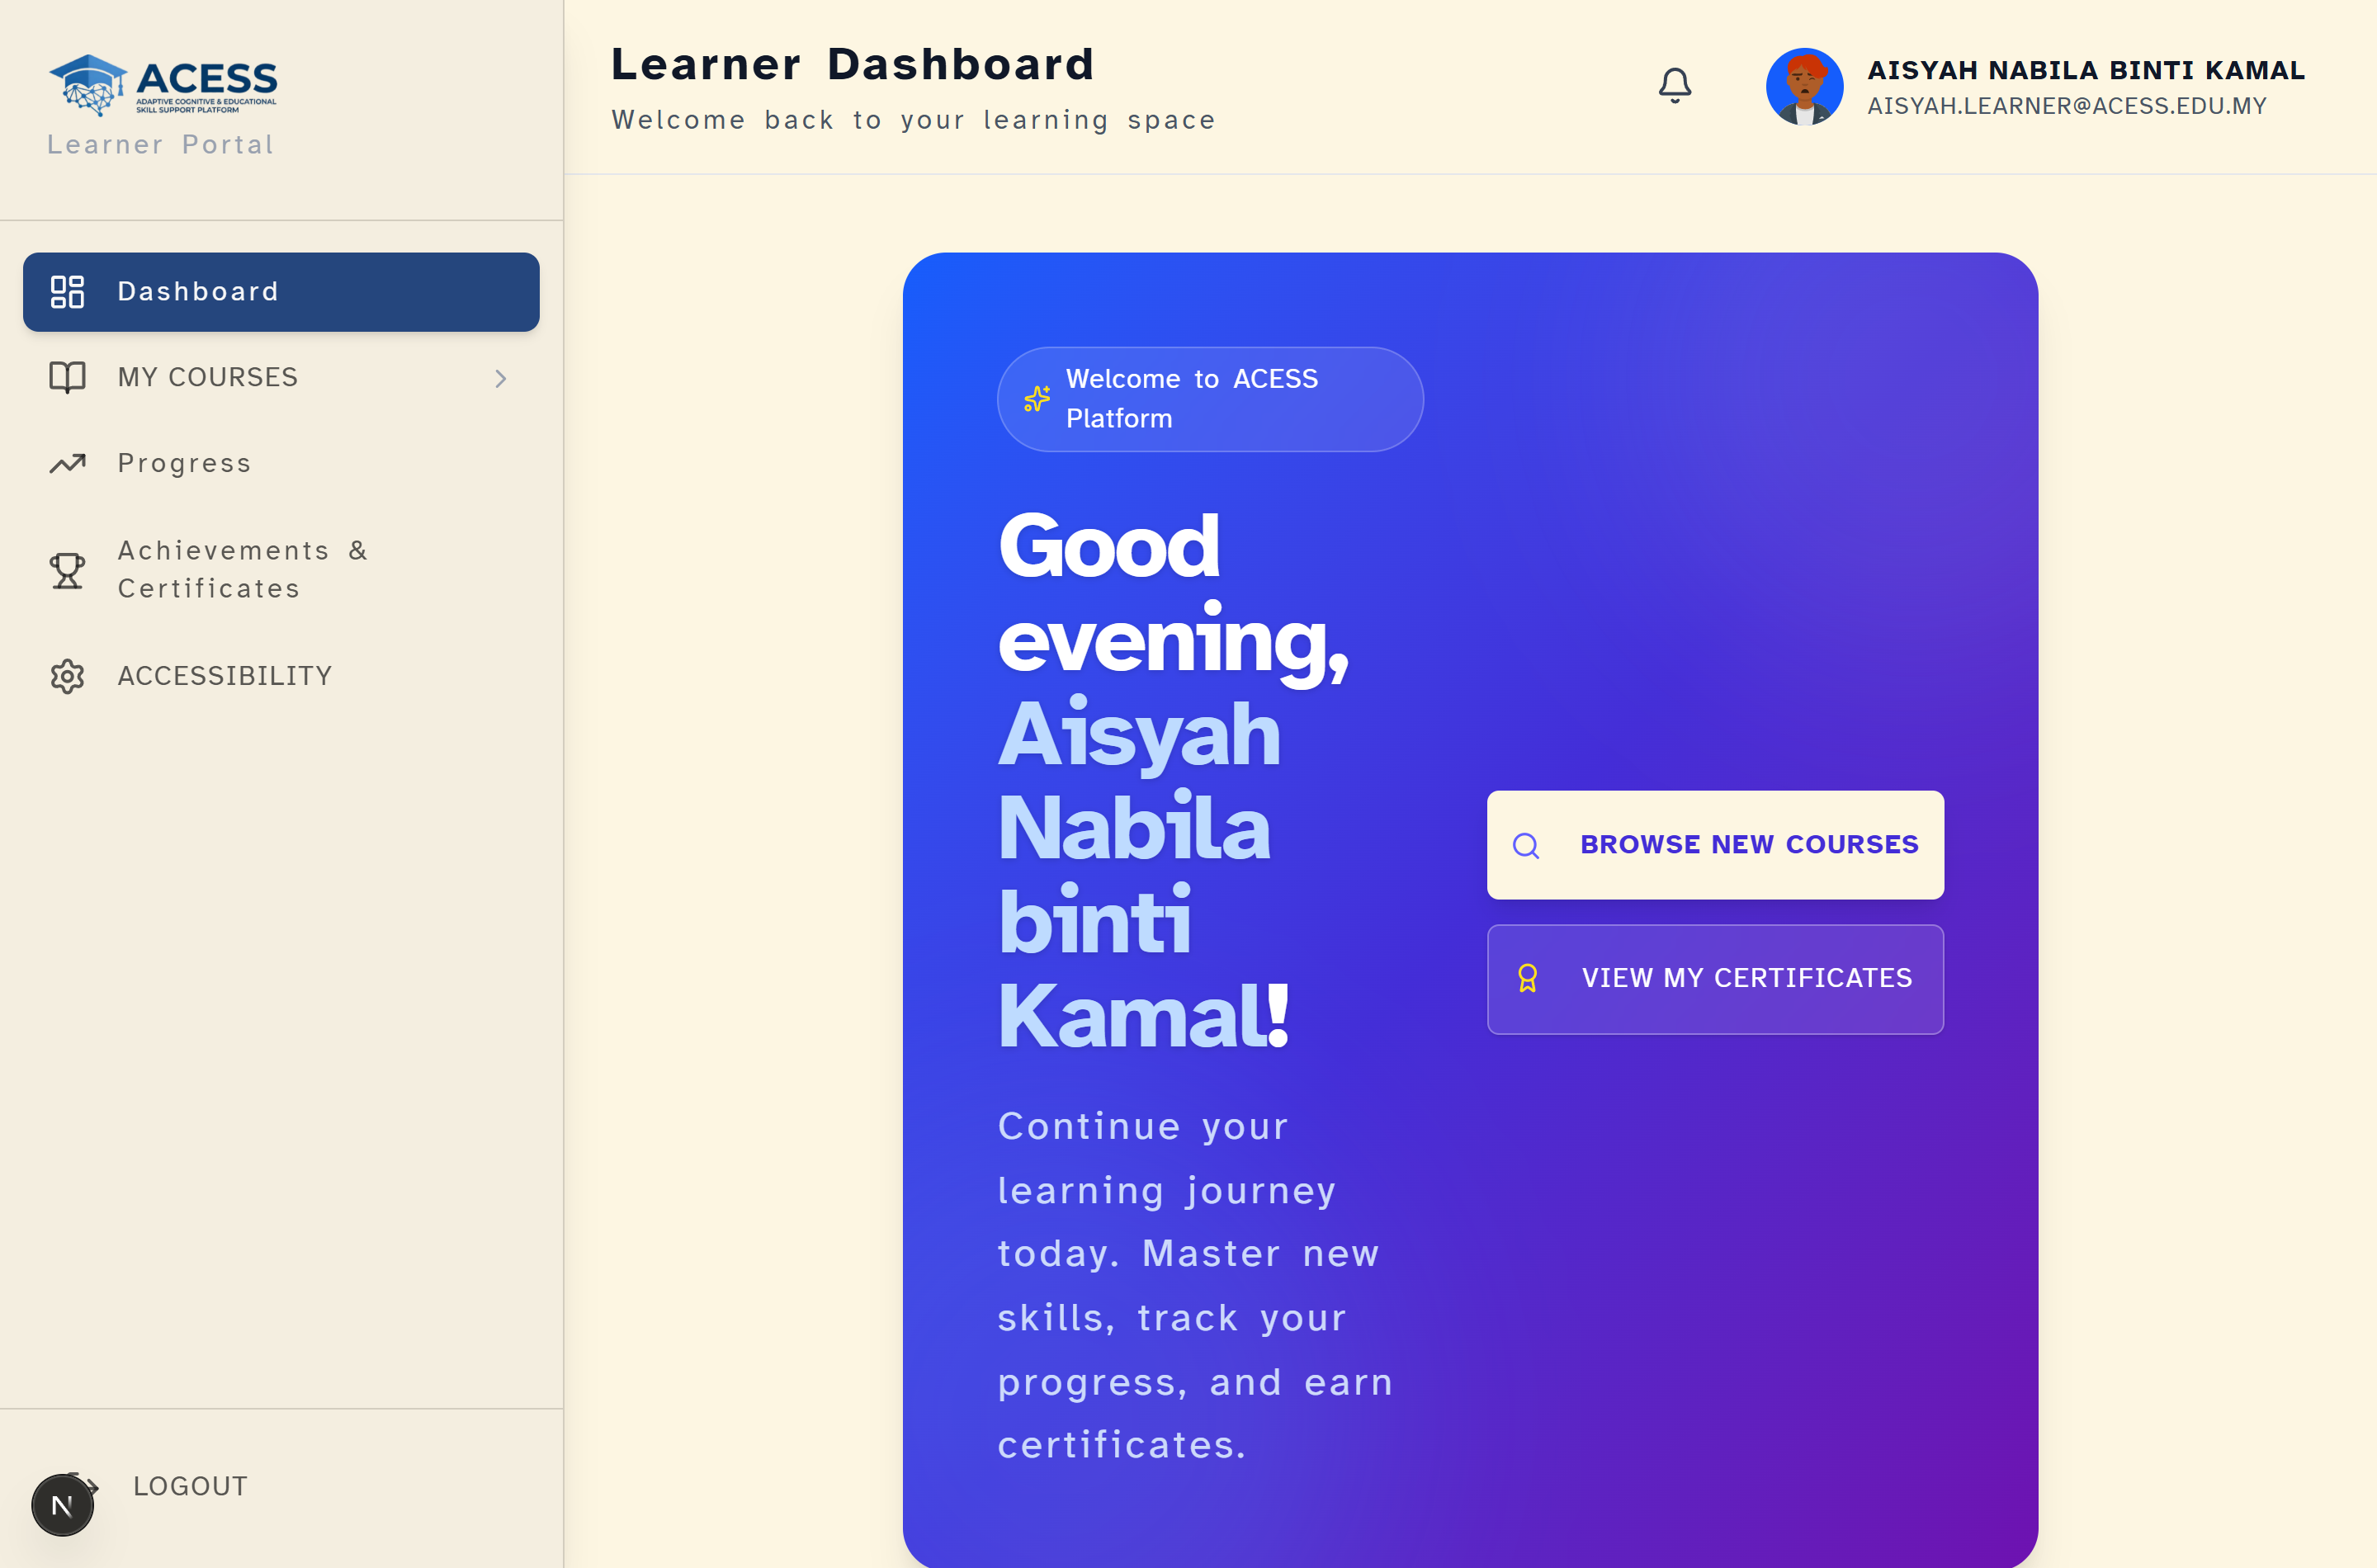
\includegraphics[width=0.92\textwidth]{Screenshots/dashboard-dyslexia.png}
\caption{Learner Dashboard Under the Dyslexia Preset}
\label{fig:ui_lesson_dyslexia}
\end{figure}

\subsubsection{Authoring-time accessibility compliance checking}
\label{sec:a11y-audit}

The content criteria identified in Section~\ref{sec:a11y-design} cannot be met by the platform on the educator's behalf. ACESS therefore provides a compliance checker that evaluates a lesson while it is being written.

The checker has three properties that make its output defensible. It is deterministic: every rule is a fixed threshold with a published source, so the same lesson always produces the same score. It has no side effects and runs immediately, which is why the same engine can be used both against the unsaved draft in the editor and against saved lessons for the course-level report, with the two necessarily agreeing. And it is profile-aware: a baseline of seven rules applies to every lesson, with a further set added according to the accessibility focus declared for the course (six for ADHD, five for Autism and seven for Dyslexia), so an educator writing for learners with Dyslexia is checked on sentence length and readability while one writing for autistic learners is checked on figurative language and stated objectives.

Rules that cannot apply are marked as not applicable rather than failed and are excluded from the score, so a lesson with no video is not penalised for lacking a transcript. The score is the weighted proportion of applicable rules passed, reported as critical below 50, warning below 80, and good at 80 or above.

\begin{figure}[htbp]
\centering
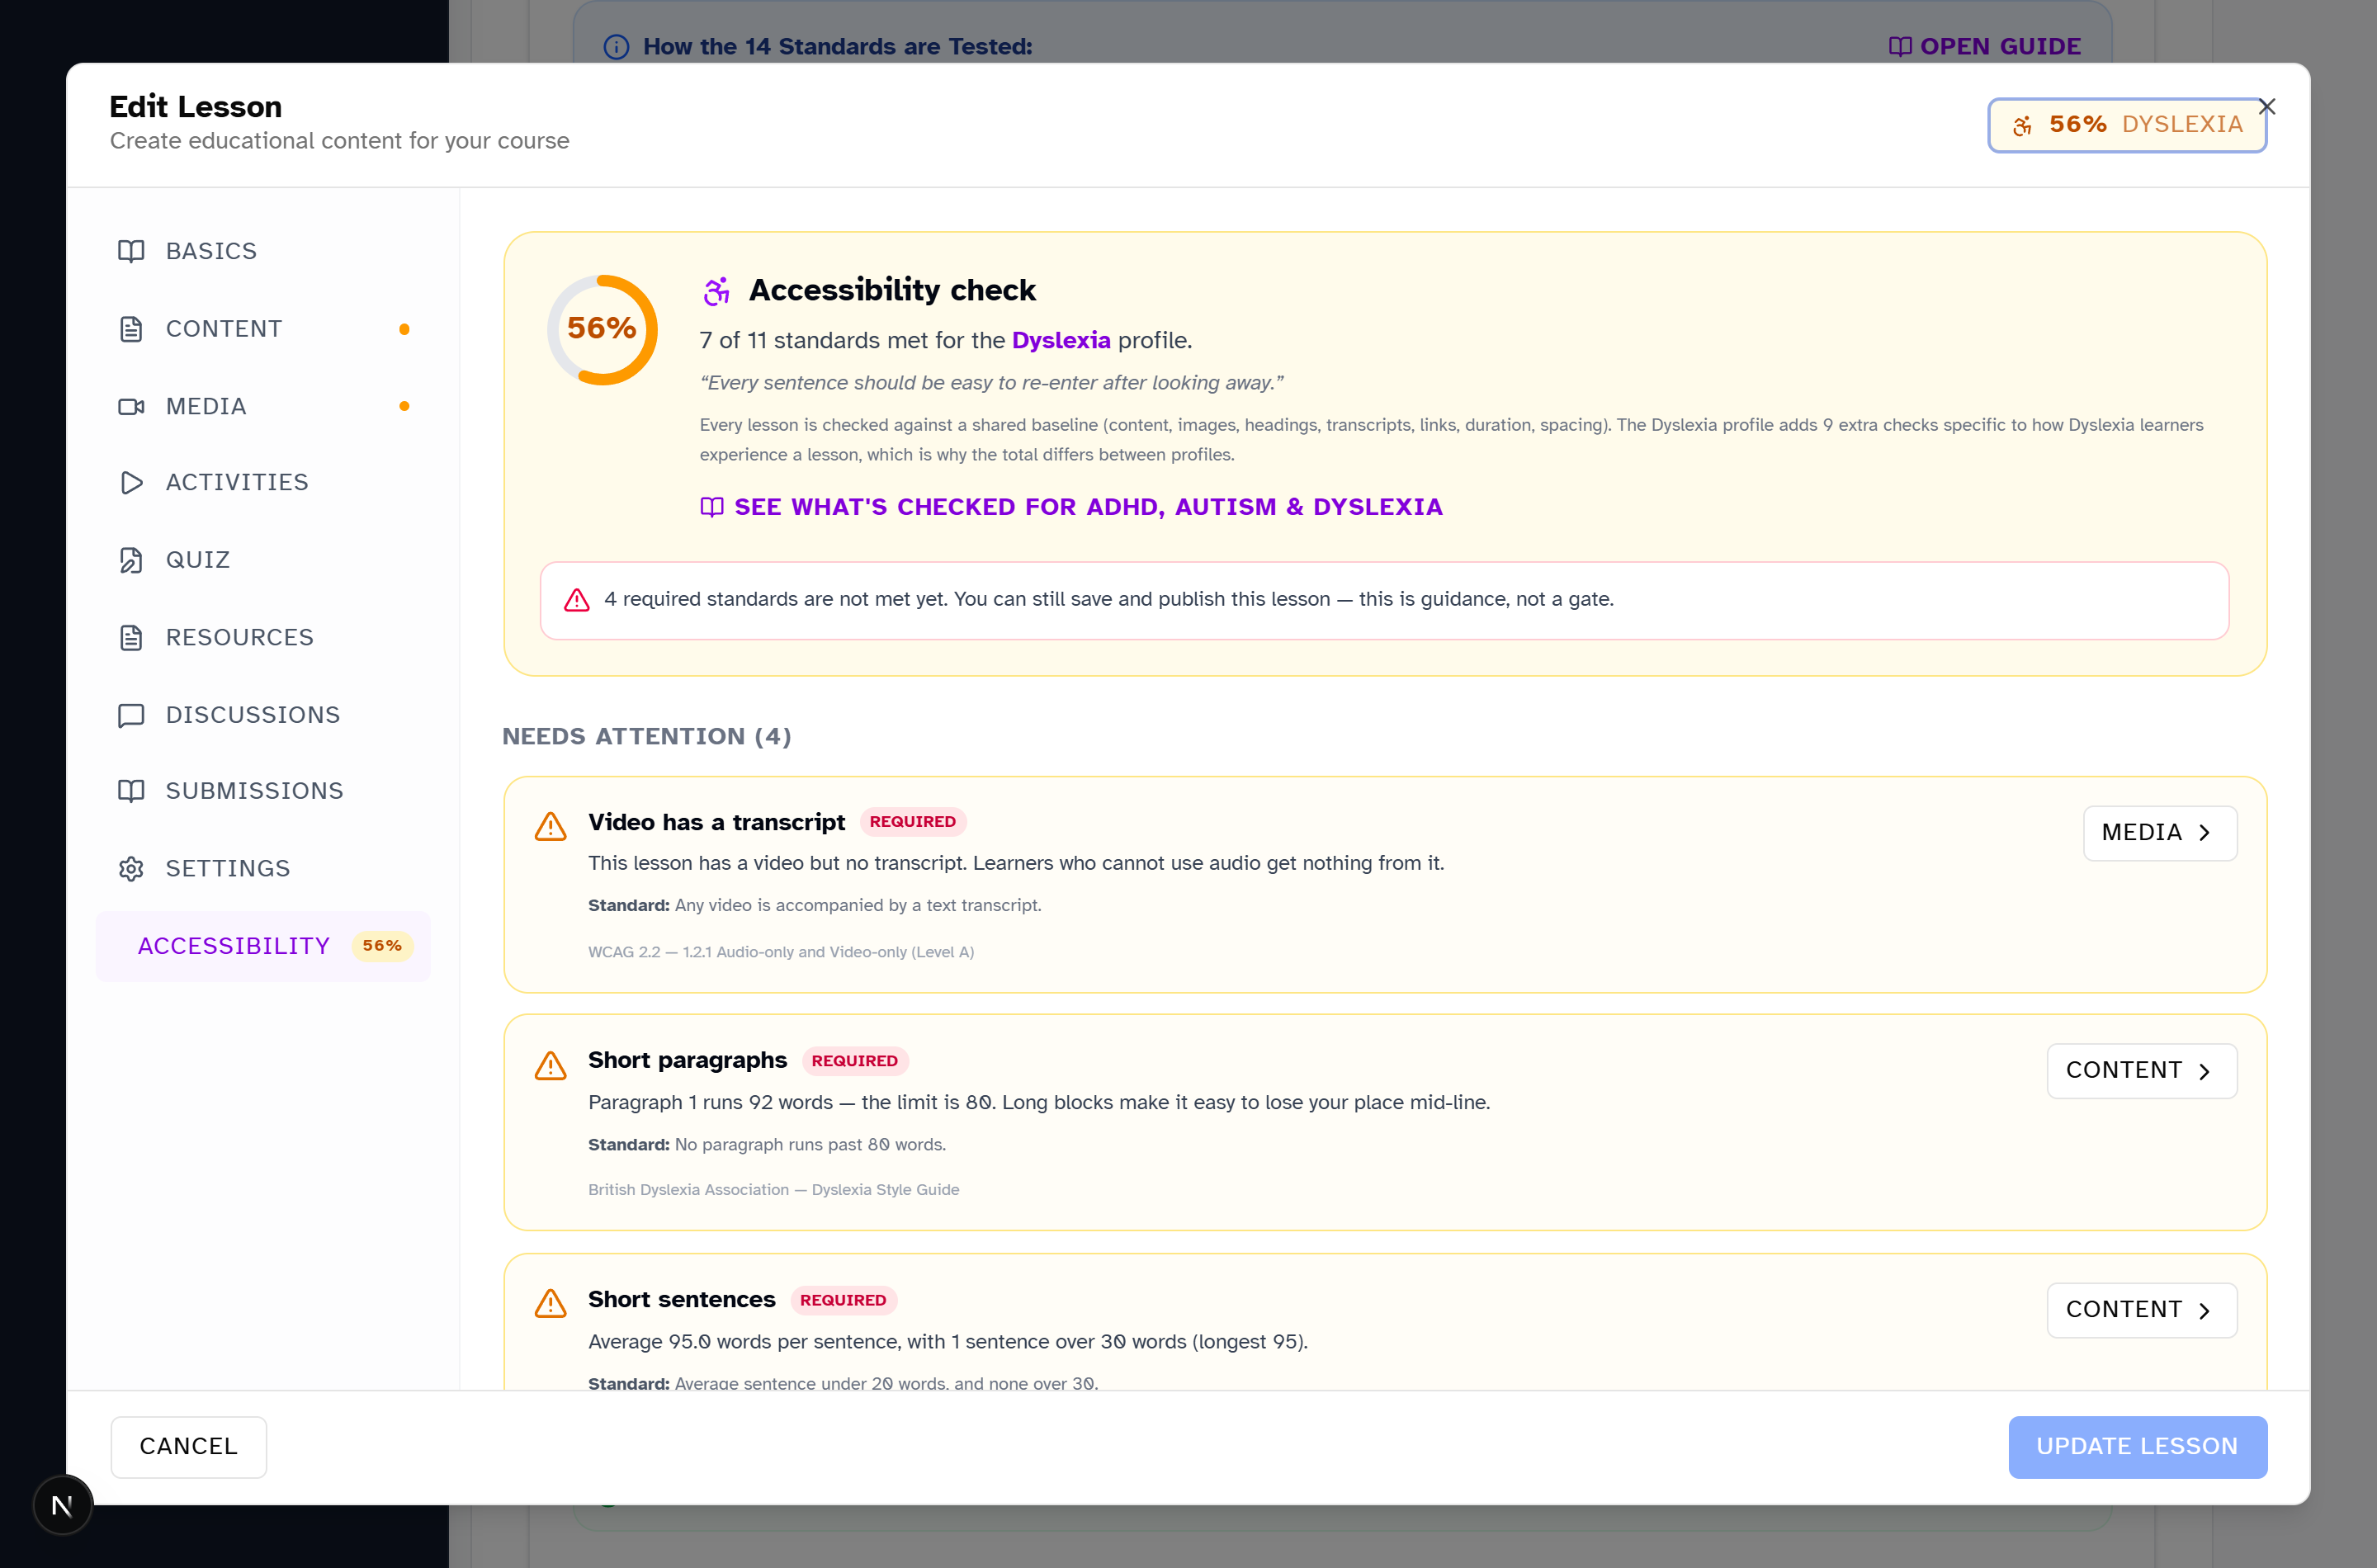
\includegraphics[width=0.94\textwidth]{Screenshots/educator-a11y-compliance.png}
\caption{Lesson Accessibility Check in the Educator Editor}
\label{fig:ui_edu_a11y}
\end{figure}

Figure~\ref{fig:ui_edu_a11y} shows the checker reporting on a lesson from the demonstration dataset. Three properties of that output distinguish it from a generic accessibility linter. Each finding states the measured value rather than only that a rule failed, so it reads, for example, that a paragraph runs 92 words against a limit of 80. Each finding names its source, so an educator who disagrees can consult the standard rather than the tool. And each finding provides a route to the correction, opening the editor tab that owns the problem.

The panel also states, in the same view, that unmet standards remain and that the lesson can still be saved and published. This is a deliberate policy choice. A publication gate would encourage educators to satisfy the rule rather than the reader, for example by padding a summary to clear a word count, and would position accessibility as an obstacle to teaching. The checker advises and the educator decides; what the platform guarantees is that the decision is an informed one.

The same engine runs at course level, aggregating the fourteen standards that apply across a whole course and identifying which lessons are responsible for each unmet one, so that an educator can distinguish a single weak lesson from a course-wide problem.

\subsubsection{Known accessibility gaps}
\label{sec:a11y-gaps}

The following are real limitations of the current build, and each is disclosed on the platform's own accessibility statement as well as here.

\begin{enumerate}
    \item \textbf{No assistive technology has been tested against this build.} No screen reader or other assistive technology has been used with ACESS. Every claim in Table~\ref{tab:wcag_map} is verified by inspecting the code that implements it and by operating the interface in a browser, not by using it as a screen-reader user would. This is the most significant limitation in this chapter.
    \item \textbf{No neurodivergent learner has tested the platform.} No learner with lived experience of Dyslexia, ADHD or Autism took part in building or evaluating it. The design draws on published guidance rather than on the people it is intended for, which is a methodological weakness discussed further in Section~\ref{sec:design-limitations}.
    \item \textbf{The muted colours setting is too broad.} It is applied as a single saturation reduction across the whole interface, so it also reduces the distinctness of error, warning and success colours, which is the opposite of the intent. Correcting it requires reworking the colour definitions throughout the stylesheet, which was judged too large a change to attempt without visual verification. The setting's own description states its current behaviour rather than the intended one.
    \item \textbf{The keyboard navigation setting does not do what its label promises.} It sets a value that nothing currently reads, and keyboard operability should not be optional in any case. The entry is retained in the settings catalogue so that the gap remains visible rather than silently absent.
    \item \textbf{Only one preset can be active at a time.} A learner who would benefit from Dyslexia typography together with ADHD pacing support must currently choose one and adjust the remainder manually. Combinable presets are the most frequently identified extension to this design.
    \item \textbf{One drag-and-drop mode has no alternative to dragging.} All other activity types provide a keyboard path and, where relevant, an alternative to dragging. The mode that places labels at arbitrary points on an image does not.
    \item \textbf{Reading from a chosen paragraph requires a pointer.} Selecting a paragraph during read-aloud restarts speech from that paragraph, but this is not reachable from the keyboard. The Listen control remains the keyboard baseline.
    \item \textbf{No quantitative accessibility baseline was captured.} No measurement of learner outcomes was taken before the accessibility work began, so no before-and-after comparison is possible. The comparisons in this chapter are demonstrations that the interface adapts as designed, not evidence that the adaptation improves learning outcomes.
\end{enumerate}

\subsection{Data Dictionary and Normalisation}
\label{sec:data-dict}

\subsubsection{Normalisation}

The schema is normalised to Third Normal Form with two documented and deliberate departures. Every table has a single-column primary key, so first normal form holds and no partial dependency on part of a composite key is possible, which gives second normal form. Third normal form holds throughout the operational tables: a lesson stores the course it belongs to but not the course's title, a quiz attempt stores the enrolment but not the learner's name, and a progress record holds no copy of the lesson's duration.

The two departures are as follows.

\begin{enumerate}
    \item \textbf{The certificate record is deliberately denormalised.} It stores the learner name, course title, educator name, institution name and course duration as literal values even though all of them could be obtained by joining to other tables. This is the correct design for this entity, because a certificate is a statement about a moment in time. If the course were later renamed, or the learner changed their display name, a certificate that read those values from elsewhere would silently change and would no longer match the document the learner already holds. Freezing the values at the time of issue is what makes the certificate verifiable years later.
    \item \textbf{Accessibility and notification preferences are stored as structured documents} on the learner's profile rather than as separate columns. Strictly, this is a repeating group and departs from first normal form. It was chosen because the list of settings changes considerably faster than the rest of the schema, and because every part of the system reads the whole settings object at once rather than querying an individual setting. The cost is that the database cannot constrain an individual setting's value. The platform compensates by defining the permitted settings in a single catalogue against which an automated check runs, so that a setting cannot exist in the data without also existing in that catalogue.
\end{enumerate}

Two further points should be recorded. The schema contains no many-to-many relationship implemented without a junction table; the tables recording earned achievements and saved courses exist precisely to resolve one. In addition, one duplicated column pair was removed during the schema consolidation described in Section~\ref{sec:phys-db}, because a lesson previously stored a copy of its chapter's title that could disagree with the chapter record itself.

\subsubsection*{Reading the tables}

The tables that follow constitute the physical schema of the ACESS database as it currently stands: 36 tables and 364 columns, or 370 including the six columns of the restricted view described in Section~\ref{sec:phys-db}. They were generated directly from the live database catalogue rather than transcribed, so the attribute names, types, defaults and constraints in them are those the database actually holds. The Constraint column reports the key role, referential target, uniqueness and nullability of each attribute; value constraints, which apply to the content of a column rather than to its structure, are discussed with the physical design in Section~\ref{sec:phys-db}.

\subsubsection{Core Identity and Configuration}

Tables~\ref{tab:dd_users} to~\ref{tab:dd_adaptive_interactions} define the 8 entities of the core identity and configuration domain.

\textbf{1. Table: \tcode{users}}

\begin{table}[H]
\caption{Users Data Dictionary}
\label{tab:dd_users}
\vspace{-4mm}
\begin{center}
\renewcommand{\arraystretch}{1.15}
\setstretch{1.05}
\scriptsize
\begin{tabular}{|>{\raggedright\arraybackslash\tabbreak}p{2.67cm}|>{\raggedright\arraybackslash\tabbreak}p{2.93cm}|>{\raggedright\arraybackslash\tabbreak}p{2.67cm}|>{\raggedright\arraybackslash\tabbreak}p{4.51cm}|}
\hline
\textbf{Attribute} & \textbf{Type} & \textbf{Constraint} & \textbf{Description} \\ \hline
\tcode{id} & uuid & \tcode{PRIMARY KEY} & Unique identifier (UUID v4). \\ \hline
\tcode{email} & character varying & \tcode{UNIQUE}, \tcode{NOT NULL} & User email address, used for login and notifications. \\ \hline
\tcode{role} & character varying & \tcode{NOT NULL} & User role: learner, educator, or admin. \\ \hline
\tcode{is_active} & boolean DEFAULT true & \tcode{NOT NULL} & Soft-ban flag, inactive users cannot log in. \\ \hline
\tcode{email_verified_at} & timestamp & - & Timestamp when user confirmed email via verification link, NULL if unverified. \\ \hline
\tcode{last_login_at} & timestamp & - & Timestamp of last successful login. \\ \hline
\tcode{created_at} & timestamp DEFAULT now() & \tcode{NOT NULL} & Timestamp when the record was created. \\ \hline
\tcode{updated_at} & timestamp DEFAULT now() & \tcode{NOT NULL} & Timestamp of the last modification. \\ \hline
\tcode{deleted_at} & timestamp & - & Soft-delete timestamp, null if not deleted. \\ \hline
\tcode{full_name} & text & - & User's display name shown across the platform. \\ \hline
\tcode{instructor_application_status} & text & - & Status of educator application. \\ \hline
\end{tabular}
\end{center}
\end{table}

\textbf{2. Table: \tcode{user_profiles}}

\begin{table}[H]
\caption{User Profiles Data Dictionary}
\label{tab:dd_user_profiles}
\vspace{-4mm}
\begin{center}
\renewcommand{\arraystretch}{1.15}
\setstretch{1.05}
\scriptsize
\begin{tabular}{|>{\raggedright\arraybackslash\tabbreak}p{2.67cm}|>{\raggedright\arraybackslash\tabbreak}p{2.93cm}|>{\raggedright\arraybackslash\tabbreak}p{2.67cm}|>{\raggedright\arraybackslash\tabbreak}p{4.51cm}|}
\hline
\textbf{Attribute} & \textbf{Type} & \textbf{Constraint} & \textbf{Description} \\ \hline
\tcode{id} & uuid DEFAULT gen\_random\_uuid() & \tcode{PRIMARY KEY} & Unique identifier (UUID v4). \\ \hline
\tcode{user_id} & uuid & FK $\rightarrow$ \tcode{users}, \tcode{UNIQUE}, \tcode{NOT NULL} & Foreign key referencing users.id. \\ \hline
\tcode{username} & text & \tcode{UNIQUE} & Public-facing username handle. \\ \hline
\tcode{avatar_url} & text & - & URL to the user's profile image. \\ \hline
\tcode{phone_number} & text & - & Contact phone number for account recovery and notifications. \\ \hline
\tcode{birth_date} & date & - & User's date of birth for age verification and age-group analytics. \\ \hline
\tcode{bio} & text & - & Short biographical text for educator profiles. \\ \hline
\tcode{country} & text & - & ISO 3166-1 country code for regional content localisation. \\ \hline
\tcode{preferred_language} & text DEFAULT 'en' & - & UI language code (en, ms). \\ \hline
\tcode{created_at} & timestamptz DEFAULT now() & - & Timestamp when the record was created. \\ \hline
\tcode{updated_at} & timestamptz DEFAULT now() & - & Timestamp of the last modification. \\ \hline
\tcode{disability_type} & character varying & - & Disability classification for adaptive engine. \\ \hline
\tcode{accessibility_prefs} & jsonb DEFAULT '{}' & - & JSON object storing active accessibility settings (font size, colour scheme, TTS rate, dyslexia font toggle). \\ \hline
\tcode{notification_prefs} & jsonb DEFAULT '{}' & - & JSON object storing notification delivery preferences (email, in-app, frequency). \\ \hline
\end{tabular}
\end{center}
\end{table}

\textbf{3. Table: \tcode{referral_codes}}

\begin{table}[H]
\caption{Referral Codes Data Dictionary}
\label{tab:dd_referral_codes}
\vspace{-4mm}
\begin{center}
\renewcommand{\arraystretch}{1.15}
\setstretch{1.05}
\scriptsize
\begin{tabular}{|>{\raggedright\arraybackslash\tabbreak}p{2.67cm}|>{\raggedright\arraybackslash\tabbreak}p{2.93cm}|>{\raggedright\arraybackslash\tabbreak}p{2.67cm}|>{\raggedright\arraybackslash\tabbreak}p{4.51cm}|}
\hline
\textbf{Attribute} & \textbf{Type} & \textbf{Constraint} & \textbf{Description} \\ \hline
\tcode{id} & uuid DEFAULT gen\_random\_uuid() & \tcode{PRIMARY KEY} & Unique identifier (UUID v4). \\ \hline
\tcode{code} & text & \tcode{UNIQUE}, \tcode{NOT NULL} & Unique alphanumeric code assigned to a user for referral tracking. \\ \hline
\tcode{user_id} & uuid & FK $\rightarrow$ \tcode{users} & Foreign key referencing users.id. \\ \hline
\tcode{usage_count} & integer DEFAULT 0 & - & Number of times used. \\ \hline
\tcode{max_uses} & integer DEFAULT 50 & - & Maximum number of times this referral code can be redeemed. \\ \hline
\tcode{is_active} & boolean DEFAULT true & - & Soft-ban flag, inactive users cannot log in. \\ \hline
\tcode{created_at} & timestamptz DEFAULT now() & - & Timestamp when the record was created. \\ \hline
\end{tabular}
\end{center}
\end{table}

\textbf{4. Table: \tcode{instructor_applications}}

\begin{table}[H]
\caption{Instructor Applications Data Dictionary}
\label{tab:dd_instructor_applications}
\vspace{-4mm}
\begin{center}
\renewcommand{\arraystretch}{1.15}
\setstretch{1.05}
\scriptsize
\begin{tabular}{|>{\raggedright\arraybackslash\tabbreak}p{2.67cm}|>{\raggedright\arraybackslash\tabbreak}p{2.93cm}|>{\raggedright\arraybackslash\tabbreak}p{2.67cm}|>{\raggedright\arraybackslash\tabbreak}p{4.51cm}|}
\hline
\textbf{Attribute} & \textbf{Type} & \textbf{Constraint} & \textbf{Description} \\ \hline
\tcode{id} & uuid DEFAULT gen\_random\_uuid() & \tcode{PRIMARY KEY} & Unique identifier (UUID v4). \\ \hline
\tcode{user_id} & uuid & FK $\rightarrow$ \tcode{users} & Foreign key referencing users.id. \\ \hline
\tcode{full_name} & text & \tcode{NOT NULL} & User's display name shown across the platform. \\ \hline
\tcode{email} & text & \tcode{NOT NULL} & User email address, used for login and notifications. \\ \hline
\tcode{experience} & text & - & Free-text description of applicant's teaching or subject-matter experience. \\ \hline
\tcode{reason} & text & - & Applicant's motivation statement for wanting to become an educator on the platform. \\ \hline
\tcode{portfolio_links} & text & - & Comma-separated URLs to the applicant's teaching portfolio or work samples. \\ \hline
\tcode{referral_code} & text & - & Unique referral token string. \\ \hline
\tcode{status} & text DEFAULT 'pending' & \tcode{NOT NULL} & Record status (e.g., active, completed, dropped). \\ \hline
\tcode{admin_notes} & text & - & Internal reviewer notes regarding the application decision. \\ \hline
\tcode{reviewed_by} & uuid & FK $\rightarrow$ \tcode{users} & UUID of the administrator who reviewed the application. \\ \hline
\tcode{reviewed_at} & timestamptz & - & Timestamp of the review decision. \\ \hline
\tcode{created_at} & timestamptz DEFAULT now() & - & Timestamp when the record was created. \\ \hline
\tcode{updated_at} & timestamptz DEFAULT now() & - & Timestamp of the last modification. \\ \hline
\end{tabular}
\end{center}
\end{table}

\textbf{5. Table: \tcode{contact_messages}}

\begin{table}[H]
\caption{Contact Messages Data Dictionary}
\label{tab:dd_contact_messages}
\vspace{-4mm}
\begin{center}
\renewcommand{\arraystretch}{1.15}
\setstretch{1.05}
\scriptsize
\begin{tabular}{|>{\raggedright\arraybackslash\tabbreak}p{2.67cm}|>{\raggedright\arraybackslash\tabbreak}p{2.93cm}|>{\raggedright\arraybackslash\tabbreak}p{2.67cm}|>{\raggedright\arraybackslash\tabbreak}p{4.51cm}|}
\hline
\textbf{Attribute} & \textbf{Type} & \textbf{Constraint} & \textbf{Description} \\ \hline
\tcode{id} & uuid DEFAULT gen\_random\_uuid() & \tcode{PRIMARY KEY} & Unique identifier (UUID v4). \\ \hline
\tcode{name} & text & \tcode{NOT NULL} & Display name of the record. \\ \hline
\tcode{email} & text & \tcode{NOT NULL} & User email address, used for login and notifications. \\ \hline
\tcode{category} & text & \tcode{NOT NULL} & Content category classification. \\ \hline
\tcode{subject} & text & \tcode{NOT NULL} & Message subject line. \\ \hline
\tcode{message} & text & \tcode{NOT NULL} & Full body text of the contact form submission. \\ \hline
\tcode{status} & text DEFAULT 'unread' & \tcode{NOT NULL} & Record status (e.g., active, completed, dropped). \\ \hline
\tcode{created_at} & timestamptz DEFAULT now() & - & Timestamp when the record was created. \\ \hline
\end{tabular}
\end{center}
\end{table}

\textbf{6. Table: \tcode{notifications}}

\begin{table}[H]
\caption{Notifications Data Dictionary}
\label{tab:dd_notifications}
\vspace{-4mm}
\begin{center}
\renewcommand{\arraystretch}{1.15}
\setstretch{1.05}
\scriptsize
\begin{tabular}{|>{\raggedright\arraybackslash\tabbreak}p{2.67cm}|>{\raggedright\arraybackslash\tabbreak}p{2.93cm}|>{\raggedright\arraybackslash\tabbreak}p{2.67cm}|>{\raggedright\arraybackslash\tabbreak}p{4.51cm}|}
\hline
\textbf{Attribute} & \textbf{Type} & \textbf{Constraint} & \textbf{Description} \\ \hline
\tcode{id} & uuid DEFAULT gen\_random\_uuid() & \tcode{PRIMARY KEY} & Unique identifier (UUID v4). \\ \hline
\tcode{user_id} & uuid & FK $\rightarrow$ \tcode{users}, \tcode{NOT NULL} & Foreign key referencing users.id. \\ \hline
\tcode{type} & text & \tcode{NOT NULL} & Classification type of the record. \\ \hline
\tcode{title} & text & \tcode{NOT NULL} & Display title of the record. \\ \hline
\tcode{body} & text & - & Message body text content. \\ \hline
\tcode{metadata} & jsonb DEFAULT '{}' & - & JSONB field for extensible metadata. \\ \hline
\tcode{is_read} & boolean DEFAULT false & - & Whether the message has been read. \\ \hline
\tcode{created_at} & timestamptz DEFAULT now() & - & Timestamp when the record was created. \\ \hline
\end{tabular}
\end{center}
\end{table}

\textbf{7. Table: \tcode{accessibility_templates}}

\begin{table}[H]
\caption{Accessibility Templates Data Dictionary}
\label{tab:dd_accessibility_templates}
\vspace{-4mm}
\begin{center}
\renewcommand{\arraystretch}{1.15}
\setstretch{1.05}
\scriptsize
\begin{tabular}{|>{\raggedright\arraybackslash\tabbreak}p{2.67cm}|>{\raggedright\arraybackslash\tabbreak}p{2.93cm}|>{\raggedright\arraybackslash\tabbreak}p{2.67cm}|>{\raggedright\arraybackslash\tabbreak}p{4.51cm}|}
\hline
\textbf{Attribute} & \textbf{Type} & \textbf{Constraint} & \textbf{Description} \\ \hline
\tcode{id} & uuid DEFAULT gen\_random\_uuid() & \tcode{PRIMARY KEY} & Unique identifier (UUID v4). \\ \hline
\tcode{name} & text & \tcode{NOT NULL} & Display name of the record. \\ \hline
\tcode{description} & text & - & Free-text description or summary. \\ \hline
\tcode{target_disability} & text & \tcode{NOT NULL} & Disability category the template targets (e.g. 'dyslexia', 'adhd', 'asd'). \\ \hline
\tcode{content_structure} & jsonb & \tcode{NOT NULL} & JSON definition of template layout rules and component arrangement. \\ \hline
\tcode{created_at} & timestamptz DEFAULT now() & \tcode{NOT NULL} & Timestamp when the record was created. \\ \hline
\end{tabular}
\end{center}
\end{table}

\textbf{8. Table: \tcode{adaptive_interactions}}

\begin{table}[H]
\caption{Adaptive Interactions Data Dictionary}
\label{tab:dd_adaptive_interactions}
\vspace{-4mm}
\begin{center}
\renewcommand{\arraystretch}{1.15}
\setstretch{1.05}
\scriptsize
\begin{tabular}{|>{\raggedright\arraybackslash\tabbreak}p{2.67cm}|>{\raggedright\arraybackslash\tabbreak}p{2.93cm}|>{\raggedright\arraybackslash\tabbreak}p{2.67cm}|>{\raggedright\arraybackslash\tabbreak}p{4.51cm}|}
\hline
\textbf{Attribute} & \textbf{Type} & \textbf{Constraint} & \textbf{Description} \\ \hline
\tcode{id} & uuid DEFAULT gen\_random\_uuid() & \tcode{PRIMARY KEY} & Unique identifier (UUID v4). \\ \hline
\tcode{user_id} & uuid & FK $\rightarrow$ \tcode{users}, \tcode{NOT NULL} & Foreign key referencing users.id. \\ \hline
\tcode{lesson_id} & uuid & FK $\rightarrow$ \tcode{lessons} & Foreign key referencing lessons.id. \\ \hline
\tcode{course_id} & uuid & FK $\rightarrow$ \tcode{courses} & Foreign key referencing courses.id. \\ \hline
\tcode{adaptation_used} & text & \tcode{NOT NULL} & Identifier of the adaptive preset applied (e.g. 'dyslexia\_standard', 'adhd\_focus'). \\ \hline
\tcode{session_id} & text & - & Unique identifier linking interactions within a single browsing session. \\ \hline
\tcode{duration_seconds} & integer & - & Duration in seconds. \\ \hline
\tcode{created_at} & timestamptz DEFAULT now() & \tcode{NOT NULL} & Timestamp when the record was created. \\ \hline
\end{tabular}
\end{center}
\end{table}

\subsubsection{Curriculum Structure}

Tables~\ref{tab:dd_courses} to~\ref{tab:dd_media_assets} define the 9 entities of the curriculum structure domain.

\textbf{9. Table: \tcode{courses}}

{
\renewcommand{\arraystretch}{1.15}
\setstretch{1.05}
\scriptsize
\begin{longtable}{|>{\raggedright\arraybackslash\tabbreak}p{2.67cm}|>{\raggedright\arraybackslash\tabbreak}p{2.93cm}|>{\raggedright\arraybackslash\tabbreak}p{2.67cm}|>{\raggedright\arraybackslash\tabbreak}p{4.51cm}|}
\caption{Courses Data Dictionary}
\label{tab:dd_courses}\\
\hline
\textbf{Attribute} & \textbf{Type} & \textbf{Constraint} & \textbf{Description} \\ \hline
\endfirsthead
\multicolumn{4}{l}{\footnotesize\itshape Table~\ref{tab:dd_courses} continued from the previous page}\\
\hline
\textbf{Attribute} & \textbf{Type} & \textbf{Constraint} & \textbf{Description} \\ \hline
\endhead
\hline
\multicolumn{4}{r}{\footnotesize\itshape continued on the next page}\\
\endfoot
\endlastfoot
\tcode{id} & uuid DEFAULT gen\_random\_uuid() & \tcode{PRIMARY KEY} & Unique identifier (UUID v4). \\ \hline
\tcode{created_by} & uuid & FK $\rightarrow$ \tcode{users}, \tcode{NOT NULL} & Foreign key referencing the creating user. \\ \hline
\tcode{title} & character varying & \tcode{NOT NULL} & Display title of the record. \\ \hline
\tcode{slug} & character varying & \tcode{UNIQUE}, \tcode{NOT NULL} & URL-safe identifier string. \\ \hline
\tcode{description} & text & - & Free-text description or summary. \\ \hline
\tcode{status} & character varying DEFAULT 'draft' & \tcode{NOT NULL} & Record status (e.g., active, completed, dropped). \\ \hline
\tcode{difficulty_level} & character varying & - & Course difficulty classification ('beginner', 'intermediate', 'advanced') for learner filtering. \\ \hline
\tcode{thumbnail_url} & character varying & - & URL to the thumbnail image. \\ \hline
\tcode{published_at} & timestamp & - & Timestamp when published. \\ \hline
\tcode{created_at} & timestamp DEFAULT now() & \tcode{NOT NULL} & Timestamp when the record was created. \\ \hline
\tcode{updated_at} & timestamp DEFAULT now() & \tcode{NOT NULL} & Timestamp of the last modification. \\ \hline
\tcode{deleted_at} & timestamp & - & Soft-delete timestamp, null if not deleted. \\ \hline
\tcode{category} & text & - & Content category classification. \\ \hline
\tcode{course_type} & text DEFAULT 'educator' & \tcode{NOT NULL} & Origin of course creation ('educator' or 'system') determining edit permissions. \\ \hline
\tcode{system_course} & boolean DEFAULT false & \tcode{NOT NULL} & Boolean flag indicating the course was created by administrators, not educators. \\ \hline
\tcode{built_in_course} & boolean DEFAULT false & \tcode{NOT NULL} & Boolean flag marking pre-seeded platform courses that cannot be deleted. \\ \hline
\tcode{created_by_role} & text DEFAULT 'educator' & \tcode{NOT NULL} & Role of the user who created the course ('educator' or 'admin') for permission checks. \\ \hline
\tcode{guided_learning_enabled} & boolean DEFAULT false & \tcode{NOT NULL} & Boolean toggle enabling step-by-step guided lesson progression. \\ \hline
\tcode{official_course_order} & integer & - & Integer display priority for system-created courses in the catalog. \\ \hline
\tcode{managed_by_admin} & boolean DEFAULT false & \tcode{NOT NULL} & Boolean flag indicating administrative oversight of educator-created course. \\ \hline
\tcode{recommended_age_group} & text & - & Suggested learner age range for age-appropriate content filtering. \\ \hline
\tcode{learning_streaks_enabled} & boolean DEFAULT false & \tcode{NOT NULL} & Boolean toggle activating daily learning streak tracking and rewards. \\ \hline
\tcode{milestone_tracking_enabled} & boolean DEFAULT false & \tcode{NOT NULL} & Boolean toggle enabling course milestone progress indicators. \\ \hline
\tcode{course_layout_type} & text DEFAULT 'standard' & \tcode{NOT NULL} & Visual layout template ('standard', 'simplified') for course pages. \\ \hline
\tcode{chapter_organization_enabled} & boolean DEFAULT false & \tcode{NOT NULL} & Boolean toggle enabling hierarchical chapter-based lesson grouping. \\ \hline
\tcode{certificate_enabled} & boolean DEFAULT false & - & Boolean toggle allowing certificate generation upon course completion. \\ \hline
\tcode{certificate_settings} & jsonb DEFAULT '{}' & - & JSON object storing certificate configuration (template, signature, expiry). \\ \hline
\tcode{certification_locked} & boolean DEFAULT false & - & Boolean flag preventing certificate issuance until all criteria are met. \\ \hline
\tcode{supports_tts} & boolean DEFAULT false & - & Boolean flag indicating whether course lessons support text-to-speech playback. \\ \hline
\tcode{supports_transcripts} & boolean DEFAULT false & - & Boolean flag indicating whether video lessons include text transcripts. \\ \hline
\tcode{supports_focus_mode} & boolean DEFAULT false & - & Boolean flag indicating whether Focus Mode is available for this course. \\ \hline
\tcode{supports_chunked_learning} & boolean DEFAULT false & - & Boolean flag enabling content to be broken into smaller learning chunks. \\ \hline
\tcode{tags} & text[] DEFAULT '{}' & - & JSONB array of tag strings. \\ \hline
\tcode{accessibility_categories} & text[] DEFAULT '{}' & - & Array of disability categories this course is designed to support. \\ \hline
\tcode{primary_disability_focus} & text & - & Main disability category the course content is optimised for. \\ \hline
\tcode{secondary_disability_focuses} & text[] DEFAULT '{}' & - & Array of additional disability categories the course partially supports. \\ \hline
\tcode{target_reading_age} & integer DEFAULT 13 & - & Minimum reading level the course content is written at for age-appropriate filtering. \\ \hline
\tcode{educator_custom_guide} & text & - & Free-text educator instructions for how to use or navigate this course. \\ \hline
\end{longtable}
}

\textbf{10. Table: \tcode{course_chapters}}

\begin{table}[H]
\caption{Course Chapters Data Dictionary}
\label{tab:dd_course_chapters}
\vspace{-4mm}
\begin{center}
\renewcommand{\arraystretch}{1.15}
\setstretch{1.05}
\scriptsize
\begin{tabular}{|>{\raggedright\arraybackslash\tabbreak}p{2.67cm}|>{\raggedright\arraybackslash\tabbreak}p{2.93cm}|>{\raggedright\arraybackslash\tabbreak}p{2.67cm}|>{\raggedright\arraybackslash\tabbreak}p{4.51cm}|}
\hline
\textbf{Attribute} & \textbf{Type} & \textbf{Constraint} & \textbf{Description} \\ \hline
\tcode{id} & uuid DEFAULT gen\_random\_uuid() & \tcode{PRIMARY KEY} & Unique identifier (UUID v4). \\ \hline
\tcode{course_id} & uuid & FK $\rightarrow$ \tcode{courses}, \tcode{UNIQUE}, \tcode{NOT NULL} & Foreign key referencing courses.id. \\ \hline
\tcode{title} & text & \tcode{NOT NULL} & Display title of the record. \\ \hline
\tcode{description} & text & - & Free-text description or summary. \\ \hline
\tcode{sequence_order} & integer DEFAULT 0 & \tcode{UNIQUE}, \tcode{NOT NULL} & Integer determining the display order of this chapter within the course. \\ \hline
\tcode{created_at} & timestamptz DEFAULT now() & \tcode{NOT NULL} & Timestamp when the record was created. \\ \hline
\end{tabular}
\end{center}
\end{table}

\textbf{11. Table: \tcode{lessons}}

{
\renewcommand{\arraystretch}{1.15}
\setstretch{1.05}
\scriptsize
\begin{longtable}{|>{\raggedright\arraybackslash\tabbreak}p{2.67cm}|>{\raggedright\arraybackslash\tabbreak}p{2.93cm}|>{\raggedright\arraybackslash\tabbreak}p{2.67cm}|>{\raggedright\arraybackslash\tabbreak}p{4.51cm}|}
\caption{Lessons Data Dictionary}
\label{tab:dd_lessons}\\
\hline
\textbf{Attribute} & \textbf{Type} & \textbf{Constraint} & \textbf{Description} \\ \hline
\endfirsthead
\multicolumn{4}{l}{\footnotesize\itshape Table~\ref{tab:dd_lessons} continued from the previous page}\\
\hline
\textbf{Attribute} & \textbf{Type} & \textbf{Constraint} & \textbf{Description} \\ \hline
\endhead
\hline
\multicolumn{4}{r}{\footnotesize\itshape continued on the next page}\\
\endfoot
\endlastfoot
\tcode{id} & uuid DEFAULT gen\_random\_uuid() & \tcode{PRIMARY KEY} & Unique identifier (UUID v4). \\ \hline
\tcode{course_id} & uuid & FK $\rightarrow$ \tcode{courses}, \tcode{UNIQUE}, \tcode{NOT NULL} & Foreign key referencing courses.id. \\ \hline
\tcode{title} & character varying & \tcode{NOT NULL} & Display title of the record. \\ \hline
\tcode{content_html} & text & - & Rich-text HTML body of the lesson rendered via Tiptap editor. \\ \hline
\tcode{video_url} & character varying & - & URL of the embedded video asset for this lesson. \\ \hline
\tcode{transcript} & text & - & Full text transcript of the lesson content for accessibility compliance. \\ \hline
\tcode{sequence_order} & integer & \tcode{UNIQUE}, \tcode{NOT NULL} & Integer determining the display order of this lesson within its course. \\ \hline
\tcode{status} & character varying DEFAULT 'draft' & \tcode{NOT NULL} & Record status (e.g., active, completed, dropped). \\ \hline
\tcode{created_at} & timestamp DEFAULT now() & \tcode{NOT NULL} & Timestamp when the record was created. \\ \hline
\tcode{updated_at} & timestamp DEFAULT now() & \tcode{NOT NULL} & Timestamp of the last modification. \\ \hline
\tcode{estimated_duration} & integer & - & Approximate lesson completion time in minutes for progress estimation. \\ \hline
\tcode{prerequisite_lesson_id} & uuid & FK $\rightarrow$ \tcode{lessons} & UUID of the lesson that must be completed before this one unlocks. \\ \hline
\tcode{simplified_summary} & text & - & Plain-text summary of lesson content for simplified reading mode. \\ \hline
\tcode{accessibility_notes} & text & - & Accessibility improvement notes. \\ \hline
\tcode{focus_mode_enabled} & boolean DEFAULT false & \tcode{NOT NULL} & Boolean flag allowing Focus Mode override for this specific lesson. \\ \hline
\tcode{chunked_content_enabled} & boolean DEFAULT false & \tcode{NOT NULL} & Boolean toggle enabling lesson content to be split into digestible segments. \\ \hline
\tcode{lesson_type} & text DEFAULT 'standard' & \tcode{NOT NULL} & Lesson classification ('standard', 'video', 'interactive') determining content rendering. \\ \hline
\tcode{chapter_id} & uuid & - & Foreign key referencing course\_chapters.id. \\ \hline
\tcode{learning_objectives} & text & - & Semicolon-separated list of learning outcomes displayed before lesson content. \\ \hline
\tcode{visibility_status} & text DEFAULT 'visible' & \tcode{NOT NULL} & Content visibility state ('visible', 'hidden', 'draft') controlling catalog display. \\ \hline
\tcode{checkpoints_enabled} & boolean DEFAULT false & \tcode{NOT NULL} & Boolean toggle requiring milestone checkmarks before lesson progression. \\ \hline
\tcode{adaptive_learning_enabled} & boolean DEFAULT false & \tcode{NOT NULL} & Boolean flag activating adaptive content delivery for this lesson. \\ \hline
\tcode{has_video} & boolean DEFAULT true & - & Boolean flag indicating whether this lesson contains an embedded video. \\ \hline
\tcode{has_pdf} & boolean DEFAULT true & - & Boolean flag indicating whether this lesson has a downloadable PDF resource. \\ \hline
\tcode{has_quiz} & boolean DEFAULT true & - & Boolean flag indicating whether this lesson has an associated quiz. \\ \hline
\tcode{has_transcript} & boolean DEFAULT true & - & Boolean flag indicating whether this lesson includes a text transcript. \\ \hline
\tcode{has_summary_activity} & boolean DEFAULT false & - & Boolean flag enabling the learner summary submission activity. \\ \hline
\tcode{summary_source} & text DEFAULT 'entire\_lesson' & - & Content scope for summary generation ('entire\_lesson', 'current\_section'). \\ \hline
\tcode{summary_word_target} & integer DEFAULT 100 & - & Target word count for learner summary submissions. \\ \hline
\tcode{summary_key_points} & jsonb DEFAULT '[]' & - & JSON array of expected key points for summary evaluation. \\ \hline
\tcode{summary_reflection_questions} & jsonb DEFAULT '[]' & - & JSON array of reflection prompts shown after summary submission. \\ \hline
\tcode{summary_ai_feedback_enabled} & boolean DEFAULT false & - & Boolean toggle enabling AI-generated feedback on summaries. \\ \hline
\tcode{lesson_layout} & text DEFAULT 'standard' & - & Visual template ('standard', 'focus', 'minimal') for lesson page rendering. \\ \hline
\tcode{has_h5p} & boolean DEFAULT false & - & Flag indicating that the lesson carries at least one embedded H5P interactive object. \\ \hline
\tcode{accessibility_score} & integer DEFAULT 100 & - & Accessibility compliance score. \\ \hline
\tcode{allow_discussions} & boolean DEFAULT false & - & Boolean toggle enabling threaded comments on this lesson. \\ \hline
\tcode{allow_download} & boolean DEFAULT false & - & Boolean toggle enabling resource file downloads for this lesson. \\ \hline
\end{longtable}
}

\textbf{12. Table: \tcode{course_accessibility_categories}}

\begin{table}[H]
\caption{Course Accessibility Categories Data Dictionary}
\label{tab:dd_course_accessibility_categories}
\vspace{-4mm}
\begin{center}
\renewcommand{\arraystretch}{1.15}
\setstretch{1.05}
\scriptsize
\begin{tabular}{|>{\raggedright\arraybackslash\tabbreak}p{2.67cm}|>{\raggedright\arraybackslash\tabbreak}p{2.93cm}|>{\raggedright\arraybackslash\tabbreak}p{2.67cm}|>{\raggedright\arraybackslash\tabbreak}p{4.51cm}|}
\hline
\textbf{Attribute} & \textbf{Type} & \textbf{Constraint} & \textbf{Description} \\ \hline
\tcode{id} & uuid DEFAULT gen\_random\_uuid() & \tcode{PRIMARY KEY} & Unique identifier (UUID v4). \\ \hline
\tcode{course_id} & uuid & FK $\rightarrow$ \tcode{courses}, \tcode{NOT NULL} & Foreign key referencing courses.id. \\ \hline
\tcode{accessibility_category} & text & \tcode{NOT NULL} & Disability category label (e.g. 'dyslexia', 'adhd', 'asd') linked to this course. \\ \hline
\tcode{created_at} & timestamptz DEFAULT now() & \tcode{NOT NULL} & Timestamp when the record was created. \\ \hline
\end{tabular}
\end{center}
\end{table}

\textbf{13. Table: \tcode{course_milestones}}

\begin{table}[H]
\caption{Course Milestones Data Dictionary}
\label{tab:dd_course_milestones}
\vspace{-4mm}
\begin{center}
\renewcommand{\arraystretch}{1.15}
\setstretch{1.05}
\scriptsize
\begin{tabular}{|>{\raggedright\arraybackslash\tabbreak}p{2.67cm}|>{\raggedright\arraybackslash\tabbreak}p{2.93cm}|>{\raggedright\arraybackslash\tabbreak}p{2.67cm}|>{\raggedright\arraybackslash\tabbreak}p{4.51cm}|}
\hline
\textbf{Attribute} & \textbf{Type} & \textbf{Constraint} & \textbf{Description} \\ \hline
\tcode{id} & uuid DEFAULT gen\_random\_uuid() & \tcode{PRIMARY KEY} & Unique identifier (UUID v4). \\ \hline
\tcode{course_id} & uuid & FK $\rightarrow$ \tcode{courses}, \tcode{NOT NULL} & Foreign key referencing courses.id. \\ \hline
\tcode{title} & text & \tcode{NOT NULL} & Display title of the record. \\ \hline
\tcode{description} & text & - & Free-text description or summary. \\ \hline
\tcode{required_completion_pct} & integer DEFAULT 100 & \tcode{NOT NULL} & Minimum percentage of lessons that must be completed to achieve this milestone. \\ \hline
\tcode{icon} & text & - & Emoji or icon identifier displayed alongside the milestone label. \\ \hline
\tcode{sequence_order} & integer DEFAULT 0 & \tcode{NOT NULL} & Integer determining the display order of this milestone in the progress tracker. \\ \hline
\tcode{created_at} & timestamptz DEFAULT now() & \tcode{NOT NULL} & Timestamp when the record was created. \\ \hline
\end{tabular}
\end{center}
\end{table}

\textbf{14. Table: \tcode{course_achievements}}

\begin{table}[H]
\caption{Course Achievements Data Dictionary}
\label{tab:dd_course_achievements}
\vspace{-4mm}
\begin{center}
\renewcommand{\arraystretch}{1.15}
\setstretch{1.05}
\scriptsize
\begin{tabular}{|>{\raggedright\arraybackslash\tabbreak}p{2.67cm}|>{\raggedright\arraybackslash\tabbreak}p{2.93cm}|>{\raggedright\arraybackslash\tabbreak}p{2.67cm}|>{\raggedright\arraybackslash\tabbreak}p{4.51cm}|}
\hline
\textbf{Attribute} & \textbf{Type} & \textbf{Constraint} & \textbf{Description} \\ \hline
\tcode{id} & uuid DEFAULT gen\_random\_uuid() & \tcode{PRIMARY KEY} & Unique identifier (UUID v4). \\ \hline
\tcode{course_id} & uuid & FK $\rightarrow$ \tcode{courses}, \tcode{NOT NULL} & Foreign key referencing courses.id. \\ \hline
\tcode{name} & character varying & \tcode{NOT NULL} & Display name of the record. \\ \hline
\tcode{description} & text & \tcode{NOT NULL} & Free-text description or summary. \\ \hline
\tcode{icon_url} & character varying & - & URL of the achievement badge image displayed in the learner's profile. \\ \hline
\tcode{requirement_type} & character varying & \tcode{NOT NULL} & Achievement criterion type (e.g. 'quiz\_score', 'course\_complete', 'streak'). \\ \hline
\tcode{requirement_threshold} & integer DEFAULT 1 & \tcode{NOT NULL} & Numeric threshold value that must be met to unlock this achievement. \\ \hline
\tcode{created_at} & timestamptz DEFAULT now() & \tcode{NOT NULL} & Timestamp when the record was created. \\ \hline
\tcode{updated_at} & timestamptz DEFAULT now() & \tcode{NOT NULL} & Timestamp of the last modification. \\ \hline
\end{tabular}
\end{center}
\end{table}

\textbf{15. Table: \tcode{lesson_templates}}

\begin{table}[H]
\caption{Lesson Templates Data Dictionary}
\label{tab:dd_lesson_templates}
\vspace{-4mm}
\begin{center}
\renewcommand{\arraystretch}{1.15}
\setstretch{1.05}
\scriptsize
\begin{tabular}{|>{\raggedright\arraybackslash\tabbreak}p{2.67cm}|>{\raggedright\arraybackslash\tabbreak}p{2.93cm}|>{\raggedright\arraybackslash\tabbreak}p{2.67cm}|>{\raggedright\arraybackslash\tabbreak}p{4.51cm}|}
\hline
\textbf{Attribute} & \textbf{Type} & \textbf{Constraint} & \textbf{Description} \\ \hline
\tcode{id} & uuid DEFAULT gen\_random\_uuid() & \tcode{PRIMARY KEY} & Unique identifier (UUID v4). \\ \hline
\tcode{created_by} & uuid & FK $\rightarrow$ \tcode{users}, \tcode{NOT NULL} & Foreign key referencing the creating user. \\ \hline
\tcode{title} & text & \tcode{NOT NULL} & Display title of the record. \\ \hline
\tcode{description} & text & - & Free-text description or summary. \\ \hline
\tcode{lesson_type} & text DEFAULT 'standard' & \tcode{NOT NULL} & Template classification ('standard', 'video', 'interactive') for the template. \\ \hline
\tcode{content_html} & text & - & Default HTML content body pre-filled in the template for educator customisation. \\ \hline
\tcode{estimated_duration} & integer & - & Default approximate completion time in minutes suggested by the template. \\ \hline
\tcode{is_public} & boolean DEFAULT false & \tcode{NOT NULL} & Boolean flag indicating whether this template is available to all educators. \\ \hline
\tcode{created_at} & timestamptz DEFAULT now() & \tcode{NOT NULL} & Timestamp when the record was created. \\ \hline
\tcode{updated_at} & timestamptz DEFAULT now() & \tcode{NOT NULL} & Timestamp of the last modification. \\ \hline
\end{tabular}
\end{center}
\end{table}

\textbf{16. Table: \tcode{lesson_versions}}

\begin{table}[H]
\caption{Lesson Versions Data Dictionary}
\label{tab:dd_lesson_versions}
\vspace{-4mm}
\begin{center}
\renewcommand{\arraystretch}{1.15}
\setstretch{1.05}
\scriptsize
\begin{tabular}{|>{\raggedright\arraybackslash\tabbreak}p{2.67cm}|>{\raggedright\arraybackslash\tabbreak}p{2.93cm}|>{\raggedright\arraybackslash\tabbreak}p{2.67cm}|>{\raggedright\arraybackslash\tabbreak}p{4.51cm}|}
\hline
\textbf{Attribute} & \textbf{Type} & \textbf{Constraint} & \textbf{Description} \\ \hline
\tcode{id} & uuid DEFAULT gen\_random\_uuid() & \tcode{PRIMARY KEY} & Unique identifier (UUID v4). \\ \hline
\tcode{lesson_id} & uuid & FK $\rightarrow$ \tcode{lessons}, \tcode{NOT NULL} & Foreign key referencing lessons.id. \\ \hline
\tcode{content_html} & text & \tcode{NOT NULL} & Snapshot of the lesson HTML content at the time this version was saved. \\ \hline
\tcode{version_name} & text & \tcode{NOT NULL} & Human-readable label identifying this version (e.g. 'v1', 'draft-2024-03'). \\ \hline
\tcode{created_at} & timestamptz DEFAULT now() & \tcode{NOT NULL} & Timestamp when the record was created. \\ \hline
\tcode{created_by} & uuid & FK $\rightarrow$ \tcode{users}, \tcode{NOT NULL} & Foreign key referencing the creating user. \\ \hline
\end{tabular}
\end{center}
\end{table}

\textbf{17. Table: \tcode{media_assets}}

\begin{table}[H]
\caption{Media Assets Data Dictionary}
\label{tab:dd_media_assets}
\vspace{-4mm}
\begin{center}
\renewcommand{\arraystretch}{1.15}
\setstretch{1.05}
\scriptsize
\begin{tabular}{|>{\raggedright\arraybackslash\tabbreak}p{2.67cm}|>{\raggedright\arraybackslash\tabbreak}p{2.93cm}|>{\raggedright\arraybackslash\tabbreak}p{2.67cm}|>{\raggedright\arraybackslash\tabbreak}p{4.51cm}|}
\hline
\textbf{Attribute} & \textbf{Type} & \textbf{Constraint} & \textbf{Description} \\ \hline
\tcode{id} & uuid DEFAULT gen\_random\_uuid() & \tcode{PRIMARY KEY} & Unique identifier (UUID v4). \\ \hline
\tcode{user_id} & uuid & FK $\rightarrow$ \tcode{users}, \tcode{NOT NULL} & Foreign key referencing users.id. \\ \hline
\tcode{course_id} & uuid & FK $\rightarrow$ \tcode{courses} & Foreign key referencing courses.id. \\ \hline
\tcode{file_name} & character varying & \tcode{NOT NULL} & Original uploaded file name including extension (e.g. 'lecture\_slides.pdf'). \\ \hline
\tcode{file_type} & character varying & \tcode{NOT NULL} & MIME type of the file. \\ \hline
\tcode{url} & character varying & \tcode{NOT NULL} & External resource URL. \\ \hline
\tcode{size_bytes} & bigint & - & File size in bytes for storage quota enforcement. \\ \hline
\tcode{created_at} & timestamptz DEFAULT now() & \tcode{NOT NULL} & Timestamp when the record was created. \\ \hline
\tcode{lesson_id} & uuid & FK $\rightarrow$ \tcode{lessons} & Foreign key referencing lessons.id. \\ \hline
\tcode{title} & character varying & - & Display title of the record. \\ \hline
\end{tabular}
\end{center}
\end{table}

\subsubsection{Lesson Content and Interaction}

Tables~\ref{tab:dd_lesson_interactive_content} to~\ref{tab:dd_lesson_comments} define the 6 entities of the lesson content and interaction domain.

\textbf{18. Table: \tcode{lesson_interactive_content}}

\begin{table}[H]
\caption{Lesson Interactive Content Data Dictionary}
\label{tab:dd_lesson_interactive_content}
\vspace{-4mm}
\begin{center}
\renewcommand{\arraystretch}{1.15}
\setstretch{1.05}
\scriptsize
\begin{tabular}{|>{\raggedright\arraybackslash\tabbreak}p{2.67cm}|>{\raggedright\arraybackslash\tabbreak}p{2.93cm}|>{\raggedright\arraybackslash\tabbreak}p{2.67cm}|>{\raggedright\arraybackslash\tabbreak}p{4.51cm}|}
\hline
\textbf{Attribute} & \textbf{Type} & \textbf{Constraint} & \textbf{Description} \\ \hline
\tcode{id} & uuid DEFAULT gen\_random\_uuid() & \tcode{PRIMARY KEY} & Unique identifier (UUID v4). \\ \hline
\tcode{lesson_id} & uuid & FK $\rightarrow$ \tcode{lessons}, \tcode{NOT NULL} & Foreign key referencing lessons.id. \\ \hline
\tcode{content_type} & text & \tcode{NOT NULL} & MIME type of the content. \\ \hline
\tcode{title} & text & \tcode{NOT NULL} & Display title of the record. \\ \hline
\tcode{content_data} & jsonb DEFAULT '{}' & \tcode{NOT NULL} & JSONB payload containing the H5P interactive activity configuration and state. \\ \hline
\tcode{accessibility_settings} & jsonb DEFAULT '{}' & - & JSON object storing accessibility overrides specific to this interactive activity. \\ \hline
\tcode{sequence_order} & integer DEFAULT 0 & \tcode{NOT NULL} & Integer determining the display order of this activity within the lesson. \\ \hline
\tcode{created_by} & uuid & FK $\rightarrow$ \tcode{users} & Foreign key referencing the creating user. \\ \hline
\tcode{created_at} & timestamptz DEFAULT now() & \tcode{NOT NULL} & Timestamp when the record was created. \\ \hline
\tcode{updated_at} & timestamptz DEFAULT now() & \tcode{NOT NULL} & Timestamp of the last modification. \\ \hline
\tcode{is_draft} & boolean DEFAULT false & \tcode{NOT NULL} & Boolean flag indicating whether this interactive content is unpublished. \\ \hline
\end{tabular}
\end{center}
\end{table}

\textbf{19. Table: \tcode{video_questions}}

\begin{table}[H]
\caption{Video Questions Data Dictionary}
\label{tab:dd_video_questions}
\vspace{-4mm}
\begin{center}
\renewcommand{\arraystretch}{1.15}
\setstretch{1.05}
\scriptsize
\begin{tabular}{|>{\raggedright\arraybackslash\tabbreak}p{2.67cm}|>{\raggedright\arraybackslash\tabbreak}p{2.93cm}|>{\raggedright\arraybackslash\tabbreak}p{2.67cm}|>{\raggedright\arraybackslash\tabbreak}p{4.51cm}|}
\hline
\textbf{Attribute} & \textbf{Type} & \textbf{Constraint} & \textbf{Description} \\ \hline
\tcode{id} & uuid DEFAULT gen\_random\_uuid() & \tcode{PRIMARY KEY} & Unique identifier (UUID v4). \\ \hline
\tcode{lesson_id} & uuid & FK $\rightarrow$ \tcode{lessons}, \tcode{NOT NULL} & Foreign key referencing lessons.id. \\ \hline
\tcode{title} & text & \tcode{NOT NULL} & Display title of the record. \\ \hline
\tcode{timestamp_seconds} & numeric & \tcode{NOT NULL} & Video playback position in seconds where the question is displayed. \\ \hline
\tcode{question_text} & text & \tcode{NOT NULL} & Display text of the question. \\ \hline
\tcode{options} & jsonb DEFAULT '[]' & \tcode{NOT NULL} & JSONB array of answer options. \\ \hline
\tcode{correct_option_index} & integer DEFAULT 0 & \tcode{NOT NULL} & Zero-based index of the correct answer in the options array. \\ \hline
\tcode{sequence_order} & integer DEFAULT 0 & \tcode{NOT NULL} & Integer determining the display order of this question within the video. \\ \hline
\tcode{created_at} & timestamptz DEFAULT now() & \tcode{NOT NULL} & Timestamp when the record was created. \\ \hline
\tcode{updated_at} & timestamptz DEFAULT now() & \tcode{NOT NULL} & Timestamp of the last modification. \\ \hline
\end{tabular}
\end{center}
\end{table}

\textbf{20. Table: \tcode{h5p_contents}}

\begin{table}[H]
\caption{H5P Contents Data Dictionary}
\label{tab:dd_h5p_contents}
\vspace{-4mm}
\begin{center}
\renewcommand{\arraystretch}{1.15}
\setstretch{1.05}
\scriptsize
\begin{tabular}{|>{\raggedright\arraybackslash\tabbreak}p{2.67cm}|>{\raggedright\arraybackslash\tabbreak}p{2.93cm}|>{\raggedright\arraybackslash\tabbreak}p{2.67cm}|>{\raggedright\arraybackslash\tabbreak}p{4.51cm}|}
\hline
\textbf{Attribute} & \textbf{Type} & \textbf{Constraint} & \textbf{Description} \\ \hline
\tcode{id} & uuid DEFAULT gen\_random\_uuid() & \tcode{PRIMARY KEY} & Unique identifier (UUID v4). \\ \hline
\tcode{lesson_id} & uuid & FK $\rightarrow$ \tcode{lessons}, \tcode{NOT NULL} & Foreign key referencing the lesson the interactive object is embedded in. \\ \hline
\tcode{title} & text & \tcode{NOT NULL} & Display title shown above the embedded object. \\ \hline
\tcode{embed_url} & text & \tcode{NOT NULL} & URL of the externally hosted H5P object, rendered inside a sandboxed frame. \\ \hline
\tcode{source_url} & text & - & Canonical page for the object on its host, retained for attribution and re-editing. \\ \hline
\tcode{description} & text & - & Optional explanatory text shown to the learner before the object loads. \\ \hline
\tcode{width} & text DEFAULT '100\%' & - & CSS width applied to the embed frame, defaults to full container width. \\ \hline
\tcode{height} & text DEFAULT '500px' & - & CSS height applied to the embed frame. \\ \hline
\tcode{sequence_order} & integer DEFAULT 0 & \tcode{NOT NULL} & Position of this object among the lesson's embedded objects. \\ \hline
\tcode{created_at} & timestamptz DEFAULT now() & \tcode{NOT NULL} & Timestamp when the record was created. \\ \hline
\tcode{updated_at} & timestamptz DEFAULT now() & \tcode{NOT NULL} & Timestamp of the last modification. \\ \hline
\tcode{thumbnail_url} & text & - & Optional preview image shown before the object is loaded. \\ \hline
\end{tabular}
\end{center}
\end{table}

\textbf{21. Table: \tcode{lesson_checkpoints}}

\begin{table}[H]
\caption{Lesson Checkpoints Data Dictionary}
\label{tab:dd_lesson_checkpoints}
\vspace{-4mm}
\begin{center}
\renewcommand{\arraystretch}{1.15}
\setstretch{1.05}
\scriptsize
\begin{tabular}{|>{\raggedright\arraybackslash\tabbreak}p{2.67cm}|>{\raggedright\arraybackslash\tabbreak}p{2.93cm}|>{\raggedright\arraybackslash\tabbreak}p{2.67cm}|>{\raggedright\arraybackslash\tabbreak}p{4.51cm}|}
\hline
\textbf{Attribute} & \textbf{Type} & \textbf{Constraint} & \textbf{Description} \\ \hline
\tcode{id} & uuid DEFAULT gen\_random\_uuid() & \tcode{PRIMARY KEY} & Unique identifier (UUID v4). \\ \hline
\tcode{lesson_id} & uuid & FK $\rightarrow$ \tcode{lessons}, \tcode{NOT NULL} & Foreign key referencing lessons.id. \\ \hline
\tcode{title} & text & \tcode{NOT NULL} & Display title of the record. \\ \hline
\tcode{description} & text & - & Free-text description or summary. \\ \hline
\tcode{checkpoint_type} & text DEFAULT 'reflection' & \tcode{NOT NULL} & Checkpoint category ('reflection', 'quiz', 'activity') determining interaction format. \\ \hline
\tcode{sequence_order} & integer DEFAULT 0 & \tcode{NOT NULL} & Integer determining the display order of this checkpoint within the lesson. \\ \hline
\tcode{required} & boolean DEFAULT false & \tcode{NOT NULL} & Boolean flag indicating whether this checkpoint must be passed to proceed. \\ \hline
\tcode{created_at} & timestamptz DEFAULT now() & \tcode{NOT NULL} & Timestamp when the record was created. \\ \hline
\end{tabular}
\end{center}
\end{table}

\textbf{22. Table: \tcode{lesson_ai_summaries}}

\begin{table}[H]
\caption{Lesson AI Summaries Data Dictionary}
\label{tab:dd_lesson_ai_summaries}
\vspace{-4mm}
\begin{center}
\renewcommand{\arraystretch}{1.15}
\setstretch{1.05}
\scriptsize
\begin{tabular}{|>{\raggedright\arraybackslash\tabbreak}p{2.67cm}|>{\raggedright\arraybackslash\tabbreak}p{2.93cm}|>{\raggedright\arraybackslash\tabbreak}p{2.67cm}|>{\raggedright\arraybackslash\tabbreak}p{4.51cm}|}
\hline
\textbf{Attribute} & \textbf{Type} & \textbf{Constraint} & \textbf{Description} \\ \hline
\tcode{id} & uuid DEFAULT gen\_random\_uuid() & \tcode{PRIMARY KEY} & Unique identifier (UUID v4). \\ \hline
\tcode{lesson_id} & uuid & FK $\rightarrow$ \tcode{lessons}, \tcode{UNIQUE}, \tcode{NOT NULL} & Foreign key referencing the lesson the summary describes. \\ \hline
\tcode{summary} & text & \tcode{NOT NULL} & Cached plain-language summary of the lesson, generated on first request and reused thereafter. \\ \hline
\tcode{suggested_questions} & text[] DEFAULT '{}' & - & Generated prompts offered to the learner as starting points for the lesson assistant. \\ \hline
\tcode{source_content_hash} & text & \tcode{NOT NULL} & Digest of the lesson content the summary was generated from, so a change to the lesson invalidates the cache rather than serving a stale summary. \\ \hline
\tcode{model} & text & \tcode{NOT NULL} & Identifier of the generative model that produced the summary, recorded so that output can be attributed and regenerated deliberately. \\ \hline
\tcode{created_at} & timestamptz DEFAULT now() & \tcode{NOT NULL} & Timestamp when the summary was first generated. \\ \hline
\tcode{updated_at} & timestamptz DEFAULT now() & \tcode{NOT NULL} & Timestamp of the last regeneration. \\ \hline
\end{tabular}
\end{center}
\end{table}

\textbf{23. Table: \tcode{lesson_comments}}

\begin{table}[H]
\caption{Lesson Comments Data Dictionary}
\label{tab:dd_lesson_comments}
\vspace{-4mm}
\begin{center}
\renewcommand{\arraystretch}{1.15}
\setstretch{1.05}
\scriptsize
\begin{tabular}{|>{\raggedright\arraybackslash\tabbreak}p{2.67cm}|>{\raggedright\arraybackslash\tabbreak}p{2.93cm}|>{\raggedright\arraybackslash\tabbreak}p{2.67cm}|>{\raggedright\arraybackslash\tabbreak}p{4.51cm}|}
\hline
\textbf{Attribute} & \textbf{Type} & \textbf{Constraint} & \textbf{Description} \\ \hline
\tcode{id} & uuid DEFAULT gen\_random\_uuid() & \tcode{PRIMARY KEY} & Unique identifier (UUID v4). \\ \hline
\tcode{lesson_id} & uuid & FK $\rightarrow$ \tcode{lessons}, \tcode{NOT NULL} & Foreign key referencing lessons.id. \\ \hline
\tcode{user_id} & uuid & FK $\rightarrow$ \tcode{users}, \tcode{NOT NULL} & Foreign key referencing users.id. \\ \hline
\tcode{content} & text & \tcode{NOT NULL} & Rich-text HTML or JSON content body. \\ \hline
\tcode{parent_id} & uuid & FK $\rightarrow$ \tcode{lesson_comments} & UUID of the parent comment for threaded reply nesting, NULL for top-level comments. \\ \hline
\tcode{created_at} & timestamptz DEFAULT now() & \tcode{NOT NULL} & Timestamp when the record was created. \\ \hline
\tcode{updated_at} & timestamptz DEFAULT now() & \tcode{NOT NULL} & Timestamp of the last modification. \\ \hline
\end{tabular}
\end{center}
\end{table}

\subsubsection{Assessment}

Tables~\ref{tab:dd_quizzes} to~\ref{tab:dd_quiz_answers} define the 5 entities of the assessment domain.

\textbf{24. Table: \tcode{quizzes}}

\begin{table}[H]
\caption{Quizzes Data Dictionary}
\label{tab:dd_quizzes}
\vspace{-4mm}
\begin{center}
\renewcommand{\arraystretch}{1.15}
\setstretch{1.05}
\scriptsize
\begin{tabular}{|>{\raggedright\arraybackslash\tabbreak}p{2.67cm}|>{\raggedright\arraybackslash\tabbreak}p{2.93cm}|>{\raggedright\arraybackslash\tabbreak}p{2.67cm}|>{\raggedright\arraybackslash\tabbreak}p{4.51cm}|}
\hline
\textbf{Attribute} & \textbf{Type} & \textbf{Constraint} & \textbf{Description} \\ \hline
\tcode{id} & uuid DEFAULT gen\_random\_uuid() & \tcode{PRIMARY KEY} & Unique identifier (UUID v4). \\ \hline
\tcode{lesson_id} & uuid & FK $\rightarrow$ \tcode{lessons}, \tcode{UNIQUE}, \tcode{NOT NULL} & Foreign key referencing lessons.id. \\ \hline
\tcode{title} & character varying & \tcode{NOT NULL} & Display title of the record. \\ \hline
\tcode{time_limit_seconds} & integer DEFAULT 0 & \tcode{NOT NULL} & Maximum allowed quiz completion time in seconds, 0 meaning unlimited. \\ \hline
\tcode{max_attempts} & integer DEFAULT 0 & \tcode{NOT NULL} & Maximum number of allowed attempts. \\ \hline
\tcode{pass_threshold_pct} & integer DEFAULT 60 & \tcode{NOT NULL} & Minimum percentage required to pass. \\ \hline
\tcode{created_at} & timestamp DEFAULT now() & \tcode{NOT NULL} & Timestamp when the record was created. \\ \hline
\tcode{updated_at} & timestamp DEFAULT now() & \tcode{NOT NULL} & Timestamp of the last modification. \\ \hline
\end{tabular}
\end{center}
\end{table}

\textbf{25. Table: \tcode{quiz_questions}}

\begin{table}[H]
\caption{Quiz Questions Data Dictionary}
\label{tab:dd_quiz_questions}
\vspace{-4mm}
\begin{center}
\renewcommand{\arraystretch}{1.15}
\setstretch{1.05}
\scriptsize
\begin{tabular}{|>{\raggedright\arraybackslash\tabbreak}p{2.67cm}|>{\raggedright\arraybackslash\tabbreak}p{2.93cm}|>{\raggedright\arraybackslash\tabbreak}p{2.67cm}|>{\raggedright\arraybackslash\tabbreak}p{4.51cm}|}
\hline
\textbf{Attribute} & \textbf{Type} & \textbf{Constraint} & \textbf{Description} \\ \hline
\tcode{id} & uuid DEFAULT gen\_random\_uuid() & \tcode{PRIMARY KEY} & Unique identifier (UUID v4). \\ \hline
\tcode{quiz_id} & uuid & FK $\rightarrow$ \tcode{quizzes}, \tcode{UNIQUE}, \tcode{NOT NULL} & Foreign key referencing quizzes.id. \\ \hline
\tcode{question_text} & text & \tcode{NOT NULL} & Display text of the question. \\ \hline
\tcode{question_type} & character varying & \tcode{NOT NULL} & Question format (multiple-choice, etc.). \\ \hline
\tcode{sequence_order} & integer & \tcode{UNIQUE}, \tcode{NOT NULL} & Integer determining the display order of this question within the quiz. \\ \hline
\tcode{created_at} & timestamp DEFAULT now() & \tcode{NOT NULL} & Timestamp when the record was created. \\ \hline
\tcode{image_url} & text & - & URL of an optional image asset displayed alongside the question text. \\ \hline
\end{tabular}
\end{center}
\end{table}

\textbf{26. Table: \tcode{quiz_options}}

\begin{table}[H]
\caption{Quiz Options Data Dictionary}
\label{tab:dd_quiz_options}
\vspace{-4mm}
\begin{center}
\renewcommand{\arraystretch}{1.15}
\setstretch{1.05}
\scriptsize
\begin{tabular}{|>{\raggedright\arraybackslash\tabbreak}p{2.67cm}|>{\raggedright\arraybackslash\tabbreak}p{2.93cm}|>{\raggedright\arraybackslash\tabbreak}p{2.67cm}|>{\raggedright\arraybackslash\tabbreak}p{4.51cm}|}
\hline
\textbf{Attribute} & \textbf{Type} & \textbf{Constraint} & \textbf{Description} \\ \hline
\tcode{id} & uuid DEFAULT gen\_random\_uuid() & \tcode{PRIMARY KEY} & Unique identifier (UUID v4). \\ \hline
\tcode{question_id} & uuid & FK $\rightarrow$ \tcode{quiz_questions}, \tcode{UNIQUE}, \tcode{NOT NULL} & Foreign key referencing quiz\_questions.id. \\ \hline
\tcode{option_text} & text & \tcode{NOT NULL} & Display text of the quiz option. \\ \hline
\tcode{is_correct} & boolean DEFAULT false & \tcode{NOT NULL} & Whether this is the correct answer. \\ \hline
\tcode{sequence_order} & integer & \tcode{UNIQUE}, \tcode{NOT NULL} & Integer determining the display order of this answer option. \\ \hline
\tcode{image_url} & text & - & URL of an optional image asset displayed as this answer option. \\ \hline
\end{tabular}
\end{center}
\end{table}

\textbf{27. Table: \tcode{quiz_attempts}}

\begin{table}[H]
\caption{Quiz Attempts Data Dictionary}
\label{tab:dd_quiz_attempts}
\vspace{-4mm}
\begin{center}
\renewcommand{\arraystretch}{1.15}
\setstretch{1.05}
\scriptsize
\begin{tabular}{|>{\raggedright\arraybackslash\tabbreak}p{2.67cm}|>{\raggedright\arraybackslash\tabbreak}p{2.93cm}|>{\raggedright\arraybackslash\tabbreak}p{2.67cm}|>{\raggedright\arraybackslash\tabbreak}p{4.51cm}|}
\hline
\textbf{Attribute} & \textbf{Type} & \textbf{Constraint} & \textbf{Description} \\ \hline
\tcode{id} & uuid DEFAULT gen\_random\_uuid() & \tcode{PRIMARY KEY} & Unique identifier (UUID v4). \\ \hline
\tcode{enrollment_id} & uuid & FK $\rightarrow$ \tcode{enrollments}, \tcode{UNIQUE}, \tcode{NOT NULL} & Foreign key referencing enrollments.id. \\ \hline
\tcode{quiz_id} & uuid & FK $\rightarrow$ \tcode{quizzes}, \tcode{UNIQUE}, \tcode{NOT NULL} & Foreign key referencing quizzes.id. \\ \hline
\tcode{attempt_number} & integer & \tcode{UNIQUE}, \tcode{NOT NULL} & Sequential counter for quiz attempts. \\ \hline
\tcode{score_pct} & integer & - & Quiz score as a percentage (0-100). \\ \hline
\tcode{result} & character varying DEFAULT 'in\_progress' & \tcode{NOT NULL} & Outcome of the quiz attempt ('in\_progress', 'passed', 'failed'). \\ \hline
\tcode{started_at} & timestamp DEFAULT now() & \tcode{NOT NULL} & Timestamp when the quiz attempt was initiated. \\ \hline
\tcode{submitted_at} & timestamp & - & Timestamp of response submission. \\ \hline
\end{tabular}
\end{center}
\end{table}

\textbf{28. Table: \tcode{quiz_answers}}

\begin{table}[H]
\caption{Quiz Answers Data Dictionary}
\label{tab:dd_quiz_answers}
\vspace{-4mm}
\begin{center}
\renewcommand{\arraystretch}{1.15}
\setstretch{1.05}
\scriptsize
\begin{tabular}{|>{\raggedright\arraybackslash\tabbreak}p{2.67cm}|>{\raggedright\arraybackslash\tabbreak}p{2.93cm}|>{\raggedright\arraybackslash\tabbreak}p{2.67cm}|>{\raggedright\arraybackslash\tabbreak}p{4.51cm}|}
\hline
\textbf{Attribute} & \textbf{Type} & \textbf{Constraint} & \textbf{Description} \\ \hline
\tcode{id} & uuid DEFAULT gen\_random\_uuid() & \tcode{PRIMARY KEY} & Unique identifier (UUID v4). \\ \hline
\tcode{attempt_id} & uuid & FK $\rightarrow$ \tcode{quiz_attempts}, \tcode{UNIQUE}, \tcode{NOT NULL} & Foreign key referencing quiz\_attempts.id. \\ \hline
\tcode{question_id} & uuid & FK $\rightarrow$ \tcode{quiz_questions}, \tcode{UNIQUE}, \tcode{NOT NULL} & Foreign key referencing quiz\_questions.id. \\ \hline
\tcode{selected_option_id} & uuid & FK $\rightarrow$ \tcode{quiz_options} & Foreign key referencing the chosen quiz option. \\ \hline
\tcode{is_correct} & boolean & - & Whether this is the correct answer. \\ \hline
\end{tabular}
\end{center}
\end{table}

\subsubsection{Learner Progress, Recognition and Recommendation}

Tables~\ref{tab:dd_enrollments} to~\ref{tab:dd_certificates} define the 8 entities of the learner progress, recognition and recommendation domain.

\textbf{29. Table: \tcode{enrollments}}

\begin{table}[H]
\caption{Enrollments Data Dictionary}
\label{tab:dd_enrollments}
\vspace{-4mm}
\begin{center}
\renewcommand{\arraystretch}{1.15}
\setstretch{1.05}
\scriptsize
\begin{tabular}{|>{\raggedright\arraybackslash\tabbreak}p{2.67cm}|>{\raggedright\arraybackslash\tabbreak}p{2.93cm}|>{\raggedright\arraybackslash\tabbreak}p{2.67cm}|>{\raggedright\arraybackslash\tabbreak}p{4.51cm}|}
\hline
\textbf{Attribute} & \textbf{Type} & \textbf{Constraint} & \textbf{Description} \\ \hline
\tcode{id} & uuid DEFAULT gen\_random\_uuid() & \tcode{PRIMARY KEY} & Unique identifier (UUID v4). \\ \hline
\tcode{user_id} & uuid & FK $\rightarrow$ \tcode{users}, \tcode{UNIQUE}, \tcode{NOT NULL} & Foreign key referencing users.id. \\ \hline
\tcode{course_id} & uuid & FK $\rightarrow$ \tcode{courses}, \tcode{UNIQUE}, \tcode{NOT NULL} & Foreign key referencing courses.id. \\ \hline
\tcode{enrolled_at} & timestamp DEFAULT now() & \tcode{NOT NULL} & Timestamp when the enrollment was created. \\ \hline
\tcode{completed_at} & timestamp & - & Timestamp when the record was completed. \\ \hline
\tcode{status} & character varying DEFAULT 'active' & \tcode{NOT NULL} & Record status (e.g., active, completed, dropped). \\ \hline
\end{tabular}
\end{center}
\end{table}

\textbf{30. Table: \tcode{lesson_progress}}

\begin{table}[H]
\caption{Lesson Progress Data Dictionary}
\label{tab:dd_lesson_progress}
\vspace{-4mm}
\begin{center}
\renewcommand{\arraystretch}{1.15}
\setstretch{1.05}
\scriptsize
\begin{tabular}{|>{\raggedright\arraybackslash\tabbreak}p{2.67cm}|>{\raggedright\arraybackslash\tabbreak}p{2.93cm}|>{\raggedright\arraybackslash\tabbreak}p{2.67cm}|>{\raggedright\arraybackslash\tabbreak}p{4.51cm}|}
\hline
\textbf{Attribute} & \textbf{Type} & \textbf{Constraint} & \textbf{Description} \\ \hline
\tcode{id} & uuid DEFAULT gen\_random\_uuid() & \tcode{PRIMARY KEY} & Unique identifier (UUID v4). \\ \hline
\tcode{enrollment_id} & uuid & FK $\rightarrow$ \tcode{enrollments}, \tcode{UNIQUE}, \tcode{NOT NULL} & Foreign key referencing enrollments.id. \\ \hline
\tcode{lesson_id} & uuid & FK $\rightarrow$ \tcode{lessons}, \tcode{UNIQUE}, \tcode{NOT NULL} & Foreign key referencing lessons.id. \\ \hline
\tcode{is_viewed} & boolean DEFAULT false & \tcode{NOT NULL} & Boolean flag indicating whether the learner has opened this lesson. \\ \hline
\tcode{view_count} & integer DEFAULT 0 & \tcode{NOT NULL} & Total number of times the learner has viewed this lesson. \\ \hline
\tcode{first_viewed_at} & timestamp & - & Timestamp of the learner's first access to this lesson. \\ \hline
\tcode{last_viewed_at} & timestamp & - & Timestamp of the learner's most recent access to this lesson. \\ \hline
\tcode{time_spent_learning} & integer DEFAULT 0 & \tcode{NOT NULL} & Cumulative time in seconds the learner has spent on this lesson. \\ \hline
\tcode{summary_completed} & boolean DEFAULT false & - & Boolean flag indicating whether the learner submitted a lesson summary. \\ \hline
\tcode{is_completed} & boolean DEFAULT false & - & Boolean flag indicating whether the learner has fully completed this lesson. \\ \hline
\tcode{progress_meta} & jsonb DEFAULT '{}' & \tcode{NOT NULL} & JSONB object storing supplementary progress metrics and adaptive engine data. \\ \hline
\end{tabular}
\end{center}
\end{table}

\textbf{31. Table: \tcode{learner_checkpoints}}

\begin{table}[H]
\caption{Learner Checkpoints Data Dictionary}
\label{tab:dd_learner_checkpoints}
\vspace{-4mm}
\begin{center}
\renewcommand{\arraystretch}{1.15}
\setstretch{1.05}
\scriptsize
\begin{tabular}{|>{\raggedright\arraybackslash\tabbreak}p{2.67cm}|>{\raggedright\arraybackslash\tabbreak}p{2.93cm}|>{\raggedright\arraybackslash\tabbreak}p{2.67cm}|>{\raggedright\arraybackslash\tabbreak}p{4.51cm}|}
\hline
\textbf{Attribute} & \textbf{Type} & \textbf{Constraint} & \textbf{Description} \\ \hline
\tcode{id} & uuid DEFAULT gen\_random\_uuid() & \tcode{PRIMARY KEY} & Unique identifier (UUID v4). \\ \hline
\tcode{enrollment_id} & uuid & FK $\rightarrow$ \tcode{enrollments}, \tcode{UNIQUE}, \tcode{NOT NULL} & Foreign key referencing enrollments.id. \\ \hline
\tcode{checkpoint_id} & uuid & FK $\rightarrow$ \tcode{lesson_checkpoints}, \tcode{UNIQUE} & Foreign key referencing lesson\_checkpoints.id. \\ \hline
\tcode{completed} & boolean DEFAULT false & \tcode{NOT NULL} & Boolean flag indicating whether the learner has completed this checkpoint. \\ \hline
\tcode{completed_at} & timestamptz & - & Timestamp when the record was completed. \\ \hline
\tcode{created_at} & timestamptz DEFAULT now() & \tcode{NOT NULL} & Timestamp when the record was created. \\ \hline
\tcode{response_data} & jsonb & - & JSONB payload of the learner's response. \\ \hline
\tcode{lesson_id} & uuid & FK $\rightarrow$ \tcode{lessons} & Foreign key referencing lessons.id. \\ \hline
\end{tabular}
\end{center}
\end{table}

\textbf{32. Table: \tcode{h5p_responses}}

\begin{table}[H]
\caption{H5P Responses Data Dictionary}
\label{tab:dd_h5p_responses}
\vspace{-4mm}
\begin{center}
\renewcommand{\arraystretch}{1.15}
\setstretch{1.05}
\scriptsize
\begin{tabular}{|>{\raggedright\arraybackslash\tabbreak}p{2.67cm}|>{\raggedright\arraybackslash\tabbreak}p{2.93cm}|>{\raggedright\arraybackslash\tabbreak}p{2.67cm}|>{\raggedright\arraybackslash\tabbreak}p{4.51cm}|}
\hline
\textbf{Attribute} & \textbf{Type} & \textbf{Constraint} & \textbf{Description} \\ \hline
\tcode{id} & uuid DEFAULT gen\_random\_uuid() & \tcode{PRIMARY KEY} & Unique identifier (UUID v4). \\ \hline
\tcode{user_id} & uuid & FK $\rightarrow$ \tcode{users}, \tcode{NOT NULL} & Foreign key referencing the learner who produced the response. \\ \hline
\tcode{h5p_content_id} & uuid & FK $\rightarrow$ \tcode{h5p_contents}, \tcode{NOT NULL} & Foreign key referencing the embedded object the response belongs to. \\ \hline
\tcode{score} & integer & - & Score reported by the object, where the object reports one. \\ \hline
\tcode{max_score} & integer & - & Maximum attainable score reported by the object. \\ \hline
\tcode{completed} & boolean DEFAULT false & \tcode{NOT NULL} & Whether the object reported the interaction as completed. \\ \hline
\tcode{raw_statement} & jsonb & - & The unmodified statement emitted by the object, retained so that the record can be re-interpreted without replaying the interaction. \\ \hline
\tcode{created_at} & timestamptz DEFAULT now() & \tcode{NOT NULL} & Timestamp when the response was recorded. \\ \hline
\end{tabular}
\end{center}
\end{table}

\textbf{33. Table: \tcode{recommendations}}

\begin{table}[H]
\caption{Recommendations Data Dictionary}
\label{tab:dd_recommendations}
\vspace{-4mm}
\begin{center}
\renewcommand{\arraystretch}{1.15}
\setstretch{1.05}
\scriptsize
\begin{tabular}{|>{\raggedright\arraybackslash\tabbreak}p{2.67cm}|>{\raggedright\arraybackslash\tabbreak}p{2.93cm}|>{\raggedright\arraybackslash\tabbreak}p{2.67cm}|>{\raggedright\arraybackslash\tabbreak}p{4.51cm}|}
\hline
\textbf{Attribute} & \textbf{Type} & \textbf{Constraint} & \textbf{Description} \\ \hline
\tcode{id} & uuid DEFAULT gen\_random\_uuid() & \tcode{PRIMARY KEY} & Unique identifier (UUID v4). \\ \hline
\tcode{enrollment_id} & uuid & FK $\rightarrow$ \tcode{enrollments}, \tcode{NOT NULL} & Foreign key referencing enrollments.id. \\ \hline
\tcode{recommended_lesson_id} & uuid & FK $\rightarrow$ \tcode{lessons}, \tcode{NOT NULL} & UUID of the lesson recommended to the learner by the adaptive engine. \\ \hline
\tcode{difficulty_tier} & character varying & \tcode{NOT NULL} & Difficulty classification of the recommended lesson relative to learner performance. \\ \hline
\tcode{trigger_reason} & text & - & Explanation of why the adaptive engine generated this recommendation. \\ \hline
\tcode{is_acknowledged} & boolean DEFAULT false & \tcode{NOT NULL} & Boolean flag indicating whether the learner has viewed this recommendation. \\ \hline
\tcode{created_at} & timestamp DEFAULT now() & \tcode{NOT NULL} & Timestamp when the record was created. \\ \hline
\end{tabular}
\end{center}
\end{table}

\textbf{34. Table: \tcode{course_favorites}}

\begin{table}[H]
\caption{Course Favorites Data Dictionary}
\label{tab:dd_course_favorites}
\vspace{-4mm}
\begin{center}
\renewcommand{\arraystretch}{1.15}
\setstretch{1.05}
\scriptsize
\begin{tabular}{|>{\raggedright\arraybackslash\tabbreak}p{2.67cm}|>{\raggedright\arraybackslash\tabbreak}p{2.93cm}|>{\raggedright\arraybackslash\tabbreak}p{2.67cm}|>{\raggedright\arraybackslash\tabbreak}p{4.51cm}|}
\hline
\textbf{Attribute} & \textbf{Type} & \textbf{Constraint} & \textbf{Description} \\ \hline
\tcode{id} & uuid DEFAULT gen\_random\_uuid() & \tcode{PRIMARY KEY} & Unique identifier (UUID v4). \\ \hline
\tcode{user_id} & uuid & FK $\rightarrow$ \tcode{users}, \tcode{UNIQUE}, \tcode{NOT NULL} & Foreign key referencing users.id. \\ \hline
\tcode{course_id} & uuid & FK $\rightarrow$ \tcode{courses}, \tcode{UNIQUE}, \tcode{NOT NULL} & Foreign key referencing courses.id. \\ \hline
\tcode{created_at} & timestamptz DEFAULT now() & - & Timestamp when the record was created. \\ \hline
\end{tabular}
\end{center}
\end{table}

\textbf{35. Table: \tcode{user_achievements}}

\begin{table}[H]
\caption{User Achievements Data Dictionary}
\label{tab:dd_user_achievements}
\vspace{-4mm}
\begin{center}
\renewcommand{\arraystretch}{1.15}
\setstretch{1.05}
\scriptsize
\begin{tabular}{|>{\raggedright\arraybackslash\tabbreak}p{2.67cm}|>{\raggedright\arraybackslash\tabbreak}p{2.93cm}|>{\raggedright\arraybackslash\tabbreak}p{2.67cm}|>{\raggedright\arraybackslash\tabbreak}p{4.51cm}|}
\hline
\textbf{Attribute} & \textbf{Type} & \textbf{Constraint} & \textbf{Description} \\ \hline
\tcode{id} & uuid DEFAULT gen\_random\_uuid() & \tcode{PRIMARY KEY} & Unique identifier (UUID v4). \\ \hline
\tcode{user_id} & uuid & FK $\rightarrow$ \tcode{users}, \tcode{UNIQUE}, \tcode{NOT NULL} & Foreign key referencing users.id. \\ \hline
\tcode{achievement_id} & uuid & FK $\rightarrow$ \tcode{course_achievements}, \tcode{UNIQUE}, \tcode{NOT NULL} & Foreign key referencing course\_achievements.id. \\ \hline
\tcode{course_id} & uuid & FK $\rightarrow$ \tcode{courses}, \tcode{NOT NULL} & Foreign key referencing courses.id. \\ \hline
\tcode{earned_at} & timestamptz DEFAULT now() & \tcode{NOT NULL} & Timestamp when the achievement was earned. \\ \hline
\end{tabular}
\end{center}
\end{table}

\textbf{36. Table: \tcode{certificates}}

{
\renewcommand{\arraystretch}{1.15}
\setstretch{1.05}
\scriptsize
\begin{longtable}{|>{\raggedright\arraybackslash\tabbreak}p{2.67cm}|>{\raggedright\arraybackslash\tabbreak}p{2.93cm}|>{\raggedright\arraybackslash\tabbreak}p{2.67cm}|>{\raggedright\arraybackslash\tabbreak}p{4.51cm}|}
\caption{Certificates Data Dictionary}
\label{tab:dd_certificates}\\
\hline
\textbf{Attribute} & \textbf{Type} & \textbf{Constraint} & \textbf{Description} \\ \hline
\endfirsthead
\multicolumn{4}{l}{\footnotesize\itshape Table~\ref{tab:dd_certificates} continued from the previous page}\\
\hline
\textbf{Attribute} & \textbf{Type} & \textbf{Constraint} & \textbf{Description} \\ \hline
\endhead
\hline
\multicolumn{4}{r}{\footnotesize\itshape continued on the next page}\\
\endfoot
\endlastfoot
\tcode{id} & uuid DEFAULT gen\_random\_uuid() & \tcode{PRIMARY KEY} & Unique identifier (UUID v4). \\ \hline
\tcode{enrollment_id} & uuid & FK $\rightarrow$ \tcode{enrollments}, \tcode{UNIQUE}, \tcode{NOT NULL} & Foreign key referencing enrollments.id. \\ \hline
\tcode{reference_code} & character varying & \tcode{UNIQUE}, \tcode{NOT NULL} & Unique alphanumeric identifier for external certificate verification. \\ \hline
\tcode{pdf_url} & character varying & - & URL to the generated PDF certificate file stored in cloud storage. \\ \hline
\tcode{status} & character varying DEFAULT 'issued' & \tcode{NOT NULL} & Record status (e.g., active, completed, dropped). \\ \hline
\tcode{issued_at} & timestamp DEFAULT now() & \tcode{NOT NULL} & Timestamp when the certificate was issued. \\ \hline
\tcode{revoked_at} & timestamp & - & Timestamp when the certificate was revoked, NULL if still valid. \\ \hline
\tcode{revoke_reason} & text & - & Free-text explanation for why the certificate was revoked. \\ \hline
\tcode{course_id} & uuid & FK $\rightarrow$ \tcode{courses} & Foreign key referencing courses.id. \\ \hline
\tcode{user_id} & uuid & FK $\rightarrow$ \tcode{users} & Foreign key referencing users.id. \\ \hline
\tcode{learner_name} & text & - & Full name of the learner as displayed on the certificate. \\ \hline
\tcode{course_title} & text & - & Title of the completed course as displayed on the certificate. \\ \hline
\tcode{educator_name} & text & - & Name of the course educator as displayed on the certificate. \\ \hline
\tcode{institution_name} & text DEFAULT 'ACESS Platform' & - & Name of the issuing institution displayed on the certificate. \\ \hline
\tcode{completion_date} & timestamptz & - & Timestamp when the learner completed all course requirements. \\ \hline
\tcode{verification_url} & text & - & Public URL for third-party verification of certificate authenticity. \\ \hline
\tcode{skills_earned} & text[] DEFAULT '{}' & - & Array of skill labels or competencies acquired through course completion. \\ \hline
\tcode{course_duration_hours} & numeric DEFAULT 0 & - & Total duration of the course in hours as displayed on the certificate. \\ \hline
\tcode{signed_token} & text & - & Cryptographic signature token for tamper-proof certificate verification. \\ \hline
\tcode{template_id} & text DEFAULT 'default' & - & Identifier of the certificate template used for this certificate. \\ \hline
\tcode{metadata} & jsonb DEFAULT '{}' & - & JSONB field for extensible metadata. \\ \hline
\end{longtable}
}

\subsection{Detailed Design}

\subsubsection{Software Design}

ACESS is a component-based web application organised by feature area. It consists of three global providers that hold state shared across the whole application, three role-scoped data access layers, a set of self-contained computation modules, and a small number of server routes reserved for operations that must not run in the browser.

\paragraph{Global providers}

\begin{itemize}
    \item \textbf{Authentication provider.} Wraps the application, establishes the connection to the backend, and exposes the current session together with the sign-in, sign-up and sign-out operations. It also drives the session timeout component, which watches for pointer and keyboard activity, warns thirty seconds before the fifteen-minute inactivity limit is reached, and signs the user out if the warning is not answered.
    \item \textbf{Accessibility provider.} Loads the learner's stored settings, normalises any contradictory or outdated values, and applies the result to the whole interface. Continuous values such as text size and spacing are applied as style variables, and categorical values such as the active preset, background tint, layout mode and motion level are applied as attributes that the stylesheet reads. Because the stylesheet consumes these values directly, changing a setting repaints the page without rebuilding the component tree, which is what makes the response immediate.
    \item \textbf{Language provider.} Loads the learner's preferred language and provides the interface text, switching between English and Bahasa Melayu at runtime.
\end{itemize}

One design point in the accessibility provider is worth recording, because getting it wrong caused a real defect. The provider distinguishes the preset a configuration is derived from, which does not change, from the preset that is currently active, which becomes ``custom'' as soon as the learner adjusts any single value. Two parts of the system previously disagreed about which of these represented the current preset, with the result that adjusting one unrelated setting silently discarded the preset's content-chunking and pacing behaviour while retaining its colours. Both now read the same value.

\paragraph{Self-contained computation modules}

Four modules are deliberately free of any interaction with the database or the network, which makes them independently testable and allows the same logic to serve more than one part of the interface:

\begin{itemize}
    \item the accessibility compliance checker described in Section~\ref{sec:a11y-audit}, which takes a description of a lesson and an accessibility focus and returns a score, the rule list with pass, fail or not-applicable status, and the failures grouped by the editor tab that owns them;
    \item the settings resolver, which normalises a settings object and reports conflicts between settings;
    \item the adaptive engine, which holds the preset definitions given in Table~\ref{tab:preset_effects}, computes the difference between the current settings and a candidate preset (which is what Figure~\ref{fig:preset_diff} displays), and derives the lesson presentation modes from the active preset;
    \item the profile guidance module, which provides the educator-facing explanation of each accessibility profile, reading its numeric thresholds from the compliance checker's own definitions so that the guidance can never state a different figure from the one the checker enforces.
\end{itemize}

\paragraph{Data access layer}

Three role-scoped modules handle all database access from the browser, each following the same pattern of identifying the current user, issuing the query under that user's own session and therefore under row-level security, and reporting any error. The learner layer provides 56 operations covering the profile, catalogue, enrolment, lesson content and progress, quiz attempts, checkpoints, certificates, recommendations, saved courses and accessibility settings. The educator layer provides 73 operations covering course and lesson management with versioning, quiz and activity authoring, asset upload, learner progress, analytics and certificate issue. The administrator layer provides 34 operations covering user management, official courses, chapters, milestones and templates, application review and platform metrics.

\paragraph{Server routes reserved for privileged operations}

Most changes to data are issued directly from the browser under row-level security. Four operations cannot be, because they require privileges the calling user does not have, and are therefore implemented as server routes:

\begin{itemize}
    \item \textbf{Role and status changes.} The route updates both the user record and the authentication account, because route protection reads the role from the session while database policies read it from the user record. Updating only one of the two was a real defect that left newly promoted educators unable to reach their own dashboard.
    \item \textbf{Educator application approval,} which performs the same paired update when an applicant is promoted.
    \item \textbf{Recommendation generation,} which must read across courses the requesting learner is not enrolled in and therefore cannot run under that learner's own access policies.
    \item \textbf{Certificate issue,} which checks eligibility, generates the reference code and verification address, and guarantees that the code is unique.
\end{itemize}

\paragraph{The recommendation engine}

Algorithm~\ref{alg:recommendation} sets out the rule-based logic of the recommendation engine. The engine produces four kinds of recommendation, each recorded with a plain-language reason, so that a learner is told why something is being suggested rather than being given an unexplained list.

\begin{algorithm}[H]
\caption{Generate recommendations for a learner}
\label{alg:recommendation}
\begin{algorithmic}[1]
\Require A learner identifier
\Ensure A replacement set of recommendations for that learner
\State $E \gets$ the learner's enrolments that have not been dropped
\If{$E = \emptyset$} \State \Return \EndIf
\State $C \gets$ the courses of $E$ with their lessons; $P \gets$ the completed lessons of each enrolment
\State $F \gets$ the lowest failing quiz score per lesson, per enrolment
\Statex \textit{Rules applied within each enrolment}
\ForAll{$e \in E$}
  \ForAll{lesson $l$ with a failing score in $F[e]$}
    \State record a \textsc{revision} recommendation for $l$, giving the score as the reason
  \EndFor
  \State $n \gets$ the first lesson of $e$ in order that has not been completed
  \If{$n$ exists and has no failing score}
    \State record a \textsc{standard} recommendation for $n$ as the next lesson
  \EndIf
  \If{$80 \leq \textit{progress}(e) < 100$}
    \State record an \textsc{advanced} recommendation to reinforce the final lesson
  \EndIf
\EndFor
\Statex \textit{Interest profile: completion counts more than enrolment, and saved courses also count}
\State $W \gets \emptyset$ \Comment{weighted tag, category and difficulty counts}
\ForAll{$c \in C$} \State add $c$ to $W$ with weight $3$ if completed, otherwise weight $1$ \EndFor
\ForAll{saved course $c$} \State add $c$ to $W$ with weight $2$ \EndFor
\Statex \textit{Rule applied across courses}
\ForAll{published course $c$ the learner is not enrolled in}
  \State $s \gets$ tag overlap $+$ category overlap $+\ 5$ if saved $+\ 1$ if the difficulty matches
\EndFor
\State record an \textsc{advanced} recommendation for the first lesson of the two highest-scoring courses
\Statex \textit{Replace the previous set in one step}
\State delete the previous recommendations for $E$ and insert the new set
\end{algorithmic}
\end{algorithm}

Two decisions in Algorithm~\ref{alg:recommendation} are worth noting. Completion is weighted three times as heavily as enrolment, and a saved course five points above tag overlap, because finishing a course or deliberately saving one is a stronger statement of interest than merely starting one. The near-completion rule is also bounded strictly below 100\%: without that bound it fired on finished courses and told learners to revise the last lesson of a course they had already completed.

\paragraph{Server-side assessment}

Quiz grading is the one operation in the system where an implementation in the browser would be indefensible. The browser calls a trusted database function that verifies the caller is authenticated, verifies an active enrolment in the course that owns the quiz, determines the attempt number and refuses the attempt if the quiz's attempt limit has been reached, grades each answer against the stored correct option, records the attempt and its answers, and returns the score, the pass decision and the threshold used.

The answer key is protected on the way in as well as on the way out. The learner interface never reads the answer options table directly; it reads a restricted view that withholds which option is correct unless the reader is a member of staff or has already submitted an attempt for that quiz. The browser therefore cannot obtain the answers before submitting, even by querying the data interface directly.

Course completion is protected in the same way. A database function determines whether a course is complete and awards the achievements the learner has earned, and a guard rejects any attempt by a client to mark a course complete directly. Both grading and completion set a transaction-level marker that the guards recognise, which is how a trusted function is permitted to write records that an ordinary session may not.

\subsubsection{Physical Database Design}
\label{sec:phys-db}

The database is PostgreSQL hosted as a managed service, with an identical stack run locally in containers for development. The complete schema, comprising tables, the restricted view, functions, triggers, policies, indexes and permissions, is defined by version-controlled schema definitions, so a working database can be rebuilt from the project repository with a single command. That property is what makes the schema figures in this chapter verifiable rather than merely asserted.

\paragraph{Schema consolidation}

The physical schema presented here is the result of a consolidation carried out during the project. The schema definition history had reached 44 files that could not, together, rebuild the database: none of them created the core tables, and every one assumed those tables already existed. The core schema existed only in a separate database dump, so a clean rebuild produced a broken database, and the history had drifted from the live schema to the point where one definition removed a table that was still present.

The history was consolidated into a single verified baseline, and six tables that no part of the system referenced were removed. Table~\ref{tab:removed_tables} records them, with the reason in each case.

\begin{table}[H]
\caption{Tables Removed During Schema Consolidation}
\label{tab:removed_tables}
\vspace{-4mm}
\begin{center}
\renewcommand{\arraystretch}{1.2}
\setstretch{1.05}
\footnotesize
\begin{tabular}{|>{\raggedright\arraybackslash\tabbreak}p{4.0cm}|>{\raggedright\arraybackslash\tabbreak}p{9.81cm}|}
\hline
\textbf{Table removed} & \textbf{Reason} \\
\hline \hline
User accessibility preferences & Superseded by the accessibility settings held on the learner's profile, which is what the application actually reads and writes. The table had no reader and no writer. \\ \hline
Password reset tokens & Password recovery is handled by the authentication service's own token generation, so no separate token table takes part. \\ \hline
Certificate verifications & Verification resolves a certificate by its reference code and records no event. \\ \hline
Learner milestones & No reader or writer. Learner-facing milestones are derived from the course milestone definitions together with live progress. \\ \hline
Lesson summaries & Superseded design. The lesson summary activity is now stored with the learner's other checkpoint responses. \\ \hline
Certificate templates & Its only query filtered on a column the table did not have and could therefore never match. Certificate layout is generated in code. \\ \hline
\end{tabular}
\end{center}
\end{table}

Eleven further columns were removed from the remaining tables on the same basis, including a lesson's duplicate copy of its chapter title and a reference that pointed at the wrong table. Nothing was removed merely because the interface did not use it: every object was first confirmed to be unreferenced across the application code, the server routes, the database functions, the access policies, the index definitions, the incoming foreign keys and the view.

\paragraph{Representative table definitions}

Two table definitions are reproduced below from the baseline schema, as required by the writing guide's treatment of physical database design. Two details are deliberate and are worth explaining. The account identifier has no default value, because the record is created by a trigger on the authentication schema and inherits the identifier from it, so the two can never diverge. The role column has no default either, so that an account can never be created without an explicit role decision.

\begin{tcolorbox}[listing only, breakable, boxsep=2pt, left=2pt, right=2pt]
\footnotesize\ttfamily
CREATE TABLE public.users ( \\
\hspace*{4mm}id uuid NOT NULL, \\
\hspace*{4mm}email character varying NOT NULL, \\
\hspace*{4mm}role character varying NOT NULL, \\
\hspace*{4mm}is\_active boolean DEFAULT true NOT NULL, \\
\hspace*{4mm}email\_verified\_at timestamp, \\
\hspace*{4mm}last\_login\_at timestamp, \\
\hspace*{4mm}created\_at timestamp DEFAULT now() NOT NULL, \\
\hspace*{4mm}updated\_at timestamp DEFAULT now() NOT NULL, \\
\hspace*{4mm}deleted\_at timestamp, \\
\hspace*{4mm}full\_name text, \\
\hspace*{4mm}instructor\_application\_status text, \\
\hspace*{4mm}CONSTRAINT users\_role\_check \\
\hspace*{8mm}CHECK (role IN ('learner','educator','admin')) \\
);
\end{tcolorbox}

\begin{tcolorbox}[listing only, breakable, boxsep=2pt, left=2pt, right=2pt]
\footnotesize\ttfamily
CREATE TABLE public.enrollments ( \\
\hspace*{4mm}id uuid DEFAULT gen\_random\_uuid() NOT NULL, \\
\hspace*{4mm}user\_id uuid NOT NULL REFERENCES users(id) ON DELETE CASCADE, \\
\hspace*{4mm}course\_id uuid NOT NULL REFERENCES courses(id) ON DELETE CASCADE, \\
\hspace*{4mm}enrolled\_at timestamp DEFAULT now() NOT NULL, \\
\hspace*{4mm}completed\_at timestamp, \\
\hspace*{4mm}status character varying DEFAULT 'active' NOT NULL, \\
\hspace*{4mm}CONSTRAINT enrollments\_status\_check \\
\hspace*{8mm}CHECK (status IN ('active','completed','dropped')), \\
\hspace*{4mm}UNIQUE (user\_id, course\_id) \\
);
\end{tcolorbox}

\paragraph{Constraints}

The schema carries 33 value constraints and 20 uniqueness constraints, which fall into three groups. Enumerations restrict a text column to a permitted set of values, such as course status, lesson layout, lesson type, checkpoint type, difficulty level, contact message category and question type. Range constraints restrict a numeric column, such as a pass threshold and a milestone percentage to between 0 and 100, an attempt number and a sequence order to above zero, and a view count to zero or more. Consistency constraints bind two columns together and are the most significant group: a progress record cannot be marked complete without also being marked viewed, and a certificate record must carry a revocation date if it is revoked and must not if it is issued, so an inconsistent certificate state cannot be written by any client.

\paragraph{Indexes}

The schema defines 115 indexes. Beyond the primary keys, they follow three patterns. Every foreign key used when reading data is indexed, so that a learner's enrolments, a lesson's progress records and a course's lessons can each be retrieved without scanning the whole table. Status and category columns used to filter lists are indexed, such as course status, certificate status and contact message status. Finally, the most frequently executed query in the platform, which lists the published courses in the public catalogue, is served by an index restricted to exactly those rows, which keeps the index small as the number of draft and archived courses grows.

\paragraph{Row-level security}

Row-level security is enabled on all 36 tables, carrying 88 policies, and the arrangement is confirmed by an executable check rather than asserted. The policies express four rules. A learner reaches their own data through the enrolment, so the policy on progress records tests whether the enrolment the record belongs to is the caller's own. An educator reaches their own courses and the progress recorded within them, but not another educator's unpublished work. Visitors who are not signed in reach published courses and nothing else. And the answer key is readable only after an attempt has been submitted. The example below shows the first and third of these.

\begin{tcolorbox}[listing only, breakable, boxsep=2pt, left=2pt, right=2pt]
\footnotesize\ttfamily
-- A learner reaches progress only through their own enrolment \\
CREATE POLICY "Users can view their own progress" \\
ON public.lesson\_progress FOR SELECT USING ( \\
\hspace*{4mm}EXISTS (SELECT 1 FROM enrollments e \\
\hspace*{12mm}WHERE e.id = lesson\_progress.enrollment\_id \\
\hspace*{14mm}AND e.user\_id = auth.uid())); \\
\ \\
-- The answer key is readable only after an attempt is submitted \\
CREATE POLICY "Staff and post-attempt learners can view quiz options" \\
ON public.quiz\_options FOR SELECT \\
\hspace*{4mm}USING (may\_see\_quiz\_answer\_key(question\_id));
\end{tcolorbox}

These policies read the role from the stored user record rather than from the session, which is the point made in Chapter~3: route protection trusts the session for speed, and the database does not trust it at all.

\paragraph{Triggers}

Fifteen triggers are defined in the application schema, together with one on the authentication schema. They serve three purposes. Provisioning: a trigger creates the matching user and profile records when an account is created, fixing self-registered accounts to the learner role. Previously the role was taken from the sign-up request itself, which meant that a caller could create an administrator account simply by asking for one. Guards: the three guards described above. Derivation and notification: five triggers raise notifications on enrolment, lesson progress, quiz attempts, lesson creation and course publication, and the remainder maintain the last-modified timestamps. Placing notification generation in the database rather than in application code means a notification is raised whichever path caused the change.

\paragraph{Storage}

Three storage areas are defined: one for lesson media and course thumbnails, one for educator-supplied certificate designs, and one for profile pictures. All three are readable by address, because the application renders those addresses directly in the page. Write access is controlled by policy, and the profile picture policy restricts each user to a folder named for their own account, so that one learner cannot overwrite another's picture.

\subsubsection{Other Implementation Decisions}

\paragraph{In-video questions}

Video is embedded from an external host and controlled through that host's player interface \cite{youtube_iframe_api}. The lesson compares the player's current position against the timestamps stored for the lesson's in-video questions, and on reaching one it pauses playback and presents the question over the player. Because an embed can fail for reasons outside the platform's control, such as a blocked host or an unavailable video, an alternative route to completing the lesson exists. Relying only on the player's own completion signal previously made a lesson permanently uncompletable when the embed would not play, which is a total barrier rather than an inconvenience.

\paragraph{Notification generation}

Notifications are generated inside the database. When a quiz attempt is recorded, for example, a trigger identifies the educator who owns the course and creates the notification. The application never assembles these messages itself, so the behaviour cannot differ between the paths that record an attempt.

\paragraph{Session timeout}

The session timeout component tracks pointer and keyboard activity on authenticated pages. After fourteen minutes and thirty seconds of inactivity it presents a warning with a thirty-second countdown, and if the warning is not answered it signs the user out and returns to the login page. The warning is not decoration: an unannounced timeout causes work to be lost, which is the situation WCAG 2.2.6 exists to address.

\paragraph{Read-aloud}

Read-aloud uses the browser's own speech synthesis rather than a network service \cite{webspeech_api}, so lesson text is not transmitted in order to be spoken and the feature carries no per-request cost. It never starts on its own, and it stops when the learner navigates away, which was a defect found by operating the platform rather than by reading the code. While speech is in progress, selecting a later paragraph restarts it from that paragraph.

\subsection{Limitations of Design}
\label{sec:design-limitations}

The boundaries of this design are set out below. The accessibility-specific gaps are listed separately in Section~\ref{sec:a11y-gaps} and are not repeated here.

\begin{itemize}
    \item \textbf{No evaluation with the intended users.} The platform has not been tested by any learner with lived experience of Dyslexia, ADHD or Autism, and no assistive technology has been used with it. Everything in this chapter is verified against published guidance, against the code, and by operating the interface. This bounds what can be claimed: the design demonstrably adapts, but it has not been shown to help.

    \item \textbf{No quantitative baseline exists.} Because no measurement was taken before the accessibility work began, no before-and-after comparison of learner outcomes is possible even retrospectively. The comparisons in Section~\ref{sec:a11y-design} demonstrate behaviour rather than effect.

    \item \textbf{The recommendation engine reads outcomes rather than behaviour.} It works from quiz results, completion, saved courses and course metadata. It does not use time spent on a lesson, revisit patterns or the other engagement data the platform already collects, although that data would support it. The engine is rule-based by design, because the reason for each recommendation is stated to the learner, but the rules are coarse.

    \item \textbf{Only one accessibility preset can be active at a time.} A learner needing Dyslexia typography together with ADHD pacing must choose one and adjust the remainder manually. Combinable presets are the clearest single extension to this design.

    \item \textbf{Video is not hosted by the platform.} Instructional video is embedded from an external host, so its availability, caption quality and playback behaviour are outside the platform's control, and a lesson's video can become unavailable without the platform knowing.

    \item \textbf{Validation is not defined in one place.} Field rules are expressed in the interface and again as database constraints. The database layer is authoritative and cannot be bypassed, so this is not a security weakness, but the duplication means a rule can be tightened in one place and not the other.

    \item \textbf{Route protection trusts the session.} The request check reads the role from the session rather than the database, to avoid a database query on every request. Every authorisation decision that matters is made again by row-level security against the stored user record, so a forged session yields an interface shell and no data. This is a deliberate trade-off rather than a maximally strict design.

    \item \textbf{Load testing did not find a breaking point.} The load tests reported in Chapter~6 confirm that the operations a real user action performs hold their response-time targets at a realistic worst-case level of concurrency for this platform's scale, but none was pushed until it failed, so this report can state where headroom exists without stating where the ceiling is.

    \item \textbf{Offline use is not supported.} All features require a network connection. This is a functional limitation and also an accessibility one, since intermittent connectivity is itself a barrier for some learners.

    \item \textbf{Localisation is incomplete.} The interface is available in English and Bahasa Melayu, but the accessibility settings panel's own labels remain in English only, which is a poor outcome for the panel a learner reading in a second language is most likely to need. Course content is authored in one language and is not translated by the platform.
\end{itemize}

\subsection{Summary}

This chapter has translated the requirements of Chapter~3 into a design. The high-level design presented the behaviour of the three roles, the interactions between components for four key use cases, the user interface covering navigation, input validation and outputs, and the conceptual and logical data model as three domain entity relationship diagrams generated from the live schema.

Section~\ref{sec:a11y-design} set out the accessibility design that is the substantive contribution of this project: a mapping of nineteen accessibility criteria to the feature, learner profile and module that address each; the three learner profiles and the support provided for each; the exact values applied by each preset; screenshot evidence of the same lesson rendered under each preset; and the authoring-time compliance checker that carries the content criteria a platform cannot satisfy on an educator's behalf. It also stated eight known gaps in the same detail, the most significant being that no assistive technology and no neurodivergent learner has yet tested the platform.

The data dictionary documented 36 tables and 364 columns as they currently exist, together with the normalisation position and the two deliberate departures from it. The detailed design covered the component architecture, the self-contained computation modules, the division between operations issued by the browser and those reserved for privileged server routes, the rule-based recommendation algorithm, and the physical database implementation including constraints, indexes, access policies, triggers and storage.

The next chapter describes how this design was implemented: the development and deployment environment, the configuration and version control procedure, and the implementation status of each module.

%==========================================================%

\newpage
\vfill \null
\thispagestyle{empty}
\begin{center}
\section{IMPLEMENTATION}
\end{center}
\vspace{2cm}

\subsection{Introduction}

This chapter describes how the design presented in Chapter~4 was built. It covers the hardware and software environment in which the system was developed and deployed, the configuration management and version control procedure used to keep that environment reproducible, and the implementation status of every module.

The expected output of the implementation phase is a running system whose behaviour can be verified independently of the developer's own machine. Two decisions follow from that requirement. First, the database is defined entirely by version-controlled schema definitions and populated by a repeatable seed script, so that a complete working instance can be reconstructed from the project repository with a single command. Second, the properties that matter most and are easiest to break without noticing, namely the data isolation rules and the learner-facing data paths, are confirmed by executable checks rather than by inspection.

\subsection{Development Environment Setup}
\label{sec:impl-env}

\subsubsection{Hardware Environment}

Development was carried out on a single workstation, specified in Table~\ref{tab:dev_hardware}. One figure in the table affected how the project was worked on rather than merely describing it: the machine has 8\,GB of memory, of which 7.6\,GB is usable, and the local backend stack runs eleven containers alongside the development server. The database stack and the application server therefore compete for memory, which is why the local stack was started and stopped deliberately rather than left running.

\begin{table}[H]
\caption{Development Workstation Specification}
\label{tab:dev_hardware}
\vspace{-4mm}
\begin{center}
\renewcommand{\arraystretch}{1.25}
\setstretch{1.05}
\footnotesize
\begin{tabular}{|>{\raggedright\arraybackslash\tabbreak}p{4.0cm}|>{\raggedright\arraybackslash\tabbreak}p{9.81cm}|}
\hline
\textbf{Component} & \textbf{Specification} \\
\hline \hline
Processor & AMD Ryzen 5 9600X, 6 cores and 12 threads \\ \hline
Memory & 8\,GB installed, 7.6\,GB usable \\ \hline
Storage & 1\,TB solid-state drive \\ \hline
Operating system & Windows 11 Pro \\ \hline
Display & 1920 by 1080 pixels, used for responsive and preset verification \\ \hline
Network & Broadband connection, required for the hosted database, the deployment platform and the external video and model services \\ \hline
\end{tabular}
\end{center}
\end{table}

No dedicated server hardware was provisioned. The production application runs on a serverless hosting platform and the database, authentication and file storage on managed cloud infrastructure. Development runs the same backend stack locally in containers.

\subsubsection{Software Environment}

Table~\ref{tab:dev_software} lists the software environment together with the versions actually used. Versions are given because several design decisions in Chapter~4 depend on them, in particular the request-protection mechanism provided by the framework version in use and the database features relied on by the schema.

{
\renewcommand{\arraystretch}{1.2}
\setstretch{1.05}
\footnotesize
\begin{longtable}{|>{\raggedright\arraybackslash\tabbreak}p{3.07cm}|>{\raggedright\arraybackslash\tabbreak}p{2.33cm}|>{\raggedright\arraybackslash\tabbreak}p{7.82cm}|}
\caption{Software Environment and Versions}
\label{tab:dev_software}\\
\hline
\textbf{Software} & \textbf{Version} & \textbf{Role in the project} \\
\hline \hline
\endfirsthead
\multicolumn{3}{l}{\footnotesize\itshape Table~\ref{tab:dev_software} continued from the previous page}\\
\hline
\textbf{Software} & \textbf{Version} & \textbf{Role in the project} \\
\hline \hline
\endhead
\hline
\multicolumn{3}{r}{\footnotesize\itshape continued on the next page}\\
\endfoot
\endlastfoot
Node.js & 24.15.0 & Runtime for the development server, build and tooling \\ \hline
npm & 11.12.1 & Dependency and script management \\ \hline
TypeScript & 5.9.3 & Static typing across the codebase \\ \hline
Next.js & 16.2.3 & Application framework: routing, server rendering, route protection \\ \hline
React & 18.2 & User interface library \\ \hline
Tailwind CSS & 4.x & Styling, and the layer through which accessibility settings are applied \\ \hline
Supabase CLI & 2.116.0 & Local backend stack, schema application, database rebuild and type generation \\ \hline
Docker & 29.5.3 & Container runtime hosting the local backend stack \\ \hline
PostgreSQL & 17.6 & Database, both locally and in the hosted project \\ \hline
Tiptap & 3.24 & Rich-text lesson editor \\ \hline
Recharts & 3.8 & Analytics charts \\ \hline
jsPDF & 4.2 & Certificate and administrator report generation \\ \hline
dnd kit & 6.3 & Drag-and-drop with keyboard support for interactive activities \\ \hline
DOMPurify & 3.18 & Sanitisation of authored lesson content \\ \hline
Visual Studio Code & N/A & Primary code editor \\ \hline
Git and GitHub & N/A & Version control and repository hosting \\ \hline
Vercel & N/A & Production deployment, built from the repository \\ \hline
\end{longtable}
}

The codebase comprises 335 source files totalling approximately 80,000 lines, organised by feature area as described in Chapter~4.

\subsubsection{Local Backend Environment}

Development does not run against the hosted database. The complete backend stack, comprising the database, the authentication service, the data interface, object storage and the administration console, runs locally in containers, and the application is pointed at it through configuration values, with the hosted configuration kept separately so that the two can be exchanged.

This arrangement exists for one specific reason. Verifying data isolation honestly requires attempting operations that should fail: signing in as one learner and trying to read another learner's progress, attempting to promote an account, or attempting to write a quiz score directly. These attempts are destructive in intent and cannot responsibly be made against a database holding real data. Running them against a disposable local instance that can be rebuilt within a minute is what made the verification reported in Section~\ref{sec:impl-status} possible.

\subsection{Software Configuration Management}
\label{sec:impl-scm}

\subsubsection{Configuration Environment Setup}

Configuration in this project falls into four categories.

\paragraph{Runtime configuration.} The database address, the public and privileged access keys, the mail credentials, the model service key and the public application address are supplied as environment values and are never committed to the repository. Two configuration files are kept, one for the active environment and one holding the hosted project's settings, so that switching between the local and hosted backend is a matter of exchanging files rather than editing values. The distinction between the two access keys is enforced structurally rather than by discipline: the public key is exposed to the browser and is subject to row-level security, while the privileged key is read only inside server routes and would bypass those policies, which is precisely why the four operations listed in Section~\ref{sec:phys-db} are the only ones permitted to use it.

\paragraph{Database configuration.} The schema is never configured by hand. It is defined by four ordered schema definitions: a consolidated baseline creating every table, view, function, trigger, policy, index and permission; a definition creating the three storage areas and their policies; a definition enabling row-level security on two tables that had been left open; and a definition correcting account provisioning so that self-registration is fixed to the learner role. Applying these to an empty database produces exactly the schema documented in Chapter~4.

This replaced a history that had become unusable. The project had accumulated 44 schema files, none of which created any core table; every one assumed the tables already existed and only modified them. A clean rebuild therefore produced a broken database, and the files had drifted from the live schema. The consolidation was carried out by replaying the most recent schema dump together with the eleven definitions that post-dated it, then comparing the result column by column against the live project before any cleanup was applied. All 44 original files are retained unmodified in an archive rather than deleted, so that the project's history remains inspectable.

\paragraph{Demonstration data.} A seed script populates a rebuilt database with a fixed dataset: twelve accounts across the three roles, eleven courses in four lifecycle states, thirty lessons, five quizzes, ten interactive activities, twenty-one enrolments, nineteen quiz attempts, seven certificates, and the supporting progress and notification history. The script uses a fixed random seed, so repeated runs produce the same data, and it applies twenty-one referential integrity checks before reporting success.

Two properties of the seed data affect the credibility of the figures in this report. First, the chronology is generated forwards, from enrolment through first lesson view, completion, quiz attempt, course completion, achievement and certificate, and the checks reject any record that violates that order. Second, the accessibility score of each seeded lesson is not invented: every lesson is passed through the same compliance checker the educator's editor uses, and the score returned is the score stored. The weakest lessons in the dataset therefore fail for real and diagnosable reasons, which is why Figure~\ref{fig:ui_edu_a11y} shows genuine findings rather than a constructed example.

\paragraph{Code quality configuration.} Type checking runs in strict mode, and the linter uses the framework's recommended configuration together with accessibility-specific rules. A pull request template in the repository requires the author to state, for any change touching an accessibility setting, what the setting does, which standard justifies it, and whether the description matches the behaviour. This is a procedural control rather than an automated one, and its limitation is recorded in Section~\ref{sec:impl-status}: nothing currently prevents a change that ignores it.

\subsubsection{Version Control Procedure}

The project is held in a Git repository hosted on GitHub, with 56 commits between 14 April and 26 August 2026. The deployment platform is connected to the repository and builds the production deployment from the main branch, so a merge to that branch constitutes a release.

The working procedure was as follows.

\begin{enumerate}
    \item \textbf{Commit granularity follows the change.} A commit corresponds to one coherent change, whether a feature, a correction or a review pass, and its message names the change rather than the date. Early in the project this was not observed, and the history contains a run of commits titled only by date. Those messages are of no use in locating when a behaviour changed, and the practice was abandoned.
    \item \textbf{A destructive change is preceded by a checkpoint commit.} Before the database consolidation, a commit was made specifically to capture the state beforehand, so that the 44 replaced schema files and the schema they produced remain recoverable.
    \item \textbf{Generated artefacts are committed, but their inputs are authoritative.} The entity relationship diagrams and the data dictionary in Chapter~4 are produced by scripts from the live schema. The generated files are committed so that the report can be compiled without a database, but the generator is the source of truth, and the correct response to a schema change is to regenerate rather than to edit the generated file.
    \item \textbf{Credentials are never committed.} Configuration files holding keys are excluded from version control and are held in the local environment and in the deployment platform's own settings.
\end{enumerate}

Two limitations of this procedure should be recorded. The project was developed by a single author, so branching was minimal and most work was committed directly to the main branch; a project with several authors would require a branch-per-change and review procedure that this one did not exercise. In addition, there is no continuous integration pipeline: the type checker, the linter and the verification scripts are run by hand and are not enforced automatically when a change is pushed. This is the most significant gap in the configuration management of the project and is recorded as such in Table~\ref{tab:impl_status}.

\subsection{Implementation Status}
\label{sec:impl-status}

Table~\ref{tab:impl_status} reports the status of every module. Three status values are used. \textbf{Completed} means the module performs its specified function and has been exercised in a running system. \textbf{Completed with known limitations} means the module performs its specified function with a specific documented shortfall stated in the notes. \textbf{Not implemented} means the item was planned and does not exist.

{
\renewcommand{\arraystretch}{1.2}
\setstretch{1.05}
\scriptsize
\begin{longtable}{|>{\raggedright\arraybackslash\tabbreak}p{3.0cm}|>{\raggedright\arraybackslash\tabbreak}p{1.28cm}|>{\raggedright\arraybackslash\tabbreak}p{1.37cm}|>{\raggedright\arraybackslash\tabbreak}p{2.14cm}|>{\raggedright\arraybackslash\tabbreak}p{5.0cm}|}
\caption{Implementation Status of Each Module}
\label{tab:impl_status}\\
\hline
\textbf{Module} & \textbf{Duration} & \textbf{Completed} & \textbf{Status} & \textbf{Notes} \\
\hline \hline
\endfirsthead
\multicolumn{5}{l}{\footnotesize\itshape Table~\ref{tab:impl_status} continued from the previous page}\\
\hline
\textbf{Module} & \textbf{Duration} & \textbf{Completed} & \textbf{Status} & \textbf{Notes} \\
\hline \hline
\endhead
\hline
\multicolumn{5}{r}{\footnotesize\itshape continued on the next page}\\
\endfoot
\endlastfoot
Project scaffolding and deployment pipeline & 2 weeks & 14/04/2026 & Completed & Project structure, deployment connection, initial backend project. \\ \hline
Authentication and role-based access & 3 weeks & 08/05/2026 & Completed & Account provisioning, route protection, session timeout. Self-registration fixed to the learner role after an escalation path was found and closed. \\ \hline
Course and lesson authoring & 3 weeks & 11/05/2026 & Completed & Course, chapter and lesson management, rich-text editor, media upload, version snapshots. \\ \hline
Learner course experience & 3 weeks & 11/05/2026 & Completed & Catalogue, enrolment, lesson viewer, roadmap, saved courses. \\ \hline
Assessment and grading & 2 weeks & 15/06/2026 & Completed & Server-side grading, answer key withheld until submission, attempt limits enforced in the database. \\ \hline
Progress and telemetry & 2 weeks & 15/06/2026 & Completed & View, completion, time-on-lesson and checkpoint state, consistency enforced by constraint. \\ \hline
Notifications & 1 week & 10/05/2026 & Completed & Five database triggers, raised regardless of the path that caused the event. \\ \hline
Certificates and achievements & 2 weeks & 11/05/2026 & Completed & Eligibility check, reference code, public verification page, PDF generation, educator issue and revocation. \\ \hline
Recommendation engine & 2 weeks & 17/06/2026 & Completed & Four rule tiers with a stated reason per recommendation. Reads outcomes rather than behaviour (Section~\ref{sec:design-limitations}). \\ \hline
Educator analytics & 2 weeks & 17/06/2026 & Completed & Course and learner views with at-risk flagging. \\ \hline
Administrator console and reports & 3 weeks & 18/06/2026 & Completed & User and course management, application review, PDF reports, platform analytics including accessibility adoption. \\ \hline
Email delivery & 1 week & 25/06/2026 & Completed & Password recovery and notification mail. \\ \hline
Interactive activities & 2 weeks & 26/06/2026 & Completed with known limitations & Five activity types with builders and viewers, all keyboard-operable. The drag-and-drop diagram mode still has no alternative to dragging. \\ \hline
Embedded interactive content & 1 week & 26/06/2026 & Completed & Embedded H5P objects with response capture. \\ \hline
Lesson assistant & 1 week & 24/08/2026 & Completed & Stored plain-language summaries and lesson-scoped question answering. Optional, and the platform works without it. No assessment is graded by a model. \\ \hline
Accessibility personalisation engine & 3 weeks & 25/08/2026 & Completed with known limitations & Three presets and 24 catalogued settings applied without reloading. Two settings do not fully match their labels (Section~\ref{sec:a11y-gaps}), and only one preset can be active at a time. \\ \hline
Accessibility compliance checker & 2 weeks & 25/08/2026 & Completed & 27 profile-aware rules with cited sources, running in the editor and at course level. \\ \hline
Localisation & 1 week & 25/08/2026 & Completed with known limitations & Runtime switching between English and Bahasa Melayu, saved to the profile. The accessibility settings panel's own labels are not yet translated. \\ \hline
Security hardening & 2 weeks & 25/08/2026 & Completed & Privilege escalation paths closed, completion derived on the server, guards added, and eight accessibility defects found by live inspection and corrected. \\ \hline
Database consolidation and seed data & 1 week & 26/08/2026 & Completed & Rebuildable schema in four definitions, six unused tables removed, repeatable seed with 21 integrity checks. \\ \hline
Published accessibility statement & N/A & 25/08/2026 & Completed & Public page stating supported features and known gaps. \\ \hline
Continuous integration pipeline & N/A & N/A & \textbf{Not implemented} & Type checking, linting and the verification scripts are run manually and are not enforced automatically. \\ \hline
Automated accessibility scanning & N/A & N/A & \textbf{Not implemented} & No accessibility scanner and no assistive technology test suite exists (Section~\ref{sec:a11y-gaps}). \\ \hline
Combinable accessibility presets & N/A & N/A & \textbf{Not implemented} & Combining support across presets is not possible; identified as the clearest extension. \\ \hline
Offline support & N/A & N/A & \textbf{Not implemented} & No offline caching or installable application behaviour. \\ \hline
\end{longtable}
}

\subsubsection{Verification Performed During Implementation}
\label{sec:impl-verification}

Five executable checks were built alongside the system and are run against a rebuilt local database. They are reported here as part of implementation rather than as testing, because their purpose is to confirm that what was built matches what was designed rather than to judge whether the design itself is correct. Systematic testing is the subject of Chapter~6. Table~\ref{tab:verification} lists them.

\begin{table}[H]
\caption{Executable Verification Checks}
\label{tab:verification}
\vspace{-4mm}
\begin{center}
\renewcommand{\arraystretch}{1.2}
\setstretch{1.05}
\footnotesize
\begin{tabular}{|>{\raggedright\arraybackslash\tabbreak}p{3.82cm}|>{\raggedright\arraybackslash\tabbreak}p{2.0cm}|>{\raggedright\arraybackslash\tabbreak}p{7.54cm}|}
\hline
\textbf{Check} & \textbf{Assertions} & \textbf{What it confirms} \\
\hline \hline
Data isolation probe & 20 & That a learner cannot read another learner's progress, promote themselves, enrol someone else, forge a quiz score, or read an answer key before submitting, and that visitors who are not signed in see published courses only. \\ \hline
Learner scenario probe & 28 & That the learner-facing data paths return what the interface expects for each seeded learner scenario. \\ \hline
Seed data integrity check & 21 & Referential integrity and chronological consistency of the demonstration dataset before it is accepted. \\ \hline
Accessibility resolver check & 18 & That the settings resolver normalises contradictory and outdated accessibility settings correctly. \\ \hline
Settings catalogue check & 234 & That every accessibility setting is either catalogued with a description and a justification, or explicitly listed as excluded with a reason. \\ \hline
\end{tabular}
\end{center}
\end{table}

The last of these enforces a design rule rather than a behaviour: no accessibility setting may exist outside the catalogue, so adding a setting without describing it or explicitly excluding it causes the check to fail. This exists because the most damaging accessibility defects found during this project were not crashes but controls that appeared to work and did nothing. A control that cannot be added without being described is harder to leave inert.

\subsection{Conclusion}

This chapter has described the environment in which ACESS was built and deployed, the configuration and version control procedure that keeps that environment reproducible, and the implementation status of each module. Twenty-one modules are implemented, three of them with specific documented limitations, and four planned items are not implemented, the most consequential being the absence of a continuous integration pipeline and of automated accessibility scanning.

The substantive outcome of this phase is that the system is reconstructible rather than merely running: the schema is defined by version-controlled definitions and the demonstration data by a repeatable script, so the claims made in Chapter~4 can be re-verified independently rather than taken on trust. Whether the system behaves correctly once running is the subject of the next chapter.

%==========================================================%

\newpage
\vfill \null
\thispagestyle{empty}
\begin{center}
\section{TESTING}
\end{center}
\label{sec:testing}
\vspace{2cm}

\subsection{Introduction}

This chapter describes how the ACESS platform was tested after implementation. The purpose of the testing was to establish whether each function of the system behaves as specified in Chapters~3 and~4, whether the platform holds its response-time targets under realistic concurrent use, and whether the accessibility claims made in Chapter~4 are actually met in the running system.

Testing was organised into four classes, kept separate because they produce different kinds of evidence:

\begin{itemize}
    \item \textbf{Functional testing.} A set of defined test cases covering the learner, educator, administrator and public parts of the platform, each executed by the project author against the running application and recorded as pass or fail.
    \item \textbf{Load testing.} Measurement of the response time and error rate of the operations that a real user action performs, under concurrent use representative of a class-sized cohort.
    \item \textbf{Accessibility evaluation.} A structured walkthrough of each learner profile, and an expert review of the platform against the WCAG~2.2 success criteria listed in Table~\ref{tab:wcag_map}.
    \item \textbf{User acceptance testing.} Persona-based sessions in which participants work through the tasks belonging to one role and rate the result.
\end{itemize}

Security testing is not repeated as a separate class. Data isolation was verified by the executable checks described in Section~\ref{sec:impl-verification}, and this chapter refers to those results rather than re-running them.

\subsection{Test Plan}

\subsubsection{Test Organisation}
\label{sec:test-org}

Table~\ref{tab:test_org} identifies the personnel involved in testing and their responsibilities.

\begin{table}[H]
\caption{Test Organisation}
\label{tab:test_org}
\vspace{-4mm}
\begin{center}
\renewcommand{\arraystretch}{1.2}
\setstretch{1.05}
\footnotesize
\begin{tabular}{|>{\raggedright\arraybackslash}p{3.6cm}|>{\raggedright\arraybackslash}p{10.4cm}|}
\hline
\textbf{Role} & \textbf{Responsibility} \\
\hline \hline
Project author & Designed the test cases, executed them against the running system, recorded the results, diagnosed and corrected the defects found, conducted the load tests, and carried out the WCAG 2.2 expert review. Also responsible for conducting the accessibility walkthrough and for coordinating the user acceptance sessions, both of which are designed in Section~\ref{sec:walkthrough} and Section~\ref{sec:uat-design} and remained outstanding at the time of writing. \\ \hline
Project supervisor & Reviewed the test scope and the evidence produced during supervision meetings. \\ \hline
\end{tabular}
\end{center}
\end{table}

No external testers were recruited for functional or accessibility testing. The seeded demonstration accounts described in Section~\ref{sec:impl-scm} were used as the test accounts for those classes. User acceptance testing is the one class in which other people take part, and the participants are proxies working to a persona brief rather than the neurodivergent learners the platform is designed for. This is recorded as a limitation in Section~\ref{sec:test-limits} rather than presented as equivalent to testing with the intended users.

\subsubsection{Test Environment}
\label{sec:test-env}

All testing was carried out against the local development environment described in Section~\ref{sec:impl-env} rather than against the deployed application: the application running on the development machine, connected to the complete backend stack running locally in containers, with the database rebuilt and populated by the seed script described in Section~\ref{sec:impl-scm}. Every test therefore exercises the actual rendered interface against a real, running database. The results reported in this chapter describe that build, and they should not be read as a statement about the separately hosted deployment until the same tests are repeated there.

Twelve seeded accounts across the three roles, comprising three administrators, three educators and six learners, served as the test accounts. Each already carries a realistic history of part-finished courses, quiz attempts and issued certificates, so that the tests exercise varied data rather than empty accounts. The six learner accounts are configured with different accessibility presets, which is what allows the same task to be tested under the Dyslexia, ADHD and Autism presets as well as with no preset active.

Every change a test case makes to the shared seed data is reversed at the end of the test, so that the test cases can be repeated without side effects accumulating. An enrolment created by a test is removed, a progress or accessibility record is restored to its previous value, an unsubmitted quiz attempt is discarded, a test course is deleted, and an approved educator application and the account it creates are both reverted.

One documentation problem was identified and corrected while preparing this environment. The reference document listing the test accounts still described thirty generic accounts from an earlier version of the seed data, none of which exist in the current database. Only the twelve named accounts in the current seed script are real, which was confirmed directly against the running database, and the document was rewritten to describe those twelve accounts only.

\subsubsection{Test Schedule}

Table~\ref{tab:test_schedule} states the cycles of testing carried out, their timing and the method used in each.

\begin{table}[H]
\caption{Test Schedule}
\label{tab:test_schedule}
\vspace{-4mm}
\begin{center}
\renewcommand{\arraystretch}{1.2}
\setstretch{1.05}
\footnotesize
\begin{tabular}{|>{\raggedright\arraybackslash}p{3.3cm}|>{\raggedright\arraybackslash}p{3.4cm}|>{\raggedright\arraybackslash}p{6.6cm}|}
\hline
\textbf{Cycle} & \textbf{Timing} & \textbf{Method} \\
\hline \hline
Verification during development & Continuous, Sprints 1 to 6 (14 April to 26 August 2026) & The five executable checks in Table~\ref{tab:verification}, run after changes to the affected area. \\ \hline
Functional test case execution & 3 September 2026 & The nineteen test cases in Table~\ref{tab:automated_suite}, executed against the local environment. \\ \hline
Load and stress testing & 3 September 2026 & Three load scenarios and one concurrency test, described in Section~\ref{sec:load-testing}. \\ \hline
Accessibility expert review & 3 September 2026 & Review of the platform against the criteria in Table~\ref{tab:wcag_map}, recorded in Table~\ref{tab:wcag_reviewer}. \\ \hline
Accessibility walkthrough & Scheduled, not completed at the time of writing & The ten profile-based tasks in Table~\ref{tab:manual_spotcheck}. \\ \hline
User acceptance testing & Scheduled, not completed at the time of writing & Six persona-based sessions using the form described in Section~\ref{sec:uat-design}. \\ \hline
\end{tabular}
\end{center}
\end{table}

\subsection{Test Strategy}

Testing followed a black-box strategy for the functional class, working from the specified requirements and the rendered interface rather than from the internal structure of the code, and a top-down order of execution, beginning with complete user journeys and narrowing to individual conditions such as invalid input, empty states and boundary values. White-box knowledge was used only during diagnosis, once a test case had already failed.

\subsubsection{Classes of Tests}

\begin{itemize}
    \item \textbf{Output correctness and functionality.} Whether a real account performing a real task through the rendered interface produces the correct result on screen and in the stored data. This is the primary evidence of functional correctness.
    \item \textbf{Security and data isolation.} Whether one account can read or write another account's data. This was verified by the executable checks reported in Section~\ref{sec:impl-verification} and is not repeated here.
    \item \textbf{Stress and load.} Whether the operations a user action performs hold their response-time targets under concurrent use.
    \item \textbf{Accessibility conformance.} Whether each WCAG~2.2 criterion the platform targets is actually met, reviewed criterion by criterion against the claims made in Table~\ref{tab:wcag_map}.
    \item \textbf{User acceptance.} Whether a person working to a role brief can complete that role's tasks, find their way around the interface, and judge the accessibility support adequate for the role.
\end{itemize}

\subsection{Test Design}

\subsubsection{Test Data}

Real test data was used in preference to synthetic data. The demonstration dataset described in Section~\ref{sec:impl-scm} supplies twelve accounts, eleven courses in four lifecycle states, thirty lessons, five quizzes and a history of enrolments, progress records, quiz attempts and certificates, all of it generated in a chronologically consistent order and validated by twenty-one integrity checks before it is accepted. Each test case names the specific account and course or lesson it uses, so that a result can be reproduced.

\subsubsection{Functional Test Cases}
\label{sec:functional-tests}

Nineteen test cases were defined, covering the public pages, the learner experience under each of the four accessibility settings, the educator authoring and analytics functions, and the administrator moderation functions. Each test case signs in as a seeded account through the login form and then works through the same screens, controls and form fields a real user would. Where the result on screen alone cannot confirm that a change was actually saved, for example that approving an application changed its stored status rather than only its on-screen label, the test case also confirms the change in the stored data.

Test case selection covers three categories. Ten cases exercise the normal path of a feature. Six exercise an alternative or invalid path, such as attempting to enrol twice in the same course, attempting to continue past a form step with required fields left blank, or opening a quiz for which all permitted attempts have been used. Three exercise an empty or boundary state, such as a learner with no certificates and a course with no enrolments.

Table~\ref{tab:automated_suite} states each test case together with its test data, the steps followed, the expected result, the actual result and the final status.

{
\renewcommand{\arraystretch}{1.25}
\setstretch{1.05}
\setlength{\tabcolsep}{2pt}
\footnotesize
\begin{landscape}
\begin{longtable}{|>{\raggedright\arraybackslash\tabbreak}p{2.2cm}|>{\raggedright\arraybackslash\tabbreak}p{2.3cm}|>{\raggedright\arraybackslash\tabbreak}p{3.3cm}|>{\raggedright\arraybackslash\tabbreak}p{2.8cm}|>{\raggedright\arraybackslash\tabbreak}p{4.1cm}|>{\raggedright\arraybackslash\tabbreak}p{3.9cm}|>{\raggedright\arraybackslash\tabbreak}p{3.4cm}|>{\raggedright\arraybackslash\tabbreak}p{1.2cm}|}
\caption{Functional Test Cases and Results}
\label{tab:automated_suite}\\
\hline
\textbf{ID} & \textbf{Role / Preset} & \textbf{Description} & \textbf{Test Data} & \textbf{Steps} & \textbf{Expected Result} & \textbf{Actual Result} & \textbf{Status} \\
\hline \hline
\endfirsthead
\multicolumn{8}{l}{\footnotesize\itshape Table~\ref{tab:automated_suite} continued from the previous page}\\
\hline
\textbf{ID} & \textbf{Role / Preset} & \textbf{Description} & \textbf{Test Data} & \textbf{Steps} & \textbf{Expected Result} & \textbf{Actual Result} & \textbf{Status} \\
\hline \hline
\endhead
\hline
\multicolumn{8}{r}{\footnotesize\itshape continued on the next page}\\
\endfoot
\endlastfoot
PUBLIC-01 & Visitor, not signed in & Confirm the landing page is reachable without signing in, and establish what happens when a visitor opens the course catalogue. & No account signed in. & 1) Open the home page without signing in. 2) Confirm the page loads. 3) Open the course catalogue page. & The home page loads, and the catalogue either shows a public preview or redirects to the login page. & The home page loaded correctly. The catalogue redirected to the login page, confirming that no public catalogue page exists. & Pass \\ \hline
PUBLIC-02 & Visitor, not signed in & Confirm that an administrator page cannot be opened by a visitor who is not signed in. & No account signed in; the administrator dashboard address. & 1) Enter the administrator dashboard address directly in the browser. 2) Observe which page loads. & The visitor is redirected to the login page and the administrator page is not displayed. & The visitor was redirected to the login page with a note that they would be returned to the dashboard after signing in. The administrator page was never displayed. & Pass \\ \hline
LEARNER-01 & Learner, no preset & Enrol in a course the learner is not already taking. & haziq; the course ``Focus and Study Skills for ADHD Learners''. & 1) Sign in as haziq. 2) Open the course detail page. 3) Select Enrol in Course. 4) Check the learner's enrolments. & The enrol control is replaced once used, and a new active enrolment is recorded. & The enrolment was recorded correctly and was removed afterwards to restore the account. & Pass \\ \hline
LEARNER-02 & Learner, ADHD preset & Apply the ADHD preset, then complete a lesson that has not been finished. & amir; the lesson ``Capturing Notes That You Will Actually Reread''. & 1) Sign in as amir. 2) Apply the ADHD preset from Accessibility Settings and save. 3) Open the lesson. 4) Work through it to the final step and select Complete Lesson. & A learner using the ADHD preset can reach and use the Complete Lesson control, as a learner with no preset can. & The step navigation bar rendered correctly under the ADHD preset, the final step was reached, and the lesson was marked complete. & Pass \\ \hline
LEARNER-03 & Learner, Dyslexia preset & Take a quiz attempt through the normal quiz screen. & mei; the quiz ``Fluency Check''. & 1) Sign in as mei, whose profile has the Dyslexia preset and simplified reading level active. 2) Start a quiz attempt. 3) Answer the first question. & The quiz continues to the next question or shows feedback rather than failing to render. & The simplified reading banner appeared, questions were presented one at a time, and answering the first question advanced the attempt correctly. & Pass \\ \hline
LEARNER-04 & Learner & View a certificate already earned. & amir. & 1) Sign in as amir. 2) Open the Achievements and Certificates page. & At least one certificate is shown with a reference code, the educator's name and a completion date. & Two certificates were shown, one issued automatically and one issued by an educator, both with correct details. & Pass \\ \hline
LEARNER-05 & Learner, no preset & Complete a lesson that has not been finished, with no preset active. This is the control case for LEARNER-02, 06 and 07. & aisyah; the lesson ``Mapping the Structure of an Argument''. & 1) Sign in as aisyah with no preset active. 2) Open the lesson and read to the end. 3) Select Complete Lesson. 4) Check the progress page. & The control is available, and the lesson is marked complete afterwards. & The lesson was marked complete as expected. & Pass \\ \hline
LEARNER-06 & Learner, Dyslexia preset & Complete an unfinished lesson under the Dyslexia preset. & mei; the lesson ``Dictation and Voice Typing'', which contains a video. & 1) Sign in as mei with the Dyslexia preset active. 2) Confirm the video has been watched. 3) Read to the end of the lesson. 4) Select Complete Lesson. & The lesson is marked complete, as it would be with no preset active. & The lesson was completed correctly once the video was marked as watched. Selecting Complete Lesson beforehand correctly refused and explained what was outstanding. The lesson text was rendered in the dyslexia-friendly typeface. & Pass \\ \hline
LEARNER-07 & Learner, Autism preset & Confirm the video acknowledgement control can be selected under the Autism preset's step-by-step layout. & priya; the lesson ``Beating the Starting Problem''. & 1) Sign in as priya with the Autism preset active. 2) Locate the ``I have watched this video'' control. 3) Select it. & Selecting the control registers the action and marks the video as watched. & The control registered correctly and the video was marked as watched. & Pass \\ \hline
LEARNER-08 & Learner, no preset & Confirm a learner cannot enrol twice in the same course. & haziq; a course he is already enrolled in. & 1) Sign in as haziq. 2) Reopen the detail page of a course he is already taking. & No enrol control is offered; the page offers to continue the course instead. & The page offered Continue Learning in place of an enrol control, so a second enrolment could not be created. & Pass \\ \hline
LEARNER-09 & Learner with no certificates & Open the certificates page for a learner who has earned none. & haziq, who has not completed a course. & 1) Sign in as haziq. 2) Open the Achievements and Certificates page. & The page states that no certificates have been earned rather than showing a blank or broken page. & The page displayed a clear message that no certificates had been earned. & Pass \\ \hline
LEARNER-10 & Learner, ADHD preset, attempts exhausted & Open a quiz for which all permitted attempts have been used, and confirm the interface explains why no further attempt is possible. & amir, who has used both permitted attempts on the ``ADHD Study Skills Assessment'' quiz. & 1) Sign in as amir. 2) Open the lesson containing the quiz. 3) Navigate to the quiz section. & No start control is offered, and a message explains that all permitted attempts have been used. & The quiz section displayed a heading, a warning icon and a message stating that the maximum number of attempts had been reached. & Pass \\ \hline
EDUCATOR-01 and 02 & Educator & Create a course through the course creation wizard, then set its accessibility focus. & farah; a newly created test course. & 1) Sign in as farah. 2) Complete all four steps of the wizard and create the course. 3) Confirm it appears in her course list. 4) Open Settings, set the accessibility focus to ADHD and save. & The course appears in the list and its accessibility focus is saved as ADHD. & Both results were as expected, and the course was removed afterwards. & Pass \\ \hline
EDUCATOR-03 & Educator & View the course analytics dashboard. & siti, who has five published courses. & 1) Sign in as siti. 2) Open the Analytics page. & Per-course figures are shown for enrolments, active learners, learners at risk, average progress, completion rate and average quiz score. & All figures rendered correctly for every course. & Pass \\ \hline
EDUCATOR-04 & Educator & Confirm the course creation wizard does not allow the first step to be completed with required fields blank. & farah; the wizard with title and description left blank. & 1) Sign in as farah. 2) Open the wizard. 3) Select Continue without entering a title or description. & Continue remains unavailable until both fields are supplied. & Continue remained unavailable while the fields were empty and became available once both were supplied. & Pass \\ \hline
EDUCATOR-05 & Educator & View analytics for a course with no enrolments. & farah; her course ``Introduction to Assistive Technology'', which has no enrolments. & 1) Sign in as farah. 2) Open the Analytics page and locate that course. & The course shows zero values rather than a broken or missing calculation. & Every figure for the course showed zero, with no missing or broken values. & Pass \\ \hline
ADMIN-01 & Administrator & Approve a pending application to become an educator. & aliff; the application from ``Tan Chee Meng''. & 1) Sign in as an administrator. 2) Open the pending application. 3) Select Approve and confirm. 4) Check the stored status. & The status changes to approved and an educator account is created for the applicant. & The status changed to approved and the educator account was created. & Pass \\ \hline
ADMIN-02 & Administrator & Reject a pending educator application. & aliff; a temporary application created for this test. & 1) Sign in as an administrator. 2) Open the pending application. 3) Select Reject and confirm. 4) Check the stored status. & The status changes to rejected. & The status changed to rejected, and the temporary application was removed afterwards. & Pass \\ \hline
A11Y-01 & Learner, any preset & Confirm that closing the incomplete-tasks dialog leaves the rest of the page usable. & mei; the dialog closed by its close control, by the Escape key and by selecting outside it. & 1) Attempt to complete a lesson before its requirements are met, which opens the dialog. 2) Close the dialog by each of the three methods in turn. 3) After each, select another element on the page. & The dialog closes cleanly each time and the page remains fully usable. & All three methods closed the dialog and left the page fully usable. & Pass \\ \hline
\end{longtable}
\end{landscape}
}

\subsubsection{Load Testing}
\label{sec:load-testing}

Load testing measured the three data operations that a real user action performs most often. Each scenario calls the same operation, under the same authentication and access-policy conditions, that the application itself uses for that action, rather than a substitute endpoint. The scenarios were executed with the k6 load testing tool against the local environment described in Section~\ref{sec:test-env}.

\textbf{Concurrent catalogue reads.} This scenario retrieves the published course catalogue using the same query the learner catalogue page issues, as an unauthenticated visitor. ACESS is intended as a small institutional deployment, so fifty concurrent users approximates an entire class together with staff opening the catalogue at the same moment, which is a realistic worst case for this operation rather than steady background traffic. The load was increased from zero to fifty users over thirty seconds, held for thirty seconds and then reduced over ten seconds, so that the database connection pool reaches a steady state before the response times are read.

\textbf{Concurrent enrolments.} This scenario creates and then removes an enrolment using each learner's own session, so that the enrolment access policy is evaluated on every request rather than bypassed. A single repeated insertion cannot sustain a duration test, because the uniqueness rule on the learner and course pair prevents a second identical enrolment, so each virtual user alternates between enrolling and withdrawing. Forty concurrent users, one per throwaway account created for the test, models a cohort enrolling in a newly announced course within the same half minute.

\textbf{Concurrent quiz submissions.} This scenario calls the grading function, which is the only path by which a quiz result can be written, using the same forty accounts and the same thirty-second window. The quiz selected has no attempt limit, which is what allows a sustained load to be applied without later attempts being refused. The first execution of this scenario identified a genuine concurrency defect, recorded as Defect~3 in Section~\ref{sec:test-defects}, which was corrected before the result reported here was recorded.

Table~\ref{tab:load_results} summarises the results. None of the three scenarios was taken to a breaking point; all held their response-time targets with substantial margin at the level of concurrency tested. This is evidence that the operations can absorb a realistic burst for a deployment of this size, not evidence of where the ceiling lies. Establishing that ceiling, and testing sustained rather than short-burst load, remains future work.

\begin{table}[H]
\caption{Load Test Results}
\label{tab:load_results}
\vspace{-4mm}
\begin{center}
\renewcommand{\arraystretch}{1.2}
\setstretch{1.05}
\footnotesize
\begin{tabular}{|>{\raggedright\arraybackslash}p{3.3cm}|>{\raggedright\arraybackslash}p{2.0cm}|>{\raggedright\arraybackslash}p{1.9cm}|>{\raggedright\arraybackslash}p{2.6cm}|>{\raggedright\arraybackslash}p{2.6cm}|}
\hline
\textbf{Scenario} & \textbf{Virtual users} & \textbf{Duration} & \textbf{95th percentile response time} & \textbf{Error rate} \\
\hline \hline
Catalogue reads & 50 & 30\,s hold, 70\,s total & 6.99\,ms (target below 800\,ms) & 0.00\% (0 of 2,018) \\ \hline
Concurrent enrolments & 40 & 30\,s & 65.86\,ms (target below 1,000\,ms) & 0.00\% (0 of 2,444) \\ \hline
Concurrent quiz submissions & 40 & 30\,s & 86.06\,ms (target below 1,200\,ms) & 0.00\% (0 of 1,302) \\ \hline
Same-enrolment concurrency test & 8 simultaneous requests & One batch & 334\,ms average & 0.00\% (0 of 8); all eight attempt numbers distinct \\ \hline
\end{tabular}
\end{center}
\end{table}

\subsubsection{Accessibility Walkthrough Design}
\label{sec:walkthrough}

The walkthrough is a structured task-based evaluation designed to cover the judgements that a pass or fail assertion cannot capture, such as whether a reading experience is genuinely more comfortable rather than merely different. Table~\ref{tab:manual_spotcheck} lists the ten tasks, each tagged to the learner profile it exercises. The tasks were derived from the features documented in Chapter~4. The results of this class are reported in Section~\ref{sec:walkthrough-results}.

{
\renewcommand{\arraystretch}{1.25}
\setstretch{1.05}
\footnotesize
\begin{longtable}{|>{\raggedright\arraybackslash\tabbreak}p{1.3cm}|>{\raggedright\arraybackslash\tabbreak}p{2.2cm}|>{\raggedright\arraybackslash\tabbreak}p{10.0cm}|}
\caption{Accessibility Walkthrough Tasks}
\label{tab:manual_spotcheck}\\
\hline
\textbf{ID} & \textbf{Profile} & \textbf{Task and judgement question} \\
\hline \hline
\endfirsthead
\multicolumn{3}{l}{\footnotesize\itshape Table~\ref{tab:manual_spotcheck} continued from the previous page}\\
\hline
\textbf{ID} & \textbf{Profile} & \textbf{Task and judgement question} \\
\hline \hline
\endhead
\hline
\multicolumn{3}{r}{\footnotesize\itshape continued on the next page}\\
\endfoot
\endlastfoot
WT-01 & Dyslexia & Open a lesson with the Dyslexia preset active and read a full paragraph. Is the combination of typeface, cream background and increased line spacing more comfortable to read than the same paragraph at default settings? \\ \hline
WT-02 & Dyslexia & Enable the reading spotlight and read through a lesson. Does the spotlight help the reader keep their place, or is it a distraction? \\ \hline
WT-03 & Dyslexia & Use the read-aloud control on a lesson at the Dyslexia preset's reading rate. Is the pacing easier to follow than the default rate? \\ \hline
WT-04 & ADHD & Open a lesson with the ADHD preset active and distraction-free mode on. Does the reduced interface feel calmer than the standard lesson view, or does removing the navigation feel disorienting? \\ \hline
WT-05 & ADHD & Open a sectioned lesson with the ADHD preset's task checklist enabled. Is it clear at every point what to do next? \\ \hline
WT-06 & Autism & Before starting a lesson with the Autism preset active, review the visual schedule. Is it clear what to expect before beginning? \\ \hline
WT-07 & Autism & Move between two lessons in the same course with the Autism preset active. Do the layout and structure remain consistent and predictable? \\ \hline
WT-08 & Autism & With the Autism preset active and motion set to none, move through several pages. Is the experience free of distracting motion, or do some transitions still appear? \\ \hline
WT-09 & No preset & Start a timed quiz with no preset active and allow the timer to expire without submitting. Confirm the behaviour observed in Table~\ref{tab:wcag_reviewer} for criterion 2.2.1, and judge whether it is reasonable. \\ \hline
WT-10 & No preset & Open the preset preview dialog without applying the preset. Does the preview accurately describe what changes once the preset is applied? \\ \hline
\end{longtable}
}

\subsubsection{WCAG 2.2 Expert Review}
\label{sec:wcag-review}

The expert review examines every criterion listed in Table~\ref{tab:wcag_map} as a review rather than as an implementation claim, so that the design claims made in Chapter~4 are checked rather than accepted. Each criterion was evaluated against the running platform and, where the criterion concerns authored content, against all published lessons in the demonstration dataset. Table~\ref{tab:wcag_reviewer} records the finding for each criterion and the note supporting it. Criteria marked as pending require a screen reader or a sensory judgement that could not be supplied in the test environment; these are carried into the walkthrough in Table~\ref{tab:manual_spotcheck} where a corresponding task exists.

{
\renewcommand{\arraystretch}{1.2}
\setstretch{1.05}
\scriptsize
\begin{longtable}{|>{\raggedright\arraybackslash\tabbreak}p{2.2cm}|>{\raggedright\arraybackslash\tabbreak}p{1.5cm}|>{\raggedright\arraybackslash\tabbreak}p{9.8cm}|}
\caption{WCAG 2.2 Expert Review Findings}
\label{tab:wcag_reviewer}\\
\hline
\textbf{Criterion} & \textbf{Finding} & \textbf{Note} \\
\hline \hline
\endfirsthead
\multicolumn{3}{l}{\footnotesize\itshape Table~\ref{tab:wcag_reviewer} continued from the previous page}\\
\hline
\textbf{Criterion} & \textbf{Finding} & \textbf{Note} \\
\hline \hline
\endhead
\hline
\multicolumn{3}{r}{\footnotesize\itshape continued on the next page}\\
\endfoot
\endlastfoot
1.1.1 Non-text Content (A) & Partial & The compliance checker enforces the rule. A review of all 29 published lessons found three images, none missing alternative text, and one carrying empty alternative text. Whether that image is genuinely decorative requires a judgement on the content itself. \\ \hline
1.2.1 Video-only (A) & Fail & The compliance checker requires a transcript on any lesson containing video, but two of the seven published lessons with video have no transcript. The check is applied when a lesson is saved, so lessons authored before the rule was introduced were not re-evaluated. \\ \hline
1.2.2 Captions (A) & Pending & Requires a captioned video to be played and observed. \\ \hline
1.3.1 Info and Relationships (A) & Pass & The compliance checker enforces the rule, and no published lesson over 200 words lacks a heading. \\ \hline
1.4.4 Resize Text (AA) & Pending & The range of 12 to 24\,px is implemented as documented. Confirmation that the control is keyboard-operable and that text remains legible at both extremes requires the walkthrough. \\ \hline
1.4.5 Images of Text (AA) & Pending & Distinguishing real text from an image of text requires visual inspection of authored content. \\ \hline
1.4.8 Visual Presentation (AAA) & Pass & The reading widths documented in Table~\ref{tab:preset_effects} were confirmed on a rendered lesson. A conflict was found in which an older simplified-reading setting overrode the Dyslexia preset's own background and typeface; this was corrected as Defect~7 and the preset's presentation was confirmed to apply afterwards. \\ \hline
1.4.12 Text Spacing (AA) & Pending & Confirmation that spacing remains legible and that no content is clipped at the extremes of the range requires the walkthrough. \\ \hline
2.2.1 Timing Adjustable (A) & Fail & The quiz time limit is displayed to the learner as documented, but when the timer expires and no accessibility preset is active, the attempt is submitted automatically with no warning and no option to extend. An extend-or-submit prompt is presented only when a preset is active, so a learner using no preset receives no adjustment mechanism at all. \\ \hline
2.2.4 Interruptions (AAA) & Partial & Distraction-free mode removes navigation during a lesson as intended, but under the ADHD preset it also removes the sidebar throughout the rest of the platform rather than only inside a lesson, which leaves no route back to the accessibility settings. The subjective judgement of whether the reduced interface feels calmer is carried into the walkthrough as task WT-04. \\ \hline
2.2.6 Timeouts (AAA) & Pass & The fifteen-minute inactivity timeout and the thirty-second warning were confirmed to match the documented behaviour. \\ \hline
2.3.3 Animation (AAA) & Partial & Setting motion to none suppresses transitions and animation defined in the stylesheet, confirmed on the lesson completion effect. It does not affect animation produced by the animation library, which does not use the properties the rule targets, so one completion animation still plays at its fixed duration regardless of the setting. \\ \hline
2.4.4 Link Purpose (A) & Partial & The rule is enforced for authored lesson content. One control in the platform's own interface, a bare ``Read more'' in the timeline activity, is not descriptive and is outside anything the checker evaluates. \\ \hline
2.4.6 Headings and Labels (AA) & Pass & As for 1.3.1, no published lesson over 200 words lacks a heading. \\ \hline
3.1.5 Reading Level (AAA) & Partial & The Flesch--Kincaid calculation is implemented as documented. However, the quiz view presented to a learner whose reading level is set to simplified displays three untranslated interface labels instead of plain-language text when an answer is wrong, which is the opposite of what that setting is intended to achieve. \\ \hline
3.2.3 Consistent Navigation (AA) & Pending & Requires the rendered shell to be compared across several pages and roles, carried into the walkthrough as task WT-07. \\ \hline
3.2.5 Change on Request (AAA) & Partial & The preset preview dialog was confirmed to show the before-and-after values prior to applying a preset. Several embedded media frames declare an automatic-playback permission, although none of the addresses checked requests automatic playback, so nothing was observed to start on its own. \\ \hline
4.1.2 Name, Role, Value (A) & Pass & Navigation is built from real links carrying current-page state, and icon-only controls carry accessible names and states. Dialogs use a maintained third-party component that provides focus management and dismissal. \\ \hline
W3C cognitive guidance, objectives 3--5 & Pending & The visual schedule and step-by-step guidance were confirmed to render. Whether the result is genuinely clear before a lesson begins is a judgement carried into the walkthrough as tasks WT-06 and WT-07. \\ \hline
\end{longtable}
}

\subsubsection{User Acceptance Testing Design}
\label{sec:uat-design}

User acceptance testing is designed as six sessions, each with one participant briefed to work as a single persona rather than to test the whole platform. The six personas stand in for the target users the project was not able to recruit directly, as recorded in Section~\ref{sec:design-limitations}.

Responses are collected through a single online form. One role-selection question routes each participant to the section for their persona, every section presents the same four rating statements so that results are comparable across personas, and one shared open question closes every path. Table~\ref{tab:uat_likert} lists the rating statements and Table~\ref{tab:uat_personas} the task brief given to each persona.

\begin{table}[H]
\caption{User Acceptance Rating Statements}
\label{tab:uat_likert}
\vspace{-4mm}
\begin{center}
\renewcommand{\arraystretch}{1.2}
\setstretch{1.05}
\footnotesize
\begin{tabular}{|>{\raggedright\arraybackslash}p{1.2cm}|>{\raggedright\arraybackslash}p{12.8cm}|}
\hline
\textbf{No.} & \textbf{Statement, rated on a five-point scale from strongly disagree to strongly agree} \\
\hline \hline
L1 & I was able to complete the tasks in this brief. \\ \hline
L2 & Finding what I needed in the interface was easy. \\ \hline
L3 & The accessibility settings and tools available met my needs for these tasks. \\ \hline
L4 & I felt confident using the features specific to this role. \\ \hline
\end{tabular}
\end{center}
\end{table}

{
\renewcommand{\arraystretch}{1.2}
\setstretch{1.05}
\footnotesize
\begin{longtable}{|>{\raggedright\arraybackslash\tabbreak}p{3.0cm}|>{\raggedright\arraybackslash\tabbreak}p{11.0cm}|}
\caption{User Acceptance Persona Task Briefs}
\label{tab:uat_personas}\\
\hline
\textbf{Persona} & \textbf{Task brief} \\
\hline \hline
\endfirsthead
\multicolumn{2}{l}{\footnotesize\itshape Table~\ref{tab:uat_personas} continued from the previous page}\\
\hline
\textbf{Persona} & \textbf{Task brief} \\
\hline \hline
\endhead
\hline
\multicolumn{2}{r}{\footnotesize\itshape continued on the next page}\\
\endfoot
\endlastfoot
Learner, Dyslexia & Apply the Dyslexia preset from the settings page; open a lesson and read it under the applied preset; use the read-aloud control to hear part of the lesson; then adjust one individual setting such as text size or word spacing and confirm it takes effect immediately. \\ \hline
Learner, ADHD & Apply the ADHD preset; enrol in a course and open a lesson, noting the distraction-free and sectioned presentation; work through the lesson's task checklist step by step; then take the lesson's quiz and note the visible timer. \\ \hline
Learner, Autism & Apply the Autism preset; review a lesson's visual schedule before opening it; move between two lessons in the same course and compare their layout and structure; then complete a lesson and check the progress page. \\ \hline
Learner, no preset & Browse the course catalogue and enrol in a course with no preset active; complete a full lesson; take that lesson's quiz; then view a certificate or a newly earned achievement. \\ \hline
Educator & Create a course with a title, description and difficulty level; write a lesson containing an image, run the accessibility compliance checker on it before publishing, and correct at least one reported issue; open the course analytics dashboard; then issue or review a certificate for a learner. \\ \hline
Administrator & Review a pending educator application and approve or reject it; moderate a course awaiting review; open the platform analytics view including the accessibility adoption figures; then review and respond to a contact form enquiry. \\ \hline
\end{longtable}
}

\subsection{Test Results and Analysis}
\label{sec:test-results}

\subsubsection{Functional Test Results}

All nineteen test cases in Table~\ref{tab:automated_suite} recorded a final status of Pass. The distribution of the test cases across the platform is summarised in Table~\ref{tab:test_summary}.

\begin{table}[H]
\caption{Summary of Functional Test Results}
\label{tab:test_summary}
\vspace{-4mm}
\begin{center}
\renewcommand{\arraystretch}{1.2}
\setstretch{1.05}
\footnotesize
\begin{tabular}{|>{\raggedright\arraybackslash}p{5.0cm}|c|c|c|}
\hline
\textbf{Area tested} & \textbf{Test cases} & \textbf{Pass} & \textbf{Fail} \\
\hline \hline
Public access and route protection & 2 & 2 & 0 \\ \hline
Learner experience & 10 & 10 & 0 \\ \hline
Educator authoring and analytics & 4 & 4 & 0 \\ \hline
Administrator moderation & 2 & 2 & 0 \\ \hline
Accessibility interaction & 1 & 1 & 0 \\ \hline
\textbf{Total} & \textbf{19} & \textbf{19} & \textbf{0} \\ \hline
\end{tabular}
\end{center}
\end{table}

Two observations follow from the distribution. First, the learner experience carries the largest share of the test cases because it is the part of the platform where the accessibility presets change what is actually rendered, and a function that works with no preset active cannot be assumed to work under each of the three presets. Test cases LEARNER-02, 05, 06 and 07 test the same underlying function, completing a lesson, under four different presets for exactly this reason, and two of the defects recorded below were found only because that comparison was made.

Second, seven of the nineteen cases test an invalid, repeated, empty or boundary condition rather than the normal path. Two of the defects recorded below were found by those cases and not by the normal-path cases, which supports the value of testing the alternative paths of a function rather than only the path a feature is designed around.

\subsubsection{Defects Identified and Resolved}
\label{sec:test-defects}

Seven defects were identified during testing: four through functional test case execution, one through load testing and two through the accessibility expert review. All seven were corrected in the codebase and the affected test cases were re-executed to confirm the correction before the results in Table~\ref{tab:automated_suite} were recorded. Table~\ref{tab:defects} summarises them.

Six of the seven were failures of what the interface actually renders or of the behaviour of concurrent requests, rather than failures of stored data. None of them would have been detected by inspecting the database alone, and all of them occurred in modules already marked complete in Table~\ref{tab:impl_status}. This is the clearest single finding of the testing phase and is discussed further in Section~\ref{sec:test-limits}.

{
\renewcommand{\arraystretch}{1.25}
\setstretch{1.05}
\footnotesize
\begin{longtable}{|>{\raggedright\arraybackslash\tabbreak}p{0.8cm}|>{\raggedright\arraybackslash\tabbreak}p{2.2cm}|>{\raggedright\arraybackslash\tabbreak}p{4.5cm}|>{\raggedright\arraybackslash\tabbreak}p{5.65cm}|}
\caption{Defects Identified During Testing and Their Resolution}
\label{tab:defects}\\
\hline
\textbf{No.} & \textbf{Found by} & \textbf{Description} & \textbf{Resolution} \\
\hline \hline
\endfirsthead
\multicolumn{4}{l}{\footnotesize\itshape Table~\ref{tab:defects} continued from the previous page}\\
\hline
\textbf{No.} & \textbf{Found by} & \textbf{Description} & \textbf{Resolution} \\
\hline \hline
\endhead
\hline
\multicolumn{4}{r}{\footnotesize\itshape continued on the next page}\\
\endfoot
\endlastfoot
1 & Test case A11Y-01 & After the incomplete-tasks dialog was closed, the whole lesson page became permanently unresponsive to the mouse, with no visible sign that anything was wrong. The cause was that the dialog component library tracks open dialogs in a single shared counter, and the lesson page opens five dialogs at once, so the counter never returned to zero and the page was never released. & A small guard component was added that releases the page as soon as no dialog is open. Verified by opening and closing the dialog by all three available methods and confirming that a subsequent selection succeeds each time. \\ \hline
2 & Test case LEARNER-07 & Under the Autism preset, the floating step-by-step checklist panel overlapped the lesson's action bar on a common screen width and absorbed selections intended for the control beneath it, so the video acknowledgement control could not be used. & The panel is now displayed only at wider screen sizes, and the panel background no longer receives pointer input, so only its own controls do. Verified at a screen width where the panel is still displayed, confirming that the control beneath now receives the selection. \\ \hline
3 & Load testing & Two of 1,292 concurrent quiz submissions failed because the grading function read the highest existing attempt number and then inserted the new attempt without preventing another request from doing the same in between, so two simultaneous submissions for the same enrolment could be assigned the same attempt number. & A lock keyed on the enrolment and quiz was added so that concurrent submissions for the same pair are handled one at a time. Verified by a dedicated concurrency test issuing eight simultaneous submissions, all of which succeeded with distinct attempt numbers. \\ \hline
4 & Test case ADMIN-01 & Approving an educator application intermittently produced no stored change, although the interface reported no error. Two causes were found: the application details dialog and the confirmation dialog were separate components, so one closed at the moment the other opened and the resulting selection was lost. The second cause is a characteristic of the development server, which compiles a route on first use and can discard a request that arrives at that moment. & The three dialog views were combined into one so that only a single open or close transition occurs. The second cause belongs to the development environment rather than to the application; it is mitigated by issuing one request before testing begins. Verified by executing the test case three times consecutively with no failures. \\ \hline
5 & Test case LEARNER-02 & Under the ADHD preset, no lesson completion control could be reached at all. The step navigation bar that advances the lesson through its phases was shown only when distraction-free mode had been switched on manually, whereas the ADHD preset enables that mode by a different route, so the lesson could never advance to the final phase where the completion control appears. & The navigation bar is now shown whenever distraction-free mode is active, by whichever route it was activated. Verified by signing in as the ADHD account, advancing through the lesson phases, completing the lesson and confirming the stored progress record. \\ \hline
6 & Test case LEARNER-10 & A quiz whose permitted attempts had all been used rendered its heading and question count and then nothing else, giving no explanation for the absence of a start control. The cause was that the reason for refusal was stored as a full explanatory sentence rather than as the category value the display logic tests, so no case matched and no message was shown. & The category value and the explanatory sentence are now stored separately, and the sentence is displayed beneath a ``Maximum attempts reached'' heading. Verified with the same account and quiz. \\ \hline
7 & WCAG expert review, criterion 1.4.8 & A learner using the Dyslexia preset received a high-contrast theme at the same time as the preset's own cream background and dyslexia-friendly typeface, because an older simplified-reading setting reapplied its own theme on every profile load and overrode the preset. & The theme override was removed from the older setting, leaving its other behaviour unchanged. Verified by signing in again as the Dyslexia account and confirming that the preset's own background and typeface apply without conflict. \\ \hline
\end{longtable}
}

\subsubsection{Load Test Results}

The load test results are given in Table~\ref{tab:load_results}. After Defect~3 was corrected, all three scenarios and the concurrency test recorded a 0.00\% error rate, and the 95th percentile response time in every case was at least an order of magnitude below its target: 6.99\,ms against 800\,ms for catalogue reads, 65.86\,ms against 1,000\,ms for enrolments and 86.06\,ms against 1,200\,ms for quiz submissions. The non-functional performance requirements stated in Section~\ref{sec:nfr} are therefore met at the level of concurrency tested. The qualification recorded in Section~\ref{sec:load-testing} stands: these results establish that the platform has headroom at a realistic load for a deployment of this size, not where its limit lies.

\subsubsection{Accessibility Evaluation Results}
\label{sec:walkthrough-results}

The expert review in Table~\ref{tab:wcag_reviewer} covered nineteen criteria. Five were assessed as Pass, two as Fail, six as Partial and six as pending a judgement that requires a screen reader or a sensory evaluation not available in the test environment. Table~\ref{tab:wcag_summary} summarises this distribution.

\begin{table}[H]
\caption{Summary of the WCAG 2.2 Expert Review}
\label{tab:wcag_summary}
\vspace{-4mm}
\begin{center}
\renewcommand{\arraystretch}{1.2}
\setstretch{1.05}
\footnotesize
\begin{tabular}{|>{\raggedright\arraybackslash}p{3.0cm}|c|>{\raggedright\arraybackslash}p{8.0cm}|}
\hline
\textbf{Finding} & \textbf{Count} & \textbf{Criteria} \\
\hline \hline
Pass & 5 & 1.3.1, 1.4.8, 2.2.6, 2.4.6, 4.1.2 \\ \hline
Partial & 6 & 1.1.1, 2.2.4, 2.3.3, 2.4.4, 3.1.5, 3.2.5 \\ \hline
Fail & 2 & 1.2.1, 2.2.1 \\ \hline
Pending & 6 & 1.2.2, 1.4.4, 1.4.5, 1.4.12, 3.2.3, and the cognitive guidance objectives \\ \hline
\end{tabular}
\end{center}
\end{table}

The two failures are significant and are stated rather than qualified. Criterion 1.2.1 fails because two published lessons contain video without a transcript, which the platform's own compliance rule prohibits; the rule is applied when a lesson is saved, so lessons authored before the rule was introduced were never re-evaluated. Criterion 2.2.1 fails because a quiz timer expiring with no accessibility preset active submits the attempt automatically, without warning and without offering an extension, so the learners least likely to have configured a preset are the ones given no adjustment mechanism. Correcting both failures is recorded as future work in Chapter~7.

The accessibility walkthrough designed in Section~\ref{sec:walkthrough} was scheduled but had not been carried out at the time of writing, so no results are reported for it. This is stated rather than estimated, because the tasks in Table~\ref{tab:manual_spotcheck} call for a comparative judgement that cannot be inferred from the other evidence in this chapter.

\subsubsection{User Acceptance Testing Results}

The user acceptance sessions designed in Section~\ref{sec:uat-design} had not been conducted at the time of writing, and no responses have been collected. The persona briefs, the form structure and the rating statements are documented above so that the evaluation can be carried out as specified.

\subsubsection{Limitations of the Testing Performed}
\label{sec:test-limits}

Four limitations of this testing should be recorded.

\begin{itemize}
    \item \textbf{All testing was carried out by the project author.} Every test case was designed, executed and judged by the same person who implemented the feature being tested, with no independent reviewer.
    \item \textbf{Testing was carried out against the local environment.} The deployed application was not tested with the same test cases, so the results describe the local build.
    \item \textbf{No assistive technology was used.} Six criteria in Table~\ref{tab:wcag_reviewer} remain pending for this reason, and the screen-reader behaviour of the platform is therefore asserted from its markup rather than observed.
    \item \textbf{Two evaluation classes were not completed.} The accessibility walkthrough and the user acceptance sessions were designed but not conducted, so the subjective dimension of the accessibility evaluation remains unevidenced.
\end{itemize}

\subsection{Conclusion}

This chapter has reported the testing carried out on the ACESS platform. Nineteen functional test cases covering the public, learner, educator and administrator functions were executed against the running system, and all nineteen recorded a final result of Pass. Three load scenarios and one concurrency test confirmed that the operations performed by a real user action hold their response-time targets with substantial margin at a level of concurrency representative of a class-sized cohort. An expert review against the nineteen accessibility criteria the platform targets returned five passes, six partial results, two failures and six criteria pending an evaluation the test environment could not supply.

Seven defects were identified and corrected during this phase. Six of them were failures of what the interface renders or of concurrent behaviour rather than of stored data, and all of them occurred in modules previously recorded as complete. This is the most useful finding of the testing phase, and it supports the position taken in Chapter~4 that accessibility claims verified only by inspection are insufficient.

Two evaluation classes remain outstanding: the accessibility walkthrough and the user acceptance sessions, both of which are designed and documented in this chapter but were not conducted at the time of writing. The next chapter draws the project to a close, relating these results back to the objectives set out in Chapter~1 and setting out the work that should follow.

%==========================================================%
\newpage
\section{CONCLUSION}
\label{sec:conclusion}

\subsection{Introduction}

This chapter closes the report. It restates the objectives set out in Chapter~1 and reports how design, implementation and testing addressed each one, ties the project's outcomes back to the contributions it set out to make, states the limitations that remain after implementation and testing rather than only after design, sets out realistic future work, and closes with a short statement on the project as a whole.

\subsection{Project Summarization}

Chapter~1 set four objectives. The first, to analyse the accessibility requirements of dyslexic, ADHD and autistic learners against existing platforms and standards, was carried out in Chapter~2 through the comparison of four established LMS platforms and a mapping of WCAG 2.2, W3C COGA guidance and the British Dyslexia Association Style Guide onto specific interface interventions, and carried through into Chapter~4 as the standards baseline the accessibility design and the compliance auditor both cite by criterion number.

The second, to build a functional platform with rule-based adaptive delivery, text-to-speech, adjustable accessibility settings, lesson and quiz management, and role-based access for three user types, was achieved and is the bulk of Chapters~4 and 5: the accessibility personalisation engine, the recommendation engine, the quiz and grading system, and the learner, educator and administrator roles are all implemented and, per Table~\ref{tab:impl_status}, complete or complete with a stated limitation, with only continuous integration, automated accessibility testing, composable presets and offline support unimplemented.

The third, to implement certificate generation and educator analytics for verifiable completion and progress monitoring, was achieved: certificates carry a public reference code and verification page, and educator analytics aggregates progress and flags at-risk students per course.

The fourth, to evaluate functional correctness, usability and accessibility through structured walkthroughs and expert review, was achieved in the form actually available to a solo developer, and Chapter~6 says so plainly rather than overstating it: walkthroughs, executable probes and self-assessment against WCAG 2.2 criteria were carried out, but no structured session with an independent expert or a real neurodivergent learner took place.

The project's central strength is that its claims are checkable rather than asserted: the schema is rebuildable from migrations, the demonstration data from a deterministic seed, and the security and behavioural properties from executable scripts and a documented manual audit that together found and fixed sixteen real defects, two of them privilege-escalation holes that would have been serious in a deployed system. Its central weakness is the one Chapter~4 and Chapter~6 both already name: nothing in this report is evidence that the system helps the learners it was built for, only that it behaves as designed for someone without their specific needs testing it.

\subsection{Project Contribution}

For the university and faculty, the project is a submitted final-year project artefact together with its own report, and it demonstrates a build-and-verify method, generating diagrams and data-dictionary tables directly from the live schema and backing implementation claims with executable scripts, that could reasonably inform how other accessibility-focused or data-heavy student projects are supervised and assessed.

For the research community, the project's most transferable contribution is empirical rather than theoretical: several of the sixteen fixed defects in Chapter~6, among them a CSS cascade that silently discarded a learner's own spacing settings and an accessibility mode that had never been reachable from the interface, were runtime, lifecycle or reachability problems invisible to code review, in features already marked complete. That is a concrete illustration of why static verification of accessibility claims is insufficient, consistent with the caution already raised against unverified accessibility claims in Section~\ref{sec:wcag}.

For industry, the compliance auditor and the settings-catalogue invariant enforced by \tcode{npm run test:a11y-catalog} are patterns, not just features: scoring authored content against a fixed, cited rule set at authoring time, and refusing to let a setting exist without either a description or an explicit exclusion, are both applicable to any content-authoring platform that wants to prevent accessibility controls from silently doing nothing.

For individual users, the immediate contribution is the platform itself: a learner receives three profile-appropriate presets that measurably change typography, layout, pacing and motion; an educator receives authoring tools with a compliance auditor built in; and an administrator receives the oversight and moderation tools to run the platform responsibly. The user-facing accessibility statement, published at \tcode{/accessibility-statement}, is where a learner or educator can read what the platform supports and what it does not, and the source code, migrations and the scripts referenced throughout Chapters~4 to~6 are the project's user manual in the sense that matters for a system of this kind: the definitive description of its behaviour is the behaviour itself, kept reproducible rather than left to drift from a separate document.

\subsection{Project Limitation}

Section~\ref{sec:design-limitations} already sets out the limitations visible at the design stage, and they are not repeated here. Implementation and testing surfaced further limitations that design alone could not have shown:

\begin{itemize}
    \item \textbf{Verification depends entirely on the developer.} Every executable script, every manual test case and every defect fix in Chapter~6 was written, run and judged by the same person who built the feature being tested, with no independent reviewer and no automated gate preventing a regression from reaching the deployed system.
    \item \textbf{No assistive technology was exercised against the system.} Screen-reader behaviour, in particular, is asserted from semantic markup and ARIA attributes rather than observed with a real screen reader, because none was available in the testing environment.
    \item \textbf{Defects were found in features already believed complete.} Three of the sixteen fixed defects, and the two Easy Read defects among them, were in accessibility controls that had already been marked done before this project's own testing found them inert. This is a limitation of process, not just of the current build: nothing in the project's workflow catches this class of defect before a live pass happens to find it.
    \item \textbf{A known performance cost was left unfixed.} Eighteen redundant authentication round-trips on a single dashboard load were measured and are recorded as correct but wasteful, left unaddressed because fixing the shared pattern behind all of the learner-facing data functions that trigger it carried more regression risk than the remaining project time could absorb safely.
\end{itemize}

\subsection{Future Works}
\label{sec:future-works}

\begin{itemize}
    \item \textbf{Independent evaluation with neurodivergent learners.} The single most valuable next step is a structured usability study with real dyslexic, ADHD and autistic participants, using the existing presets as the intervention and a validated instrument such as the System Usability Scale \cite{brooke1996sus} to produce the first outcome measurement this project does not have.
    \item \textbf{Independent accessibility audit.} An audit against WCAG 2.2 AA by a party other than the developer, ideally including screen-reader testing with NVDA or VoiceOver, would convert the self-assessment in Table~\ref{tab:wcag_map} into a verified conformance claim.
    \item \textbf{Composable accessibility profiles.} Allowing a learner to combine settings from more than one preset, rather than choosing exactly one, was identified as the clearest design extension in Section~\ref{sec:design-limitations} and remains unimplemented.
    \item \textbf{A continuous integration pipeline.} The five executable scripts in Table~\ref{tab:verification} already exist and already catch real regressions; wiring them into a pipeline that runs automatically on every push, rather than by hand, would close a gap Chapter~6 identifies: every test in this project, automated or manual, was still run by hand by a single person.
    \item \textbf{Reducing the authentication round-trip cost.} Consolidating the learner-facing data functions in \tcode{learner-api.ts} onto a single cached session read, rather than one \tcode{auth.getUser()} call each, is a scoped, well-understood fix that this project's remaining time could not absorb safely.
    \item \textbf{Completing localisation.} The accessibility settings panel's own field labels remain English-only. Translating them, and extending translation to authored course content where an educator chooses to provide it, would close the one part of the platform where a second-language learner is least served.
\end{itemize}

\subsection{Conclusion}

ACESS set out to show that an e-learning platform can adapt to a neurodivergent learner's cognitive profile rather than asking the learner to adapt to it, and to make that adaptation something implemented and checkable rather than promised. The objectives set in Chapter~1 were achieved to the extent a single-developer final-year project can achieve them: the platform is built, its behaviour is reproducible from source, and sixteen real defects that would have undermined its accessibility or security claims were found and fixed before submission. What remains, honestly stated throughout this report rather than only here, is evidence from the people the platform was built for. That gap does not diminish what was built; it defines what should happen to it next.

%==========================================================%

\newpage
\bibliographystyle{apalike}
\bibliography{references}

\end{document}
